\documentclass[twoside]{book}

% Packages required by doxygen
\usepackage{fixltx2e}
\usepackage{calc}
\usepackage{doxygen}
\usepackage[export]{adjustbox} % also loads graphicx
\usepackage{graphicx}
\usepackage[utf8]{inputenc}
\usepackage{makeidx}
\usepackage{multicol}
\usepackage{multirow}
\PassOptionsToPackage{warn}{textcomp}
\usepackage{textcomp}
\usepackage[nointegrals]{wasysym}
\usepackage[table]{xcolor}

% Font selection
\usepackage[T1]{fontenc}
\usepackage[scaled=.90]{helvet}
\usepackage{courier}
\usepackage{amssymb}
\usepackage{sectsty}
\renewcommand{\familydefault}{\sfdefault}
\allsectionsfont{%
  \fontseries{bc}\selectfont%
  \color{darkgray}%
}
\renewcommand{\DoxyLabelFont}{%
  \fontseries{bc}\selectfont%
  \color{darkgray}%
}
\newcommand{\+}{\discretionary{\mbox{\scriptsize$\hookleftarrow$}}{}{}}

% Page & text layout
\usepackage{geometry}
\geometry{%
  a4paper,%
  top=2.5cm,%
  bottom=2.5cm,%
  left=2.5cm,%
  right=2.5cm%
}
\tolerance=750
\hfuzz=15pt
\hbadness=750
\setlength{\emergencystretch}{15pt}
\setlength{\parindent}{0cm}
\setlength{\parskip}{3ex plus 2ex minus 2ex}
\makeatletter
\renewcommand{\paragraph}{%
  \@startsection{paragraph}{4}{0ex}{-1.0ex}{1.0ex}{%
    \normalfont\normalsize\bfseries\SS@parafont%
  }%
}
\renewcommand{\subparagraph}{%
  \@startsection{subparagraph}{5}{0ex}{-1.0ex}{1.0ex}{%
    \normalfont\normalsize\bfseries\SS@subparafont%
  }%
}
\makeatother

% Headers & footers
\usepackage{fancyhdr}
\pagestyle{fancyplain}
\fancyhead[LE]{\fancyplain{}{\bfseries\thepage}}
\fancyhead[CE]{\fancyplain{}{}}
\fancyhead[RE]{\fancyplain{}{\bfseries\leftmark}}
\fancyhead[LO]{\fancyplain{}{\bfseries\rightmark}}
\fancyhead[CO]{\fancyplain{}{}}
\fancyhead[RO]{\fancyplain{}{\bfseries\thepage}}
\fancyfoot[LE]{\fancyplain{}{}}
\fancyfoot[CE]{\fancyplain{}{}}
\fancyfoot[RE]{\fancyplain{}{\bfseries\scriptsize Generated by Doxygen }}
\fancyfoot[LO]{\fancyplain{}{\bfseries\scriptsize Generated by Doxygen }}
\fancyfoot[CO]{\fancyplain{}{}}
\fancyfoot[RO]{\fancyplain{}{}}
\renewcommand{\footrulewidth}{0.4pt}
\renewcommand{\chaptermark}[1]{%
  \markboth{#1}{}%
}
\renewcommand{\sectionmark}[1]{%
  \markright{\thesection\ #1}%
}

% Indices & bibliography
\usepackage{natbib}
\usepackage[titles]{tocloft}
\setcounter{tocdepth}{3}
\setcounter{secnumdepth}{5}
\makeindex

% Hyperlinks (required, but should be loaded last)
\usepackage{ifpdf}
\ifpdf
  \usepackage[pdftex,pagebackref=true]{hyperref}
\else
  \usepackage[ps2pdf,pagebackref=true]{hyperref}
\fi
\hypersetup{%
  colorlinks=true,%
  linkcolor=blue,%
  citecolor=blue,%
  unicode%
}

% Custom commands
\newcommand{\clearemptydoublepage}{%
  \newpage{\pagestyle{empty}\cleardoublepage}%
}

\usepackage{caption}
\captionsetup{labelsep=space,justification=centering,font={bf},singlelinecheck=off,skip=4pt,position=top}

%===== C O N T E N T S =====

\begin{document}

% Titlepage & ToC
\hypersetup{pageanchor=false,
             bookmarksnumbered=true,
             pdfencoding=unicode
            }
\pagenumbering{roman}
\begin{titlepage}
\vspace*{7cm}
\begin{center}%
{\Large Robotwereld }\\
\vspace*{1cm}
{\large Generated by Doxygen 1.8.11}\\
\end{center}
\end{titlepage}
\clearemptydoublepage
\tableofcontents
\clearemptydoublepage
\pagenumbering{arabic}
\hypersetup{pageanchor=true}

%--- Begin generated contents ---
\chapter{Namespace Index}
\section{Namespace List}
Here is a list of all documented namespaces with brief descriptions\+:\begin{DoxyCompactList}
\item\contentsline{section}{\hyperlink{namespacestd}{std} }{\pageref{namespacestd}}{}
\end{DoxyCompactList}

\chapter{Hierarchical Index}
\section{Class Hierarchy}
This inheritance list is sorted roughly, but not completely, alphabetically\+:\begin{DoxyCompactList}
\item \contentsline{section}{model\+:\+:Abstract\+Command}{\pageref{class_model_1_1_abstract_command}}{}
\item \contentsline{section}{model\+:\+:Abstract\+Percept}{\pageref{class_model_1_1_abstract_percept}}{}
\begin{DoxyCompactList}
\item \contentsline{section}{model\+:\+:Distance\+Percept}{\pageref{class_model_1_1_distance_percept}}{}
\end{DoxyCompactList}
\item \contentsline{section}{model\+:\+:Abstract\+Stimulus}{\pageref{class_model_1_1_abstract_stimulus}}{}
\begin{DoxyCompactList}
\item \contentsline{section}{model\+:\+:Distance\+Stimulus}{\pageref{class_model_1_1_distance_stimulus}}{}
\end{DoxyCompactList}
\item \contentsline{section}{model\+:\+:Bounded\+Vector}{\pageref{class_model_1_1_bounded_vector}}{}
\item \contentsline{section}{Messaging\+:\+:Client}{\pageref{class_messaging_1_1_client}}{}
\item \contentsline{section}{Application\+:\+:Commandline\+Argument}{\pageref{class_application_1_1_commandline_argument}}{}
\item \contentsline{section}{Messaging\+:\+:Communication\+Service}{\pageref{class_messaging_1_1_communication_service}}{}
\item \contentsline{section}{Base\+:\+:Debug\+Trace\+Function}{\pageref{class_base_1_1_debug_trace_function}}{}
\begin{DoxyCompactList}
\item \contentsline{section}{Application\+:\+:Widget\+Debug\+Trace\+Function}{\pageref{class_application_1_1_widget_debug_trace_function}}{}
\item \contentsline{section}{Base\+:\+:Std\+Out\+Debug\+Trace\+Function}{\pageref{class_base_1_1_std_out_debug_trace_function}}{}
\end{DoxyCompactList}
\item \contentsline{section}{Path\+Algorithm\+:\+:Edge}{\pageref{struct_path_algorithm_1_1_edge}}{}
\item enable\+\_\+shared\+\_\+from\+\_\+this\begin{DoxyCompactList}
\item \contentsline{section}{model\+:\+:model\+Object}{\pageref{class_model_1_1_model_object}}{}
\begin{DoxyCompactList}
\item \contentsline{section}{model\+:\+:Abstract\+Actuator}{\pageref{class_model_1_1_abstract_actuator}}{}
\begin{DoxyCompactList}
\item \contentsline{section}{model\+:\+:Steering\+Actuator}{\pageref{class_model_1_1_steering_actuator}}{}
\end{DoxyCompactList}
\item \contentsline{section}{model\+:\+:Abstract\+Agent}{\pageref{class_model_1_1_abstract_agent}}{}
\begin{DoxyCompactList}
\item \contentsline{section}{model\+:\+:Robot}{\pageref{class_model_1_1_robot}}{}
\end{DoxyCompactList}
\item \contentsline{section}{model\+:\+:Abstract\+Sensor}{\pageref{class_model_1_1_abstract_sensor}}{}
\begin{DoxyCompactList}
\item \contentsline{section}{model\+:\+:Laser\+Distance\+Sensor}{\pageref{class_model_1_1_laser_distance_sensor}}{}
\end{DoxyCompactList}
\item \contentsline{section}{model\+:\+:Robot\+World}{\pageref{class_model_1_1_robot_world}}{}
\item \contentsline{section}{model\+:\+:Wall}{\pageref{class_model_1_1_wall}}{}
\item \contentsline{section}{model\+:\+:Way\+Point}{\pageref{class_model_1_1_way_point}}{}
\begin{DoxyCompactList}
\item \contentsline{section}{model\+:\+:Goal}{\pageref{class_model_1_1_goal}}{}
\end{DoxyCompactList}
\end{DoxyCompactList}
\end{DoxyCompactList}
\item Event\+Handler\begin{DoxyCompactList}
\item \contentsline{section}{Base\+:\+:Notification\+Handler$<$ Notification\+Function $>$}{\pageref{class_base_1_1_notification_handler}}{}
\item \contentsline{section}{Base\+:\+:Notification\+Handler$<$ std\+:\+:function$<$ void(Notify\+Event \&) $>$ $>$}{\pageref{class_base_1_1_notification_handler}}{}
\end{DoxyCompactList}
\item Frame\begin{DoxyCompactList}
\item \contentsline{section}{Application\+:\+:Main\+Frame\+Window}{\pageref{class_application_1_1_main_frame_window}}{}
\end{DoxyCompactList}
\item \contentsline{section}{Application\+:\+:Logger}{\pageref{class_application_1_1_logger}}{}
\item \contentsline{section}{Utils\+:\+:Math\+Utils}{\pageref{class_utils_1_1_math_utils}}{}
\item \contentsline{section}{Messaging\+:\+:Message}{\pageref{struct_messaging_1_1_message}}{}
\item \contentsline{section}{Messaging\+:\+:Message\+:\+:Message\+Header}{\pageref{struct_messaging_1_1_message_1_1_message_header}}{}
\item noncopyable\begin{DoxyCompactList}
\item \contentsline{section}{model\+:\+:model\+Object}{\pageref{class_model_1_1_model_object}}{}
\end{DoxyCompactList}
\item \contentsline{section}{Base\+:\+:Notification\+Function\+Type\+Traits$<$ Notification\+Function $>$}{\pageref{struct_base_1_1_notification_function_type_traits}}{}
\item \contentsline{section}{Base\+:\+:Notification\+Function\+Type\+Traits$<$ std\+:\+:function$<$ void(Notify\+Event \&) $>$ $>$}{\pageref{struct_base_1_1_notification_function_type_traits_3_01std_1_1function_3_01void_07_notify_event_01_6_08_01_4_01_4}}{}
\item \contentsline{section}{Base\+:\+:Notification\+Function\+Type\+Traits\+Tracing}{\pageref{struct_base_1_1_notification_function_type_traits_tracing}}{}
\item \contentsline{section}{Base\+:\+:Notifier}{\pageref{class_base_1_1_notifier}}{}
\begin{DoxyCompactList}
\item \contentsline{section}{model\+:\+:model\+Object}{\pageref{class_model_1_1_model_object}}{}
\item \contentsline{section}{Path\+Algorithm\+:\+:A\+Star}{\pageref{class_path_algorithm_1_1_a_star}}{}
\end{DoxyCompactList}
\item \contentsline{section}{Base\+:\+:Observer}{\pageref{class_base_1_1_observer}}{}
\begin{DoxyCompactList}
\item \contentsline{section}{model\+:\+:Robot}{\pageref{class_model_1_1_robot}}{}
\item \contentsline{section}{View\+:\+:View\+Object}{\pageref{class_view_1_1_view_object}}{}
\begin{DoxyCompactList}
\item \contentsline{section}{View\+:\+:Robot\+World\+Canvas}{\pageref{class_view_1_1_robot_world_canvas}}{}
\item \contentsline{section}{View\+:\+:Shape}{\pageref{class_view_1_1_shape}}{}
\begin{DoxyCompactList}
\item \contentsline{section}{View\+:\+:Line\+Shape}{\pageref{class_view_1_1_line_shape}}{}
\begin{DoxyCompactList}
\item \contentsline{section}{View\+:\+:Wall\+Shape}{\pageref{class_view_1_1_wall_shape}}{}
\end{DoxyCompactList}
\item \contentsline{section}{View\+:\+:Rectangle\+Shape}{\pageref{class_view_1_1_rectangle_shape}}{}
\begin{DoxyCompactList}
\item \contentsline{section}{View\+:\+:Robot\+Shape}{\pageref{class_view_1_1_robot_shape}}{}
\item \contentsline{section}{View\+:\+:Way\+Point\+Shape}{\pageref{class_view_1_1_way_point_shape}}{}
\begin{DoxyCompactList}
\item \contentsline{section}{View\+:\+:Goal\+Shape}{\pageref{class_view_1_1_goal_shape}}{}
\end{DoxyCompactList}
\end{DoxyCompactList}
\end{DoxyCompactList}
\end{DoxyCompactList}
\end{DoxyCompactList}
\item \contentsline{section}{Base\+:\+:Queue$<$ Queue\+Content\+Type $>$}{\pageref{class_base_1_1_queue}}{}
\item \contentsline{section}{Base\+:\+:Queue$<$ std\+:\+:shared\+\_\+ptr$<$ model\+:\+:Abstract\+Percept $>$ $>$}{\pageref{class_base_1_1_queue}}{}
\item \contentsline{section}{Messaging\+:\+:Request\+Handler}{\pageref{class_messaging_1_1_request_handler}}{}
\begin{DoxyCompactList}
\item \contentsline{section}{Messaging\+:\+:Message\+Handler}{\pageref{class_messaging_1_1_message_handler}}{}
\begin{DoxyCompactList}
\item \contentsline{section}{model\+:\+:Robot}{\pageref{class_model_1_1_robot}}{}
\end{DoxyCompactList}
\end{DoxyCompactList}
\item \contentsline{section}{Messaging\+:\+:Response\+Handler}{\pageref{class_messaging_1_1_response_handler}}{}
\begin{DoxyCompactList}
\item \contentsline{section}{Messaging\+:\+:Message\+Handler}{\pageref{class_messaging_1_1_message_handler}}{}
\end{DoxyCompactList}
\item Scrolled\+Canvas\begin{DoxyCompactList}
\item \contentsline{section}{View\+:\+:Robot\+World\+Canvas}{\pageref{class_view_1_1_robot_world_canvas}}{}
\end{DoxyCompactList}
\item \contentsline{section}{Messaging\+:\+:Server}{\pageref{class_messaging_1_1_server}}{}
\item \contentsline{section}{Messaging\+:\+:Session}{\pageref{class_messaging_1_1_session}}{}
\begin{DoxyCompactList}
\item \contentsline{section}{Messaging\+:\+:Client\+Session}{\pageref{class_messaging_1_1_client_session}}{}
\item \contentsline{section}{Messaging\+:\+:Server\+Session}{\pageref{class_messaging_1_1_server_session}}{}
\end{DoxyCompactList}
\item \contentsline{section}{Utils\+:\+:Shape2\+D\+Utils}{\pageref{class_utils_1_1_shape2_d_utils}}{}
\item \contentsline{section}{View\+:\+:Shape\+Data}{\pageref{struct_view_1_1_shape_data}}{}
\item vector\begin{DoxyCompactList}
\item \contentsline{section}{Base\+:\+:Object\+Id}{\pageref{class_base_1_1_object_id}}{}
\end{DoxyCompactList}
\item \contentsline{section}{Path\+Algorithm\+:\+:Vertex}{\pageref{struct_path_algorithm_1_1_vertex}}{}
\item \contentsline{section}{Path\+Algorithm\+:\+:Vertex\+Equal\+Point\+Compare}{\pageref{struct_path_algorithm_1_1_vertex_equal_point_compare}}{}
\item \contentsline{section}{Path\+Algorithm\+:\+:Vertex\+Less\+Cost\+Compare}{\pageref{struct_path_algorithm_1_1_vertex_less_cost_compare}}{}
\item \contentsline{section}{Path\+Algorithm\+:\+:Vertex\+Less\+Id\+Compare}{\pageref{struct_path_algorithm_1_1_vertex_less_id_compare}}{}
\item wx\+App\begin{DoxyCompactList}
\item \contentsline{section}{Application\+:\+:Main\+Application}{\pageref{class_application_1_1_main_application}}{}
\end{DoxyCompactList}
\item wx\+Text\+Ctrl\begin{DoxyCompactList}
\item \contentsline{section}{Application\+:\+:Log\+Text\+Ctrl}{\pageref{class_application_1_1_log_text_ctrl}}{}
\end{DoxyCompactList}
\end{DoxyCompactList}

\chapter{Class Index}
\section{Class List}
Here are the classes, structs, unions and interfaces with brief descriptions\+:\begin{DoxyCompactList}
\item\contentsline{section}{\hyperlink{class_model_1_1_abstract_actuator}{model\+::\+Abstract\+Actuator} }{\pageref{class_model_1_1_abstract_actuator}}{}
\item\contentsline{section}{\hyperlink{class_model_1_1_abstract_agent}{model\+::\+Abstract\+Agent} }{\pageref{class_model_1_1_abstract_agent}}{}
\item\contentsline{section}{\hyperlink{class_model_1_1_abstract_command}{model\+::\+Abstract\+Command} }{\pageref{class_model_1_1_abstract_command}}{}
\item\contentsline{section}{\hyperlink{class_model_1_1_abstract_percept}{model\+::\+Abstract\+Percept} }{\pageref{class_model_1_1_abstract_percept}}{}
\item\contentsline{section}{\hyperlink{class_model_1_1_abstract_sensor}{model\+::\+Abstract\+Sensor} }{\pageref{class_model_1_1_abstract_sensor}}{}
\item\contentsline{section}{\hyperlink{class_model_1_1_abstract_stimulus}{model\+::\+Abstract\+Stimulus} }{\pageref{class_model_1_1_abstract_stimulus}}{}
\item\contentsline{section}{\hyperlink{class_path_algorithm_1_1_a_star}{Path\+Algorithm\+::\+A\+Star} }{\pageref{class_path_algorithm_1_1_a_star}}{}
\item\contentsline{section}{\hyperlink{class_model_1_1_bounded_vector}{model\+::\+Bounded\+Vector} }{\pageref{class_model_1_1_bounded_vector}}{}
\item\contentsline{section}{\hyperlink{class_messaging_1_1_client}{Messaging\+::\+Client} }{\pageref{class_messaging_1_1_client}}{}
\item\contentsline{section}{\hyperlink{class_messaging_1_1_client_session}{Messaging\+::\+Client\+Session} }{\pageref{class_messaging_1_1_client_session}}{}
\item\contentsline{section}{\hyperlink{class_application_1_1_commandline_argument}{Application\+::\+Commandline\+Argument} }{\pageref{class_application_1_1_commandline_argument}}{}
\item\contentsline{section}{\hyperlink{class_messaging_1_1_communication_service}{Messaging\+::\+Communication\+Service} }{\pageref{class_messaging_1_1_communication_service}}{}
\item\contentsline{section}{\hyperlink{class_base_1_1_debug_trace_function}{Base\+::\+Debug\+Trace\+Function} }{\pageref{class_base_1_1_debug_trace_function}}{}
\item\contentsline{section}{\hyperlink{class_model_1_1_distance_percept}{model\+::\+Distance\+Percept} }{\pageref{class_model_1_1_distance_percept}}{}
\item\contentsline{section}{\hyperlink{class_model_1_1_distance_stimulus}{model\+::\+Distance\+Stimulus} }{\pageref{class_model_1_1_distance_stimulus}}{}
\item\contentsline{section}{\hyperlink{struct_path_algorithm_1_1_edge}{Path\+Algorithm\+::\+Edge} }{\pageref{struct_path_algorithm_1_1_edge}}{}
\item\contentsline{section}{\hyperlink{class_model_1_1_goal}{model\+::\+Goal} }{\pageref{class_model_1_1_goal}}{}
\item\contentsline{section}{\hyperlink{class_view_1_1_goal_shape}{View\+::\+Goal\+Shape} }{\pageref{class_view_1_1_goal_shape}}{}
\item\contentsline{section}{\hyperlink{class_model_1_1_laser_distance_sensor}{model\+::\+Laser\+Distance\+Sensor} }{\pageref{class_model_1_1_laser_distance_sensor}}{}
\item\contentsline{section}{\hyperlink{class_view_1_1_line_shape}{View\+::\+Line\+Shape} }{\pageref{class_view_1_1_line_shape}}{}
\item\contentsline{section}{\hyperlink{class_application_1_1_logger}{Application\+::\+Logger} }{\pageref{class_application_1_1_logger}}{}
\item\contentsline{section}{\hyperlink{class_application_1_1_log_text_ctrl}{Application\+::\+Log\+Text\+Ctrl} }{\pageref{class_application_1_1_log_text_ctrl}}{}
\item\contentsline{section}{\hyperlink{class_application_1_1_main_application}{Application\+::\+Main\+Application} }{\pageref{class_application_1_1_main_application}}{}
\item\contentsline{section}{\hyperlink{class_application_1_1_main_frame_window}{Application\+::\+Main\+Frame\+Window} }{\pageref{class_application_1_1_main_frame_window}}{}
\item\contentsline{section}{\hyperlink{class_utils_1_1_math_utils}{Utils\+::\+Math\+Utils} }{\pageref{class_utils_1_1_math_utils}}{}
\item\contentsline{section}{\hyperlink{struct_messaging_1_1_message}{Messaging\+::\+Message} }{\pageref{struct_messaging_1_1_message}}{}
\item\contentsline{section}{\hyperlink{class_messaging_1_1_message_handler}{Messaging\+::\+Message\+Handler} }{\pageref{class_messaging_1_1_message_handler}}{}
\item\contentsline{section}{\hyperlink{struct_messaging_1_1_message_1_1_message_header}{Messaging\+::\+Message\+::\+Message\+Header} }{\pageref{struct_messaging_1_1_message_1_1_message_header}}{}
\item\contentsline{section}{\hyperlink{class_model_1_1_model_object}{model\+::\+model\+Object} }{\pageref{class_model_1_1_model_object}}{}
\item\contentsline{section}{\hyperlink{struct_base_1_1_notification_function_type_traits}{Base\+::\+Notification\+Function\+Type\+Traits$<$ Notification\+Function $>$} }{\pageref{struct_base_1_1_notification_function_type_traits}}{}
\item\contentsline{section}{\hyperlink{struct_base_1_1_notification_function_type_traits_3_01std_1_1function_3_01void_07_notify_event_01_6_08_01_4_01_4}{Base\+::\+Notification\+Function\+Type\+Traits$<$ std\+::function$<$ void(\+Notify\+Event \&) $>$ $>$} }{\pageref{struct_base_1_1_notification_function_type_traits_3_01std_1_1function_3_01void_07_notify_event_01_6_08_01_4_01_4}}{}
\item\contentsline{section}{\hyperlink{struct_base_1_1_notification_function_type_traits_tracing}{Base\+::\+Notification\+Function\+Type\+Traits\+Tracing} }{\pageref{struct_base_1_1_notification_function_type_traits_tracing}}{}
\item\contentsline{section}{\hyperlink{class_base_1_1_notification_handler}{Base\+::\+Notification\+Handler$<$ Notification\+Function $>$} }{\pageref{class_base_1_1_notification_handler}}{}
\item\contentsline{section}{\hyperlink{class_base_1_1_notifier}{Base\+::\+Notifier} }{\pageref{class_base_1_1_notifier}}{}
\item\contentsline{section}{\hyperlink{class_base_1_1_object_id}{Base\+::\+Object\+Id} }{\pageref{class_base_1_1_object_id}}{}
\item\contentsline{section}{\hyperlink{class_base_1_1_observer}{Base\+::\+Observer} }{\pageref{class_base_1_1_observer}}{}
\item\contentsline{section}{\hyperlink{class_base_1_1_queue}{Base\+::\+Queue$<$ Queue\+Content\+Type $>$} }{\pageref{class_base_1_1_queue}}{}
\item\contentsline{section}{\hyperlink{class_view_1_1_rectangle_shape}{View\+::\+Rectangle\+Shape} }{\pageref{class_view_1_1_rectangle_shape}}{}
\item\contentsline{section}{\hyperlink{class_messaging_1_1_request_handler}{Messaging\+::\+Request\+Handler} }{\pageref{class_messaging_1_1_request_handler}}{}
\item\contentsline{section}{\hyperlink{class_messaging_1_1_response_handler}{Messaging\+::\+Response\+Handler} }{\pageref{class_messaging_1_1_response_handler}}{}
\item\contentsline{section}{\hyperlink{class_model_1_1_robot}{model\+::\+Robot} }{\pageref{class_model_1_1_robot}}{}
\item\contentsline{section}{\hyperlink{class_view_1_1_robot_shape}{View\+::\+Robot\+Shape} }{\pageref{class_view_1_1_robot_shape}}{}
\item\contentsline{section}{\hyperlink{class_model_1_1_robot_world}{model\+::\+Robot\+World} }{\pageref{class_model_1_1_robot_world}}{}
\item\contentsline{section}{\hyperlink{class_view_1_1_robot_world_canvas}{View\+::\+Robot\+World\+Canvas} }{\pageref{class_view_1_1_robot_world_canvas}}{}
\item\contentsline{section}{\hyperlink{class_messaging_1_1_server}{Messaging\+::\+Server} }{\pageref{class_messaging_1_1_server}}{}
\item\contentsline{section}{\hyperlink{class_messaging_1_1_server_session}{Messaging\+::\+Server\+Session} }{\pageref{class_messaging_1_1_server_session}}{}
\item\contentsline{section}{\hyperlink{class_messaging_1_1_session}{Messaging\+::\+Session} }{\pageref{class_messaging_1_1_session}}{}
\item\contentsline{section}{\hyperlink{class_view_1_1_shape}{View\+::\+Shape} }{\pageref{class_view_1_1_shape}}{}
\item\contentsline{section}{\hyperlink{class_utils_1_1_shape2_d_utils}{Utils\+::\+Shape2\+D\+Utils} }{\pageref{class_utils_1_1_shape2_d_utils}}{}
\item\contentsline{section}{\hyperlink{struct_view_1_1_shape_data}{View\+::\+Shape\+Data} }{\pageref{struct_view_1_1_shape_data}}{}
\item\contentsline{section}{\hyperlink{class_base_1_1_std_out_debug_trace_function}{Base\+::\+Std\+Out\+Debug\+Trace\+Function} }{\pageref{class_base_1_1_std_out_debug_trace_function}}{}
\item\contentsline{section}{\hyperlink{class_model_1_1_steering_actuator}{model\+::\+Steering\+Actuator} }{\pageref{class_model_1_1_steering_actuator}}{}
\item\contentsline{section}{\hyperlink{struct_path_algorithm_1_1_vertex}{Path\+Algorithm\+::\+Vertex} }{\pageref{struct_path_algorithm_1_1_vertex}}{}
\item\contentsline{section}{\hyperlink{struct_path_algorithm_1_1_vertex_equal_point_compare}{Path\+Algorithm\+::\+Vertex\+Equal\+Point\+Compare} }{\pageref{struct_path_algorithm_1_1_vertex_equal_point_compare}}{}
\item\contentsline{section}{\hyperlink{struct_path_algorithm_1_1_vertex_less_cost_compare}{Path\+Algorithm\+::\+Vertex\+Less\+Cost\+Compare} }{\pageref{struct_path_algorithm_1_1_vertex_less_cost_compare}}{}
\item\contentsline{section}{\hyperlink{struct_path_algorithm_1_1_vertex_less_id_compare}{Path\+Algorithm\+::\+Vertex\+Less\+Id\+Compare} }{\pageref{struct_path_algorithm_1_1_vertex_less_id_compare}}{}
\item\contentsline{section}{\hyperlink{class_view_1_1_view_object}{View\+::\+View\+Object} }{\pageref{class_view_1_1_view_object}}{}
\item\contentsline{section}{\hyperlink{class_model_1_1_wall}{model\+::\+Wall} }{\pageref{class_model_1_1_wall}}{}
\item\contentsline{section}{\hyperlink{class_view_1_1_wall_shape}{View\+::\+Wall\+Shape} }{\pageref{class_view_1_1_wall_shape}}{}
\item\contentsline{section}{\hyperlink{class_model_1_1_way_point}{model\+::\+Way\+Point} }{\pageref{class_model_1_1_way_point}}{}
\item\contentsline{section}{\hyperlink{class_view_1_1_way_point_shape}{View\+::\+Way\+Point\+Shape} }{\pageref{class_view_1_1_way_point_shape}}{}
\item\contentsline{section}{\hyperlink{class_application_1_1_widget_debug_trace_function}{Application\+::\+Widget\+Debug\+Trace\+Function} }{\pageref{class_application_1_1_widget_debug_trace_function}}{}
\end{DoxyCompactList}

\chapter{Namespace Documentation}
\hypertarget{namespacestd}{}\section{std Namespace Reference}
\label{namespacestd}\index{std@{std}}
\subsection*{Typedefs}
\begin{DoxyCompactItemize}
\item 
typedef boost\+::thread \hyperlink{namespacestd_af8ef78a9cf464d7f7faf334b0648cd20}{thread}
\item 
typedef boost\+::mutex {\bfseries mutex}\hypertarget{namespacestd_a618c9b161e7909dcd32f45ed5b0d64a8}{}\label{namespacestd_a618c9b161e7909dcd32f45ed5b0d64a8}

\item 
typedef boost\+::timed\+\_\+mutex {\bfseries timed\+\_\+mutex}\hypertarget{namespacestd_a606f872ad6ccc6988d66cd63edd591d4}{}\label{namespacestd_a606f872ad6ccc6988d66cd63edd591d4}

\item 
typedef boost\+::recursive\+\_\+mutex {\bfseries recursive\+\_\+mutex}\hypertarget{namespacestd_a2465f8ca56659ee1d8fad0119f8f1482}{}\label{namespacestd_a2465f8ca56659ee1d8fad0119f8f1482}

\item 
typedef boost\+::recursive\+\_\+timed\+\_\+mutex {\bfseries recursive\+\_\+timed\+\_\+mutex}\hypertarget{namespacestd_acc8e0552c9e703cdbf7e41c8b0ae81ef}{}\label{namespacestd_acc8e0552c9e703cdbf7e41c8b0ae81ef}

\item 
{\footnotesize template$<$typename Lockable $>$ }\\using {\bfseries lock\+\_\+guard} = boost\+::lock\+\_\+guard$<$ Lockable $>$\hypertarget{namespacestd_aa022dc977c3236c7a8b63d344f5e165e}{}\label{namespacestd_aa022dc977c3236c7a8b63d344f5e165e}

\item 
{\footnotesize template$<$typename Lockable $>$ }\\using {\bfseries unique\+\_\+lock} = boost\+::unique\+\_\+lock$<$ Lockable $>$\hypertarget{namespacestd_aa81d6994a02829ac5bd9413e427fe44c}{}\label{namespacestd_aa81d6994a02829ac5bd9413e427fe44c}

\item 
{\footnotesize template$<$typename Lockable $>$ }\\using {\bfseries shared\+\_\+lock} = boost\+::shared\+\_\+lock$<$ Lockable $>$\hypertarget{namespacestd_a774ed93e57639ca1d08e26f22fe71a66}{}\label{namespacestd_a774ed93e57639ca1d08e26f22fe71a66}

\item 
typedef boost\+::condition\+\_\+variable {\bfseries condition\+\_\+variable}\hypertarget{namespacestd_ab892e2ff6c882ab5bfec75eb202613a2}{}\label{namespacestd_ab892e2ff6c882ab5bfec75eb202613a2}

\item 
typedef boost\+::condition\+\_\+variable\+\_\+any {\bfseries condition\+\_\+variable\+\_\+any}\hypertarget{namespacestd_aa9fa80fb08efa0cb495e269b77cdfb7f}{}\label{namespacestd_aa9fa80fb08efa0cb495e269b77cdfb7f}

\end{DoxyCompactItemize}
\subsection*{Functions}
\begin{DoxyCompactItemize}
\item 
{\footnotesize template$<$typename T $>$ }\\std\+::string \hyperlink{namespacestd_ad42a977ebc90223e5dc0b424385e3f1e}{to\+\_\+string} (const T \&x)
\item 
int \hyperlink{namespacestd_a5a4884a3b1890357be19cd6ff56179da}{stoi} (const std\+::string \&a\+String)
\end{DoxyCompactItemize}


\subsection{Detailed Description}
Miscellaneous fixes for missing Min\+GW 4.\+8.\+1 features. 

\subsection{Typedef Documentation}
\index{std@{std}!thread@{thread}}
\index{thread@{thread}!std@{std}}
\subsubsection[{\texorpdfstring{thread}{thread}}]{\setlength{\rightskip}{0pt plus 5cm}typedef boost\+::thread {\bf std\+::thread}}\hypertarget{namespacestd_af8ef78a9cf464d7f7faf334b0648cd20}{}\label{namespacestd_af8ef78a9cf464d7f7faf334b0648cd20}
Min\+GW 4.\+8.\+1 does not have a working thread support library (yet) 

\subsection{Function Documentation}
\index{std@{std}!stoi@{stoi}}
\index{stoi@{stoi}!std@{std}}
\subsubsection[{\texorpdfstring{stoi(const std\+::string \&a\+String)}{stoi(const std::string &aString)}}]{\setlength{\rightskip}{0pt plus 5cm}int std\+::stoi (
\begin{DoxyParamCaption}
\item[{const std\+::string \&}]{a\+String}
\end{DoxyParamCaption}
)\hspace{0.3cm}{\ttfamily [inline]}}\hypertarget{namespacestd_a5a4884a3b1890357be19cd6ff56179da}{}\label{namespacestd_a5a4884a3b1890357be19cd6ff56179da}
Mingw 4.\+8.\+1 does not have the \hyperlink{namespacestd_a5a4884a3b1890357be19cd6ff56179da}{std\+::stoi} function (yet) \index{std@{std}!to\+\_\+string@{to\+\_\+string}}
\index{to\+\_\+string@{to\+\_\+string}!std@{std}}
\subsubsection[{\texorpdfstring{to\+\_\+string(const T \&x)}{to_string(const T &x)}}]{\setlength{\rightskip}{0pt plus 5cm}template$<$typename T $>$ std\+::string std\+::to\+\_\+string (
\begin{DoxyParamCaption}
\item[{const T \&}]{x}
\end{DoxyParamCaption}
)\hspace{0.3cm}{\ttfamily [inline]}}\hypertarget{namespacestd_ad42a977ebc90223e5dc0b424385e3f1e}{}\label{namespacestd_ad42a977ebc90223e5dc0b424385e3f1e}
Mingw 4.\+8.\+1 does not have the \hyperlink{namespacestd_ad42a977ebc90223e5dc0b424385e3f1e}{std\+::to\+\_\+string} family of functions (yet)

This template requires an implemented std\+::ostream\& operator$<$$<$(std\+::ostream\& os,const T\& t) 
\chapter{Class Documentation}
\hypertarget{class_model_1_1_abstract_actuator}{}\section{model\+:\+:Abstract\+Actuator Class Reference}
\label{class_model_1_1_abstract_actuator}\index{model\+::\+Abstract\+Actuator@{model\+::\+Abstract\+Actuator}}


Inheritance diagram for model\+:\+:Abstract\+Actuator\+:
\nopagebreak
\begin{figure}[H]
\begin{center}
\leavevmode
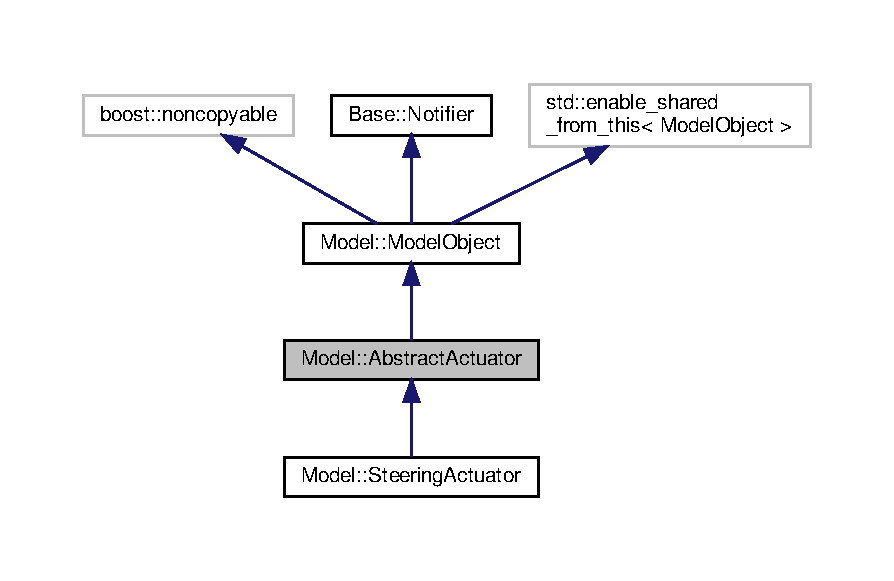
\includegraphics[width=350pt]{class_model_1_1_abstract_actuator__inherit__graph}
\end{center}
\end{figure}


Collaboration diagram for model\+:\+:Abstract\+Actuator\+:
\nopagebreak
\begin{figure}[H]
\begin{center}
\leavevmode
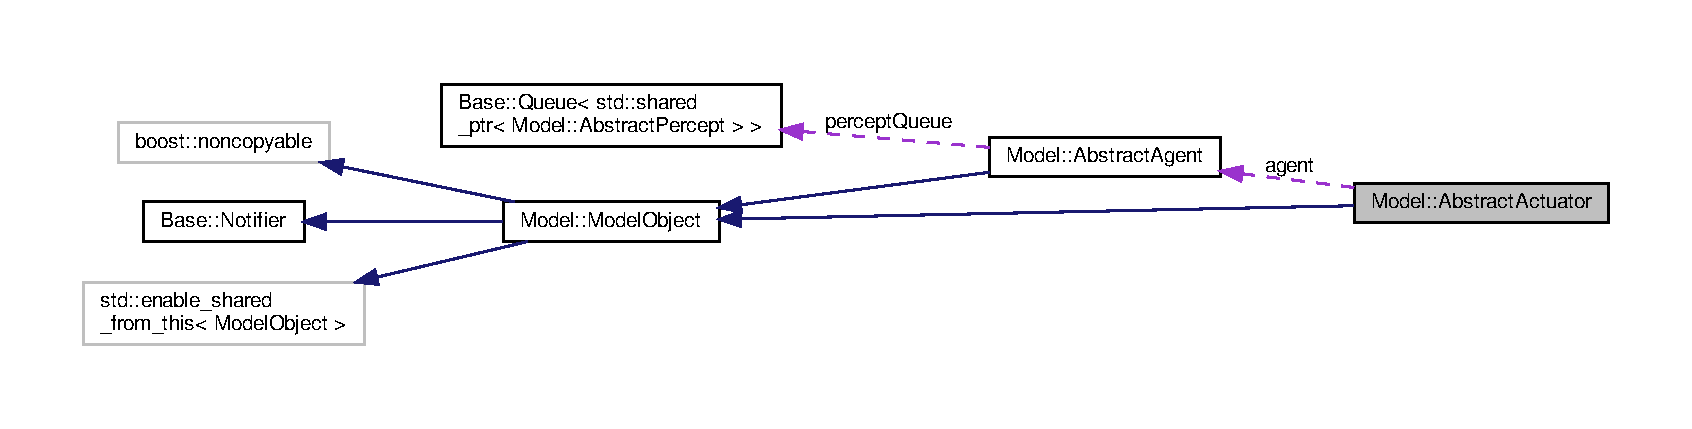
\includegraphics[width=350pt]{class_model_1_1_abstract_actuator__coll__graph}
\end{center}
\end{figure}
\subsection*{Public Member Functions}
\begin{DoxyCompactItemize}
\item 
{\bfseries Abstract\+Actuator} (\hyperlink{class_model_1_1_abstract_agent}{Abstract\+Agent} $\ast$an\+Agent)\hypertarget{class_model_1_1_abstract_actuator_a9137214d1e7cdb2939c90a858d451ac9}{}\label{class_model_1_1_abstract_actuator_a9137214d1e7cdb2939c90a858d451ac9}

\item 
virtual void {\bfseries handle\+Command} (\hyperlink{class_model_1_1_abstract_command}{Abstract\+Command} \&an\+Abstract\+Command)=0\hypertarget{class_model_1_1_abstract_actuator_adc357b727d6df7f1b0e0238c85fa99b2}{}\label{class_model_1_1_abstract_actuator_adc357b727d6df7f1b0e0238c85fa99b2}

\item 
virtual void {\bfseries attach\+Agent} (\hyperlink{class_model_1_1_abstract_agent}{Abstract\+Agent} $\ast$an\+Agent)\hypertarget{class_model_1_1_abstract_actuator_a36eb339606068a2dd22c5638628077ea}{}\label{class_model_1_1_abstract_actuator_a36eb339606068a2dd22c5638628077ea}

\item 
virtual void {\bfseries detach\+Agent} ()\hypertarget{class_model_1_1_abstract_actuator_a6499da8f728e56e4bfe6ae3b8601d2ec}{}\label{class_model_1_1_abstract_actuator_a6499da8f728e56e4bfe6ae3b8601d2ec}

\end{DoxyCompactItemize}
\begin{Indent}{\bf Debug functions}\par
\begin{DoxyCompactItemize}
\item 
virtual std\+::string \hyperlink{class_model_1_1_abstract_actuator_a6fe9d0ac0c7c6c56176fff61a773a4b9}{as\+String} () const 
\item 
virtual std\+::string \hyperlink{class_model_1_1_abstract_actuator_ab5199d4458a2913844459832d563f989}{as\+Debug\+String} () const 
\end{DoxyCompactItemize}
\end{Indent}
\subsection*{Protected Attributes}
\begin{DoxyCompactItemize}
\item 
\hyperlink{class_model_1_1_abstract_agent}{Abstract\+Agent} $\ast$ {\bfseries agent}\hypertarget{class_model_1_1_abstract_actuator_ad1067c897d696580dc7bc5713d1357d7}{}\label{class_model_1_1_abstract_actuator_ad1067c897d696580dc7bc5713d1357d7}

\end{DoxyCompactItemize}


\subsection{Member Function Documentation}
\index{model\+::\+Abstract\+Actuator@{model\+::\+Abstract\+Actuator}!as\+Debug\+String@{as\+Debug\+String}}
\index{as\+Debug\+String@{as\+Debug\+String}!model\+::\+Abstract\+Actuator@{model\+::\+Abstract\+Actuator}}
\subsubsection[{\texorpdfstring{as\+Debug\+String() const }{asDebugString() const }}]{\setlength{\rightskip}{0pt plus 5cm}std\+::string model\+::\+Abstract\+Actuator\+::as\+Debug\+String (
\begin{DoxyParamCaption}
{}
\end{DoxyParamCaption}
) const\hspace{0.3cm}{\ttfamily [virtual]}}\hypertarget{class_model_1_1_abstract_actuator_ab5199d4458a2913844459832d563f989}{}\label{class_model_1_1_abstract_actuator_ab5199d4458a2913844459832d563f989}
Returns a description of the object with all data of the object usable for debugging 

Reimplemented from \hyperlink{class_model_1_1_model_object_aced22b0b0ee637c598c463de6a1d8d03}{model\+::\+model\+Object}.

\index{model\+::\+Abstract\+Actuator@{model\+::\+Abstract\+Actuator}!as\+String@{as\+String}}
\index{as\+String@{as\+String}!model\+::\+Abstract\+Actuator@{model\+::\+Abstract\+Actuator}}
\subsubsection[{\texorpdfstring{as\+String() const }{asString() const }}]{\setlength{\rightskip}{0pt plus 5cm}std\+::string model\+::\+Abstract\+Actuator\+::as\+String (
\begin{DoxyParamCaption}
{}
\end{DoxyParamCaption}
) const\hspace{0.3cm}{\ttfamily [virtual]}}\hypertarget{class_model_1_1_abstract_actuator_a6fe9d0ac0c7c6c56176fff61a773a4b9}{}\label{class_model_1_1_abstract_actuator_a6fe9d0ac0c7c6c56176fff61a773a4b9}
Returns a 1-\/line description of the object 

Reimplemented from \hyperlink{class_model_1_1_model_object_a9db00b9150a932a1637e425f24c0bdf0}{model\+::\+model\+Object}.



The documentation for this class was generated from the following files\+:\begin{DoxyCompactItemize}
\item 
/home/hqnders/\+Documents/robotworld/src/Abstract\+Actuator.\+hpp\item 
/home/hqnders/\+Documents/robotworld/src/Abstract\+Actuator.\+cpp\end{DoxyCompactItemize}

\hypertarget{class_model_1_1_abstract_agent}{}\section{model\+:\+:Abstract\+Agent Class Reference}
\label{class_model_1_1_abstract_agent}\index{model\+::\+Abstract\+Agent@{model\+::\+Abstract\+Agent}}


Inheritance diagram for model\+:\+:Abstract\+Agent\+:
\nopagebreak
\begin{figure}[H]
\begin{center}
\leavevmode
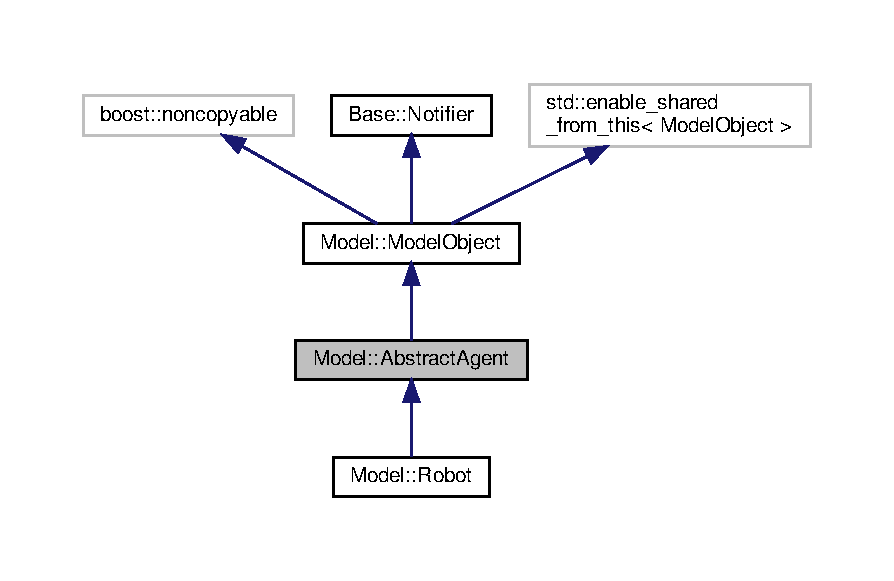
\includegraphics[width=350pt]{class_model_1_1_abstract_agent__inherit__graph}
\end{center}
\end{figure}


Collaboration diagram for model\+:\+:Abstract\+Agent\+:
\nopagebreak
\begin{figure}[H]
\begin{center}
\leavevmode
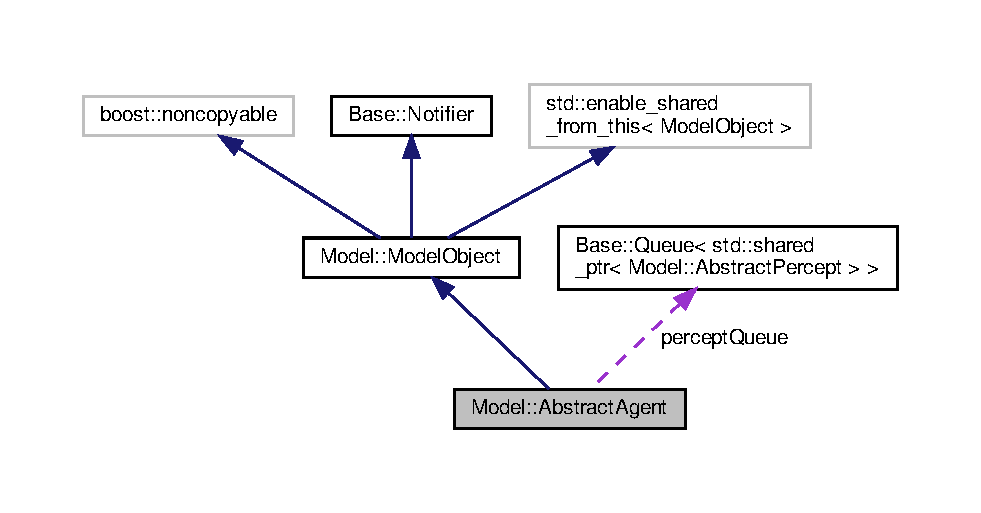
\includegraphics[width=350pt]{class_model_1_1_abstract_agent__coll__graph}
\end{center}
\end{figure}
\subsection*{Public Member Functions}
\begin{DoxyCompactItemize}
\item 
virtual void {\bfseries attach\+Sensor} (std\+::shared\+\_\+ptr$<$ \hyperlink{class_model_1_1_abstract_sensor}{Abstract\+Sensor} $>$ a\+Sensor, bool attach\+Sensor\+To\+Agent=false)\hypertarget{class_model_1_1_abstract_agent_a9e9a85420a923bb7d68acbda8208e2ad}{}\label{class_model_1_1_abstract_agent_a9e9a85420a923bb7d68acbda8208e2ad}

\item 
virtual void {\bfseries attach\+Actuator} (std\+::shared\+\_\+ptr$<$ \hyperlink{class_model_1_1_abstract_actuator}{Abstract\+Actuator} $>$ an\+Actuator, bool attach\+Actuator\+To\+Agent=false)\hypertarget{class_model_1_1_abstract_agent_a87cba14848a2ef4ec831ed2e44e85b63}{}\label{class_model_1_1_abstract_agent_a87cba14848a2ef4ec831ed2e44e85b63}

\item 
virtual void {\bfseries add\+Percept} (std\+::shared\+\_\+ptr$<$ \hyperlink{class_model_1_1_abstract_percept}{Abstract\+Percept} $>$ an\+Abstract\+Percept)\hypertarget{class_model_1_1_abstract_agent_ab8fb558bec05bc1a7ea5402bf996705f}{}\label{class_model_1_1_abstract_agent_ab8fb558bec05bc1a7ea5402bf996705f}

\item 
virtual void {\bfseries start\+Acting} ()=0\hypertarget{class_model_1_1_abstract_agent_a783133675cf1d592a95eadcbded59d2e}{}\label{class_model_1_1_abstract_agent_a783133675cf1d592a95eadcbded59d2e}

\item 
virtual void {\bfseries stop\+Acting} ()=0\hypertarget{class_model_1_1_abstract_agent_a369070540beac48686890b06d831fabe}{}\label{class_model_1_1_abstract_agent_a369070540beac48686890b06d831fabe}

\end{DoxyCompactItemize}
\begin{Indent}{\bf Debug functions}\par
\begin{DoxyCompactItemize}
\item 
virtual std\+::string \hyperlink{class_model_1_1_abstract_agent_a4cee6603af332eb80d524bf3af70489a}{as\+String} () const 
\item 
virtual std\+::string \hyperlink{class_model_1_1_abstract_agent_abcb33490b0f5761a2659bf705aff04b5}{as\+Debug\+String} () const 
\end{DoxyCompactItemize}
\end{Indent}
\subsection*{Protected Attributes}
\begin{DoxyCompactItemize}
\item 
std\+::vector$<$ std\+::shared\+\_\+ptr$<$ \hyperlink{class_model_1_1_abstract_sensor}{Abstract\+Sensor} $>$ $>$ {\bfseries sensors}\hypertarget{class_model_1_1_abstract_agent_a0235b5c010dedd813b12ae7e97cc4e2e}{}\label{class_model_1_1_abstract_agent_a0235b5c010dedd813b12ae7e97cc4e2e}

\item 
std\+::vector$<$ std\+::shared\+\_\+ptr$<$ \hyperlink{class_model_1_1_abstract_actuator}{Abstract\+Actuator} $>$ $>$ {\bfseries actuators}\hypertarget{class_model_1_1_abstract_agent_a23cd2a046e9e782f44a3dc0685fa84ca}{}\label{class_model_1_1_abstract_agent_a23cd2a046e9e782f44a3dc0685fa84ca}

\item 
\hyperlink{class_base_1_1_queue}{Base\+::\+Queue}$<$ std\+::shared\+\_\+ptr$<$ \hyperlink{class_model_1_1_abstract_percept}{Abstract\+Percept} $>$ $>$ {\bfseries percept\+Queue}\hypertarget{class_model_1_1_abstract_agent_ae49bfbbddb9c9a76478ec12f4760d127}{}\label{class_model_1_1_abstract_agent_ae49bfbbddb9c9a76478ec12f4760d127}

\end{DoxyCompactItemize}


\subsection{Member Function Documentation}
\index{model\+::\+Abstract\+Agent@{model\+::\+Abstract\+Agent}!as\+Debug\+String@{as\+Debug\+String}}
\index{as\+Debug\+String@{as\+Debug\+String}!model\+::\+Abstract\+Agent@{model\+::\+Abstract\+Agent}}
\subsubsection[{\texorpdfstring{as\+Debug\+String() const }{asDebugString() const }}]{\setlength{\rightskip}{0pt plus 5cm}std\+::string model\+::\+Abstract\+Agent\+::as\+Debug\+String (
\begin{DoxyParamCaption}
{}
\end{DoxyParamCaption}
) const\hspace{0.3cm}{\ttfamily [virtual]}}\hypertarget{class_model_1_1_abstract_agent_abcb33490b0f5761a2659bf705aff04b5}{}\label{class_model_1_1_abstract_agent_abcb33490b0f5761a2659bf705aff04b5}
Returns a description of the object with all data of the object usable for debugging 

Reimplemented from \hyperlink{class_model_1_1_model_object_aced22b0b0ee637c598c463de6a1d8d03}{model\+::\+model\+Object}.



Reimplemented in \hyperlink{class_model_1_1_robot_aaf05b81b0aff3dac7b39effa462da04e}{model\+::\+Robot}.

\index{model\+::\+Abstract\+Agent@{model\+::\+Abstract\+Agent}!as\+String@{as\+String}}
\index{as\+String@{as\+String}!model\+::\+Abstract\+Agent@{model\+::\+Abstract\+Agent}}
\subsubsection[{\texorpdfstring{as\+String() const }{asString() const }}]{\setlength{\rightskip}{0pt plus 5cm}std\+::string model\+::\+Abstract\+Agent\+::as\+String (
\begin{DoxyParamCaption}
{}
\end{DoxyParamCaption}
) const\hspace{0.3cm}{\ttfamily [virtual]}}\hypertarget{class_model_1_1_abstract_agent_a4cee6603af332eb80d524bf3af70489a}{}\label{class_model_1_1_abstract_agent_a4cee6603af332eb80d524bf3af70489a}
Returns a 1-\/line description of the object 

Reimplemented from \hyperlink{class_model_1_1_model_object_a9db00b9150a932a1637e425f24c0bdf0}{model\+::\+model\+Object}.



Reimplemented in \hyperlink{class_model_1_1_robot_a888add69a87a3e0f82a3f9c95140716f}{model\+::\+Robot}.



The documentation for this class was generated from the following files\+:\begin{DoxyCompactItemize}
\item 
/home/hqnders/\+Documents/robotworld/src/Abstract\+Agent.\+hpp\item 
/home/hqnders/\+Documents/robotworld/src/Abstract\+Agent.\+cpp\end{DoxyCompactItemize}

\hypertarget{class_model_1_1_abstract_command}{}\section{model\+:\+:Abstract\+Command Class Reference}
\label{class_model_1_1_abstract_command}\index{model\+::\+Abstract\+Command@{model\+::\+Abstract\+Command}}


The documentation for this class was generated from the following file\+:\begin{DoxyCompactItemize}
\item 
/home/hqnders/\+Documents/robotworld/src/Abstract\+Actuator.\+hpp\end{DoxyCompactItemize}

\hypertarget{class_model_1_1_abstract_percept}{}\section{model\+:\+:Abstract\+Percept Class Reference}
\label{class_model_1_1_abstract_percept}\index{model\+::\+Abstract\+Percept@{model\+::\+Abstract\+Percept}}


Inheritance diagram for model\+:\+:Abstract\+Percept\+:
\nopagebreak
\begin{figure}[H]
\begin{center}
\leavevmode
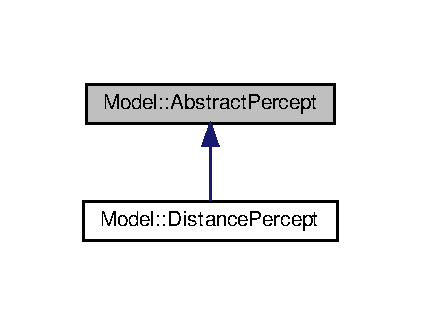
\includegraphics[width=202pt]{class_model_1_1_abstract_percept__inherit__graph}
\end{center}
\end{figure}


The documentation for this class was generated from the following file\+:\begin{DoxyCompactItemize}
\item 
/home/hqnders/\+Documents/robotworld/src/Abstract\+Sensor.\+hpp\end{DoxyCompactItemize}

\hypertarget{class_model_1_1_abstract_sensor}{}\section{model\+:\+:Abstract\+Sensor Class Reference}
\label{class_model_1_1_abstract_sensor}\index{model\+::\+Abstract\+Sensor@{model\+::\+Abstract\+Sensor}}


Inheritance diagram for model\+:\+:Abstract\+Sensor\+:
\nopagebreak
\begin{figure}[H]
\begin{center}
\leavevmode
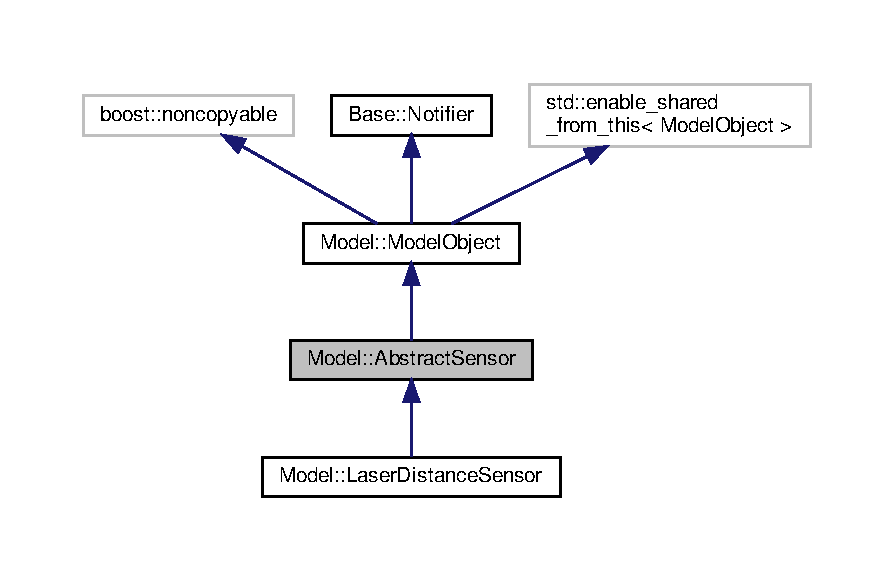
\includegraphics[width=350pt]{class_model_1_1_abstract_sensor__inherit__graph}
\end{center}
\end{figure}


Collaboration diagram for model\+:\+:Abstract\+Sensor\+:
\nopagebreak
\begin{figure}[H]
\begin{center}
\leavevmode
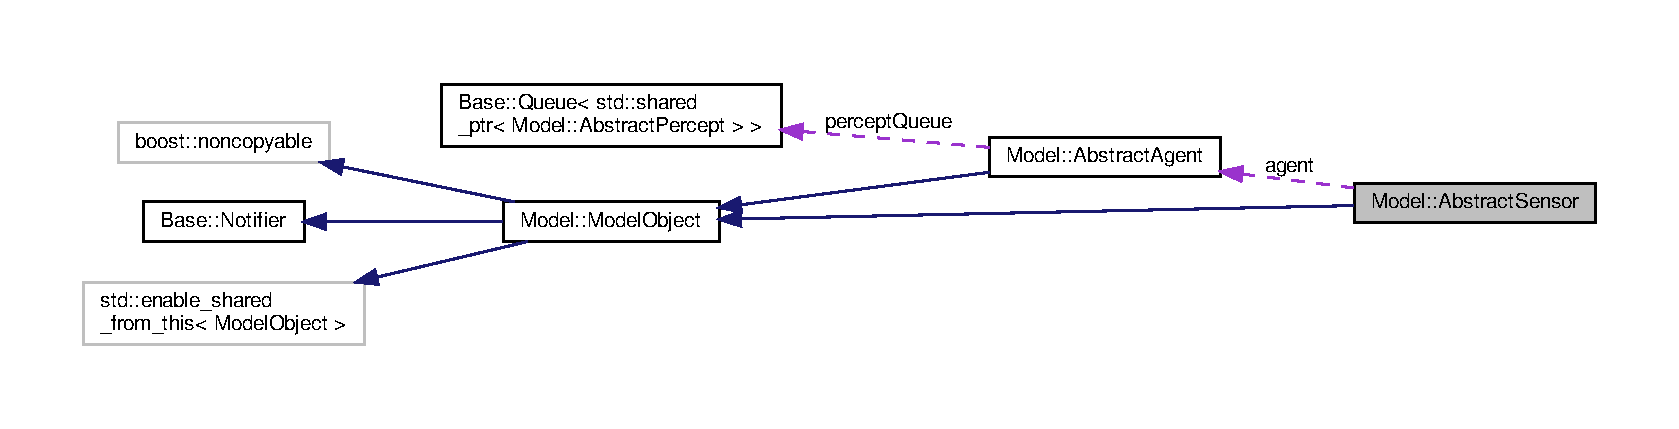
\includegraphics[width=350pt]{class_model_1_1_abstract_sensor__coll__graph}
\end{center}
\end{figure}
\subsection*{Public Member Functions}
\begin{DoxyCompactItemize}
\item 
{\bfseries Abstract\+Sensor} (\hyperlink{class_model_1_1_abstract_agent}{Abstract\+Agent} $\ast$an\+Agent)\hypertarget{class_model_1_1_abstract_sensor_a787a53fde6320acca0a3500221f11bf4}{}\label{class_model_1_1_abstract_sensor_a787a53fde6320acca0a3500221f11bf4}

\item 
virtual void \hyperlink{class_model_1_1_abstract_sensor_a958bad26decf903bb28fd45bc835c7bb}{set\+On} (unsigned long a\+Sleep\+Time=100)
\item 
virtual void {\bfseries set\+Off} ()\hypertarget{class_model_1_1_abstract_sensor_a31f0eb53ed8252c45e4ac64ea328d7b9}{}\label{class_model_1_1_abstract_sensor_a31f0eb53ed8252c45e4ac64ea328d7b9}

\item 
virtual std\+::shared\+\_\+ptr$<$ \hyperlink{class_model_1_1_abstract_stimulus}{Abstract\+Stimulus} $>$ {\bfseries get\+Stimulus} () const =0\hypertarget{class_model_1_1_abstract_sensor_a63ae4aa9e8ac1592f48dbdb1b734ddde}{}\label{class_model_1_1_abstract_sensor_a63ae4aa9e8ac1592f48dbdb1b734ddde}

\item 
virtual std\+::shared\+\_\+ptr$<$ \hyperlink{class_model_1_1_abstract_percept}{Abstract\+Percept} $>$ {\bfseries get\+Percept\+For} (std\+::shared\+\_\+ptr$<$ \hyperlink{class_model_1_1_abstract_stimulus}{Abstract\+Stimulus} $>$ an\+Abstract\+Percepts) const =0\hypertarget{class_model_1_1_abstract_sensor_ac9254468d847d18b0895b9fa29fb7871}{}\label{class_model_1_1_abstract_sensor_ac9254468d847d18b0895b9fa29fb7871}

\item 
virtual void {\bfseries send\+Percept} (std\+::shared\+\_\+ptr$<$ \hyperlink{class_model_1_1_abstract_percept}{Abstract\+Percept} $>$ an\+Abstract\+Percept)\hypertarget{class_model_1_1_abstract_sensor_a2b0fb54fe519b4c58187b939ec612eb0}{}\label{class_model_1_1_abstract_sensor_a2b0fb54fe519b4c58187b939ec612eb0}

\item 
virtual void {\bfseries run} (unsigned long a\+Sleep\+Time)\hypertarget{class_model_1_1_abstract_sensor_ab85ffa9f6dbdf249681ed95a052bf017}{}\label{class_model_1_1_abstract_sensor_ab85ffa9f6dbdf249681ed95a052bf017}

\item 
virtual void {\bfseries attach\+Agent} (\hyperlink{class_model_1_1_abstract_agent}{Abstract\+Agent} $\ast$an\+Agent)\hypertarget{class_model_1_1_abstract_sensor_ad78d0c553f653f564fbbe222a1a8bd81}{}\label{class_model_1_1_abstract_sensor_ad78d0c553f653f564fbbe222a1a8bd81}

\item 
virtual void {\bfseries detach\+Agent} ()\hypertarget{class_model_1_1_abstract_sensor_ab6bc01195b77d486d7ea628f731416db}{}\label{class_model_1_1_abstract_sensor_ab6bc01195b77d486d7ea628f731416db}

\end{DoxyCompactItemize}
\begin{Indent}{\bf Debug functions}\par
\begin{DoxyCompactItemize}
\item 
virtual std\+::string \hyperlink{class_model_1_1_abstract_sensor_a85c18d6d51b8b6a3b97f682ad242be9d}{as\+String} () const 
\item 
virtual std\+::string \hyperlink{class_model_1_1_abstract_sensor_aa67bce32b6a602772773f0f23d0634f0}{as\+Debug\+String} () const 
\end{DoxyCompactItemize}
\end{Indent}
\subsection*{Protected Attributes}
\begin{DoxyCompactItemize}
\item 
\hyperlink{class_model_1_1_abstract_agent}{Abstract\+Agent} $\ast$ {\bfseries agent}\hypertarget{class_model_1_1_abstract_sensor_acc26be4569ca92c524e3759f8bda8e36}{}\label{class_model_1_1_abstract_sensor_acc26be4569ca92c524e3759f8bda8e36}

\item 
bool {\bfseries running}\hypertarget{class_model_1_1_abstract_sensor_ad4cbae39fd0117e9917c33a6a7f09fa5}{}\label{class_model_1_1_abstract_sensor_ad4cbae39fd0117e9917c33a6a7f09fa5}

\item 
\hyperlink{namespacestd_af8ef78a9cf464d7f7faf334b0648cd20}{std\+::thread} {\bfseries sensor\+Thread}\hypertarget{class_model_1_1_abstract_sensor_a7de4321e9fa04d352cd42b7f33e2ce9c}{}\label{class_model_1_1_abstract_sensor_a7de4321e9fa04d352cd42b7f33e2ce9c}

\item 
std\+::recursive\+\_\+mutex {\bfseries sensor\+Mutex}\hypertarget{class_model_1_1_abstract_sensor_ab8de89a6213d2a76d930e02a3cac3947}{}\label{class_model_1_1_abstract_sensor_ab8de89a6213d2a76d930e02a3cac3947}

\end{DoxyCompactItemize}


\subsection{Member Function Documentation}
\index{model\+::\+Abstract\+Sensor@{model\+::\+Abstract\+Sensor}!as\+Debug\+String@{as\+Debug\+String}}
\index{as\+Debug\+String@{as\+Debug\+String}!model\+::\+Abstract\+Sensor@{model\+::\+Abstract\+Sensor}}
\subsubsection[{\texorpdfstring{as\+Debug\+String() const }{asDebugString() const }}]{\setlength{\rightskip}{0pt plus 5cm}std\+::string model\+::\+Abstract\+Sensor\+::as\+Debug\+String (
\begin{DoxyParamCaption}
{}
\end{DoxyParamCaption}
) const\hspace{0.3cm}{\ttfamily [virtual]}}\hypertarget{class_model_1_1_abstract_sensor_aa67bce32b6a602772773f0f23d0634f0}{}\label{class_model_1_1_abstract_sensor_aa67bce32b6a602772773f0f23d0634f0}
Returns a description of the object with all data of the object usable for debugging 

Reimplemented from \hyperlink{class_model_1_1_model_object_aced22b0b0ee637c598c463de6a1d8d03}{model\+::\+model\+Object}.



Reimplemented in \hyperlink{class_model_1_1_laser_distance_sensor_ab32d7cbfd19a9a5ec12a0c06ebb02b4f}{model\+::\+Laser\+Distance\+Sensor}.

\index{model\+::\+Abstract\+Sensor@{model\+::\+Abstract\+Sensor}!as\+String@{as\+String}}
\index{as\+String@{as\+String}!model\+::\+Abstract\+Sensor@{model\+::\+Abstract\+Sensor}}
\subsubsection[{\texorpdfstring{as\+String() const }{asString() const }}]{\setlength{\rightskip}{0pt plus 5cm}std\+::string model\+::\+Abstract\+Sensor\+::as\+String (
\begin{DoxyParamCaption}
{}
\end{DoxyParamCaption}
) const\hspace{0.3cm}{\ttfamily [virtual]}}\hypertarget{class_model_1_1_abstract_sensor_a85c18d6d51b8b6a3b97f682ad242be9d}{}\label{class_model_1_1_abstract_sensor_a85c18d6d51b8b6a3b97f682ad242be9d}
Returns a 1-\/line description of the object 

Reimplemented from \hyperlink{class_model_1_1_model_object_a9db00b9150a932a1637e425f24c0bdf0}{model\+::\+model\+Object}.



Reimplemented in \hyperlink{class_model_1_1_laser_distance_sensor_a9403593acd21d557e5af1d79901fde34}{model\+::\+Laser\+Distance\+Sensor}.

\index{model\+::\+Abstract\+Sensor@{model\+::\+Abstract\+Sensor}!set\+On@{set\+On}}
\index{set\+On@{set\+On}!model\+::\+Abstract\+Sensor@{model\+::\+Abstract\+Sensor}}
\subsubsection[{\texorpdfstring{set\+On(unsigned long a\+Sleep\+Time=100)}{setOn(unsigned long aSleepTime=100)}}]{\setlength{\rightskip}{0pt plus 5cm}void model\+::\+Abstract\+Sensor\+::set\+On (
\begin{DoxyParamCaption}
\item[{unsigned long}]{a\+Sleep\+Time = {\ttfamily 100}}
\end{DoxyParamCaption}
)\hspace{0.3cm}{\ttfamily [virtual]}}\hypertarget{class_model_1_1_abstract_sensor_a958bad26decf903bb28fd45bc835c7bb}{}\label{class_model_1_1_abstract_sensor_a958bad26decf903bb28fd45bc835c7bb}
A sensor reads 10 stimuli/second (it sleeps for 100 ms) by default 

The documentation for this class was generated from the following files\+:\begin{DoxyCompactItemize}
\item 
/home/hqnders/\+Documents/robotworld/src/Abstract\+Sensor.\+hpp\item 
/home/hqnders/\+Documents/robotworld/src/Abstract\+Sensor.\+cpp\end{DoxyCompactItemize}

\hypertarget{class_model_1_1_abstract_stimulus}{}\section{model\+:\+:Abstract\+Stimulus Class Reference}
\label{class_model_1_1_abstract_stimulus}\index{model\+::\+Abstract\+Stimulus@{model\+::\+Abstract\+Stimulus}}


Inheritance diagram for model\+:\+:Abstract\+Stimulus\+:
\nopagebreak
\begin{figure}[H]
\begin{center}
\leavevmode
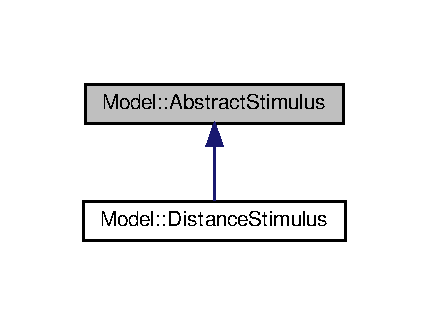
\includegraphics[width=206pt]{class_model_1_1_abstract_stimulus__inherit__graph}
\end{center}
\end{figure}


The documentation for this class was generated from the following file\+:\begin{DoxyCompactItemize}
\item 
/home/hqnders/\+Documents/robotworld/src/Abstract\+Sensor.\+hpp\end{DoxyCompactItemize}

\hypertarget{class_path_algorithm_1_1_a_star}{}\section{Path\+Algorithm\+:\+:A\+Star Class Reference}
\label{class_path_algorithm_1_1_a_star}\index{Path\+Algorithm\+::\+A\+Star@{Path\+Algorithm\+::\+A\+Star}}


Inheritance diagram for Path\+Algorithm\+:\+:A\+Star\+:
\nopagebreak
\begin{figure}[H]
\begin{center}
\leavevmode
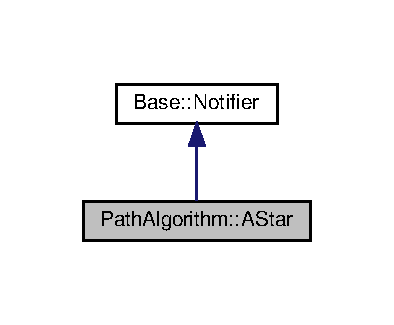
\includegraphics[width=189pt]{class_path_algorithm_1_1_a_star__inherit__graph}
\end{center}
\end{figure}


Collaboration diagram for Path\+Algorithm\+:\+:A\+Star\+:
\nopagebreak
\begin{figure}[H]
\begin{center}
\leavevmode
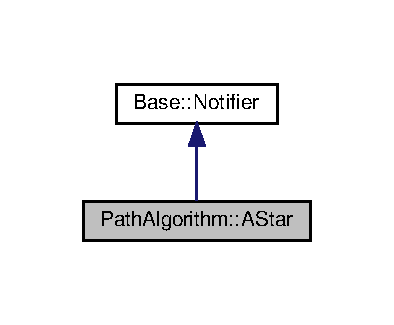
\includegraphics[width=189pt]{class_path_algorithm_1_1_a_star__coll__graph}
\end{center}
\end{figure}
\subsection*{Public Member Functions}
\begin{DoxyCompactItemize}
\item 
Path {\bfseries search} (const Point \&a\+Start\+Point, const Point \&a\+Goal\+Point, const Size \&a\+Robot\+Size)\hypertarget{class_path_algorithm_1_1_a_star_a9112cf1a7a2e991046d88a1f5cba8925}{}\label{class_path_algorithm_1_1_a_star_a9112cf1a7a2e991046d88a1f5cba8925}

\item 
Path {\bfseries search} (\hyperlink{struct_path_algorithm_1_1_vertex}{Vertex} a\+Start, const \hyperlink{struct_path_algorithm_1_1_vertex}{Vertex} \&a\+Goal, const Size \&a\+Robot\+Size)\hypertarget{class_path_algorithm_1_1_a_star_a08d4471b622ff7cef2d6a65af869ceb3}{}\label{class_path_algorithm_1_1_a_star_a08d4471b622ff7cef2d6a65af869ceb3}

\item 
void {\bfseries add\+To\+Open\+Set} (const \hyperlink{struct_path_algorithm_1_1_vertex}{Vertex} \&a\+Vertex)\hypertarget{class_path_algorithm_1_1_a_star_a63f88f24acf7bf34cd060051134c9190}{}\label{class_path_algorithm_1_1_a_star_a63f88f24acf7bf34cd060051134c9190}

\item 
void {\bfseries remove\+From\+Open\+Set} (const \hyperlink{struct_path_algorithm_1_1_vertex}{Vertex} \&a\+Vertex)\hypertarget{class_path_algorithm_1_1_a_star_afcc23a676145d6e280d1c3430af5380a}{}\label{class_path_algorithm_1_1_a_star_afcc23a676145d6e280d1c3430af5380a}

\item 
void {\bfseries remove\+From\+Open\+Set} (Open\+Set\+::iterator \&i)\hypertarget{class_path_algorithm_1_1_a_star_aba29c2585fbf49880cf5e8b9bf6d3eb5}{}\label{class_path_algorithm_1_1_a_star_aba29c2585fbf49880cf5e8b9bf6d3eb5}

\item 
Open\+Set\+::iterator {\bfseries find\+In\+Open\+Set} (const \hyperlink{struct_path_algorithm_1_1_vertex}{Vertex} \&a\+Vertex)\hypertarget{class_path_algorithm_1_1_a_star_ae78bfebdee31135fdfb2f302347f962f}{}\label{class_path_algorithm_1_1_a_star_ae78bfebdee31135fdfb2f302347f962f}

\item 
bool {\bfseries find\+Remove\+In\+Open\+Set} (const \hyperlink{struct_path_algorithm_1_1_vertex}{Vertex} \&a\+Vertex)\hypertarget{class_path_algorithm_1_1_a_star_a657aaaf577ca25e68e6a5af57214e7d4}{}\label{class_path_algorithm_1_1_a_star_a657aaaf577ca25e68e6a5af57214e7d4}

\item 
void {\bfseries remove\+First\+From\+Open\+Set} ()\hypertarget{class_path_algorithm_1_1_a_star_a5bb18edbbd54833aac9eddfe63ba652d}{}\label{class_path_algorithm_1_1_a_star_a5bb18edbbd54833aac9eddfe63ba652d}

\item 
void {\bfseries add\+To\+Closed\+Set} (const \hyperlink{struct_path_algorithm_1_1_vertex}{Vertex} \&a\+Vertex)\hypertarget{class_path_algorithm_1_1_a_star_a53139e4b3cd3971a2bf85a430e83378f}{}\label{class_path_algorithm_1_1_a_star_a53139e4b3cd3971a2bf85a430e83378f}

\item 
void {\bfseries remove\+From\+Closed\+Set} (const \hyperlink{struct_path_algorithm_1_1_vertex}{Vertex} \&a\+Vertex)\hypertarget{class_path_algorithm_1_1_a_star_a1b6971a9c5878e859cbdb3270dda93b4}{}\label{class_path_algorithm_1_1_a_star_a1b6971a9c5878e859cbdb3270dda93b4}

\item 
void {\bfseries remove\+From\+Closed\+Set} (Closed\+Set\+::iterator \&i)\hypertarget{class_path_algorithm_1_1_a_star_a799953993c1255f0ce559f7233d3c926}{}\label{class_path_algorithm_1_1_a_star_a799953993c1255f0ce559f7233d3c926}

\item 
Closed\+Set\+::iterator {\bfseries find\+In\+Closed\+Set} (const \hyperlink{struct_path_algorithm_1_1_vertex}{Vertex} \&a\+Vertex)\hypertarget{class_path_algorithm_1_1_a_star_a73d9639e838fd55bb392d01238fc967a}{}\label{class_path_algorithm_1_1_a_star_a73d9639e838fd55bb392d01238fc967a}

\item 
bool {\bfseries find\+Remove\+Closed\+Set} (const \hyperlink{struct_path_algorithm_1_1_vertex}{Vertex} \&a\+Vertex)\hypertarget{class_path_algorithm_1_1_a_star_a843db81c9950c0184ee31627313f5793}{}\label{class_path_algorithm_1_1_a_star_a843db81c9950c0184ee31627313f5793}

\item 
Closed\+Set {\bfseries get\+Closed\+Set} () const \hypertarget{class_path_algorithm_1_1_a_star_a94fcc29f04e6398edbd58effbf59b49a}{}\label{class_path_algorithm_1_1_a_star_a94fcc29f04e6398edbd58effbf59b49a}

\item 
Open\+Set {\bfseries get\+Open\+Set} () const \hypertarget{class_path_algorithm_1_1_a_star_ae419f2d019378d9b4435d862b70da72f}{}\label{class_path_algorithm_1_1_a_star_ae419f2d019378d9b4435d862b70da72f}

\item 
Vertex\+Map {\bfseries get\+Predecessor\+Map} () const \hypertarget{class_path_algorithm_1_1_a_star_ac4ce233712c0f7aac44d029e61888581}{}\label{class_path_algorithm_1_1_a_star_ac4ce233712c0f7aac44d029e61888581}

\end{DoxyCompactItemize}
\subsection*{Protected Member Functions}
\begin{DoxyCompactItemize}
\item 
Closed\+Set \& {\bfseries get\+CS} ()\hypertarget{class_path_algorithm_1_1_a_star_a4cb2a6c928a01fcac02533500bd8ace5}{}\label{class_path_algorithm_1_1_a_star_a4cb2a6c928a01fcac02533500bd8ace5}

\item 
const Closed\+Set \& {\bfseries get\+CS} () const \hypertarget{class_path_algorithm_1_1_a_star_a420e1ac8824a265dc2272c7e50899322}{}\label{class_path_algorithm_1_1_a_star_a420e1ac8824a265dc2272c7e50899322}

\item 
Open\+Set \& {\bfseries get\+OS} ()\hypertarget{class_path_algorithm_1_1_a_star_a48e23107ffca02392bdf2439775baecf}{}\label{class_path_algorithm_1_1_a_star_a48e23107ffca02392bdf2439775baecf}

\item 
const Open\+Set \& {\bfseries get\+OS} () const \hypertarget{class_path_algorithm_1_1_a_star_af5ea4271f9318edaa68d8030e35d0cf1}{}\label{class_path_algorithm_1_1_a_star_af5ea4271f9318edaa68d8030e35d0cf1}

\item 
Vertex\+Map \& {\bfseries get\+PM} ()\hypertarget{class_path_algorithm_1_1_a_star_a4bb6718fd07f503ff836c5cdccd74236}{}\label{class_path_algorithm_1_1_a_star_a4bb6718fd07f503ff836c5cdccd74236}

\item 
const Vertex\+Map \& {\bfseries get\+PM} () const \hypertarget{class_path_algorithm_1_1_a_star_a021ff514f018ce9ec7db705578a210d4}{}\label{class_path_algorithm_1_1_a_star_a021ff514f018ce9ec7db705578a210d4}

\end{DoxyCompactItemize}


The documentation for this class was generated from the following files\+:\begin{DoxyCompactItemize}
\item 
/home/hqnders/\+Documents/robotworld/src/A\+Star.\+hpp\item 
/home/hqnders/\+Documents/robotworld/src/A\+Star.\+cpp\end{DoxyCompactItemize}

\hypertarget{class_model_1_1_bounded_vector}{}\section{model\+:\+:Bounded\+Vector Class Reference}
\label{class_model_1_1_bounded_vector}\index{model\+::\+Bounded\+Vector@{model\+::\+Bounded\+Vector}}
\subsection*{Public Member Functions}
\begin{DoxyCompactItemize}
\item 
{\bfseries Bounded\+Vector} (float anX, float anY)\hypertarget{class_model_1_1_bounded_vector_a55d60da08dc45930fe4b7db6aca8a55d}{}\label{class_model_1_1_bounded_vector_a55d60da08dc45930fe4b7db6aca8a55d}

\item 
{\bfseries Bounded\+Vector} (const Point \&a\+Point1, const Point \&a\+Point2)\hypertarget{class_model_1_1_bounded_vector_ab769d7fcd9ca402df947e5515c929515}{}\label{class_model_1_1_bounded_vector_ab769d7fcd9ca402df947e5515c929515}

\item 
{\bfseries Bounded\+Vector} (const \hyperlink{class_model_1_1_bounded_vector}{Bounded\+Vector} \&a\+Polar\+Coord)\hypertarget{class_model_1_1_bounded_vector_ab39ae90320b2e9e3f12ef25322620b18}{}\label{class_model_1_1_bounded_vector_ab39ae90320b2e9e3f12ef25322620b18}

\item 
float {\bfseries get\+Magnitude} ()\hypertarget{class_model_1_1_bounded_vector_a9cd9a0c3001c9a717b9fe7c38c4a791a}{}\label{class_model_1_1_bounded_vector_a9cd9a0c3001c9a717b9fe7c38c4a791a}

\item 
void {\bfseries normalise} ()\hypertarget{class_model_1_1_bounded_vector_a063e74d97117138fc2ed5fe7e007f133}{}\label{class_model_1_1_bounded_vector_a063e74d97117138fc2ed5fe7e007f133}

\item 
\hyperlink{class_model_1_1_bounded_vector}{Bounded\+Vector} {\bfseries get\+Normalised} ()\hypertarget{class_model_1_1_bounded_vector_a6a4148a2cf2298951d0b2469c33d799f}{}\label{class_model_1_1_bounded_vector_a6a4148a2cf2298951d0b2469c33d799f}

\item 
void {\bfseries reverse} ()\hypertarget{class_model_1_1_bounded_vector_a29b4dd3c012309ccdb622fab46da50cb}{}\label{class_model_1_1_bounded_vector_a29b4dd3c012309ccdb622fab46da50cb}

\item 
\hyperlink{class_model_1_1_bounded_vector}{Bounded\+Vector} \& {\bfseries operator+=} (const \hyperlink{class_model_1_1_bounded_vector}{Bounded\+Vector} \&a\+Vector)\hypertarget{class_model_1_1_bounded_vector_a6f707a9499dc1a1a4051fa2b40f8d40d}{}\label{class_model_1_1_bounded_vector_a6f707a9499dc1a1a4051fa2b40f8d40d}

\item 
\hyperlink{class_model_1_1_bounded_vector}{Bounded\+Vector} \& {\bfseries operator-\/=} (const \hyperlink{class_model_1_1_bounded_vector}{Bounded\+Vector} \&a\+Vector)\hypertarget{class_model_1_1_bounded_vector_ae1cb231bfe977d563eebfd47526cb1c0}{}\label{class_model_1_1_bounded_vector_ae1cb231bfe977d563eebfd47526cb1c0}

\item 
\hyperlink{class_model_1_1_bounded_vector}{Bounded\+Vector} \& {\bfseries operator$\ast$=} (float a\+Scalar)\hypertarget{class_model_1_1_bounded_vector_aeed3b7e66556126aee3478daa6f9199b}{}\label{class_model_1_1_bounded_vector_aeed3b7e66556126aee3478daa6f9199b}

\item 
\hyperlink{class_model_1_1_bounded_vector}{Bounded\+Vector} \& {\bfseries operator/=} (float a\+Scalar)\hypertarget{class_model_1_1_bounded_vector_ac949b337eed72116f01507c7bba5820a}{}\label{class_model_1_1_bounded_vector_ac949b337eed72116f01507c7bba5820a}

\item 
\hyperlink{class_model_1_1_bounded_vector}{Bounded\+Vector} {\bfseries operator-\/} ()\hypertarget{class_model_1_1_bounded_vector_a05b571d646e8c226c3bef443cbdb00f7}{}\label{class_model_1_1_bounded_vector_a05b571d646e8c226c3bef443cbdb00f7}

\end{DoxyCompactItemize}
\begin{Indent}{\bf Debug functions}\par
\begin{DoxyCompactItemize}
\item 
virtual std\+::string \hyperlink{class_model_1_1_bounded_vector_a5a0115cf9e87c118474d507efcbaddfb}{as\+String} () const 
\item 
virtual std\+::string \hyperlink{class_model_1_1_bounded_vector_aa04899e137a269e9ab116535c4fadc07}{as\+Debug\+String} () const 
\end{DoxyCompactItemize}
\end{Indent}
\subsection*{Public Attributes}
\begin{DoxyCompactItemize}
\item 
float {\bfseries x}\hypertarget{class_model_1_1_bounded_vector_a0d837ee4acabf638003a62c9d50a9935}{}\label{class_model_1_1_bounded_vector_a0d837ee4acabf638003a62c9d50a9935}

\item 
float {\bfseries y}\hypertarget{class_model_1_1_bounded_vector_a627a1a0ab97bd13e2d1b6ec179ad58ca}{}\label{class_model_1_1_bounded_vector_a627a1a0ab97bd13e2d1b6ec179ad58ca}

\end{DoxyCompactItemize}


\subsection{Member Function Documentation}
\index{model\+::\+Bounded\+Vector@{model\+::\+Bounded\+Vector}!as\+Debug\+String@{as\+Debug\+String}}
\index{as\+Debug\+String@{as\+Debug\+String}!model\+::\+Bounded\+Vector@{model\+::\+Bounded\+Vector}}
\subsubsection[{\texorpdfstring{as\+Debug\+String() const }{asDebugString() const }}]{\setlength{\rightskip}{0pt plus 5cm}std\+::string model\+::\+Bounded\+Vector\+::as\+Debug\+String (
\begin{DoxyParamCaption}
{}
\end{DoxyParamCaption}
) const\hspace{0.3cm}{\ttfamily [virtual]}}\hypertarget{class_model_1_1_bounded_vector_aa04899e137a269e9ab116535c4fadc07}{}\label{class_model_1_1_bounded_vector_aa04899e137a269e9ab116535c4fadc07}
Returns a description of the object with all data of the object usable for debugging \index{model\+::\+Bounded\+Vector@{model\+::\+Bounded\+Vector}!as\+String@{as\+String}}
\index{as\+String@{as\+String}!model\+::\+Bounded\+Vector@{model\+::\+Bounded\+Vector}}
\subsubsection[{\texorpdfstring{as\+String() const }{asString() const }}]{\setlength{\rightskip}{0pt plus 5cm}std\+::string model\+::\+Bounded\+Vector\+::as\+String (
\begin{DoxyParamCaption}
{}
\end{DoxyParamCaption}
) const\hspace{0.3cm}{\ttfamily [virtual]}}\hypertarget{class_model_1_1_bounded_vector_a5a0115cf9e87c118474d507efcbaddfb}{}\label{class_model_1_1_bounded_vector_a5a0115cf9e87c118474d507efcbaddfb}
Returns a 1-\/line description of the object 

The documentation for this class was generated from the following files\+:\begin{DoxyCompactItemize}
\item 
/home/hqnders/\+Documents/robotworld/src/Bounded\+Vector.\+hpp\item 
/home/hqnders/\+Documents/robotworld/src/Bounded\+Vector.\+cpp\end{DoxyCompactItemize}

\hypertarget{class_messaging_1_1_client}{}\section{Messaging\+:\+:Client Class Reference}
\label{class_messaging_1_1_client}\index{Messaging\+::\+Client@{Messaging\+::\+Client}}
\subsection*{Public Member Functions}
\begin{DoxyCompactItemize}
\item 
{\bfseries Client} (const std\+::string \&a\+Host, const std\+::string \&a\+Port, Response\+Handler\+Ptr a\+Response\+Handler)\hypertarget{class_messaging_1_1_client_a3d9868c2817f181e38f1e50e57faa25f}{}\label{class_messaging_1_1_client_a3d9868c2817f181e38f1e50e57faa25f}

\item 
void {\bfseries dispatch\+Message} (\hyperlink{struct_messaging_1_1_message}{Message} \&a\+Message)\hypertarget{class_messaging_1_1_client_ad591a306de7942562e5f682d4ec3b454}{}\label{class_messaging_1_1_client_ad591a306de7942562e5f682d4ec3b454}

\item 
void {\bfseries handle\+Connect} (\hyperlink{class_messaging_1_1_client_session}{Client\+Session} $\ast$a\+Session, const boost\+::system\+::error\+\_\+code \&error)\hypertarget{class_messaging_1_1_client_a7804792b483e50df149e9e77191d5d16}{}\label{class_messaging_1_1_client_a7804792b483e50df149e9e77191d5d16}

\end{DoxyCompactItemize}


The documentation for this class was generated from the following file\+:\begin{DoxyCompactItemize}
\item 
/home/hqnders/\+Documents/robotworld/src/Client.\+hpp\end{DoxyCompactItemize}

\hypertarget{class_messaging_1_1_client_session}{}\section{Messaging\+:\+:Client\+Session Class Reference}
\label{class_messaging_1_1_client_session}\index{Messaging\+::\+Client\+Session@{Messaging\+::\+Client\+Session}}


Inheritance diagram for Messaging\+:\+:Client\+Session\+:
\nopagebreak
\begin{figure}[H]
\begin{center}
\leavevmode
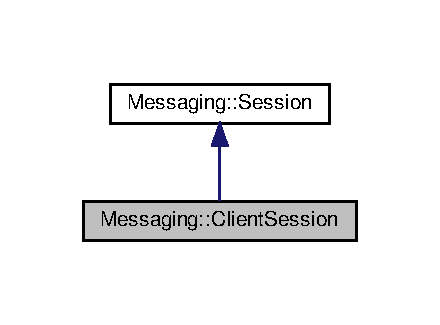
\includegraphics[width=211pt]{class_messaging_1_1_client_session__inherit__graph}
\end{center}
\end{figure}


Collaboration diagram for Messaging\+:\+:Client\+Session\+:
\nopagebreak
\begin{figure}[H]
\begin{center}
\leavevmode
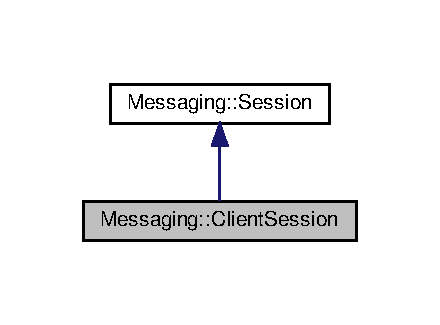
\includegraphics[width=211pt]{class_messaging_1_1_client_session__coll__graph}
\end{center}
\end{figure}
\subsection*{Public Member Functions}
\begin{DoxyCompactItemize}
\item 
\hyperlink{class_messaging_1_1_client_session_adad9b3dc7dfa45237cb53784f1710906}{Client\+Session} (\hyperlink{struct_messaging_1_1_message}{Message} a\+Message, boost\+::asio\+::io\+\_\+service \&io\+\_\+service, Response\+Handler\+Ptr a\+Response\+Handler)
\item 
virtual void \hyperlink{class_messaging_1_1_client_session_abdafb1626e9eb590ae2ed984e095a490}{start} ()
\item 
virtual void \hyperlink{class_messaging_1_1_client_session_a0539a7c332de1b853fd3405ac23b696c}{handle\+Message\+Read} (\hyperlink{struct_messaging_1_1_message}{Message} \&a\+Message)
\item 
virtual void \hyperlink{class_messaging_1_1_client_session_a9bfa2e2edfe325487ee04b046fdc4604}{handle\+Message\+Written} (\hyperlink{struct_messaging_1_1_message}{Message} \&U\+N\+U\+S\+E\+D\+P\+A\+R\+AM(a\+Message))
\end{DoxyCompactItemize}
\subsection*{Additional Inherited Members}


\subsection{Constructor \& Destructor Documentation}
\index{Messaging\+::\+Client\+Session@{Messaging\+::\+Client\+Session}!Client\+Session@{Client\+Session}}
\index{Client\+Session@{Client\+Session}!Messaging\+::\+Client\+Session@{Messaging\+::\+Client\+Session}}
\subsubsection[{\texorpdfstring{Client\+Session(\+Message a\+Message, boost\+::asio\+::io\+\_\+service \&io\+\_\+service, Response\+Handler\+Ptr a\+Response\+Handler)}{ClientSession(Message aMessage, boost::asio::io_service &io_service, ResponseHandlerPtr aResponseHandler)}}]{\setlength{\rightskip}{0pt plus 5cm}Messaging\+::\+Client\+Session\+::\+Client\+Session (
\begin{DoxyParamCaption}
\item[{{\bf Message}}]{a\+Message, }
\item[{boost\+::asio\+::io\+\_\+service \&}]{io\+\_\+service, }
\item[{Response\+Handler\+Ptr}]{a\+Response\+Handler}
\end{DoxyParamCaption}
)\hspace{0.3cm}{\ttfamily [inline]}}\hypertarget{class_messaging_1_1_client_session_adad9b3dc7dfa45237cb53784f1710906}{}\label{class_messaging_1_1_client_session_adad9b3dc7dfa45237cb53784f1710906}

\begin{DoxyParams}{Parameters}
{\em a\+Message} & \\
\hline
{\em io\+\_\+service} & \\
\hline
{\em a\+Response\+Handler} & \\
\hline
\end{DoxyParams}


\subsection{Member Function Documentation}
\index{Messaging\+::\+Client\+Session@{Messaging\+::\+Client\+Session}!handle\+Message\+Read@{handle\+Message\+Read}}
\index{handle\+Message\+Read@{handle\+Message\+Read}!Messaging\+::\+Client\+Session@{Messaging\+::\+Client\+Session}}
\subsubsection[{\texorpdfstring{handle\+Message\+Read(\+Message \&a\+Message)}{handleMessageRead(Message &aMessage)}}]{\setlength{\rightskip}{0pt plus 5cm}virtual void Messaging\+::\+Client\+Session\+::handle\+Message\+Read (
\begin{DoxyParamCaption}
\item[{{\bf Message} \&}]{a\+Message}
\end{DoxyParamCaption}
)\hspace{0.3cm}{\ttfamily [inline]}, {\ttfamily [virtual]}}\hypertarget{class_messaging_1_1_client_session_a0539a7c332de1b853fd3405ac23b696c}{}\label{class_messaging_1_1_client_session_a0539a7c332de1b853fd3405ac23b696c}
\begin{DoxySeeAlso}{See also}
\hyperlink{class_messaging_1_1_session_ac2fbf589586288cee9b408514907d044}{Session\+::handle\+Message\+Read( Message\& a\+Message)} 
\end{DoxySeeAlso}


Implements \hyperlink{class_messaging_1_1_session_ac2fbf589586288cee9b408514907d044}{Messaging\+::\+Session}.

\index{Messaging\+::\+Client\+Session@{Messaging\+::\+Client\+Session}!handle\+Message\+Written@{handle\+Message\+Written}}
\index{handle\+Message\+Written@{handle\+Message\+Written}!Messaging\+::\+Client\+Session@{Messaging\+::\+Client\+Session}}
\subsubsection[{\texorpdfstring{handle\+Message\+Written(\+Message \&\+U\+N\+U\+S\+E\+D\+P\+A\+R\+A\+M(a\+Message))}{handleMessageWritten(Message &UNUSEDPARAM(aMessage))}}]{\setlength{\rightskip}{0pt plus 5cm}virtual void Messaging\+::\+Client\+Session\+::handle\+Message\+Written (
\begin{DoxyParamCaption}
\item[{{\bf Message} \&}]{U\+N\+U\+S\+E\+D\+P\+A\+R\+AMa\+Message}
\end{DoxyParamCaption}
)\hspace{0.3cm}{\ttfamily [inline]}, {\ttfamily [virtual]}}\hypertarget{class_messaging_1_1_client_session_a9bfa2e2edfe325487ee04b046fdc4604}{}\label{class_messaging_1_1_client_session_a9bfa2e2edfe325487ee04b046fdc4604}
\begin{DoxySeeAlso}{See also}
\hyperlink{class_messaging_1_1_session_afcf204df8f7e67e470d454d9de561515}{Session\+::handle\+Message\+Written( Message\& a\+Message)} 
\end{DoxySeeAlso}
\index{Messaging\+::\+Client\+Session@{Messaging\+::\+Client\+Session}!start@{start}}
\index{start@{start}!Messaging\+::\+Client\+Session@{Messaging\+::\+Client\+Session}}
\subsubsection[{\texorpdfstring{start()}{start()}}]{\setlength{\rightskip}{0pt plus 5cm}virtual void Messaging\+::\+Client\+Session\+::start (
\begin{DoxyParamCaption}
{}
\end{DoxyParamCaption}
)\hspace{0.3cm}{\ttfamily [inline]}, {\ttfamily [virtual]}}\hypertarget{class_messaging_1_1_client_session_abdafb1626e9eb590ae2ed984e095a490}{}\label{class_messaging_1_1_client_session_abdafb1626e9eb590ae2ed984e095a490}
\begin{DoxySeeAlso}{See also}
\hyperlink{class_messaging_1_1_session_a89cbd6e05fdbbe1c9e26cbcab92d6044}{Session\+::start()} 
\end{DoxySeeAlso}


Implements \hyperlink{class_messaging_1_1_session_a89cbd6e05fdbbe1c9e26cbcab92d6044}{Messaging\+::\+Session}.



The documentation for this class was generated from the following file\+:\begin{DoxyCompactItemize}
\item 
/home/hqnders/\+Documents/robotworld/src/Session.\+hpp\end{DoxyCompactItemize}

\hypertarget{class_application_1_1_commandline_argument}{}\section{Application\+:\+:Commandline\+Argument Class Reference}
\label{class_application_1_1_commandline_argument}\index{Application\+::\+Commandline\+Argument@{Application\+::\+Commandline\+Argument}}


{\ttfamily \#include $<$Commandline\+Argument.\+hpp$>$}

\subsection*{Public Member Functions}
\begin{Indent}{\bf Constructors and destructor}\par
\begin{DoxyCompactItemize}
\item 
{\bfseries Commandline\+Argument} ()\hypertarget{class_application_1_1_commandline_argument_a8d1a860e8afe53e8b6f05e9f2dd4dce7}{}\label{class_application_1_1_commandline_argument_a8d1a860e8afe53e8b6f05e9f2dd4dce7}

\item 
\hyperlink{class_application_1_1_commandline_argument_a0bfdc3e855d3eda7c231d7e6c49cf0ef}{Commandline\+Argument} (unsigned long an\+Argument\+Number, const std\+::string \&a\+Variable, const std\+::string \&a\+Value)
\item 
\hyperlink{class_application_1_1_commandline_argument_a9f540c035645fc326ffd8d25fb6dce47}{Commandline\+Argument} (const \hyperlink{class_application_1_1_commandline_argument}{Commandline\+Argument} \&a\+Commandline\+Argument)
\item 
virtual {\bfseries $\sim$\+Commandline\+Argument} ()\hypertarget{class_application_1_1_commandline_argument_abfce42a49b80cb1c67d86bef4f0ac149}{}\label{class_application_1_1_commandline_argument_abfce42a49b80cb1c67d86bef4f0ac149}

\end{DoxyCompactItemize}
\end{Indent}
\begin{Indent}{\bf Operators}\par
\begin{DoxyCompactItemize}
\item 
\hyperlink{class_application_1_1_commandline_argument}{Commandline\+Argument} \& {\bfseries operator=} (const \hyperlink{class_application_1_1_commandline_argument}{Commandline\+Argument} \&a\+Commandline\+Argument)\hypertarget{class_application_1_1_commandline_argument_ae25c8fc78be1916eb7f1d318bcafb522}{}\label{class_application_1_1_commandline_argument_ae25c8fc78be1916eb7f1d318bcafb522}

\item 
bool {\bfseries operator==} (const unsigned long an\+Argument\+Number) const \hypertarget{class_application_1_1_commandline_argument_a1c091987640031464672fa515f697d3c}{}\label{class_application_1_1_commandline_argument_a1c091987640031464672fa515f697d3c}

\item 
bool {\bfseries operator==} (const std\+::string \&a\+Variable) const \hypertarget{class_application_1_1_commandline_argument_afba9475a894dd299642db8d7f040a0bf}{}\label{class_application_1_1_commandline_argument_afba9475a894dd299642db8d7f040a0bf}

\item 
bool {\bfseries operator==} (const \hyperlink{class_application_1_1_commandline_argument}{Commandline\+Argument} \&a\+Commandline\+Argument) const \hypertarget{class_application_1_1_commandline_argument_a1e4be92ec312c792b41aab43c4e5bbc5}{}\label{class_application_1_1_commandline_argument_a1e4be92ec312c792b41aab43c4e5bbc5}

\item 
bool \hyperlink{class_application_1_1_commandline_argument_a0359940fe4dae2674f7a59525809db60}{operator$<$} (const \hyperlink{class_application_1_1_commandline_argument}{Commandline\+Argument} \&a\+Commandline\+Argument) const 
\end{DoxyCompactItemize}
\end{Indent}
\subsection*{Public Attributes}
\begin{DoxyCompactItemize}
\item 
unsigned long {\bfseries argument\+Number}\hypertarget{class_application_1_1_commandline_argument_a64fd7701d510bb51ab7403ea78ef0675}{}\label{class_application_1_1_commandline_argument_a64fd7701d510bb51ab7403ea78ef0675}

\item 
std\+::string {\bfseries variable}\hypertarget{class_application_1_1_commandline_argument_a262d2d8b034f4deb153699354aad1cf0}{}\label{class_application_1_1_commandline_argument_a262d2d8b034f4deb153699354aad1cf0}

\item 
std\+::string {\bfseries value}\hypertarget{class_application_1_1_commandline_argument_a723dac454adb5d224dcf3d5105d66abe}{}\label{class_application_1_1_commandline_argument_a723dac454adb5d224dcf3d5105d66abe}

\end{DoxyCompactItemize}


\subsection{Detailed Description}
The \hyperlink{class_application_1_1_commandline_argument}{Commandline\+Argument} class encapsulates any command line argument given to the application 

\subsection{Constructor \& Destructor Documentation}
\index{Application\+::\+Commandline\+Argument@{Application\+::\+Commandline\+Argument}!Commandline\+Argument@{Commandline\+Argument}}
\index{Commandline\+Argument@{Commandline\+Argument}!Application\+::\+Commandline\+Argument@{Application\+::\+Commandline\+Argument}}
\subsubsection[{\texorpdfstring{Commandline\+Argument(unsigned long an\+Argument\+Number, const std\+::string \&a\+Variable, const std\+::string \&a\+Value)}{CommandlineArgument(unsigned long anArgumentNumber, const std::string &aVariable, const std::string &aValue)}}]{\setlength{\rightskip}{0pt plus 5cm}Application\+::\+Commandline\+Argument\+::\+Commandline\+Argument (
\begin{DoxyParamCaption}
\item[{unsigned long}]{an\+Argument\+Number, }
\item[{const std\+::string \&}]{a\+Variable, }
\item[{const std\+::string \&}]{a\+Value}
\end{DoxyParamCaption}
)\hspace{0.3cm}{\ttfamily [inline]}}\hypertarget{class_application_1_1_commandline_argument_a0bfdc3e855d3eda7c231d7e6c49cf0ef}{}\label{class_application_1_1_commandline_argument_a0bfdc3e855d3eda7c231d7e6c49cf0ef}

\begin{DoxyParams}{Parameters}
{\em an\+Argument\+Number} & \\
\hline
{\em a\+Variable} & \\
\hline
{\em a\+Value} & \\
\hline
\end{DoxyParams}
\index{Application\+::\+Commandline\+Argument@{Application\+::\+Commandline\+Argument}!Commandline\+Argument@{Commandline\+Argument}}
\index{Commandline\+Argument@{Commandline\+Argument}!Application\+::\+Commandline\+Argument@{Application\+::\+Commandline\+Argument}}
\subsubsection[{\texorpdfstring{Commandline\+Argument(const Commandline\+Argument \&a\+Commandline\+Argument)}{CommandlineArgument(const CommandlineArgument &aCommandlineArgument)}}]{\setlength{\rightskip}{0pt plus 5cm}Application\+::\+Commandline\+Argument\+::\+Commandline\+Argument (
\begin{DoxyParamCaption}
\item[{const {\bf Commandline\+Argument} \&}]{a\+Commandline\+Argument}
\end{DoxyParamCaption}
)\hspace{0.3cm}{\ttfamily [inline]}}\hypertarget{class_application_1_1_commandline_argument_a9f540c035645fc326ffd8d25fb6dce47}{}\label{class_application_1_1_commandline_argument_a9f540c035645fc326ffd8d25fb6dce47}

\begin{DoxyParams}{Parameters}
{\em a\+Commandline\+Argument} & \\
\hline
\end{DoxyParams}


\subsection{Member Function Documentation}
\index{Application\+::\+Commandline\+Argument@{Application\+::\+Commandline\+Argument}!operator$<$@{operator$<$}}
\index{operator$<$@{operator$<$}!Application\+::\+Commandline\+Argument@{Application\+::\+Commandline\+Argument}}
\subsubsection[{\texorpdfstring{operator$<$(const Commandline\+Argument \&a\+Commandline\+Argument) const }{operator<(const CommandlineArgument &aCommandlineArgument) const }}]{\setlength{\rightskip}{0pt plus 5cm}bool Application\+::\+Commandline\+Argument\+::operator$<$ (
\begin{DoxyParamCaption}
\item[{const {\bf Commandline\+Argument} \&}]{a\+Commandline\+Argument}
\end{DoxyParamCaption}
) const\hspace{0.3cm}{\ttfamily [inline]}}\hypertarget{class_application_1_1_commandline_argument_a0359940fe4dae2674f7a59525809db60}{}\label{class_application_1_1_commandline_argument_a0359940fe4dae2674f7a59525809db60}
Only compares the argument number. 

The documentation for this class was generated from the following file\+:\begin{DoxyCompactItemize}
\item 
/home/hqnders/\+Documents/robotworld/src/Commandline\+Argument.\+hpp\end{DoxyCompactItemize}

\hypertarget{class_messaging_1_1_communication_service}{}\section{Messaging\+:\+:Communication\+Service Class Reference}
\label{class_messaging_1_1_communication_service}\index{Messaging\+::\+Communication\+Service@{Messaging\+::\+Communication\+Service}}
\subsection*{Public Member Functions}
\begin{DoxyCompactItemize}
\item 
boost\+::asio\+::io\+\_\+service \& \hyperlink{class_messaging_1_1_communication_service_a603bfa697fbac1d8ea95115fbc78de24}{get\+I\+O\+Service} ()
\item 
void \hyperlink{class_messaging_1_1_communication_service_a91ea43508fc513e2be07071314bfcad9}{run\+Request\+Handler} (Request\+Handler\+Ptr a\+Request\+Handler, short a\+Port=12345)
\item 
void \hyperlink{class_messaging_1_1_communication_service_aafbba827051d66b74a0d5262074a950a}{run\+Request\+Handler} (Request\+Handler\+Ptr a\+Request\+Handler, const std\+::string \&a\+Port)
\end{DoxyCompactItemize}
\subsection*{Static Public Member Functions}
\begin{DoxyCompactItemize}
\item 
static \hyperlink{class_messaging_1_1_communication_service}{Communication\+Service} \& {\bfseries get\+Communication\+Service} ()\hypertarget{class_messaging_1_1_communication_service_a84eb6ffc757597611e01dfacb46c3702}{}\label{class_messaging_1_1_communication_service_a84eb6ffc757597611e01dfacb46c3702}

\end{DoxyCompactItemize}


\subsection{Member Function Documentation}
\index{Messaging\+::\+Communication\+Service@{Messaging\+::\+Communication\+Service}!get\+I\+O\+Service@{get\+I\+O\+Service}}
\index{get\+I\+O\+Service@{get\+I\+O\+Service}!Messaging\+::\+Communication\+Service@{Messaging\+::\+Communication\+Service}}
\subsubsection[{\texorpdfstring{get\+I\+O\+Service()}{getIOService()}}]{\setlength{\rightskip}{0pt plus 5cm}boost\+::asio\+::io\+\_\+service \& Messaging\+::\+Communication\+Service\+::get\+I\+O\+Service (
\begin{DoxyParamCaption}
{}
\end{DoxyParamCaption}
)}\hypertarget{class_messaging_1_1_communication_service_a603bfa697fbac1d8ea95115fbc78de24}{}\label{class_messaging_1_1_communication_service_a603bfa697fbac1d8ea95115fbc78de24}
This function is public because otherwise it the classes \hyperlink{class_messaging_1_1_session}{Session}, \hyperlink{class_messaging_1_1_server}{Server} and \hyperlink{class_messaging_1_1_client}{Client} have to be friends \index{Messaging\+::\+Communication\+Service@{Messaging\+::\+Communication\+Service}!run\+Request\+Handler@{run\+Request\+Handler}}
\index{run\+Request\+Handler@{run\+Request\+Handler}!Messaging\+::\+Communication\+Service@{Messaging\+::\+Communication\+Service}}
\subsubsection[{\texorpdfstring{run\+Request\+Handler(\+Request\+Handler\+Ptr a\+Request\+Handler, short a\+Port=12345)}{runRequestHandler(RequestHandlerPtr aRequestHandler, short aPort=12345)}}]{\setlength{\rightskip}{0pt plus 5cm}void Messaging\+::\+Communication\+Service\+::run\+Request\+Handler (
\begin{DoxyParamCaption}
\item[{Request\+Handler\+Ptr}]{a\+Request\+Handler, }
\item[{short}]{a\+Port = {\ttfamily 12345}}
\end{DoxyParamCaption}
)}\hypertarget{class_messaging_1_1_communication_service_a91ea43508fc513e2be07071314bfcad9}{}\label{class_messaging_1_1_communication_service_a91ea43508fc513e2be07071314bfcad9}
Runs the given a\+Request\+Handler at the given port until boost\+::asio\+::io\+\_\+service\+::io\+\_\+service.\+run() returns. In the limited context of Robot\+World this is done by sending a \char`\"{}stop\char`\"{}-\/message. \begin{DoxySeeAlso}{See also}
\hyperlink{class_messaging_1_1_server_session_a294d16e8d6c8839fee2358443d78dc15}{Server\+Session\+::handle\+Message\+Read( Message\& a\+Message)} for the implementation. 
\end{DoxySeeAlso}
\index{Messaging\+::\+Communication\+Service@{Messaging\+::\+Communication\+Service}!run\+Request\+Handler@{run\+Request\+Handler}}
\index{run\+Request\+Handler@{run\+Request\+Handler}!Messaging\+::\+Communication\+Service@{Messaging\+::\+Communication\+Service}}
\subsubsection[{\texorpdfstring{run\+Request\+Handler(\+Request\+Handler\+Ptr a\+Request\+Handler, const std\+::string \&a\+Port)}{runRequestHandler(RequestHandlerPtr aRequestHandler, const std::string &aPort)}}]{\setlength{\rightskip}{0pt plus 5cm}void Messaging\+::\+Communication\+Service\+::run\+Request\+Handler (
\begin{DoxyParamCaption}
\item[{Request\+Handler\+Ptr}]{a\+Request\+Handler, }
\item[{const std\+::string \&}]{a\+Port}
\end{DoxyParamCaption}
)\hspace{0.3cm}{\ttfamily [inline]}}\hypertarget{class_messaging_1_1_communication_service_aafbba827051d66b74a0d5262074a950a}{}\label{class_messaging_1_1_communication_service_aafbba827051d66b74a0d5262074a950a}
Uses \hyperlink{namespacestd_a5a4884a3b1890357be19cd6ff56179da}{std\+::stoi} for string to {\itshape int} conversion. Throws the exceptions that \hyperlink{namespacestd_a5a4884a3b1890357be19cd6ff56179da}{std\+::stoi} may throw. If int $>$ max short you lose... 

The documentation for this class was generated from the following files\+:\begin{DoxyCompactItemize}
\item 
/home/hqnders/\+Documents/robotworld/src/Communication\+Service.\+hpp\item 
/home/hqnders/\+Documents/robotworld/src/Communication\+Service.\+cpp\end{DoxyCompactItemize}

\hypertarget{class_base_1_1_debug_trace_function}{}\section{Base\+:\+:Debug\+Trace\+Function Class Reference}
\label{class_base_1_1_debug_trace_function}\index{Base\+::\+Debug\+Trace\+Function@{Base\+::\+Debug\+Trace\+Function}}


Inheritance diagram for Base\+:\+:Debug\+Trace\+Function\+:
\nopagebreak
\begin{figure}[H]
\begin{center}
\leavevmode
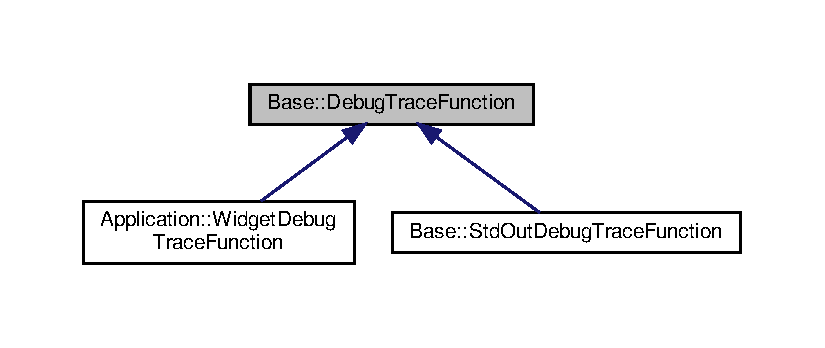
\includegraphics[width=350pt]{class_base_1_1_debug_trace_function__inherit__graph}
\end{center}
\end{figure}
\subsection*{Public Member Functions}
\begin{DoxyCompactItemize}
\item 
virtual \hyperlink{class_base_1_1_debug_trace_function_a10bd2fd587e2312ca418f594d33c3933}{$\sim$\+Debug\+Trace\+Function} ()
\item 
virtual void \hyperlink{class_base_1_1_debug_trace_function_a54f5a1f127e7624e50bb1a43146f8998}{trace} (const std\+::string \&a\+Text)=0
\end{DoxyCompactItemize}


\subsection{Constructor \& Destructor Documentation}
\index{Base\+::\+Debug\+Trace\+Function@{Base\+::\+Debug\+Trace\+Function}!````~Debug\+Trace\+Function@{$\sim$\+Debug\+Trace\+Function}}
\index{````~Debug\+Trace\+Function@{$\sim$\+Debug\+Trace\+Function}!Base\+::\+Debug\+Trace\+Function@{Base\+::\+Debug\+Trace\+Function}}
\subsubsection[{\texorpdfstring{$\sim$\+Debug\+Trace\+Function()}{~DebugTraceFunction()}}]{\setlength{\rightskip}{0pt plus 5cm}Base\+::\+Debug\+Trace\+Function\+::$\sim$\+Debug\+Trace\+Function (
\begin{DoxyParamCaption}
{}
\end{DoxyParamCaption}
)\hspace{0.3cm}{\ttfamily [virtual]}}\hypertarget{class_base_1_1_debug_trace_function_a10bd2fd587e2312ca418f594d33c3933}{}\label{class_base_1_1_debug_trace_function_a10bd2fd587e2312ca418f594d33c3933}
Virtual dtor as this is meant as a base class 

\subsection{Member Function Documentation}
\index{Base\+::\+Debug\+Trace\+Function@{Base\+::\+Debug\+Trace\+Function}!trace@{trace}}
\index{trace@{trace}!Base\+::\+Debug\+Trace\+Function@{Base\+::\+Debug\+Trace\+Function}}
\subsubsection[{\texorpdfstring{trace(const std\+::string \&a\+Text)=0}{trace(const std::string &aText)=0}}]{\setlength{\rightskip}{0pt plus 5cm}virtual void Base\+::\+Debug\+Trace\+Function\+::trace (
\begin{DoxyParamCaption}
\item[{const std\+::string \&}]{a\+Text}
\end{DoxyParamCaption}
)\hspace{0.3cm}{\ttfamily [pure virtual]}}\hypertarget{class_base_1_1_debug_trace_function_a54f5a1f127e7624e50bb1a43146f8998}{}\label{class_base_1_1_debug_trace_function_a54f5a1f127e7624e50bb1a43146f8998}

\begin{DoxyParams}{Parameters}
{\em a\+Text} & The text that will be send to the final trace destination. \\
\hline
\end{DoxyParams}


Implemented in \hyperlink{class_application_1_1_widget_debug_trace_function_ad4bf02cb1270957ff75fd07fe6b7f678}{Application\+::\+Widget\+Debug\+Trace\+Function}, and \hyperlink{class_base_1_1_std_out_debug_trace_function_a28cdac2a99589f238350d78743b920be}{Base\+::\+Std\+Out\+Debug\+Trace\+Function}.



The documentation for this class was generated from the following files\+:\begin{DoxyCompactItemize}
\item 
/home/hqnders/\+Documents/robotworld/src/Debug\+Trace\+Function.\+hpp\item 
/home/hqnders/\+Documents/robotworld/src/Debug\+Trace\+Function.\+cpp\end{DoxyCompactItemize}

\hypertarget{class_model_1_1_distance_percept}{}\section{model\+:\+:Distance\+Percept Class Reference}
\label{class_model_1_1_distance_percept}\index{model\+::\+Distance\+Percept@{model\+::\+Distance\+Percept}}


Inheritance diagram for model\+:\+:Distance\+Percept\+:
\nopagebreak
\begin{figure}[H]
\begin{center}
\leavevmode
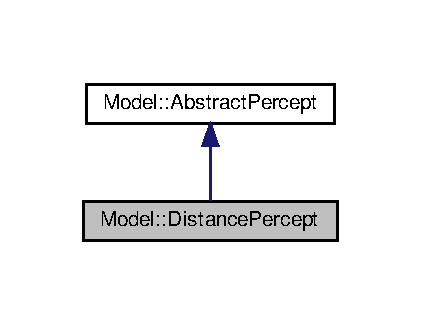
\includegraphics[width=202pt]{class_model_1_1_distance_percept__inherit__graph}
\end{center}
\end{figure}


Collaboration diagram for model\+:\+:Distance\+Percept\+:
\nopagebreak
\begin{figure}[H]
\begin{center}
\leavevmode
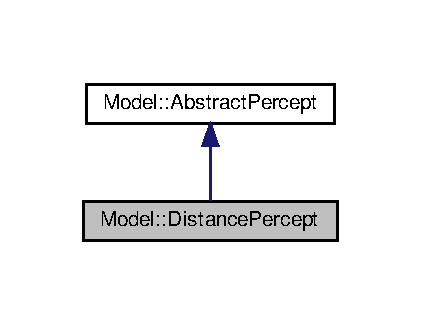
\includegraphics[width=202pt]{class_model_1_1_distance_percept__coll__graph}
\end{center}
\end{figure}
\subsection*{Public Member Functions}
\begin{DoxyCompactItemize}
\item 
{\bfseries Distance\+Percept} (const \hyperlink{class_model_1_1_distance_stimulus}{Distance\+Stimulus} \&a\+Distance\+Stimulus)\hypertarget{class_model_1_1_distance_percept_ab3cca9b4d5a5b837124688f9bab2e7f7}{}\label{class_model_1_1_distance_percept_ab3cca9b4d5a5b837124688f9bab2e7f7}

\item 
{\bfseries Distance\+Percept} (double an\+Angle, double a\+Distance)\hypertarget{class_model_1_1_distance_percept_a476417dd79dead365451b522d40a6995}{}\label{class_model_1_1_distance_percept_a476417dd79dead365451b522d40a6995}

\end{DoxyCompactItemize}
\subsection*{Public Attributes}
\begin{DoxyCompactItemize}
\item 
double {\bfseries angle}\hypertarget{class_model_1_1_distance_percept_a8e4a64e9c3844e42a211a0aa945f7998}{}\label{class_model_1_1_distance_percept_a8e4a64e9c3844e42a211a0aa945f7998}

\item 
double {\bfseries distance}\hypertarget{class_model_1_1_distance_percept_a83e7312e3ed47d97c6bfc41b9e0c0e4a}{}\label{class_model_1_1_distance_percept_a83e7312e3ed47d97c6bfc41b9e0c0e4a}

\end{DoxyCompactItemize}


The documentation for this class was generated from the following file\+:\begin{DoxyCompactItemize}
\item 
/home/hqnders/\+Documents/robotworld/src/Laser\+Distance\+Sensor.\+hpp\end{DoxyCompactItemize}

\hypertarget{class_model_1_1_distance_stimulus}{}\section{model\+:\+:Distance\+Stimulus Class Reference}
\label{class_model_1_1_distance_stimulus}\index{model\+::\+Distance\+Stimulus@{model\+::\+Distance\+Stimulus}}


Inheritance diagram for model\+:\+:Distance\+Stimulus\+:
\nopagebreak
\begin{figure}[H]
\begin{center}
\leavevmode
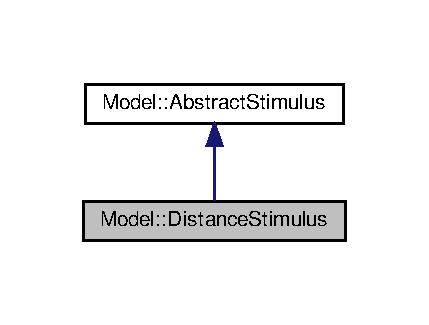
\includegraphics[width=206pt]{class_model_1_1_distance_stimulus__inherit__graph}
\end{center}
\end{figure}


Collaboration diagram for model\+:\+:Distance\+Stimulus\+:
\nopagebreak
\begin{figure}[H]
\begin{center}
\leavevmode
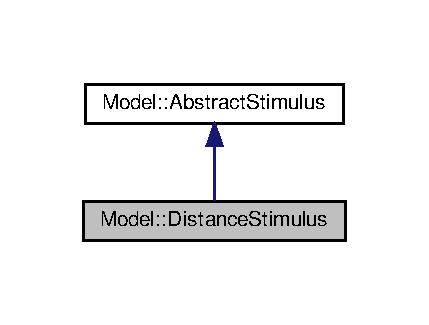
\includegraphics[width=206pt]{class_model_1_1_distance_stimulus__coll__graph}
\end{center}
\end{figure}
\subsection*{Public Member Functions}
\begin{DoxyCompactItemize}
\item 
{\bfseries Distance\+Stimulus} (double an\+Angle, double a\+Distance)\hypertarget{class_model_1_1_distance_stimulus_a5ec267e4e945106911cd9fff534e2b07}{}\label{class_model_1_1_distance_stimulus_a5ec267e4e945106911cd9fff534e2b07}

\end{DoxyCompactItemize}
\subsection*{Public Attributes}
\begin{DoxyCompactItemize}
\item 
double {\bfseries angle}\hypertarget{class_model_1_1_distance_stimulus_ac2a26e553ae72f4cdb28147cbac38bc4}{}\label{class_model_1_1_distance_stimulus_ac2a26e553ae72f4cdb28147cbac38bc4}

\item 
double {\bfseries distance}\hypertarget{class_model_1_1_distance_stimulus_a509312aa1c6cc55236a3b81014ea6d7c}{}\label{class_model_1_1_distance_stimulus_a509312aa1c6cc55236a3b81014ea6d7c}

\end{DoxyCompactItemize}


The documentation for this class was generated from the following file\+:\begin{DoxyCompactItemize}
\item 
/home/hqnders/\+Documents/robotworld/src/Laser\+Distance\+Sensor.\+hpp\end{DoxyCompactItemize}

\hypertarget{struct_path_algorithm_1_1_edge}{}\section{Path\+Algorithm\+:\+:Edge Struct Reference}
\label{struct_path_algorithm_1_1_edge}\index{Path\+Algorithm\+::\+Edge@{Path\+Algorithm\+::\+Edge}}


Collaboration diagram for Path\+Algorithm\+:\+:Edge\+:
\nopagebreak
\begin{figure}[H]
\begin{center}
\leavevmode
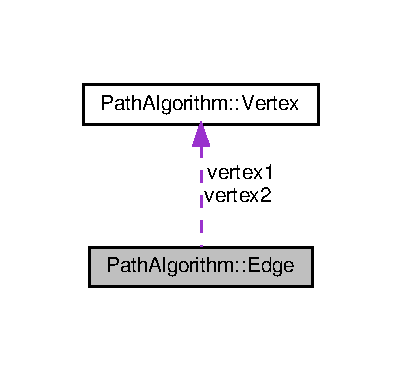
\includegraphics[width=193pt]{struct_path_algorithm_1_1_edge__coll__graph}
\end{center}
\end{figure}
\subsection*{Public Member Functions}
\begin{DoxyCompactItemize}
\item 
{\bfseries Edge} (const \hyperlink{struct_path_algorithm_1_1_vertex}{Vertex} \&a\+Vertex1, const \hyperlink{struct_path_algorithm_1_1_vertex}{Vertex} \&a\+Vertex2)\hypertarget{struct_path_algorithm_1_1_edge_a4378105bc5d8b8b2fd147cb8b5a62662}{}\label{struct_path_algorithm_1_1_edge_a4378105bc5d8b8b2fd147cb8b5a62662}

\item 
{\bfseries Edge} (const \hyperlink{struct_path_algorithm_1_1_edge}{Edge} \&an\+Edge)\hypertarget{struct_path_algorithm_1_1_edge_a2a1cfa63c51fac6e9c7385ab6b0b0b0c}{}\label{struct_path_algorithm_1_1_edge_a2a1cfa63c51fac6e9c7385ab6b0b0b0c}

\item 
const \hyperlink{struct_path_algorithm_1_1_vertex}{Vertex} \& {\bfseries this\+Side} (const \hyperlink{struct_path_algorithm_1_1_vertex}{Vertex} \&a\+Vertex) const \hypertarget{struct_path_algorithm_1_1_edge_a0a987c8705e5e41f890fb4f222243af8}{}\label{struct_path_algorithm_1_1_edge_a0a987c8705e5e41f890fb4f222243af8}

\item 
const \hyperlink{struct_path_algorithm_1_1_vertex}{Vertex} \& {\bfseries other\+Side} (const \hyperlink{struct_path_algorithm_1_1_vertex}{Vertex} \&a\+Vertex) const \hypertarget{struct_path_algorithm_1_1_edge_a204de7bc294af2cd5df73c29b2587345}{}\label{struct_path_algorithm_1_1_edge_a204de7bc294af2cd5df73c29b2587345}

\end{DoxyCompactItemize}
\subsection*{Public Attributes}
\begin{DoxyCompactItemize}
\item 
\hyperlink{struct_path_algorithm_1_1_vertex}{Vertex} {\bfseries vertex1}\hypertarget{struct_path_algorithm_1_1_edge_ab655d5ef6c7022bc87520c4e751b4dcf}{}\label{struct_path_algorithm_1_1_edge_ab655d5ef6c7022bc87520c4e751b4dcf}

\item 
\hyperlink{struct_path_algorithm_1_1_vertex}{Vertex} {\bfseries vertex2}\hypertarget{struct_path_algorithm_1_1_edge_ab8d28fabc8b10986f4e4d915f0b6f16a}{}\label{struct_path_algorithm_1_1_edge_ab8d28fabc8b10986f4e4d915f0b6f16a}

\end{DoxyCompactItemize}


The documentation for this struct was generated from the following file\+:\begin{DoxyCompactItemize}
\item 
/home/hqnders/\+Documents/robotworld/src/A\+Star.\+hpp\end{DoxyCompactItemize}

\hypertarget{class_model_1_1_goal}{}\section{model\+:\+:Goal Class Reference}
\label{class_model_1_1_goal}\index{model\+::\+Goal@{model\+::\+Goal}}


Inheritance diagram for model\+:\+:Goal\+:
\nopagebreak
\begin{figure}[H]
\begin{center}
\leavevmode
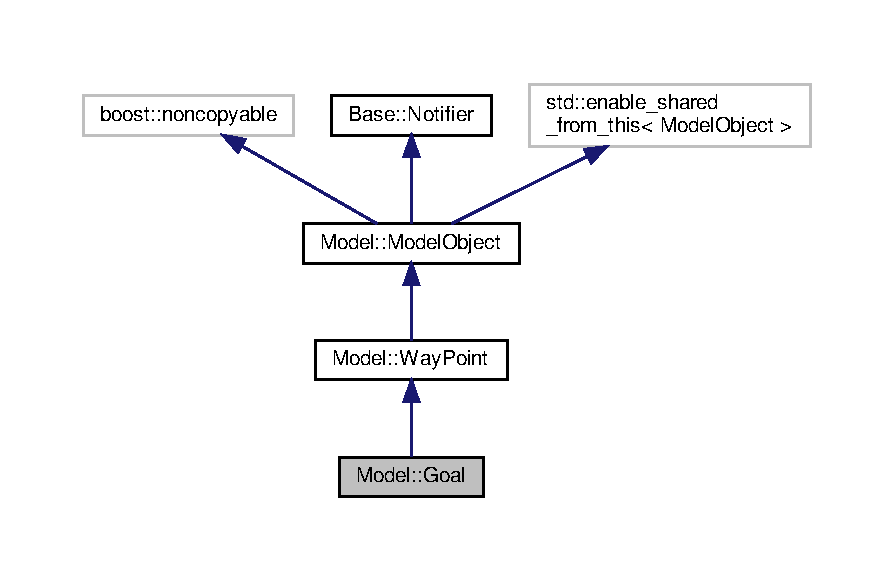
\includegraphics[width=350pt]{class_model_1_1_goal__inherit__graph}
\end{center}
\end{figure}


Collaboration diagram for model\+:\+:Goal\+:
\nopagebreak
\begin{figure}[H]
\begin{center}
\leavevmode
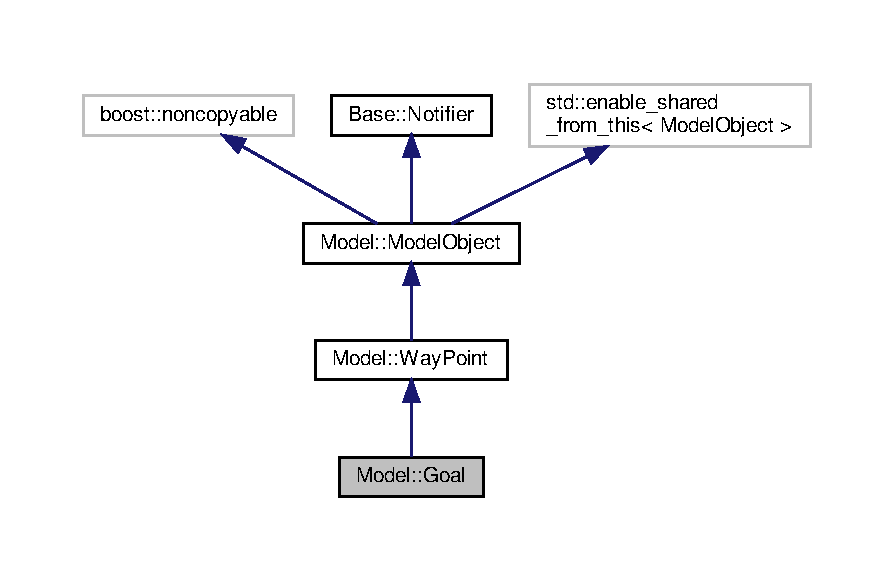
\includegraphics[width=350pt]{class_model_1_1_goal__coll__graph}
\end{center}
\end{figure}
\subsection*{Public Member Functions}
\begin{DoxyCompactItemize}
\item 
{\bfseries Goal} (const std\+::string \&a\+Name)\hypertarget{class_model_1_1_goal_a942dd4460b918de703e7a39723b310e4}{}\label{class_model_1_1_goal_a942dd4460b918de703e7a39723b310e4}

\item 
{\bfseries Goal} (const std\+::string \&a\+Name, const Point \&a\+Position)\hypertarget{class_model_1_1_goal_a04afed8db36d97690a46e764d0d56964}{}\label{class_model_1_1_goal_a04afed8db36d97690a46e764d0d56964}

\end{DoxyCompactItemize}
\begin{Indent}{\bf Debug functions}\par
\begin{DoxyCompactItemize}
\item 
virtual std\+::string \hyperlink{class_model_1_1_goal_a3a2482cbc274b38165125a75be970f29}{as\+String} () const 
\item 
virtual std\+::string \hyperlink{class_model_1_1_goal_a30c24f8dfe63a025222753f7d8fa8392}{as\+Debug\+String} () const 
\end{DoxyCompactItemize}
\end{Indent}


\subsection{Member Function Documentation}
\index{model\+::\+Goal@{model\+::\+Goal}!as\+Debug\+String@{as\+Debug\+String}}
\index{as\+Debug\+String@{as\+Debug\+String}!model\+::\+Goal@{model\+::\+Goal}}
\subsubsection[{\texorpdfstring{as\+Debug\+String() const }{asDebugString() const }}]{\setlength{\rightskip}{0pt plus 5cm}std\+::string model\+::\+Goal\+::as\+Debug\+String (
\begin{DoxyParamCaption}
{}
\end{DoxyParamCaption}
) const\hspace{0.3cm}{\ttfamily [virtual]}}\hypertarget{class_model_1_1_goal_a30c24f8dfe63a025222753f7d8fa8392}{}\label{class_model_1_1_goal_a30c24f8dfe63a025222753f7d8fa8392}
Returns a description of the object with all data of the object usable for debugging 

Reimplemented from \hyperlink{class_model_1_1_way_point_aa7acf33a786c98fa593a3a38d6270723}{model\+::\+Way\+Point}.

\index{model\+::\+Goal@{model\+::\+Goal}!as\+String@{as\+String}}
\index{as\+String@{as\+String}!model\+::\+Goal@{model\+::\+Goal}}
\subsubsection[{\texorpdfstring{as\+String() const }{asString() const }}]{\setlength{\rightskip}{0pt plus 5cm}std\+::string model\+::\+Goal\+::as\+String (
\begin{DoxyParamCaption}
{}
\end{DoxyParamCaption}
) const\hspace{0.3cm}{\ttfamily [virtual]}}\hypertarget{class_model_1_1_goal_a3a2482cbc274b38165125a75be970f29}{}\label{class_model_1_1_goal_a3a2482cbc274b38165125a75be970f29}
Returns a 1-\/line description of the object 

Reimplemented from \hyperlink{class_model_1_1_way_point_a2504ccca4e76765faaf91b85c1e0fb75}{model\+::\+Way\+Point}.



The documentation for this class was generated from the following files\+:\begin{DoxyCompactItemize}
\item 
/home/hqnders/\+Documents/robotworld/src/Goal.\+hpp\item 
/home/hqnders/\+Documents/robotworld/src/Goal.\+cpp\end{DoxyCompactItemize}

\hypertarget{class_view_1_1_goal_shape}{}\section{View\+:\+:Goal\+Shape Class Reference}
\label{class_view_1_1_goal_shape}\index{View\+::\+Goal\+Shape@{View\+::\+Goal\+Shape}}


Inheritance diagram for View\+:\+:Goal\+Shape\+:
\nopagebreak
\begin{figure}[H]
\begin{center}
\leavevmode
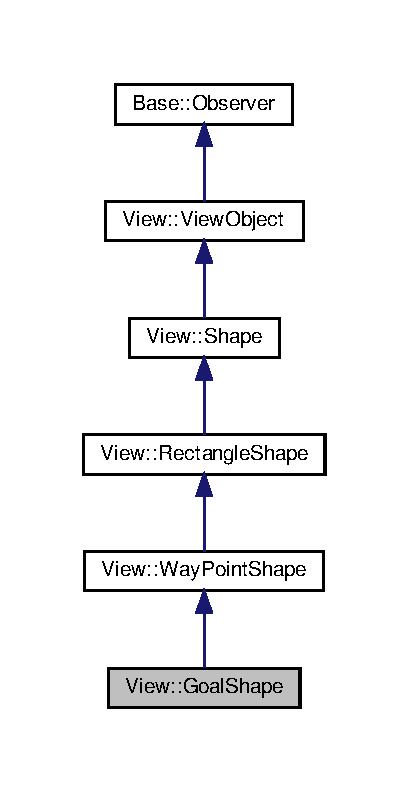
\includegraphics[width=196pt]{class_view_1_1_goal_shape__inherit__graph}
\end{center}
\end{figure}


Collaboration diagram for View\+:\+:Goal\+Shape\+:
\nopagebreak
\begin{figure}[H]
\begin{center}
\leavevmode
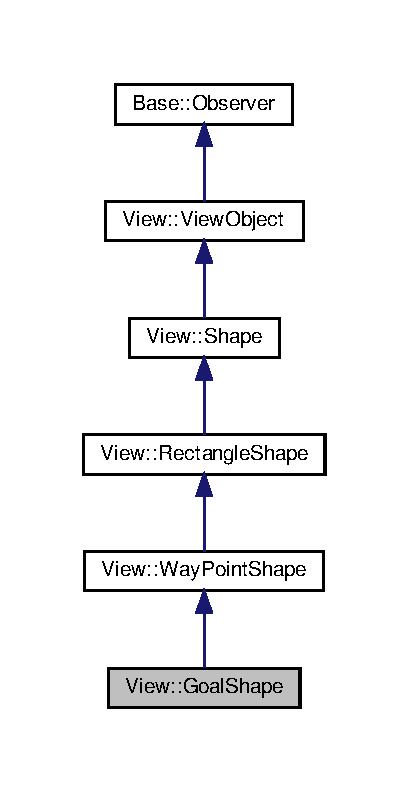
\includegraphics[width=196pt]{class_view_1_1_goal_shape__coll__graph}
\end{center}
\end{figure}
\subsection*{Public Member Functions}
\begin{DoxyCompactItemize}
\item 
{\bfseries Goal\+Shape} (model\+::\+Goal\+Ptr a\+Goal)\hypertarget{class_view_1_1_goal_shape_ac2dc0283bbdefcc5886f985f04611ffb}{}\label{class_view_1_1_goal_shape_ac2dc0283bbdefcc5886f985f04611ffb}

\item 
virtual std\+::string {\bfseries get\+Normal\+Colour} () const \hypertarget{class_view_1_1_goal_shape_a31a8bb188f7870024c168529e8788673}{}\label{class_view_1_1_goal_shape_a31a8bb188f7870024c168529e8788673}

\item 
virtual std\+::string {\bfseries get\+Selection\+Colour} () const \hypertarget{class_view_1_1_goal_shape_a9b0b0c7aa41bfe75723e847a4a57173e}{}\label{class_view_1_1_goal_shape_a9b0b0c7aa41bfe75723e847a4a57173e}

\item 
virtual std\+::string {\bfseries get\+Activation\+Colour} () const \hypertarget{class_view_1_1_goal_shape_a5f3f650fd43dc5ba30518deec6859506}{}\label{class_view_1_1_goal_shape_a5f3f650fd43dc5ba30518deec6859506}

\end{DoxyCompactItemize}
\begin{Indent}{\bf Type safe accessors and mutators}\par
\begin{DoxyCompactItemize}
\item 
model\+::\+Goal\+Ptr \hyperlink{class_view_1_1_goal_shape_a8c0c1cce167a4e8a0cf085f676c213a0}{get\+Goal} () const
\item 
void \hyperlink{class_view_1_1_goal_shape_a2e8149d939f204e0cc0efc2488af8fb2}{set\+Goal} (model\+::\+Goal\+Ptr a\+Goal)
\end{DoxyCompactItemize}
\end{Indent}
\begin{Indent}{\bf Observer functions}\par
\begin{DoxyCompactItemize}
\item 
virtual void \hyperlink{class_view_1_1_goal_shape_a881cfbfd4b3d6d3b37498e12d8291f6f}{handle\+Notification} ()
\end{DoxyCompactItemize}
\end{Indent}
\begin{Indent}{\bf Debug functions}\par
\begin{DoxyCompactItemize}
\item 
virtual std\+::string \hyperlink{class_view_1_1_goal_shape_a7f6c2c9c9502d264657a0b688e3d5e86}{as\+String} () const 
\item 
virtual std\+::string \hyperlink{class_view_1_1_goal_shape_a7d88c0780ae52278bacb44f4a6c79da5}{as\+Debug\+String} () const 
\end{DoxyCompactItemize}
\end{Indent}
\subsection*{Additional Inherited Members}


\subsection{Member Function Documentation}
\index{View\+::\+Goal\+Shape@{View\+::\+Goal\+Shape}!as\+Debug\+String@{as\+Debug\+String}}
\index{as\+Debug\+String@{as\+Debug\+String}!View\+::\+Goal\+Shape@{View\+::\+Goal\+Shape}}
\subsubsection[{\texorpdfstring{as\+Debug\+String() const }{asDebugString() const }}]{\setlength{\rightskip}{0pt plus 5cm}std\+::string View\+::\+Goal\+Shape\+::as\+Debug\+String (
\begin{DoxyParamCaption}
{}
\end{DoxyParamCaption}
) const\hspace{0.3cm}{\ttfamily [virtual]}}\hypertarget{class_view_1_1_goal_shape_a7d88c0780ae52278bacb44f4a6c79da5}{}\label{class_view_1_1_goal_shape_a7d88c0780ae52278bacb44f4a6c79da5}
Returns a description of the object with all data of the object usable for debugging 

Reimplemented from \hyperlink{class_view_1_1_way_point_shape_a0f21e281b69fe62eb8728ad5dc28fce6}{View\+::\+Way\+Point\+Shape}.

\index{View\+::\+Goal\+Shape@{View\+::\+Goal\+Shape}!as\+String@{as\+String}}
\index{as\+String@{as\+String}!View\+::\+Goal\+Shape@{View\+::\+Goal\+Shape}}
\subsubsection[{\texorpdfstring{as\+String() const }{asString() const }}]{\setlength{\rightskip}{0pt plus 5cm}std\+::string View\+::\+Goal\+Shape\+::as\+String (
\begin{DoxyParamCaption}
{}
\end{DoxyParamCaption}
) const\hspace{0.3cm}{\ttfamily [virtual]}}\hypertarget{class_view_1_1_goal_shape_a7f6c2c9c9502d264657a0b688e3d5e86}{}\label{class_view_1_1_goal_shape_a7f6c2c9c9502d264657a0b688e3d5e86}
Returns a 1-\/line description of the object 

Reimplemented from \hyperlink{class_view_1_1_way_point_shape_a89bbc1a878732d81245c5b5b6c5f035a}{View\+::\+Way\+Point\+Shape}.

\index{View\+::\+Goal\+Shape@{View\+::\+Goal\+Shape}!get\+Goal@{get\+Goal}}
\index{get\+Goal@{get\+Goal}!View\+::\+Goal\+Shape@{View\+::\+Goal\+Shape}}
\subsubsection[{\texorpdfstring{get\+Goal() const }{getGoal() const }}]{\setlength{\rightskip}{0pt plus 5cm}model\+::\+Goal\+Ptr View\+::\+Goal\+Shape\+::get\+Goal (
\begin{DoxyParamCaption}
{}
\end{DoxyParamCaption}
) const}\hypertarget{class_view_1_1_goal_shape_a8c0c1cce167a4e8a0cf085f676c213a0}{}\label{class_view_1_1_goal_shape_a8c0c1cce167a4e8a0cf085f676c213a0}
Type safe accessor \index{View\+::\+Goal\+Shape@{View\+::\+Goal\+Shape}!handle\+Notification@{handle\+Notification}}
\index{handle\+Notification@{handle\+Notification}!View\+::\+Goal\+Shape@{View\+::\+Goal\+Shape}}
\subsubsection[{\texorpdfstring{handle\+Notification()}{handleNotification()}}]{\setlength{\rightskip}{0pt plus 5cm}void View\+::\+Goal\+Shape\+::handle\+Notification (
\begin{DoxyParamCaption}
{}
\end{DoxyParamCaption}
)\hspace{0.3cm}{\ttfamily [virtual]}}\hypertarget{class_view_1_1_goal_shape_a881cfbfd4b3d6d3b37498e12d8291f6f}{}\label{class_view_1_1_goal_shape_a881cfbfd4b3d6d3b37498e12d8291f6f}
A Notifier will call this function if this Observer will handle the notifications of that Notifier. It is the responsibility of the Observer to filter any events it is interested in. 

Reimplemented from \hyperlink{class_view_1_1_way_point_shape_a84f786f8027e91441c8197cdb56b3d5f}{View\+::\+Way\+Point\+Shape}.

\index{View\+::\+Goal\+Shape@{View\+::\+Goal\+Shape}!set\+Goal@{set\+Goal}}
\index{set\+Goal@{set\+Goal}!View\+::\+Goal\+Shape@{View\+::\+Goal\+Shape}}
\subsubsection[{\texorpdfstring{set\+Goal(\+model\+::\+Goal\+Ptr a\+Goal)}{setGoal(model::GoalPtr aGoal)}}]{\setlength{\rightskip}{0pt plus 5cm}void View\+::\+Goal\+Shape\+::set\+Goal (
\begin{DoxyParamCaption}
\item[{model\+::\+Goal\+Ptr}]{a\+Goal}
\end{DoxyParamCaption}
)}\hypertarget{class_view_1_1_goal_shape_a2e8149d939f204e0cc0efc2488af8fb2}{}\label{class_view_1_1_goal_shape_a2e8149d939f204e0cc0efc2488af8fb2}
Type safe mutator 

The documentation for this class was generated from the following files\+:\begin{DoxyCompactItemize}
\item 
/home/hqnders/\+Documents/robotworld/src/Goal\+Shape.\+hpp\item 
/home/hqnders/\+Documents/robotworld/src/Goal\+Shape.\+cpp\end{DoxyCompactItemize}

\hypertarget{class_model_1_1_laser_distance_sensor}{}\section{model\+:\+:Laser\+Distance\+Sensor Class Reference}
\label{class_model_1_1_laser_distance_sensor}\index{model\+::\+Laser\+Distance\+Sensor@{model\+::\+Laser\+Distance\+Sensor}}


Inheritance diagram for model\+:\+:Laser\+Distance\+Sensor\+:
\nopagebreak
\begin{figure}[H]
\begin{center}
\leavevmode
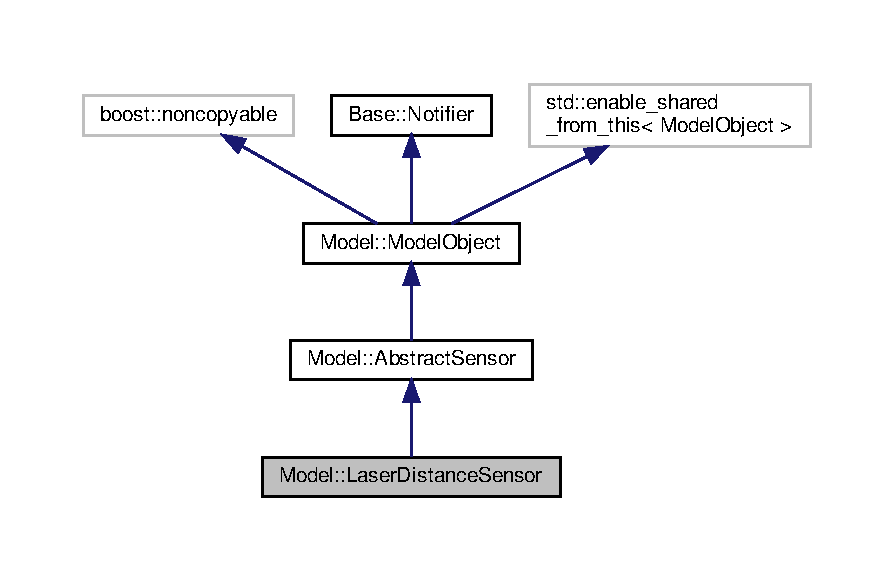
\includegraphics[width=350pt]{class_model_1_1_laser_distance_sensor__inherit__graph}
\end{center}
\end{figure}


Collaboration diagram for model\+:\+:Laser\+Distance\+Sensor\+:
\nopagebreak
\begin{figure}[H]
\begin{center}
\leavevmode
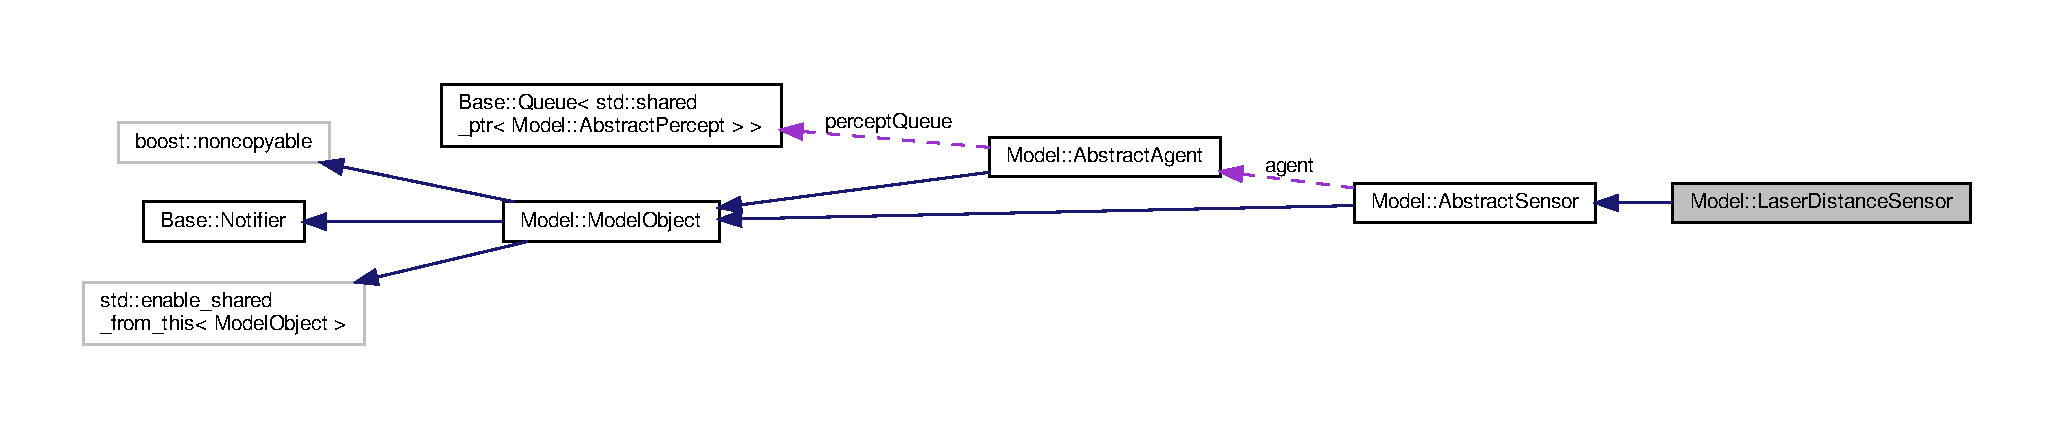
\includegraphics[width=350pt]{class_model_1_1_laser_distance_sensor__coll__graph}
\end{center}
\end{figure}
\subsection*{Public Member Functions}
\begin{DoxyCompactItemize}
\item 
{\bfseries Laser\+Distance\+Sensor} (\hyperlink{class_model_1_1_robot}{Robot} $\ast$a\+Robot)\hypertarget{class_model_1_1_laser_distance_sensor_aa9686c425108f245858bb281acf15346}{}\label{class_model_1_1_laser_distance_sensor_aa9686c425108f245858bb281acf15346}

\item 
virtual std\+::shared\+\_\+ptr$<$ \hyperlink{class_model_1_1_abstract_stimulus}{Abstract\+Stimulus} $>$ {\bfseries get\+Stimulus} () const \hypertarget{class_model_1_1_laser_distance_sensor_a532a168e8d0f7f6986075e83ba58de3e}{}\label{class_model_1_1_laser_distance_sensor_a532a168e8d0f7f6986075e83ba58de3e}

\item 
virtual std\+::shared\+\_\+ptr$<$ \hyperlink{class_model_1_1_abstract_percept}{Abstract\+Percept} $>$ {\bfseries get\+Percept\+For} (std\+::shared\+\_\+ptr$<$ \hyperlink{class_model_1_1_abstract_stimulus}{Abstract\+Stimulus} $>$ an\+Abstract\+Stimulus) const \hypertarget{class_model_1_1_laser_distance_sensor_af3dc2140292c2e3def32b89e3e0a5e87}{}\label{class_model_1_1_laser_distance_sensor_af3dc2140292c2e3def32b89e3e0a5e87}

\end{DoxyCompactItemize}
\begin{Indent}{\bf Debug functions}\par
\begin{DoxyCompactItemize}
\item 
virtual std\+::string \hyperlink{class_model_1_1_laser_distance_sensor_a9403593acd21d557e5af1d79901fde34}{as\+String} () const 
\item 
virtual std\+::string \hyperlink{class_model_1_1_laser_distance_sensor_ab32d7cbfd19a9a5ec12a0c06ebb02b4f}{as\+Debug\+String} () const 
\end{DoxyCompactItemize}
\end{Indent}
\subsection*{Additional Inherited Members}


\subsection{Member Function Documentation}
\index{model\+::\+Laser\+Distance\+Sensor@{model\+::\+Laser\+Distance\+Sensor}!as\+Debug\+String@{as\+Debug\+String}}
\index{as\+Debug\+String@{as\+Debug\+String}!model\+::\+Laser\+Distance\+Sensor@{model\+::\+Laser\+Distance\+Sensor}}
\subsubsection[{\texorpdfstring{as\+Debug\+String() const }{asDebugString() const }}]{\setlength{\rightskip}{0pt plus 5cm}std\+::string model\+::\+Laser\+Distance\+Sensor\+::as\+Debug\+String (
\begin{DoxyParamCaption}
{}
\end{DoxyParamCaption}
) const\hspace{0.3cm}{\ttfamily [virtual]}}\hypertarget{class_model_1_1_laser_distance_sensor_ab32d7cbfd19a9a5ec12a0c06ebb02b4f}{}\label{class_model_1_1_laser_distance_sensor_ab32d7cbfd19a9a5ec12a0c06ebb02b4f}
Returns a description of the object with all data of the object usable for debugging 

Reimplemented from \hyperlink{class_model_1_1_abstract_sensor_aa67bce32b6a602772773f0f23d0634f0}{model\+::\+Abstract\+Sensor}.

\index{model\+::\+Laser\+Distance\+Sensor@{model\+::\+Laser\+Distance\+Sensor}!as\+String@{as\+String}}
\index{as\+String@{as\+String}!model\+::\+Laser\+Distance\+Sensor@{model\+::\+Laser\+Distance\+Sensor}}
\subsubsection[{\texorpdfstring{as\+String() const }{asString() const }}]{\setlength{\rightskip}{0pt plus 5cm}std\+::string model\+::\+Laser\+Distance\+Sensor\+::as\+String (
\begin{DoxyParamCaption}
{}
\end{DoxyParamCaption}
) const\hspace{0.3cm}{\ttfamily [virtual]}}\hypertarget{class_model_1_1_laser_distance_sensor_a9403593acd21d557e5af1d79901fde34}{}\label{class_model_1_1_laser_distance_sensor_a9403593acd21d557e5af1d79901fde34}
Returns a 1-\/line description of the object 

Reimplemented from \hyperlink{class_model_1_1_abstract_sensor_a85c18d6d51b8b6a3b97f682ad242be9d}{model\+::\+Abstract\+Sensor}.



The documentation for this class was generated from the following files\+:\begin{DoxyCompactItemize}
\item 
/home/hqnders/\+Documents/robotworld/src/Laser\+Distance\+Sensor.\+hpp\item 
/home/hqnders/\+Documents/robotworld/src/Laser\+Distance\+Sensor.\+cpp\end{DoxyCompactItemize}

\hypertarget{class_view_1_1_line_shape}{}\section{View\+:\+:Line\+Shape Class Reference}
\label{class_view_1_1_line_shape}\index{View\+::\+Line\+Shape@{View\+::\+Line\+Shape}}


Inheritance diagram for View\+:\+:Line\+Shape\+:
\nopagebreak
\begin{figure}[H]
\begin{center}
\leavevmode
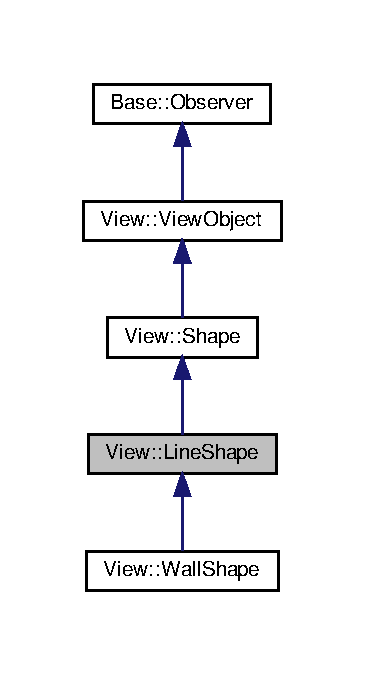
\includegraphics[width=175pt]{class_view_1_1_line_shape__inherit__graph}
\end{center}
\end{figure}


Collaboration diagram for View\+:\+:Line\+Shape\+:
\nopagebreak
\begin{figure}[H]
\begin{center}
\leavevmode
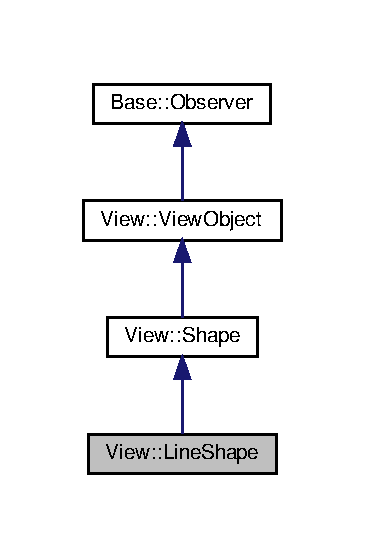
\includegraphics[width=175pt]{class_view_1_1_line_shape__coll__graph}
\end{center}
\end{figure}
\subsection*{Public Member Functions}
\begin{DoxyCompactItemize}
\item 
{\bfseries Line\+Shape} (Rectangle\+Shape\+Ptr a\+Node1, Rectangle\+Shape\+Ptr a\+Node2, const std\+::string \&a\+Title=\char`\"{}\char`\"{}, int a\+Line\+Width=1, int an\+Arrow\+Head\+Size=10)\hypertarget{class_view_1_1_line_shape_ab558c4ee9f3ee29a1b9bcee37e29354a}{}\label{class_view_1_1_line_shape_ab558c4ee9f3ee29a1b9bcee37e29354a}

\item 
{\bfseries Line\+Shape} (model\+::\+model\+Object\+Ptr a\+model\+Object, Rectangle\+Shape\+Ptr a\+Node1, Rectangle\+Shape\+Ptr a\+Node2, const std\+::string \&a\+Title=\char`\"{}\char`\"{}, int a\+Line\+Width=1, int an\+Arrow\+Head\+Size=10)\hypertarget{class_view_1_1_line_shape_a8f8bfaac1fb3f6925d7d3eb40f94d4c8}{}\label{class_view_1_1_line_shape_a8f8bfaac1fb3f6925d7d3eb40f94d4c8}

\item 
void {\bfseries draw\+Head} (wx\+DC \&dc)\hypertarget{class_view_1_1_line_shape_a2fe3effe9eff5bd00fe495e0f1c39606}{}\label{class_view_1_1_line_shape_a2fe3effe9eff5bd00fe495e0f1c39606}

\item 
std\+::string {\bfseries get\+Title} () const \hypertarget{class_view_1_1_line_shape_af83c7add92fbad90624d57dd3b7abc6a}{}\label{class_view_1_1_line_shape_af83c7add92fbad90624d57dd3b7abc6a}

\item 
void {\bfseries set\+Title} (const std\+::string \&a\+Title)\hypertarget{class_view_1_1_line_shape_a913834fd48496cc0bea586fcdcce86ad}{}\label{class_view_1_1_line_shape_a913834fd48496cc0bea586fcdcce86ad}

\item 
int {\bfseries get\+Line\+Width} () const \hypertarget{class_view_1_1_line_shape_a96e2e0cea7dc8dbbb82e22b538e324f3}{}\label{class_view_1_1_line_shape_a96e2e0cea7dc8dbbb82e22b538e324f3}

\item 
void {\bfseries set\+Line\+Width} (int a\+Line\+Width)\hypertarget{class_view_1_1_line_shape_a44f4b897aaaed84f5746898983d4da05}{}\label{class_view_1_1_line_shape_a44f4b897aaaed84f5746898983d4da05}

\item 
int {\bfseries get\+Arrow\+Head\+Size} () const \hypertarget{class_view_1_1_line_shape_a69e09bc46d6653c7569ec10495238cce}{}\label{class_view_1_1_line_shape_a69e09bc46d6653c7569ec10495238cce}

\item 
void {\bfseries set\+Arrow\+Head\+Size} (int an\+Arrow\+Head\+Size)\hypertarget{class_view_1_1_line_shape_a3984d3a088b05bfcd42b0dc6bd25ad05}{}\label{class_view_1_1_line_shape_a3984d3a088b05bfcd42b0dc6bd25ad05}

\item 
Point {\bfseries get\+Begin} () const \hypertarget{class_view_1_1_line_shape_afd1c59f2e5d16ea338cb13bcee7238e0}{}\label{class_view_1_1_line_shape_afd1c59f2e5d16ea338cb13bcee7238e0}

\item 
Point {\bfseries get\+End} () const \hypertarget{class_view_1_1_line_shape_a80ae31b43cd8370771a900e4f9aee883}{}\label{class_view_1_1_line_shape_a80ae31b43cd8370771a900e4f9aee883}

\item 
double {\bfseries get\+Length} () const \hypertarget{class_view_1_1_line_shape_ae42912ba4477d893a5d21b65410d9053}{}\label{class_view_1_1_line_shape_ae42912ba4477d893a5d21b65410d9053}

\item 
bool {\bfseries connects} (Rectangle\+Shape\+Ptr a\+Node) const \hypertarget{class_view_1_1_line_shape_afb683de0d0b2218330ce566fe29baa2d}{}\label{class_view_1_1_line_shape_afb683de0d0b2218330ce566fe29baa2d}

\item 
virtual void \hyperlink{class_view_1_1_line_shape_a377b62d54ef2aa35fb325fed70dc8863}{handle\+Activated} ()
\item 
virtual void \hyperlink{class_view_1_1_line_shape_a26cc81c55e98316763ddb33b227e80ae}{handle\+Selection} ()
\item 
void {\bfseries set\+Node1} (Rectangle\+Shape\+Ptr a\+Node1)\hypertarget{class_view_1_1_line_shape_a0c24c5c1d322a05f0ff54878e21de6e8}{}\label{class_view_1_1_line_shape_a0c24c5c1d322a05f0ff54878e21de6e8}

\item 
void {\bfseries set\+Node2} (Rectangle\+Shape\+Ptr a\+Node2)\hypertarget{class_view_1_1_line_shape_a65512e5a2c699118bdd2813056d13fa4}{}\label{class_view_1_1_line_shape_a65512e5a2c699118bdd2813056d13fa4}

\end{DoxyCompactItemize}
\begin{Indent}{\bf Observer functions}\par
\begin{DoxyCompactItemize}
\item 
virtual void \hyperlink{class_view_1_1_line_shape_a21a183cd9f63130fe48497743c2c4abb}{handle\+Notification} ()
\end{DoxyCompactItemize}
\end{Indent}
\begin{Indent}{\bf Pure virtual abstract Shape functions}\par
\begin{DoxyCompactItemize}
\item 
virtual void {\bfseries draw} (wx\+DC \&dc)\hypertarget{class_view_1_1_line_shape_a84f369c61a8f0f05d84410c240390493}{}\label{class_view_1_1_line_shape_a84f369c61a8f0f05d84410c240390493}

\item 
virtual bool \hyperlink{class_view_1_1_line_shape_a746b918386d398654f3471af760878ef}{occupies} (const Point \&a\+Point) const 
\item 
virtual Point {\bfseries get\+Centre} () const \hypertarget{class_view_1_1_line_shape_a0973ec253864af16021f34633fe9fd9f}{}\label{class_view_1_1_line_shape_a0973ec253864af16021f34633fe9fd9f}

\item 
virtual void {\bfseries set\+Centre} (const Point \&a\+Point)\hypertarget{class_view_1_1_line_shape_a17d23477829fad85416320b734aa77ad}{}\label{class_view_1_1_line_shape_a17d23477829fad85416320b734aa77ad}

\end{DoxyCompactItemize}
\end{Indent}
\begin{Indent}{\bf Debug functions}\par
\begin{DoxyCompactItemize}
\item 
virtual std\+::string \hyperlink{class_view_1_1_line_shape_a814f67ef4b420635f5a71309c4d20a04}{as\+String} () const 
\item 
virtual std\+::string \hyperlink{class_view_1_1_line_shape_a625bf67fd65a8258d6186ec9e350cc45}{as\+Debug\+String} () const 
\end{DoxyCompactItemize}
\end{Indent}
\subsection*{Protected Member Functions}
\begin{DoxyCompactItemize}
\item 
Rectangle\+Shape\+Ptr {\bfseries get\+Node1} ()\hypertarget{class_view_1_1_line_shape_a82b50c636d3bd4c9857e557d9652eba6}{}\label{class_view_1_1_line_shape_a82b50c636d3bd4c9857e557d9652eba6}

\item 
const Rectangle\+Shape\+Ptr {\bfseries get\+Node1} () const \hypertarget{class_view_1_1_line_shape_adefdad302f5f46beb45894022d06161a}{}\label{class_view_1_1_line_shape_adefdad302f5f46beb45894022d06161a}

\item 
Rectangle\+Shape\+Ptr {\bfseries get\+Node2} ()\hypertarget{class_view_1_1_line_shape_a02f9d9ec648b6da68b3d11e782377b04}{}\label{class_view_1_1_line_shape_a02f9d9ec648b6da68b3d11e782377b04}

\item 
const Rectangle\+Shape\+Ptr {\bfseries get\+Node2} () const \hypertarget{class_view_1_1_line_shape_a9f1d8709cc442af41daddb9abdbdedb8}{}\label{class_view_1_1_line_shape_a9f1d8709cc442af41daddb9abdbdedb8}

\end{DoxyCompactItemize}


\subsection{Member Function Documentation}
\index{View\+::\+Line\+Shape@{View\+::\+Line\+Shape}!as\+Debug\+String@{as\+Debug\+String}}
\index{as\+Debug\+String@{as\+Debug\+String}!View\+::\+Line\+Shape@{View\+::\+Line\+Shape}}
\subsubsection[{\texorpdfstring{as\+Debug\+String() const }{asDebugString() const }}]{\setlength{\rightskip}{0pt plus 5cm}std\+::string View\+::\+Line\+Shape\+::as\+Debug\+String (
\begin{DoxyParamCaption}
{}
\end{DoxyParamCaption}
) const\hspace{0.3cm}{\ttfamily [virtual]}}\hypertarget{class_view_1_1_line_shape_a625bf67fd65a8258d6186ec9e350cc45}{}\label{class_view_1_1_line_shape_a625bf67fd65a8258d6186ec9e350cc45}
Returns a description of the object with all data of the object usable for debugging 

Reimplemented from \hyperlink{class_view_1_1_shape_a47a54c2594bad3a5a26ed5aabf9c3f7c}{View\+::\+Shape}.



Reimplemented in \hyperlink{class_view_1_1_wall_shape_a0b24f24720b2870e6d71e316842bf57f}{View\+::\+Wall\+Shape}.

\index{View\+::\+Line\+Shape@{View\+::\+Line\+Shape}!as\+String@{as\+String}}
\index{as\+String@{as\+String}!View\+::\+Line\+Shape@{View\+::\+Line\+Shape}}
\subsubsection[{\texorpdfstring{as\+String() const }{asString() const }}]{\setlength{\rightskip}{0pt plus 5cm}std\+::string View\+::\+Line\+Shape\+::as\+String (
\begin{DoxyParamCaption}
{}
\end{DoxyParamCaption}
) const\hspace{0.3cm}{\ttfamily [virtual]}}\hypertarget{class_view_1_1_line_shape_a814f67ef4b420635f5a71309c4d20a04}{}\label{class_view_1_1_line_shape_a814f67ef4b420635f5a71309c4d20a04}
Returns a 1-\/line description of the object 

Reimplemented from \hyperlink{class_view_1_1_shape_a54231a2190a7244fdbd1b66900acf162}{View\+::\+Shape}.



Reimplemented in \hyperlink{class_view_1_1_wall_shape_a1d93e20e10199c6a550c29cd3f88349b}{View\+::\+Wall\+Shape}.

\index{View\+::\+Line\+Shape@{View\+::\+Line\+Shape}!handle\+Activated@{handle\+Activated}}
\index{handle\+Activated@{handle\+Activated}!View\+::\+Line\+Shape@{View\+::\+Line\+Shape}}
\subsubsection[{\texorpdfstring{handle\+Activated()}{handleActivated()}}]{\setlength{\rightskip}{0pt plus 5cm}void View\+::\+Line\+Shape\+::handle\+Activated (
\begin{DoxyParamCaption}
{}
\end{DoxyParamCaption}
)\hspace{0.3cm}{\ttfamily [virtual]}}\hypertarget{class_view_1_1_line_shape_a377b62d54ef2aa35fb325fed70dc8863}{}\label{class_view_1_1_line_shape_a377b62d54ef2aa35fb325fed70dc8863}
This function is called by the \hyperlink{class_view_1_1_robot_world_canvas}{Robot\+World\+Canvas} if enable\+Activation is set for the \hyperlink{class_view_1_1_robot_world_canvas}{Robot\+World\+Canvas}. If this is not the desired behaviour override Robot\+World\+Canvas\+::handle\+Item\+Activated in a derived class. 

Reimplemented from \hyperlink{class_view_1_1_shape_ac128288b584db6de840f7ec20493aafd}{View\+::\+Shape}.

\index{View\+::\+Line\+Shape@{View\+::\+Line\+Shape}!handle\+Notification@{handle\+Notification}}
\index{handle\+Notification@{handle\+Notification}!View\+::\+Line\+Shape@{View\+::\+Line\+Shape}}
\subsubsection[{\texorpdfstring{handle\+Notification()}{handleNotification()}}]{\setlength{\rightskip}{0pt plus 5cm}virtual void View\+::\+Line\+Shape\+::handle\+Notification (
\begin{DoxyParamCaption}
{}
\end{DoxyParamCaption}
)\hspace{0.3cm}{\ttfamily [inline]}, {\ttfamily [virtual]}}\hypertarget{class_view_1_1_line_shape_a21a183cd9f63130fe48497743c2c4abb}{}\label{class_view_1_1_line_shape_a21a183cd9f63130fe48497743c2c4abb}
A Notifier will call this function if this Observer will handle the notifications of that Notifier. It is the responsibility of the Observer to filter any events it is interested in. 

Implements \hyperlink{class_base_1_1_observer_a37d00a5290a60aa9ab664af5d1642c3e}{Base\+::\+Observer}.

\index{View\+::\+Line\+Shape@{View\+::\+Line\+Shape}!handle\+Selection@{handle\+Selection}}
\index{handle\+Selection@{handle\+Selection}!View\+::\+Line\+Shape@{View\+::\+Line\+Shape}}
\subsubsection[{\texorpdfstring{handle\+Selection()}{handleSelection()}}]{\setlength{\rightskip}{0pt plus 5cm}void View\+::\+Line\+Shape\+::handle\+Selection (
\begin{DoxyParamCaption}
{}
\end{DoxyParamCaption}
)\hspace{0.3cm}{\ttfamily [virtual]}}\hypertarget{class_view_1_1_line_shape_a26cc81c55e98316763ddb33b227e80ae}{}\label{class_view_1_1_line_shape_a26cc81c55e98316763ddb33b227e80ae}
This function is called by the \hyperlink{class_view_1_1_robot_world_canvas}{Robot\+World\+Canvas} if enable\+Selection is set for the \hyperlink{class_view_1_1_robot_world_canvas}{Robot\+World\+Canvas}. If this is not the desired behaviour override Robot\+World\+Canvas\+::handle\+Selection\+Changed in a derived class. 

Reimplemented from \hyperlink{class_view_1_1_shape_a62035e3329fede659614b5ce2060a0f3}{View\+::\+Shape}.

\index{View\+::\+Line\+Shape@{View\+::\+Line\+Shape}!occupies@{occupies}}
\index{occupies@{occupies}!View\+::\+Line\+Shape@{View\+::\+Line\+Shape}}
\subsubsection[{\texorpdfstring{occupies(const Point \&a\+Point) const }{occupies(const Point &aPoint) const }}]{\setlength{\rightskip}{0pt plus 5cm}bool View\+::\+Line\+Shape\+::occupies (
\begin{DoxyParamCaption}
\item[{const Point \&}]{a\+Point}
\end{DoxyParamCaption}
) const\hspace{0.3cm}{\ttfamily [virtual]}}\hypertarget{class_view_1_1_line_shape_a746b918386d398654f3471af760878ef}{}\label{class_view_1_1_line_shape_a746b918386d398654f3471af760878ef}

\begin{DoxyParams}{Parameters}
{\em a\+Point} & \\
\hline
\end{DoxyParams}
\begin{DoxyReturn}{Returns}
True if the point is in the shape 
\end{DoxyReturn}


Implements \hyperlink{class_view_1_1_shape_a7a202614a593376dcfae7baf892604b1}{View\+::\+Shape}.



Reimplemented in \hyperlink{class_view_1_1_wall_shape_ab71871a176a8d08210513d2ce920c176}{View\+::\+Wall\+Shape}.



The documentation for this class was generated from the following files\+:\begin{DoxyCompactItemize}
\item 
/home/hqnders/\+Documents/robotworld/src/Line\+Shape.\+hpp\item 
/home/hqnders/\+Documents/robotworld/src/Line\+Shape.\+cpp\end{DoxyCompactItemize}

\hypertarget{class_application_1_1_logger}{}\section{Application\+:\+:Logger Class Reference}
\label{class_application_1_1_logger}\index{Application\+::\+Logger@{Application\+::\+Logger}}
\subsection*{Static Public Member Functions}
\begin{DoxyCompactItemize}
\item 
static void \hyperlink{class_application_1_1_logger_a0fa1454fb35f3e6980ba46801437f37e}{log} (const std\+::string \&a\+Message)
\item 
static void \hyperlink{class_application_1_1_logger_a5440358021658e1f42b19c0fbddd6c41}{set\+Disable} (bool a\+Disable=true)
\item 
static bool \hyperlink{class_application_1_1_logger_a0dea306413cd0a5d7680a10419007e33}{is\+Enabled} ()
\end{DoxyCompactItemize}


\subsection{Member Function Documentation}
\index{Application\+::\+Logger@{Application\+::\+Logger}!is\+Enabled@{is\+Enabled}}
\index{is\+Enabled@{is\+Enabled}!Application\+::\+Logger@{Application\+::\+Logger}}
\subsubsection[{\texorpdfstring{is\+Enabled()}{isEnabled()}}]{\setlength{\rightskip}{0pt plus 5cm}static bool Application\+::\+Logger\+::is\+Enabled (
\begin{DoxyParamCaption}
{}
\end{DoxyParamCaption}
)\hspace{0.3cm}{\ttfamily [inline]}, {\ttfamily [static]}}\hypertarget{class_application_1_1_logger_a0dea306413cd0a5d7680a10419007e33}{}\label{class_application_1_1_logger_a0dea306413cd0a5d7680a10419007e33}
\begin{DoxyReturn}{Returns}
true if enabled, false otherwise 
\end{DoxyReturn}
\index{Application\+::\+Logger@{Application\+::\+Logger}!log@{log}}
\index{log@{log}!Application\+::\+Logger@{Application\+::\+Logger}}
\subsubsection[{\texorpdfstring{log(const std\+::string \&a\+Message)}{log(const std::string &aMessage)}}]{\setlength{\rightskip}{0pt plus 5cm}void Application\+::\+Logger\+::log (
\begin{DoxyParamCaption}
\item[{const std\+::string \&}]{a\+Message}
\end{DoxyParamCaption}
)\hspace{0.3cm}{\ttfamily [static]}}\hypertarget{class_application_1_1_logger_a0fa1454fb35f3e6980ba46801437f37e}{}\label{class_application_1_1_logger_a0fa1454fb35f3e6980ba46801437f37e}
If enabled, traces the message to the current Debug\+Trace\+Function


\begin{DoxyParams}{Parameters}
{\em a\+Message} & \\
\hline
\end{DoxyParams}
\index{Application\+::\+Logger@{Application\+::\+Logger}!set\+Disable@{set\+Disable}}
\index{set\+Disable@{set\+Disable}!Application\+::\+Logger@{Application\+::\+Logger}}
\subsubsection[{\texorpdfstring{set\+Disable(bool a\+Disable=true)}{setDisable(bool aDisable=true)}}]{\setlength{\rightskip}{0pt plus 5cm}void Application\+::\+Logger\+::set\+Disable (
\begin{DoxyParamCaption}
\item[{bool}]{a\+Disable = {\ttfamily true}}
\end{DoxyParamCaption}
)\hspace{0.3cm}{\ttfamily [static]}}\hypertarget{class_application_1_1_logger_a5440358021658e1f42b19c0fbddd6c41}{}\label{class_application_1_1_logger_a5440358021658e1f42b19c0fbddd6c41}
Disable/enable the logger. Called with true (default) enables the logger, with false disables the logger.


\begin{DoxyParams}{Parameters}
{\em a\+Disable,by} & default true \\
\hline
\end{DoxyParams}


The documentation for this class was generated from the following files\+:\begin{DoxyCompactItemize}
\item 
/home/hqnders/\+Documents/robotworld/src/Logger.\+hpp\item 
/home/hqnders/\+Documents/robotworld/src/Logger.\+cpp\end{DoxyCompactItemize}

\hypertarget{class_application_1_1_log_text_ctrl}{}\section{Application\+:\+:Log\+Text\+Ctrl Class Reference}
\label{class_application_1_1_log_text_ctrl}\index{Application\+::\+Log\+Text\+Ctrl@{Application\+::\+Log\+Text\+Ctrl}}


{\ttfamily \#include $<$Log\+Text\+Ctrl.\+hpp$>$}



Inheritance diagram for Application\+:\+:Log\+Text\+Ctrl\+:
\nopagebreak
\begin{figure}[H]
\begin{center}
\leavevmode
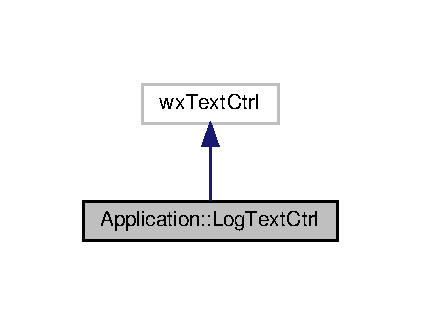
\includegraphics[width=202pt]{class_application_1_1_log_text_ctrl__inherit__graph}
\end{center}
\end{figure}


Collaboration diagram for Application\+:\+:Log\+Text\+Ctrl\+:
\nopagebreak
\begin{figure}[H]
\begin{center}
\leavevmode
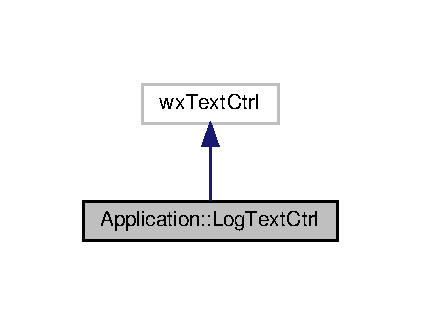
\includegraphics[width=202pt]{class_application_1_1_log_text_ctrl__coll__graph}
\end{center}
\end{figure}
\subsection*{Public Member Functions}
\begin{DoxyCompactItemize}
\item 
virtual void \hyperlink{class_application_1_1_log_text_ctrl_aecf20eb2fc19af8632542de0166a050e}{log} (const std\+::string \&a\+String)
\end{DoxyCompactItemize}
\begin{Indent}{\bf Constructors and destructor}\par
\begin{DoxyCompactItemize}
\item 
{\bfseries Log\+Text\+Ctrl} (Window $\ast$a\+Parent, Window\+Id a\+Window\+Id=D\+E\+F\+A\+U\+L\+T\+\_\+\+ID, long a\+Style=wx\+T\+E\+\_\+\+R\+E\+A\+D\+O\+N\+LY$\vert$wx\+T\+E\+\_\+\+M\+U\+L\+T\+I\+L\+I\+NE$\vert$wx\+T\+E\+\_\+\+D\+O\+N\+T\+W\+R\+AP, const std\+::string \&an\+Initial\+Text=\char`\"{}\char`\"{}, const Point \&a\+Point=Default\+Position, const Size \&a\+Size=Default\+Size)\hypertarget{class_application_1_1_log_text_ctrl_aded0f03a723158ab1a3d2de74a3c8262}{}\label{class_application_1_1_log_text_ctrl_aded0f03a723158ab1a3d2de74a3c8262}

\item 
virtual {\bfseries $\sim$\+Log\+Text\+Ctrl} ()\hypertarget{class_application_1_1_log_text_ctrl_a02828be6cb16c6c772f881757f61c7af}{}\label{class_application_1_1_log_text_ctrl_a02828be6cb16c6c772f881757f61c7af}

\end{DoxyCompactItemize}
\end{Indent}
\subsection*{Protected Member Functions}
\begin{DoxyCompactItemize}
\item 
void \hyperlink{class_application_1_1_log_text_ctrl_af03d3d9049d7a9c13de10d249751fc5e}{On\+Command\+Event} (Command\+Event \&an\+Event)
\end{DoxyCompactItemize}


\subsection{Detailed Description}
A text widget that accepts the tracing of a trace function. 

\subsection{Member Function Documentation}
\index{Application\+::\+Log\+Text\+Ctrl@{Application\+::\+Log\+Text\+Ctrl}!log@{log}}
\index{log@{log}!Application\+::\+Log\+Text\+Ctrl@{Application\+::\+Log\+Text\+Ctrl}}
\subsubsection[{\texorpdfstring{log(const std\+::string \&a\+String)}{log(const std::string &aString)}}]{\setlength{\rightskip}{0pt plus 5cm}void Application\+::\+Log\+Text\+Ctrl\+::log (
\begin{DoxyParamCaption}
\item[{const std\+::string \&}]{a\+String}
\end{DoxyParamCaption}
)\hspace{0.3cm}{\ttfamily [virtual]}}\hypertarget{class_application_1_1_log_text_ctrl_aecf20eb2fc19af8632542de0166a050e}{}\label{class_application_1_1_log_text_ctrl_aecf20eb2fc19af8632542de0166a050e}

\begin{DoxyParams}{Parameters}
{\em a\+String} & \\
\hline
\end{DoxyParams}
\index{Application\+::\+Log\+Text\+Ctrl@{Application\+::\+Log\+Text\+Ctrl}!On\+Command\+Event@{On\+Command\+Event}}
\index{On\+Command\+Event@{On\+Command\+Event}!Application\+::\+Log\+Text\+Ctrl@{Application\+::\+Log\+Text\+Ctrl}}
\subsubsection[{\texorpdfstring{On\+Command\+Event(\+Command\+Event \&an\+Event)}{OnCommandEvent(CommandEvent &anEvent)}}]{\setlength{\rightskip}{0pt plus 5cm}void Application\+::\+Log\+Text\+Ctrl\+::\+On\+Command\+Event (
\begin{DoxyParamCaption}
\item[{Command\+Event \&}]{an\+Event}
\end{DoxyParamCaption}
)\hspace{0.3cm}{\ttfamily [protected]}}\hypertarget{class_application_1_1_log_text_ctrl_af03d3d9049d7a9c13de10d249751fc5e}{}\label{class_application_1_1_log_text_ctrl_af03d3d9049d7a9c13de10d249751fc5e}

\begin{DoxyParams}{Parameters}
{\em an\+Event} & \\
\hline
\end{DoxyParams}


The documentation for this class was generated from the following files\+:\begin{DoxyCompactItemize}
\item 
/home/hqnders/\+Documents/robotworld/src/Log\+Text\+Ctrl.\+hpp\item 
/home/hqnders/\+Documents/robotworld/src/Log\+Text\+Ctrl.\+cpp\end{DoxyCompactItemize}

\hypertarget{class_application_1_1_main_application}{}\section{Application\+:\+:Main\+Application Class Reference}
\label{class_application_1_1_main_application}\index{Application\+::\+Main\+Application@{Application\+::\+Main\+Application}}


Inheritance diagram for Application\+:\+:Main\+Application\+:
\nopagebreak
\begin{figure}[H]
\begin{center}
\leavevmode
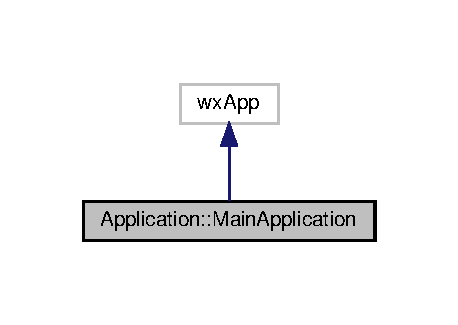
\includegraphics[width=220pt]{class_application_1_1_main_application__inherit__graph}
\end{center}
\end{figure}


Collaboration diagram for Application\+:\+:Main\+Application\+:
\nopagebreak
\begin{figure}[H]
\begin{center}
\leavevmode
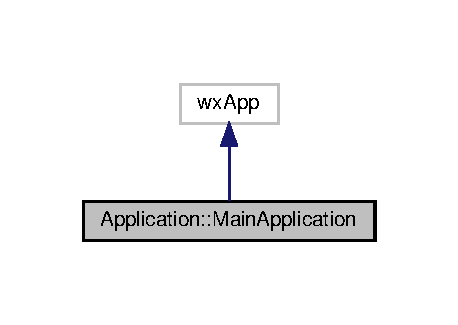
\includegraphics[width=220pt]{class_application_1_1_main_application__coll__graph}
\end{center}
\end{figure}
\subsection*{Public Member Functions}
\begin{DoxyCompactItemize}
\item 
virtual bool \hyperlink{class_application_1_1_main_application_ac9714c4b1debf0d532e2b30224833b53}{On\+Init} ()
\end{DoxyCompactItemize}
\subsection*{Static Public Member Functions}
\begin{Indent}{\bf Command line handling functions}\par
\begin{DoxyCompactItemize}
\item 
static void \hyperlink{class_application_1_1_main_application_abdb7b37eb40ea2884233907a0fc39849}{set\+Commandline\+Arguments} (int argc, char $\ast$argv\mbox{[}$\,$\mbox{]})
\item 
static bool \hyperlink{class_application_1_1_main_application_a973c9c83d80717041866159f1f64609e}{is\+Arg\+Given} (const std\+::string \&a\+Variable)
\item 
static \hyperlink{class_application_1_1_commandline_argument}{Commandline\+Argument} \& \hyperlink{class_application_1_1_main_application_ad696027fcd46221aa7897b8d3e970c83}{get\+Arg} (const std\+::string \&a\+Variable)
\item 
static \hyperlink{class_application_1_1_commandline_argument}{Commandline\+Argument} \& \hyperlink{class_application_1_1_main_application_aac4212439e07c828329b701af43b7c6a}{get\+Arg} (unsigned long an\+Argument\+Number)
\item 
static std\+::vector$<$ std\+::string $>$ \& \hyperlink{class_application_1_1_main_application_a042c7143dd9517896ba9926b43ffeafd}{get\+Commandline\+Files} ()
\end{DoxyCompactItemize}
\end{Indent}


\subsection{Member Function Documentation}
\index{Application\+::\+Main\+Application@{Application\+::\+Main\+Application}!get\+Arg@{get\+Arg}}
\index{get\+Arg@{get\+Arg}!Application\+::\+Main\+Application@{Application\+::\+Main\+Application}}
\subsubsection[{\texorpdfstring{get\+Arg(const std\+::string \&a\+Variable)}{getArg(const std::string &aVariable)}}]{\setlength{\rightskip}{0pt plus 5cm}{\bf Commandline\+Argument} \& Application\+::\+Main\+Application\+::get\+Arg (
\begin{DoxyParamCaption}
\item[{const std\+::string \&}]{a\+Variable}
\end{DoxyParamCaption}
)\hspace{0.3cm}{\ttfamily [static]}}\hypertarget{class_application_1_1_main_application_ad696027fcd46221aa7897b8d3e970c83}{}\label{class_application_1_1_main_application_ad696027fcd46221aa7897b8d3e970c83}

\begin{DoxyParams}{Parameters}
{\em a\+Variable} & The requested variable \\
\hline
\end{DoxyParams}
\begin{DoxyReturn}{Returns}
The requested argument if available, throws an exception otherwise 
\end{DoxyReturn}
\index{Application\+::\+Main\+Application@{Application\+::\+Main\+Application}!get\+Arg@{get\+Arg}}
\index{get\+Arg@{get\+Arg}!Application\+::\+Main\+Application@{Application\+::\+Main\+Application}}
\subsubsection[{\texorpdfstring{get\+Arg(unsigned long an\+Argument\+Number)}{getArg(unsigned long anArgumentNumber)}}]{\setlength{\rightskip}{0pt plus 5cm}{\bf Commandline\+Argument} \& Application\+::\+Main\+Application\+::get\+Arg (
\begin{DoxyParamCaption}
\item[{unsigned long}]{an\+Argument\+Number}
\end{DoxyParamCaption}
)\hspace{0.3cm}{\ttfamily [static]}}\hypertarget{class_application_1_1_main_application_aac4212439e07c828329b701af43b7c6a}{}\label{class_application_1_1_main_application_aac4212439e07c828329b701af43b7c6a}

\begin{DoxyParams}{Parameters}
{\em an\+Argument\+Number} & The requested variable \\
\hline
\end{DoxyParams}
\begin{DoxyReturn}{Returns}
The requested argument if available, throws an exception otherwise 
\end{DoxyReturn}
\index{Application\+::\+Main\+Application@{Application\+::\+Main\+Application}!get\+Commandline\+Files@{get\+Commandline\+Files}}
\index{get\+Commandline\+Files@{get\+Commandline\+Files}!Application\+::\+Main\+Application@{Application\+::\+Main\+Application}}
\subsubsection[{\texorpdfstring{get\+Commandline\+Files()}{getCommandlineFiles()}}]{\setlength{\rightskip}{0pt plus 5cm}std\+::vector$<$ std\+::string $>$ \& Application\+::\+Main\+Application\+::get\+Commandline\+Files (
\begin{DoxyParamCaption}
{}
\end{DoxyParamCaption}
)\hspace{0.3cm}{\ttfamily [static]}}\hypertarget{class_application_1_1_main_application_a042c7143dd9517896ba9926b43ffeafd}{}\label{class_application_1_1_main_application_a042c7143dd9517896ba9926b43ffeafd}
\begin{DoxyReturn}{Returns}
Any files that are given on the command line. 
\end{DoxyReturn}
\index{Application\+::\+Main\+Application@{Application\+::\+Main\+Application}!is\+Arg\+Given@{is\+Arg\+Given}}
\index{is\+Arg\+Given@{is\+Arg\+Given}!Application\+::\+Main\+Application@{Application\+::\+Main\+Application}}
\subsubsection[{\texorpdfstring{is\+Arg\+Given(const std\+::string \&a\+Variable)}{isArgGiven(const std::string &aVariable)}}]{\setlength{\rightskip}{0pt plus 5cm}bool Application\+::\+Main\+Application\+::is\+Arg\+Given (
\begin{DoxyParamCaption}
\item[{const std\+::string \&}]{a\+Variable}
\end{DoxyParamCaption}
)\hspace{0.3cm}{\ttfamily [static]}}\hypertarget{class_application_1_1_main_application_a973c9c83d80717041866159f1f64609e}{}\label{class_application_1_1_main_application_a973c9c83d80717041866159f1f64609e}

\begin{DoxyParams}{Parameters}
{\em a\+Variable} & The format of the variable is implementation defined. Be aware that \char`\"{}-\/\char`\"{} is N\+OT stripped from the argument. The comparisson is done by operator==( const string\&). \\
\hline
\end{DoxyParams}
\begin{DoxyReturn}{Returns}
true if the argument is given, false otherwise. 
\end{DoxyReturn}
\index{Application\+::\+Main\+Application@{Application\+::\+Main\+Application}!On\+Init@{On\+Init}}
\index{On\+Init@{On\+Init}!Application\+::\+Main\+Application@{Application\+::\+Main\+Application}}
\subsubsection[{\texorpdfstring{On\+Init()}{OnInit()}}]{\setlength{\rightskip}{0pt plus 5cm}bool Application\+::\+Main\+Application\+::\+On\+Init (
\begin{DoxyParamCaption}
{}
\end{DoxyParamCaption}
)\hspace{0.3cm}{\ttfamily [virtual]}}\hypertarget{class_application_1_1_main_application_ac9714c4b1debf0d532e2b30224833b53}{}\label{class_application_1_1_main_application_ac9714c4b1debf0d532e2b30224833b53}
This one is called on application startup and is a good place for the app initialisation\+: doing it here and not in the ctor allows to have an error return

\begin{DoxyReturn}{Returns}
If \hyperlink{class_application_1_1_main_application_ac9714c4b1debf0d532e2b30224833b53}{On\+Init()} returns false, the application terminates 
\end{DoxyReturn}
\index{Application\+::\+Main\+Application@{Application\+::\+Main\+Application}!set\+Commandline\+Arguments@{set\+Commandline\+Arguments}}
\index{set\+Commandline\+Arguments@{set\+Commandline\+Arguments}!Application\+::\+Main\+Application@{Application\+::\+Main\+Application}}
\subsubsection[{\texorpdfstring{set\+Commandline\+Arguments(int argc, char $\ast$argv[])}{setCommandlineArguments(int argc, char *argv[])}}]{\setlength{\rightskip}{0pt plus 5cm}void Application\+::\+Main\+Application\+::set\+Commandline\+Arguments (
\begin{DoxyParamCaption}
\item[{int}]{argc, }
\item[{char $\ast$}]{argv\mbox{[}$\,$\mbox{]}}
\end{DoxyParamCaption}
)\hspace{0.3cm}{\ttfamily [static]}}\hypertarget{class_application_1_1_main_application_abdb7b37eb40ea2884233907a0fc39849}{}\label{class_application_1_1_main_application_abdb7b37eb40ea2884233907a0fc39849}
The handling of the arguments is\+:
\begin{DoxyEnumerate}
\item Any argument starting with \char`\"{}-\/\char`\"{} that has \char`\"{}=\char`\"{} in it somewhere is treated as \char`\"{}argument = value\char`\"{}. Spaces are not allowed.
\item Any argument starting with a \char`\"{}-\/\char`\"{} that has no \char`\"{}=\char`\"{} in it somewhere is treated as a boolean with the value \char`\"{}true\char`\"{}. There are no variables that can be false.
\item Arguments without \char`\"{}-\/\char`\"{} prefix are assumed to be files.
\item The \char`\"{}-\/\char`\"{} is N\+OT stripped from the argument.
\end{DoxyEnumerate}


\begin{DoxyParams}{Parameters}
{\em argc} & the count of the arguments \\
\hline
{\em argv} & the array with the values of the arguments \\
\hline
\end{DoxyParams}


The documentation for this class was generated from the following files\+:\begin{DoxyCompactItemize}
\item 
/home/hqnders/\+Documents/robotworld/src/Main\+Application.\+hpp\item 
/home/hqnders/\+Documents/robotworld/src/Main\+Application.\+cpp\end{DoxyCompactItemize}

\hypertarget{class_application_1_1_main_frame_window}{}\section{Application\+:\+:Main\+Frame\+Window Class Reference}
\label{class_application_1_1_main_frame_window}\index{Application\+::\+Main\+Frame\+Window@{Application\+::\+Main\+Frame\+Window}}


Inheritance diagram for Application\+:\+:Main\+Frame\+Window\+:
\nopagebreak
\begin{figure}[H]
\begin{center}
\leavevmode
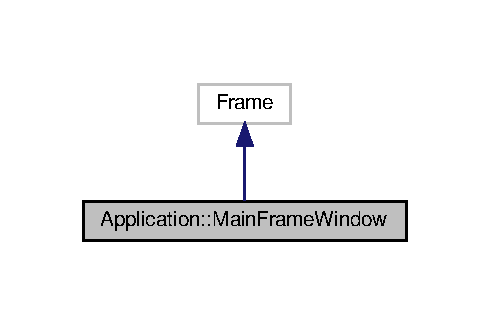
\includegraphics[width=235pt]{class_application_1_1_main_frame_window__inherit__graph}
\end{center}
\end{figure}


Collaboration diagram for Application\+:\+:Main\+Frame\+Window\+:
\nopagebreak
\begin{figure}[H]
\begin{center}
\leavevmode
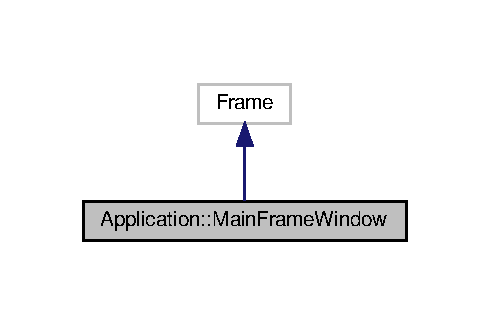
\includegraphics[width=235pt]{class_application_1_1_main_frame_window__coll__graph}
\end{center}
\end{figure}
\subsection*{Public Member Functions}
\begin{DoxyCompactItemize}
\item 
\hyperlink{class_application_1_1_main_frame_window_a6cd8f5a881e4589dc8afa01d5f7ed4ba}{Main\+Frame\+Window} (const std\+::string \&a\+Title)
\item 
\hyperlink{class_base_1_1_debug_trace_function}{Base\+::\+Debug\+Trace\+Function} \& {\bfseries get\+Trace\+Function} () const \hypertarget{class_application_1_1_main_frame_window_a2ab17ead4b86890ec440398eda10273b}{}\label{class_application_1_1_main_frame_window_a2ab17ead4b86890ec440398eda10273b}

\end{DoxyCompactItemize}
\subsection*{Protected Member Functions}
\begin{DoxyCompactItemize}
\item 
void {\bfseries initialise} ()\hypertarget{class_application_1_1_main_frame_window_afbe4226dcd70f22c2ae32062881ceca6}{}\label{class_application_1_1_main_frame_window_afbe4226dcd70f22c2ae32062881ceca6}

\item 
Menu\+Bar $\ast$ {\bfseries initialise\+Menu\+Bar} ()\hypertarget{class_application_1_1_main_frame_window_abdb6890f8b5edd930f93f2fe51a5e181}{}\label{class_application_1_1_main_frame_window_abdb6890f8b5edd930f93f2fe51a5e181}

\item 
Panel $\ast$ {\bfseries initialise\+Client\+Panel} ()\hypertarget{class_application_1_1_main_frame_window_aa9064ca4429720b231234fba743c4b0f}{}\label{class_application_1_1_main_frame_window_aa9064ca4429720b231234fba743c4b0f}

\item 
Splitter\+Window $\ast$ {\bfseries initialise\+Splitter\+Window} ()\hypertarget{class_application_1_1_main_frame_window_a88ea2a7e70bcd1a650c3834883d3deef}{}\label{class_application_1_1_main_frame_window_a88ea2a7e70bcd1a650c3834883d3deef}

\item 
Panel $\ast$ {\bfseries initialise\+Lhs\+Panel} ()\hypertarget{class_application_1_1_main_frame_window_ac0a4ced572ac913cdc441d1a35e97842}{}\label{class_application_1_1_main_frame_window_ac0a4ced572ac913cdc441d1a35e97842}

\item 
Panel $\ast$ {\bfseries initialise\+Rhs\+Panel} ()\hypertarget{class_application_1_1_main_frame_window_a9d9bf15eb75cbce36bca4e22ba144161}{}\label{class_application_1_1_main_frame_window_a9d9bf15eb75cbce36bca4e22ba144161}

\item 
Panel $\ast$ {\bfseries initialise\+Button\+Panel} ()\hypertarget{class_application_1_1_main_frame_window_acc4b68465595b19ab6d23762b7ce1907}{}\label{class_application_1_1_main_frame_window_acc4b68465595b19ab6d23762b7ce1907}

\end{DoxyCompactItemize}


\subsection{Constructor \& Destructor Documentation}
\index{Application\+::\+Main\+Frame\+Window@{Application\+::\+Main\+Frame\+Window}!Main\+Frame\+Window@{Main\+Frame\+Window}}
\index{Main\+Frame\+Window@{Main\+Frame\+Window}!Application\+::\+Main\+Frame\+Window@{Application\+::\+Main\+Frame\+Window}}
\subsubsection[{\texorpdfstring{Main\+Frame\+Window(const std\+::string \&a\+Title)}{MainFrameWindow(const std::string &aTitle)}}]{\setlength{\rightskip}{0pt plus 5cm}Application\+::\+Main\+Frame\+Window\+::\+Main\+Frame\+Window (
\begin{DoxyParamCaption}
\item[{const std\+::string \&}]{a\+Title}
\end{DoxyParamCaption}
)}\hypertarget{class_application_1_1_main_frame_window_a6cd8f5a881e4589dc8afa01d5f7ed4ba}{}\label{class_application_1_1_main_frame_window_a6cd8f5a881e4589dc8afa01d5f7ed4ba}

\begin{DoxyParams}{Parameters}
{\em a\+Title} & The title which is shown in the title bar \\
\hline
\end{DoxyParams}


The documentation for this class was generated from the following files\+:\begin{DoxyCompactItemize}
\item 
/home/hqnders/\+Documents/robotworld/src/Main\+Frame\+Window.\+hpp\item 
/home/hqnders/\+Documents/robotworld/src/Main\+Frame\+Window.\+cpp\end{DoxyCompactItemize}

\hypertarget{class_utils_1_1_math_utils}{}\section{Utils\+:\+:Math\+Utils Class Reference}
\label{class_utils_1_1_math_utils}\index{Utils\+::\+Math\+Utils@{Utils\+::\+Math\+Utils}}
\subsection*{Static Public Member Functions}
\begin{DoxyCompactItemize}
\item 
static float {\bfseries to\+Radians} (float a\+Degrees)\hypertarget{class_utils_1_1_math_utils_a1c1f12a1367c1bb5370e03228f0f7e76}{}\label{class_utils_1_1_math_utils_a1c1f12a1367c1bb5370e03228f0f7e76}

\item 
static float {\bfseries to\+Degrees} (float a\+Radian)\hypertarget{class_utils_1_1_math_utils_a375dca50afb40203156c8e1e30354659}{}\label{class_utils_1_1_math_utils_a375dca50afb40203156c8e1e30354659}

\end{DoxyCompactItemize}


The documentation for this class was generated from the following files\+:\begin{DoxyCompactItemize}
\item 
/home/hqnders/\+Documents/robotworld/src/Math\+Utils.\+hpp\item 
/home/hqnders/\+Documents/robotworld/src/Math\+Utils.\+cpp\end{DoxyCompactItemize}

\hypertarget{struct_messaging_1_1_message}{}\section{Messaging\+:\+:Message Struct Reference}
\label{struct_messaging_1_1_message}\index{Messaging\+::\+Message@{Messaging\+::\+Message}}
\subsection*{Classes}
\begin{DoxyCompactItemize}
\item 
struct \hyperlink{struct_messaging_1_1_message_1_1_message_header}{Message\+Header}
\end{DoxyCompactItemize}
\subsection*{Public Types}
\begin{DoxyCompactItemize}
\item 
typedef std\+::string {\bfseries Message\+Body}\hypertarget{struct_messaging_1_1_message_a6e58a0f71d17a8950334fca1383fd514}{}\label{struct_messaging_1_1_message_a6e58a0f71d17a8950334fca1383fd514}

\end{DoxyCompactItemize}
\subsection*{Public Member Functions}
\begin{DoxyCompactItemize}
\item 
\hyperlink{struct_messaging_1_1_message_ae70b36c0c4ec25e5e622202efaf82513}{Message} (char a\+Message\+Type)
\item 
\hyperlink{struct_messaging_1_1_message_a0771c811ee4035a8fea938b1e79fbfce}{Message} (char a\+Message\+Type, const std\+::string \&a\+Message)
\item 
\hyperlink{struct_messaging_1_1_message_ad8b7c8ca68f83e15e37d8caf28797cbf}{Message} (const \hyperlink{struct_messaging_1_1_message}{Message} \&a\+Message)
\item 
\hyperlink{struct_messaging_1_1_message_1_1_message_header}{Message\+Header} \hyperlink{struct_messaging_1_1_message_abb173c7d9557a5dc08aae8e7b114d87d}{get\+Header} () const 
\item 
void \hyperlink{struct_messaging_1_1_message_aa5d6274a086f01a52853a0536316402e}{set\+Header} (const \hyperlink{struct_messaging_1_1_message_1_1_message_header}{Message\+Header} \&a\+Header)
\item 
char \hyperlink{struct_messaging_1_1_message_af035748b0a1426a8b73f74d85f120be0}{get\+Message\+Type} () const 
\item 
void \hyperlink{struct_messaging_1_1_message_a9a63d50cbf443564d6092d532495f95f}{set\+Message\+Type} (char a\+Message\+Type)
\item 
Message\+Body \hyperlink{struct_messaging_1_1_message_a83ac5ea677d87bc22d56c545bf61127e}{get\+Body} () const 
\item 
void \hyperlink{struct_messaging_1_1_message_abedc9083e15715ad417043e6c483818e}{set\+Body} (const std\+::string \&a\+Body)
\item 
unsigned long \hyperlink{struct_messaging_1_1_message_a61baa8ab016b7b6d07ceade6268db5af}{length} () const 
\end{DoxyCompactItemize}
\begin{Indent}{\bf Debug functions}\par
\begin{DoxyCompactItemize}
\item 
virtual std\+::string \hyperlink{struct_messaging_1_1_message_ac20fb163de9035e2050a04de9ad176d5}{as\+String} () const 
\item 
virtual std\+::string \hyperlink{struct_messaging_1_1_message_a179ec6c4dc374ca0035aa5141522756f}{as\+Debug\+String} () const 
\end{DoxyCompactItemize}
\end{Indent}
\subsection*{Public Attributes}
\begin{DoxyCompactItemize}
\item 
char {\bfseries message\+Type}\hypertarget{struct_messaging_1_1_message_a3a27bf3f32d43a3a9f3980a408ba5061}{}\label{struct_messaging_1_1_message_a3a27bf3f32d43a3a9f3980a408ba5061}

\item 
Message\+Body {\bfseries message}\hypertarget{struct_messaging_1_1_message_ae6af5cd6b85d80ff2769f94be6bf02da}{}\label{struct_messaging_1_1_message_ae6af5cd6b85d80ff2769f94be6bf02da}

\end{DoxyCompactItemize}


\subsection{Constructor \& Destructor Documentation}
\index{Messaging\+::\+Message@{Messaging\+::\+Message}!Message@{Message}}
\index{Message@{Message}!Messaging\+::\+Message@{Messaging\+::\+Message}}
\subsubsection[{\texorpdfstring{Message(char a\+Message\+Type)}{Message(char aMessageType)}}]{\setlength{\rightskip}{0pt plus 5cm}Messaging\+::\+Message\+::\+Message (
\begin{DoxyParamCaption}
\item[{char}]{a\+Message\+Type}
\end{DoxyParamCaption}
)\hspace{0.3cm}{\ttfamily [inline]}}\hypertarget{struct_messaging_1_1_message_ae70b36c0c4ec25e5e622202efaf82513}{}\label{struct_messaging_1_1_message_ae70b36c0c4ec25e5e622202efaf82513}

\begin{DoxyParams}{Parameters}
{\em a\+Message\+Type} & \\
\hline
\end{DoxyParams}
\index{Messaging\+::\+Message@{Messaging\+::\+Message}!Message@{Message}}
\index{Message@{Message}!Messaging\+::\+Message@{Messaging\+::\+Message}}
\subsubsection[{\texorpdfstring{Message(char a\+Message\+Type, const std\+::string \&a\+Message)}{Message(char aMessageType, const std::string &aMessage)}}]{\setlength{\rightskip}{0pt plus 5cm}Messaging\+::\+Message\+::\+Message (
\begin{DoxyParamCaption}
\item[{char}]{a\+Message\+Type, }
\item[{const std\+::string \&}]{a\+Message}
\end{DoxyParamCaption}
)\hspace{0.3cm}{\ttfamily [inline]}}\hypertarget{struct_messaging_1_1_message_a0771c811ee4035a8fea938b1e79fbfce}{}\label{struct_messaging_1_1_message_a0771c811ee4035a8fea938b1e79fbfce}

\begin{DoxyParams}{Parameters}
{\em a\+Message\+Type} & \\
\hline
{\em a\+Message} & \\
\hline
\end{DoxyParams}
\index{Messaging\+::\+Message@{Messaging\+::\+Message}!Message@{Message}}
\index{Message@{Message}!Messaging\+::\+Message@{Messaging\+::\+Message}}
\subsubsection[{\texorpdfstring{Message(const Message \&a\+Message)}{Message(const Message &aMessage)}}]{\setlength{\rightskip}{0pt plus 5cm}Messaging\+::\+Message\+::\+Message (
\begin{DoxyParamCaption}
\item[{const {\bf Message} \&}]{a\+Message}
\end{DoxyParamCaption}
)\hspace{0.3cm}{\ttfamily [inline]}}\hypertarget{struct_messaging_1_1_message_ad8b7c8ca68f83e15e37d8caf28797cbf}{}\label{struct_messaging_1_1_message_ad8b7c8ca68f83e15e37d8caf28797cbf}

\begin{DoxyParams}{Parameters}
{\em a\+Message} & \\
\hline
\end{DoxyParams}


\subsection{Member Function Documentation}
\index{Messaging\+::\+Message@{Messaging\+::\+Message}!as\+Debug\+String@{as\+Debug\+String}}
\index{as\+Debug\+String@{as\+Debug\+String}!Messaging\+::\+Message@{Messaging\+::\+Message}}
\subsubsection[{\texorpdfstring{as\+Debug\+String() const }{asDebugString() const }}]{\setlength{\rightskip}{0pt plus 5cm}virtual std\+::string Messaging\+::\+Message\+::as\+Debug\+String (
\begin{DoxyParamCaption}
{}
\end{DoxyParamCaption}
) const\hspace{0.3cm}{\ttfamily [inline]}, {\ttfamily [virtual]}}\hypertarget{struct_messaging_1_1_message_a179ec6c4dc374ca0035aa5141522756f}{}\label{struct_messaging_1_1_message_a179ec6c4dc374ca0035aa5141522756f}
Returns a description of the object with all data of the object usable for debugging \index{Messaging\+::\+Message@{Messaging\+::\+Message}!as\+String@{as\+String}}
\index{as\+String@{as\+String}!Messaging\+::\+Message@{Messaging\+::\+Message}}
\subsubsection[{\texorpdfstring{as\+String() const }{asString() const }}]{\setlength{\rightskip}{0pt plus 5cm}virtual std\+::string Messaging\+::\+Message\+::as\+String (
\begin{DoxyParamCaption}
{}
\end{DoxyParamCaption}
) const\hspace{0.3cm}{\ttfamily [inline]}, {\ttfamily [virtual]}}\hypertarget{struct_messaging_1_1_message_ac20fb163de9035e2050a04de9ad176d5}{}\label{struct_messaging_1_1_message_ac20fb163de9035e2050a04de9ad176d5}
Returns a 1-\/line description of the object \index{Messaging\+::\+Message@{Messaging\+::\+Message}!get\+Body@{get\+Body}}
\index{get\+Body@{get\+Body}!Messaging\+::\+Message@{Messaging\+::\+Message}}
\subsubsection[{\texorpdfstring{get\+Body() const }{getBody() const }}]{\setlength{\rightskip}{0pt plus 5cm}Message\+Body Messaging\+::\+Message\+::get\+Body (
\begin{DoxyParamCaption}
{}
\end{DoxyParamCaption}
) const\hspace{0.3cm}{\ttfamily [inline]}}\hypertarget{struct_messaging_1_1_message_a83ac5ea677d87bc22d56c545bf61127e}{}\label{struct_messaging_1_1_message_a83ac5ea677d87bc22d56c545bf61127e}
\begin{DoxyReturn}{Returns}

\end{DoxyReturn}
\index{Messaging\+::\+Message@{Messaging\+::\+Message}!get\+Header@{get\+Header}}
\index{get\+Header@{get\+Header}!Messaging\+::\+Message@{Messaging\+::\+Message}}
\subsubsection[{\texorpdfstring{get\+Header() const }{getHeader() const }}]{\setlength{\rightskip}{0pt plus 5cm}{\bf Message\+Header} Messaging\+::\+Message\+::get\+Header (
\begin{DoxyParamCaption}
{}
\end{DoxyParamCaption}
) const\hspace{0.3cm}{\ttfamily [inline]}}\hypertarget{struct_messaging_1_1_message_abb173c7d9557a5dc08aae8e7b114d87d}{}\label{struct_messaging_1_1_message_abb173c7d9557a5dc08aae8e7b114d87d}
\begin{DoxyReturn}{Returns}

\end{DoxyReturn}
\index{Messaging\+::\+Message@{Messaging\+::\+Message}!get\+Message\+Type@{get\+Message\+Type}}
\index{get\+Message\+Type@{get\+Message\+Type}!Messaging\+::\+Message@{Messaging\+::\+Message}}
\subsubsection[{\texorpdfstring{get\+Message\+Type() const }{getMessageType() const }}]{\setlength{\rightskip}{0pt plus 5cm}char Messaging\+::\+Message\+::get\+Message\+Type (
\begin{DoxyParamCaption}
{}
\end{DoxyParamCaption}
) const\hspace{0.3cm}{\ttfamily [inline]}}\hypertarget{struct_messaging_1_1_message_af035748b0a1426a8b73f74d85f120be0}{}\label{struct_messaging_1_1_message_af035748b0a1426a8b73f74d85f120be0}
\begin{DoxyReturn}{Returns}

\end{DoxyReturn}
\index{Messaging\+::\+Message@{Messaging\+::\+Message}!length@{length}}
\index{length@{length}!Messaging\+::\+Message@{Messaging\+::\+Message}}
\subsubsection[{\texorpdfstring{length() const }{length() const }}]{\setlength{\rightskip}{0pt plus 5cm}unsigned long Messaging\+::\+Message\+::length (
\begin{DoxyParamCaption}
{}
\end{DoxyParamCaption}
) const\hspace{0.3cm}{\ttfamily [inline]}}\hypertarget{struct_messaging_1_1_message_a61baa8ab016b7b6d07ceade6268db5af}{}\label{struct_messaging_1_1_message_a61baa8ab016b7b6d07ceade6268db5af}
\begin{DoxyReturn}{Returns}
The length of the message in bytes 
\end{DoxyReturn}
\index{Messaging\+::\+Message@{Messaging\+::\+Message}!set\+Body@{set\+Body}}
\index{set\+Body@{set\+Body}!Messaging\+::\+Message@{Messaging\+::\+Message}}
\subsubsection[{\texorpdfstring{set\+Body(const std\+::string \&a\+Body)}{setBody(const std::string &aBody)}}]{\setlength{\rightskip}{0pt plus 5cm}void Messaging\+::\+Message\+::set\+Body (
\begin{DoxyParamCaption}
\item[{const std\+::string \&}]{a\+Body}
\end{DoxyParamCaption}
)\hspace{0.3cm}{\ttfamily [inline]}}\hypertarget{struct_messaging_1_1_message_abedc9083e15715ad417043e6c483818e}{}\label{struct_messaging_1_1_message_abedc9083e15715ad417043e6c483818e}

\begin{DoxyParams}{Parameters}
{\em a\+Body} & \\
\hline
\end{DoxyParams}
\index{Messaging\+::\+Message@{Messaging\+::\+Message}!set\+Header@{set\+Header}}
\index{set\+Header@{set\+Header}!Messaging\+::\+Message@{Messaging\+::\+Message}}
\subsubsection[{\texorpdfstring{set\+Header(const Message\+Header \&a\+Header)}{setHeader(const MessageHeader &aHeader)}}]{\setlength{\rightskip}{0pt plus 5cm}void Messaging\+::\+Message\+::set\+Header (
\begin{DoxyParamCaption}
\item[{const {\bf Message\+Header} \&}]{a\+Header}
\end{DoxyParamCaption}
)\hspace{0.3cm}{\ttfamily [inline]}}\hypertarget{struct_messaging_1_1_message_aa5d6274a086f01a52853a0536316402e}{}\label{struct_messaging_1_1_message_aa5d6274a086f01a52853a0536316402e}

\begin{DoxyParams}{Parameters}
{\em a\+Header} & \\
\hline
\end{DoxyParams}
\index{Messaging\+::\+Message@{Messaging\+::\+Message}!set\+Message\+Type@{set\+Message\+Type}}
\index{set\+Message\+Type@{set\+Message\+Type}!Messaging\+::\+Message@{Messaging\+::\+Message}}
\subsubsection[{\texorpdfstring{set\+Message\+Type(char a\+Message\+Type)}{setMessageType(char aMessageType)}}]{\setlength{\rightskip}{0pt plus 5cm}void Messaging\+::\+Message\+::set\+Message\+Type (
\begin{DoxyParamCaption}
\item[{char}]{a\+Message\+Type}
\end{DoxyParamCaption}
)\hspace{0.3cm}{\ttfamily [inline]}}\hypertarget{struct_messaging_1_1_message_a9a63d50cbf443564d6092d532495f95f}{}\label{struct_messaging_1_1_message_a9a63d50cbf443564d6092d532495f95f}

\begin{DoxyParams}{Parameters}
{\em a\+Message\+Type} & \\
\hline
\end{DoxyParams}


The documentation for this struct was generated from the following file\+:\begin{DoxyCompactItemize}
\item 
/home/hqnders/\+Documents/robotworld/src/Message.\+hpp\end{DoxyCompactItemize}

\hypertarget{class_messaging_1_1_message_handler}{}\section{Messaging\+:\+:Message\+Handler Class Reference}
\label{class_messaging_1_1_message_handler}\index{Messaging\+::\+Message\+Handler@{Messaging\+::\+Message\+Handler}}


{\ttfamily \#include $<$Message\+Handler.\+hpp$>$}



Inheritance diagram for Messaging\+:\+:Message\+Handler\+:
\nopagebreak
\begin{figure}[H]
\begin{center}
\leavevmode
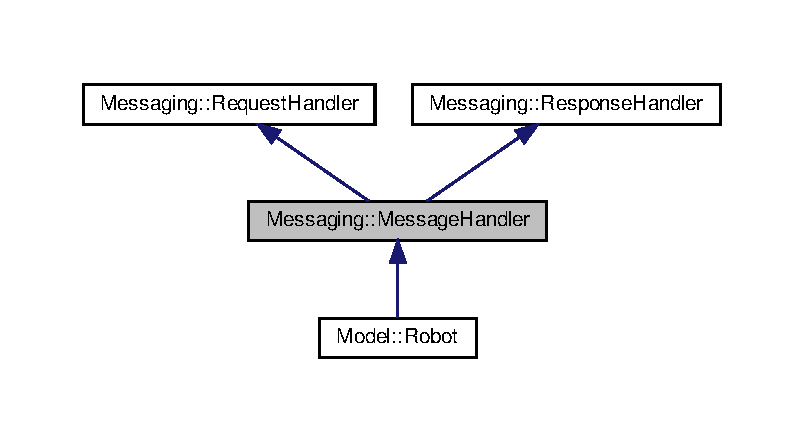
\includegraphics[width=350pt]{class_messaging_1_1_message_handler__inherit__graph}
\end{center}
\end{figure}


Collaboration diagram for Messaging\+:\+:Message\+Handler\+:
\nopagebreak
\begin{figure}[H]
\begin{center}
\leavevmode
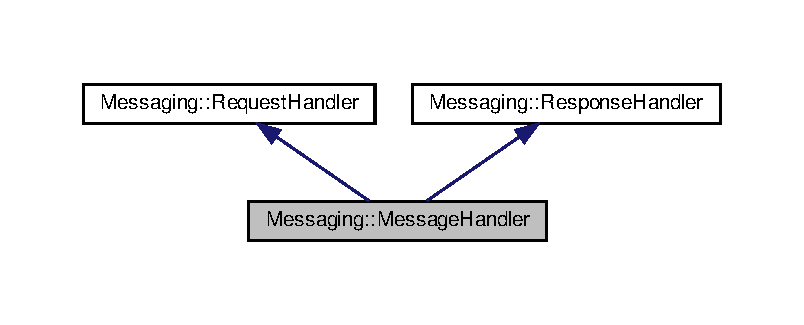
\includegraphics[width=350pt]{class_messaging_1_1_message_handler__coll__graph}
\end{center}
\end{figure}
\subsection*{Additional Inherited Members}


\subsection{Detailed Description}
Convenience interface class for a class that acts both as server and client in the Messaging protocol \begin{DoxySeeAlso}{See also}
\hyperlink{class_messaging_1_1_request_handler_afa23f0ab94ae851a487173a5087da898}{Request\+Handler\+::handle\+Request( Message\& a\+Message)} 

Response\+Handler\+::handle\+Response( Message\& a\+Message) 
\end{DoxySeeAlso}


The documentation for this class was generated from the following file\+:\begin{DoxyCompactItemize}
\item 
/home/hqnders/\+Documents/robotworld/src/Message\+Handler.\+hpp\end{DoxyCompactItemize}

\hypertarget{struct_messaging_1_1_message_1_1_message_header}{}\section{Messaging\+:\+:Message\+:\+:Message\+Header Struct Reference}
\label{struct_messaging_1_1_message_1_1_message_header}\index{Messaging\+::\+Message\+::\+Message\+Header@{Messaging\+::\+Message\+::\+Message\+Header}}
\subsection*{Public Member Functions}
\begin{DoxyCompactItemize}
\item 
\hyperlink{struct_messaging_1_1_message_1_1_message_header_a4c1145a87de865721d59faba878540fe}{Message\+Header} (char a\+Message\+Type, unsigned long a\+Message\+Length)
\item 
\hyperlink{struct_messaging_1_1_message_1_1_message_header_acc197565a5646945320b275fc7432757}{Message\+Header} (const std\+::string \&a\+Message\+Header\+Buffer)
\item 
std\+::string \hyperlink{struct_messaging_1_1_message_1_1_message_header_a116958570c3ee6e61949d3f25c58d0d6}{to\+String} () const 
\item 
void \hyperlink{struct_messaging_1_1_message_1_1_message_header_a2d6cc32d14554859cc042ae608daee6e}{from\+String} (const std\+::string \&a\+String)
\item 
unsigned long \hyperlink{struct_messaging_1_1_message_1_1_message_header_a0d33aa180bd6d8dc9e34b02b4fe3e492}{get\+Header\+Length} () const 
\item 
char \hyperlink{struct_messaging_1_1_message_1_1_message_header_aef4edcff25790eb3120399b96f8c88d1}{get\+Message\+Type} () const 
\item 
unsigned long \hyperlink{struct_messaging_1_1_message_1_1_message_header_aa89056eba883f701deb9a9fe12b27ffa}{get\+Message\+Length} () const 
\end{DoxyCompactItemize}
\begin{Indent}{\bf Debug functions}\par
\begin{DoxyCompactItemize}
\item 
std\+::string \hyperlink{struct_messaging_1_1_message_1_1_message_header_acdae8972e623d75bd1c7f84e9bf88112}{as\+String} () const 
\end{DoxyCompactItemize}
\end{Indent}
\subsection*{Public Attributes}
\begin{DoxyCompactItemize}
\item 
char {\bfseries message\+Type}\hypertarget{struct_messaging_1_1_message_1_1_message_header_a6a51bcb96a297b4c089379b3726689d7}{}\label{struct_messaging_1_1_message_1_1_message_header_a6a51bcb96a297b4c089379b3726689d7}

\item 
unsigned long {\bfseries message\+Length}\hypertarget{struct_messaging_1_1_message_1_1_message_header_a3aeb117ad4e013955cf32cf217ade75a}{}\label{struct_messaging_1_1_message_1_1_message_header_a3aeb117ad4e013955cf32cf217ade75a}

\end{DoxyCompactItemize}
\subsection*{Static Public Attributes}
\begin{DoxyCompactItemize}
\item 
static const char {\bfseries magic\+Number1} = \textquotesingle{}A\textquotesingle{}\hypertarget{struct_messaging_1_1_message_1_1_message_header_ab7d9a533bcbcc875e0c71a854a8d3d7f}{}\label{struct_messaging_1_1_message_1_1_message_header_ab7d9a533bcbcc875e0c71a854a8d3d7f}

\item 
static const char {\bfseries magic\+Number2} = \textquotesingle{}S\textquotesingle{}\hypertarget{struct_messaging_1_1_message_1_1_message_header_abfc4eabe7cc23af31fcf67be7d3f71bd}{}\label{struct_messaging_1_1_message_1_1_message_header_abfc4eabe7cc23af31fcf67be7d3f71bd}

\item 
static const char {\bfseries magic\+Number3} = \textquotesingle{}I\textquotesingle{}\hypertarget{struct_messaging_1_1_message_1_1_message_header_a24692db229162cdaf60b3b7ec52a98f2}{}\label{struct_messaging_1_1_message_1_1_message_header_a24692db229162cdaf60b3b7ec52a98f2}

\item 
static const char {\bfseries magic\+Number4} = \textquotesingle{}O\textquotesingle{}\hypertarget{struct_messaging_1_1_message_1_1_message_header_a59e0cecbb4cb66668d6a75cc57c884c8}{}\label{struct_messaging_1_1_message_1_1_message_header_a59e0cecbb4cb66668d6a75cc57c884c8}

\item 
static const char {\bfseries major\+Version} = \textquotesingle{}1\textquotesingle{}\hypertarget{struct_messaging_1_1_message_1_1_message_header_aa5c450f8bd19792759093880a748c014}{}\label{struct_messaging_1_1_message_1_1_message_header_aa5c450f8bd19792759093880a748c014}

\item 
static const char {\bfseries minor\+Version} = \textquotesingle{}0\textquotesingle{}\hypertarget{struct_messaging_1_1_message_1_1_message_header_ad4d770dcf9125f64181d9373c9a324fd}{}\label{struct_messaging_1_1_message_1_1_message_header_ad4d770dcf9125f64181d9373c9a324fd}

\end{DoxyCompactItemize}


\subsection{Constructor \& Destructor Documentation}
\index{Messaging\+::\+Message\+::\+Message\+Header@{Messaging\+::\+Message\+::\+Message\+Header}!Message\+Header@{Message\+Header}}
\index{Message\+Header@{Message\+Header}!Messaging\+::\+Message\+::\+Message\+Header@{Messaging\+::\+Message\+::\+Message\+Header}}
\subsubsection[{\texorpdfstring{Message\+Header(char a\+Message\+Type, unsigned long a\+Message\+Length)}{MessageHeader(char aMessageType, unsigned long aMessageLength)}}]{\setlength{\rightskip}{0pt plus 5cm}Messaging\+::\+Message\+::\+Message\+Header\+::\+Message\+Header (
\begin{DoxyParamCaption}
\item[{char}]{a\+Message\+Type, }
\item[{unsigned long}]{a\+Message\+Length}
\end{DoxyParamCaption}
)\hspace{0.3cm}{\ttfamily [inline]}}\hypertarget{struct_messaging_1_1_message_1_1_message_header_a4c1145a87de865721d59faba878540fe}{}\label{struct_messaging_1_1_message_1_1_message_header_a4c1145a87de865721d59faba878540fe}

\begin{DoxyParams}{Parameters}
{\em a\+Message\+Type} & \\
\hline
{\em a\+Message\+Length} & \\
\hline
\end{DoxyParams}
\index{Messaging\+::\+Message\+::\+Message\+Header@{Messaging\+::\+Message\+::\+Message\+Header}!Message\+Header@{Message\+Header}}
\index{Message\+Header@{Message\+Header}!Messaging\+::\+Message\+::\+Message\+Header@{Messaging\+::\+Message\+::\+Message\+Header}}
\subsubsection[{\texorpdfstring{Message\+Header(const std\+::string \&a\+Message\+Header\+Buffer)}{MessageHeader(const std::string &aMessageHeaderBuffer)}}]{\setlength{\rightskip}{0pt plus 5cm}Messaging\+::\+Message\+::\+Message\+Header\+::\+Message\+Header (
\begin{DoxyParamCaption}
\item[{const std\+::string \&}]{a\+Message\+Header\+Buffer}
\end{DoxyParamCaption}
)\hspace{0.3cm}{\ttfamily [inline]}}\hypertarget{struct_messaging_1_1_message_1_1_message_header_acc197565a5646945320b275fc7432757}{}\label{struct_messaging_1_1_message_1_1_message_header_acc197565a5646945320b275fc7432757}

\begin{DoxyParams}{Parameters}
{\em a\+Message\+Header\+Buffer} & \\
\hline
\end{DoxyParams}


\subsection{Member Function Documentation}
\index{Messaging\+::\+Message\+::\+Message\+Header@{Messaging\+::\+Message\+::\+Message\+Header}!as\+String@{as\+String}}
\index{as\+String@{as\+String}!Messaging\+::\+Message\+::\+Message\+Header@{Messaging\+::\+Message\+::\+Message\+Header}}
\subsubsection[{\texorpdfstring{as\+String() const }{asString() const }}]{\setlength{\rightskip}{0pt plus 5cm}std\+::string Messaging\+::\+Message\+::\+Message\+Header\+::as\+String (
\begin{DoxyParamCaption}
{}
\end{DoxyParamCaption}
) const\hspace{0.3cm}{\ttfamily [inline]}}\hypertarget{struct_messaging_1_1_message_1_1_message_header_acdae8972e623d75bd1c7f84e9bf88112}{}\label{struct_messaging_1_1_message_1_1_message_header_acdae8972e623d75bd1c7f84e9bf88112}
Returns a 1-\/line description of the object \index{Messaging\+::\+Message\+::\+Message\+Header@{Messaging\+::\+Message\+::\+Message\+Header}!from\+String@{from\+String}}
\index{from\+String@{from\+String}!Messaging\+::\+Message\+::\+Message\+Header@{Messaging\+::\+Message\+::\+Message\+Header}}
\subsubsection[{\texorpdfstring{from\+String(const std\+::string \&a\+String)}{fromString(const std::string &aString)}}]{\setlength{\rightskip}{0pt plus 5cm}void Messaging\+::\+Message\+::\+Message\+Header\+::from\+String (
\begin{DoxyParamCaption}
\item[{const std\+::string \&}]{a\+String}
\end{DoxyParamCaption}
)\hspace{0.3cm}{\ttfamily [inline]}}\hypertarget{struct_messaging_1_1_message_1_1_message_header_a2d6cc32d14554859cc042ae608daee6e}{}\label{struct_messaging_1_1_message_1_1_message_header_a2d6cc32d14554859cc042ae608daee6e}
Stores a A\+S\+C\+II representaion of a message header into this header


\begin{DoxyParams}{Parameters}
{\em a\+String} & \\
\hline
\end{DoxyParams}
\index{Messaging\+::\+Message\+::\+Message\+Header@{Messaging\+::\+Message\+::\+Message\+Header}!get\+Header\+Length@{get\+Header\+Length}}
\index{get\+Header\+Length@{get\+Header\+Length}!Messaging\+::\+Message\+::\+Message\+Header@{Messaging\+::\+Message\+::\+Message\+Header}}
\subsubsection[{\texorpdfstring{get\+Header\+Length() const }{getHeaderLength() const }}]{\setlength{\rightskip}{0pt plus 5cm}unsigned long Messaging\+::\+Message\+::\+Message\+Header\+::get\+Header\+Length (
\begin{DoxyParamCaption}
{}
\end{DoxyParamCaption}
) const\hspace{0.3cm}{\ttfamily [inline]}}\hypertarget{struct_messaging_1_1_message_1_1_message_header_a0d33aa180bd6d8dc9e34b02b4fe3e492}{}\label{struct_messaging_1_1_message_1_1_message_header_a0d33aa180bd6d8dc9e34b02b4fe3e492}
\begin{DoxyReturn}{Returns}
The length of the header in bytes 
\end{DoxyReturn}
\index{Messaging\+::\+Message\+::\+Message\+Header@{Messaging\+::\+Message\+::\+Message\+Header}!get\+Message\+Length@{get\+Message\+Length}}
\index{get\+Message\+Length@{get\+Message\+Length}!Messaging\+::\+Message\+::\+Message\+Header@{Messaging\+::\+Message\+::\+Message\+Header}}
\subsubsection[{\texorpdfstring{get\+Message\+Length() const }{getMessageLength() const }}]{\setlength{\rightskip}{0pt plus 5cm}unsigned long Messaging\+::\+Message\+::\+Message\+Header\+::get\+Message\+Length (
\begin{DoxyParamCaption}
{}
\end{DoxyParamCaption}
) const\hspace{0.3cm}{\ttfamily [inline]}}\hypertarget{struct_messaging_1_1_message_1_1_message_header_aa89056eba883f701deb9a9fe12b27ffa}{}\label{struct_messaging_1_1_message_1_1_message_header_aa89056eba883f701deb9a9fe12b27ffa}
\begin{DoxyReturn}{Returns}
The length of the message in bytes 
\end{DoxyReturn}
\index{Messaging\+::\+Message\+::\+Message\+Header@{Messaging\+::\+Message\+::\+Message\+Header}!get\+Message\+Type@{get\+Message\+Type}}
\index{get\+Message\+Type@{get\+Message\+Type}!Messaging\+::\+Message\+::\+Message\+Header@{Messaging\+::\+Message\+::\+Message\+Header}}
\subsubsection[{\texorpdfstring{get\+Message\+Type() const }{getMessageType() const }}]{\setlength{\rightskip}{0pt plus 5cm}char Messaging\+::\+Message\+::\+Message\+Header\+::get\+Message\+Type (
\begin{DoxyParamCaption}
{}
\end{DoxyParamCaption}
) const\hspace{0.3cm}{\ttfamily [inline]}}\hypertarget{struct_messaging_1_1_message_1_1_message_header_aef4edcff25790eb3120399b96f8c88d1}{}\label{struct_messaging_1_1_message_1_1_message_header_aef4edcff25790eb3120399b96f8c88d1}
\begin{DoxyReturn}{Returns}
The message tpe 
\end{DoxyReturn}
\index{Messaging\+::\+Message\+::\+Message\+Header@{Messaging\+::\+Message\+::\+Message\+Header}!to\+String@{to\+String}}
\index{to\+String@{to\+String}!Messaging\+::\+Message\+::\+Message\+Header@{Messaging\+::\+Message\+::\+Message\+Header}}
\subsubsection[{\texorpdfstring{to\+String() const }{toString() const }}]{\setlength{\rightskip}{0pt plus 5cm}std\+::string Messaging\+::\+Message\+::\+Message\+Header\+::to\+String (
\begin{DoxyParamCaption}
{}
\end{DoxyParamCaption}
) const\hspace{0.3cm}{\ttfamily [inline]}}\hypertarget{struct_messaging_1_1_message_1_1_message_header_a116958570c3ee6e61949d3f25c58d0d6}{}\label{struct_messaging_1_1_message_1_1_message_header_a116958570c3ee6e61949d3f25c58d0d6}
\begin{DoxyReturn}{Returns}
A\+S\+C\+II string representation of the message header 
\end{DoxyReturn}


The documentation for this struct was generated from the following file\+:\begin{DoxyCompactItemize}
\item 
/home/hqnders/\+Documents/robotworld/src/Message.\+hpp\end{DoxyCompactItemize}

\hypertarget{class_model_1_1_model_object}{}\section{model\+:\+:model\+Object Class Reference}
\label{class_model_1_1_model_object}\index{model\+::\+model\+Object@{model\+::\+model\+Object}}


Inheritance diagram for model\+:\+:model\+Object\+:
\nopagebreak
\begin{figure}[H]
\begin{center}
\leavevmode
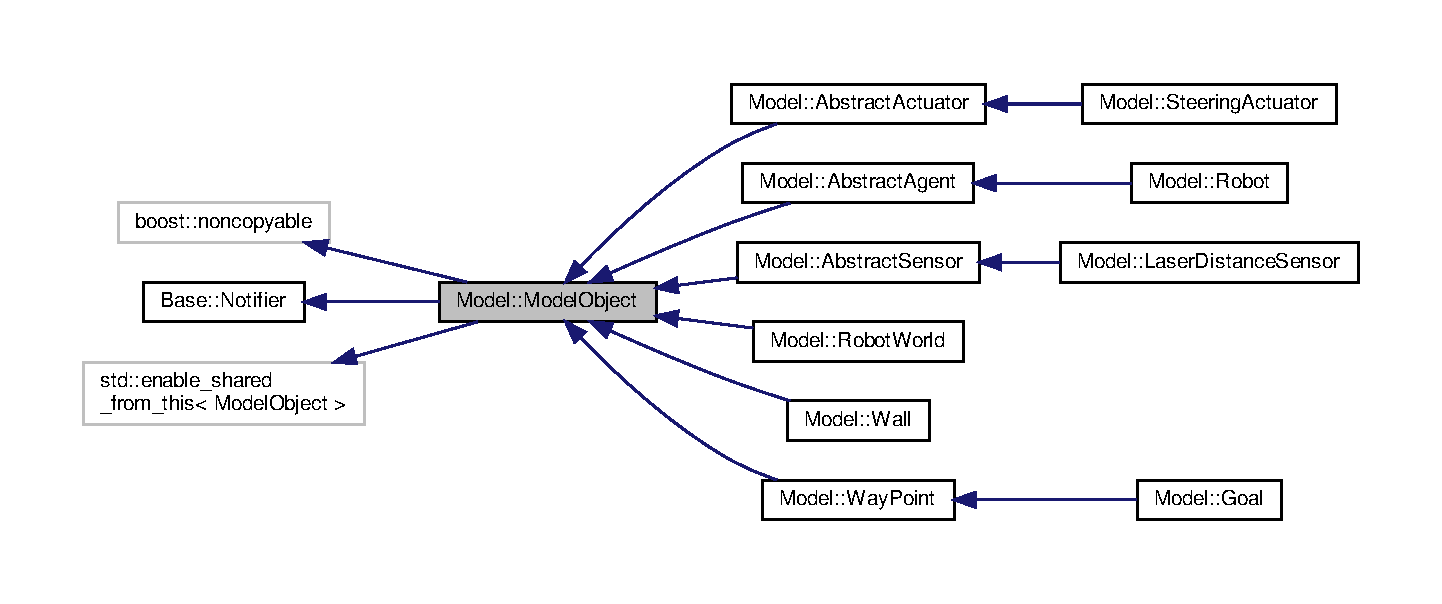
\includegraphics[width=350pt]{class_model_1_1_model_object__inherit__graph}
\end{center}
\end{figure}


Collaboration diagram for model\+:\+:model\+Object\+:
\nopagebreak
\begin{figure}[H]
\begin{center}
\leavevmode
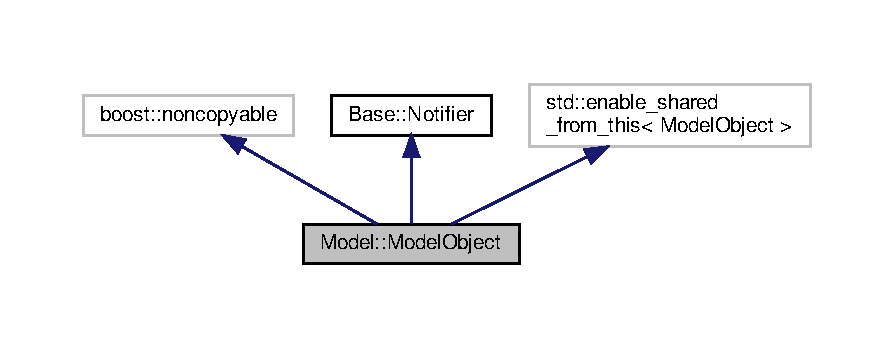
\includegraphics[width=350pt]{class_model_1_1_model_object__coll__graph}
\end{center}
\end{figure}
\subsection*{Public Member Functions}
\begin{DoxyCompactItemize}
\item 
const \hyperlink{class_base_1_1_object_id}{Base\+::\+Object\+Id} \& \hyperlink{class_model_1_1_model_object_afc50aa1e512814a9b6c37a4d3f8b4a97}{get\+Object\+Id} () const 
\item 
{\footnotesize template$<$typename Destination\+Type $>$ }\\std\+::shared\+\_\+ptr$<$ Destination\+Type $>$ \hyperlink{class_model_1_1_model_object_a5330f9a80aeecb0ffe5110fc74258dcb}{to\+Ptr} ()
\end{DoxyCompactItemize}
\begin{Indent}{\bf Constructors and destructor}\par
\begin{DoxyCompactItemize}
\item 
{\bfseries model\+Object} ()\hypertarget{class_model_1_1_model_object_aec6051457cc42ff15ad76dea42278cec}{}\label{class_model_1_1_model_object_aec6051457cc42ff15ad76dea42278cec}

\item 
virtual {\bfseries $\sim$\+model\+Object} ()\hypertarget{class_model_1_1_model_object_a83cf28d0263fca8bbb4003253f767d22}{}\label{class_model_1_1_model_object_a83cf28d0263fca8bbb4003253f767d22}

\end{DoxyCompactItemize}
\end{Indent}
\begin{Indent}{\bf Operators}\par
\begin{DoxyCompactItemize}
\item 
bool \hyperlink{class_model_1_1_model_object_a4dd43ca01fedf5452e9990c1954ada7b}{operator==} (const \hyperlink{class_model_1_1_model_object}{model\+Object} \&a\+model\+Object) const
\item 
bool \hyperlink{class_model_1_1_model_object_a8f5b0be9dabedf96e17cf26dfaa58109}{operator$<$} (const \hyperlink{class_model_1_1_model_object}{model\+Object} \&a\+model\+Object) const
\end{DoxyCompactItemize}
\end{Indent}
\begin{Indent}{\bf Debug functions}\par
\begin{DoxyCompactItemize}
\item 
virtual std\+::string \hyperlink{class_model_1_1_model_object_a9db00b9150a932a1637e425f24c0bdf0}{as\+String} () const 
\item 
virtual std\+::string \hyperlink{class_model_1_1_model_object_aced22b0b0ee637c598c463de6a1d8d03}{as\+Debug\+String} () const 
\end{DoxyCompactItemize}
\end{Indent}


\subsection{Member Function Documentation}
\index{model\+::\+model\+Object@{model\+::\+model\+Object}!as\+Debug\+String@{as\+Debug\+String}}
\index{as\+Debug\+String@{as\+Debug\+String}!model\+::\+model\+Object@{model\+::\+model\+Object}}
\subsubsection[{\texorpdfstring{as\+Debug\+String() const }{asDebugString() const }}]{\setlength{\rightskip}{0pt plus 5cm}std\+::string model\+::\+model\+Object\+::as\+Debug\+String (
\begin{DoxyParamCaption}
{}
\end{DoxyParamCaption}
) const\hspace{0.3cm}{\ttfamily [virtual]}}\hypertarget{class_model_1_1_model_object_aced22b0b0ee637c598c463de6a1d8d03}{}\label{class_model_1_1_model_object_aced22b0b0ee637c598c463de6a1d8d03}
Returns a description of the object with all data of the object usable for debugging 

Reimplemented from \hyperlink{class_base_1_1_notifier_ae9189ab41334252a50dbaa82b6326c12}{Base\+::\+Notifier}.



Reimplemented in \hyperlink{class_model_1_1_robot_aaf05b81b0aff3dac7b39effa462da04e}{model\+::\+Robot}, \hyperlink{class_model_1_1_robot_world_a9c599037d4bdc7ebd4e9138c3cf3cc82}{model\+::\+Robot\+World}, \hyperlink{class_model_1_1_abstract_sensor_aa67bce32b6a602772773f0f23d0634f0}{model\+::\+Abstract\+Sensor}, \hyperlink{class_model_1_1_laser_distance_sensor_ab32d7cbfd19a9a5ec12a0c06ebb02b4f}{model\+::\+Laser\+Distance\+Sensor}, \hyperlink{class_model_1_1_way_point_aa7acf33a786c98fa593a3a38d6270723}{model\+::\+Way\+Point}, \hyperlink{class_model_1_1_abstract_agent_abcb33490b0f5761a2659bf705aff04b5}{model\+::\+Abstract\+Agent}, \hyperlink{class_model_1_1_wall_a298bfdfe9f2d9d637d53b233ec431277}{model\+::\+Wall}, \hyperlink{class_model_1_1_abstract_actuator_ab5199d4458a2913844459832d563f989}{model\+::\+Abstract\+Actuator}, and \hyperlink{class_model_1_1_goal_a30c24f8dfe63a025222753f7d8fa8392}{model\+::\+Goal}.

\index{model\+::\+model\+Object@{model\+::\+model\+Object}!as\+String@{as\+String}}
\index{as\+String@{as\+String}!model\+::\+model\+Object@{model\+::\+model\+Object}}
\subsubsection[{\texorpdfstring{as\+String() const }{asString() const }}]{\setlength{\rightskip}{0pt plus 5cm}std\+::string model\+::\+model\+Object\+::as\+String (
\begin{DoxyParamCaption}
{}
\end{DoxyParamCaption}
) const\hspace{0.3cm}{\ttfamily [virtual]}}\hypertarget{class_model_1_1_model_object_a9db00b9150a932a1637e425f24c0bdf0}{}\label{class_model_1_1_model_object_a9db00b9150a932a1637e425f24c0bdf0}
Returns a 1-\/line description of the object 

Reimplemented from \hyperlink{class_base_1_1_notifier_a5b3d9077ee7023746a05377f2c6b192e}{Base\+::\+Notifier}.



Reimplemented in \hyperlink{class_model_1_1_robot_a888add69a87a3e0f82a3f9c95140716f}{model\+::\+Robot}, \hyperlink{class_model_1_1_robot_world_a9f5a599b9d6523f45df7cbb0aafe4c08}{model\+::\+Robot\+World}, \hyperlink{class_model_1_1_abstract_sensor_a85c18d6d51b8b6a3b97f682ad242be9d}{model\+::\+Abstract\+Sensor}, \hyperlink{class_model_1_1_laser_distance_sensor_a9403593acd21d557e5af1d79901fde34}{model\+::\+Laser\+Distance\+Sensor}, \hyperlink{class_model_1_1_way_point_a2504ccca4e76765faaf91b85c1e0fb75}{model\+::\+Way\+Point}, \hyperlink{class_model_1_1_abstract_agent_a4cee6603af332eb80d524bf3af70489a}{model\+::\+Abstract\+Agent}, \hyperlink{class_model_1_1_wall_af537e51905929a5b583ed5f91e60096b}{model\+::\+Wall}, \hyperlink{class_model_1_1_abstract_actuator_a6fe9d0ac0c7c6c56176fff61a773a4b9}{model\+::\+Abstract\+Actuator}, and \hyperlink{class_model_1_1_goal_a3a2482cbc274b38165125a75be970f29}{model\+::\+Goal}.

\index{model\+::\+model\+Object@{model\+::\+model\+Object}!get\+Object\+Id@{get\+Object\+Id}}
\index{get\+Object\+Id@{get\+Object\+Id}!model\+::\+model\+Object@{model\+::\+model\+Object}}
\subsubsection[{\texorpdfstring{get\+Object\+Id() const }{getObjectId() const }}]{\setlength{\rightskip}{0pt plus 5cm}const {\bf Base\+::\+Object\+Id}\& model\+::\+model\+Object\+::get\+Object\+Id (
\begin{DoxyParamCaption}
{}
\end{DoxyParamCaption}
) const\hspace{0.3cm}{\ttfamily [inline]}}\hypertarget{class_model_1_1_model_object_afc50aa1e512814a9b6c37a4d3f8b4a97}{}\label{class_model_1_1_model_object_afc50aa1e512814a9b6c37a4d3f8b4a97}
\begin{DoxyReturn}{Returns}
the object\+Id (identity) of the \hyperlink{class_model_1_1_model_object}{model\+Object}
\end{DoxyReturn}
\index{model\+::\+model\+Object@{model\+::\+model\+Object}!operator$<$@{operator$<$}}
\index{operator$<$@{operator$<$}!model\+::\+model\+Object@{model\+::\+model\+Object}}
\subsubsection[{\texorpdfstring{operator$<$(const model\+Object \&a\+model\+Object) const }{operator<(const ModelObject &aModelObject) const }}]{\setlength{\rightskip}{0pt plus 5cm}bool model\+::\+model\+Object\+::operator$<$ (
\begin{DoxyParamCaption}
\item[{const {\bf model\+Object} \&}]{a\+model\+Object}
\end{DoxyParamCaption}
) const\hspace{0.3cm}{\ttfamily [inline]}}\hypertarget{class_model_1_1_model_object_a8f5b0be9dabedf96e17cf26dfaa58109}{}\label{class_model_1_1_model_object_a8f5b0be9dabedf96e17cf26dfaa58109}
Less than operator which compares the object\+Ids


\begin{DoxyParams}{Parameters}
{\em a\+model\+Object} & \\
\hline
\end{DoxyParams}
\begin{DoxyReturn}{Returns}
true if lhs.\+object\+Id is less than rhs.\+object\+Id, false otherwise 
\end{DoxyReturn}
\index{model\+::\+model\+Object@{model\+::\+model\+Object}!operator==@{operator==}}
\index{operator==@{operator==}!model\+::\+model\+Object@{model\+::\+model\+Object}}
\subsubsection[{\texorpdfstring{operator==(const model\+Object \&a\+model\+Object) const }{operator==(const ModelObject &aModelObject) const }}]{\setlength{\rightskip}{0pt plus 5cm}bool model\+::\+model\+Object\+::operator== (
\begin{DoxyParamCaption}
\item[{const {\bf model\+Object} \&}]{a\+model\+Object}
\end{DoxyParamCaption}
) const\hspace{0.3cm}{\ttfamily [inline]}}\hypertarget{class_model_1_1_model_object_a4dd43ca01fedf5452e9990c1954ada7b}{}\label{class_model_1_1_model_object_a4dd43ca01fedf5452e9990c1954ada7b}
Equal to operator which compares the object\+Ids


\begin{DoxyParams}{Parameters}
{\em a\+model\+Object} & \\
\hline
\end{DoxyParams}
\begin{DoxyReturn}{Returns}
true if object\+Ids are the same, false otherwise 
\end{DoxyReturn}
\index{model\+::\+model\+Object@{model\+::\+model\+Object}!to\+Ptr@{to\+Ptr}}
\index{to\+Ptr@{to\+Ptr}!model\+::\+model\+Object@{model\+::\+model\+Object}}
\subsubsection[{\texorpdfstring{to\+Ptr()}{toPtr()}}]{\setlength{\rightskip}{0pt plus 5cm}template$<$typename Destination\+Type $>$ std\+::shared\+\_\+ptr$<$Destination\+Type$>$ model\+::\+model\+Object\+::to\+Ptr (
\begin{DoxyParamCaption}
{}
\end{DoxyParamCaption}
)\hspace{0.3cm}{\ttfamily [inline]}}\hypertarget{class_model_1_1_model_object_a5330f9a80aeecb0ffe5110fc74258dcb}{}\label{class_model_1_1_model_object_a5330f9a80aeecb0ffe5110fc74258dcb}
Converts the contained \hyperlink{class_model_1_1_model_object}{model\+Object} to a std\+::shared\+\_\+ptr$<$\+Destination\+Type$>$

\begin{DoxyReturn}{Returns}
std\+::shared\+\_\+ptr$<$\+Destination\+Type$>$ 
\end{DoxyReturn}


The documentation for this class was generated from the following files\+:\begin{DoxyCompactItemize}
\item 
/home/hqnders/\+Documents/robotworld/src/model\+Object.\+hpp\item
/home/hqnders/\+Documents/robotworld/src/model\+Object.\+cpp\end{DoxyCompactItemize}

\hypertarget{struct_base_1_1_notification_function_type_traits}{}\section{Base\+:\+:Notification\+Function\+Type\+Traits$<$ Notification\+Function $>$ Struct Template Reference}
\label{struct_base_1_1_notification_function_type_traits}\index{Base\+::\+Notification\+Function\+Type\+Traits$<$ Notification\+Function $>$@{Base\+::\+Notification\+Function\+Type\+Traits$<$ Notification\+Function $>$}}
\subsection*{Public Member Functions}
\begin{DoxyCompactItemize}
\item 
void {\bfseries call} (Notification\+Function \&a\+Notification\+Function, Notify\+Event \&)\hypertarget{struct_base_1_1_notification_function_type_traits_aec5d2dfeb9d2c47940f7a6e09b81362b}{}\label{struct_base_1_1_notification_function_type_traits_aec5d2dfeb9d2c47940f7a6e09b81362b}

\end{DoxyCompactItemize}


The documentation for this struct was generated from the following file\+:\begin{DoxyCompactItemize}
\item 
/home/hqnders/\+Documents/robotworld/src/Notification\+Function\+Type\+Traits.\+hpp\end{DoxyCompactItemize}

\hypertarget{struct_base_1_1_notification_function_type_traits_3_01std_1_1function_3_01void_07_notify_event_01_6_08_01_4_01_4}{}\section{Base\+:\+:Notification\+Function\+Type\+Traits$<$ std\+:\+:function$<$ void(Notify\+Event \&) $>$ $>$ Struct Template Reference}
\label{struct_base_1_1_notification_function_type_traits_3_01std_1_1function_3_01void_07_notify_event_01_6_08_01_4_01_4}\index{Base\+::\+Notification\+Function\+Type\+Traits$<$ std\+::function$<$ void(\+Notify\+Event \&) $>$ $>$@{Base\+::\+Notification\+Function\+Type\+Traits$<$ std\+::function$<$ void(\+Notify\+Event \&) $>$ $>$}}
\subsection*{Public Member Functions}
\begin{DoxyCompactItemize}
\item 
void {\bfseries call} (std\+::function$<$ void(Notify\+Event \&) $>$ \&a\+Notification\+Function, Notify\+Event \&event)\hypertarget{struct_base_1_1_notification_function_type_traits_3_01std_1_1function_3_01void_07_notify_event_01_6_08_01_4_01_4_a4afd550536d560f3e74fd65452b454d2}{}\label{struct_base_1_1_notification_function_type_traits_3_01std_1_1function_3_01void_07_notify_event_01_6_08_01_4_01_4_a4afd550536d560f3e74fd65452b454d2}

\end{DoxyCompactItemize}


The documentation for this struct was generated from the following file\+:\begin{DoxyCompactItemize}
\item 
/home/hqnders/\+Documents/robotworld/src/Notification\+Function\+Type\+Traits.\+hpp\end{DoxyCompactItemize}

\hypertarget{struct_base_1_1_notification_function_type_traits_tracing}{}\section{Base\+:\+:Notification\+Function\+Type\+Traits\+Tracing Struct Reference}
\label{struct_base_1_1_notification_function_type_traits_tracing}\index{Base\+::\+Notification\+Function\+Type\+Traits\+Tracing@{Base\+::\+Notification\+Function\+Type\+Traits\+Tracing}}


The documentation for this struct was generated from the following file\+:\begin{DoxyCompactItemize}
\item 
/home/hqnders/\+Documents/robotworld/src/Notification\+Function\+Type\+Traits.\+hpp\end{DoxyCompactItemize}

\hypertarget{class_base_1_1_notification_handler}{}\section{Base\+:\+:Notification\+Handler$<$ Notification\+Function $>$ Class Template Reference}
\label{class_base_1_1_notification_handler}\index{Base\+::\+Notification\+Handler$<$ Notification\+Function $>$@{Base\+::\+Notification\+Handler$<$ Notification\+Function $>$}}


Inheritance diagram for Base\+:\+:Notification\+Handler$<$ Notification\+Function $>$\+:
\nopagebreak
\begin{figure}[H]
\begin{center}
\leavevmode
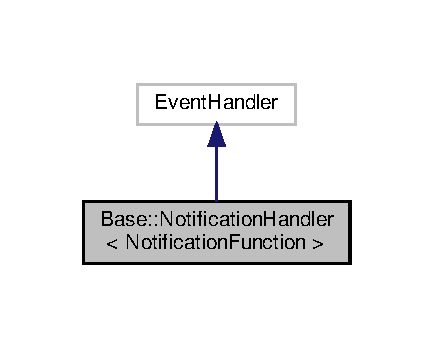
\includegraphics[width=208pt]{class_base_1_1_notification_handler__inherit__graph}
\end{center}
\end{figure}


Collaboration diagram for Base\+:\+:Notification\+Handler$<$ Notification\+Function $>$\+:
\nopagebreak
\begin{figure}[H]
\begin{center}
\leavevmode
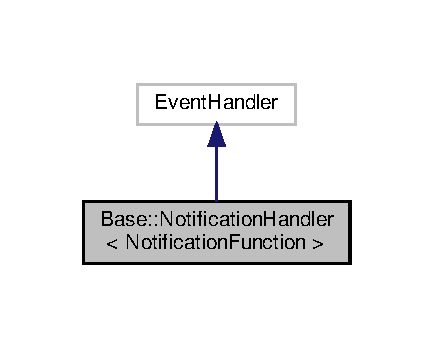
\includegraphics[width=208pt]{class_base_1_1_notification_handler__coll__graph}
\end{center}
\end{figure}
\subsection*{Public Member Functions}
\begin{DoxyCompactItemize}
\item 
{\bfseries Notification\+Handler} (const Notification\+Function \&a\+Notification\+Function)\hypertarget{class_base_1_1_notification_handler_afcd3ef66adda7297131dc6abdef0122e}{}\label{class_base_1_1_notification_handler_afcd3ef66adda7297131dc6abdef0122e}

\item 
void {\bfseries On\+Notification\+Event} (Notify\+Event \&a\+Notify\+Event)\hypertarget{class_base_1_1_notification_handler_a1071e6455f5e96e93f1b6645f7d9bcde}{}\label{class_base_1_1_notification_handler_a1071e6455f5e96e93f1b6645f7d9bcde}

\end{DoxyCompactItemize}


The documentation for this class was generated from the following file\+:\begin{DoxyCompactItemize}
\item 
/home/hqnders/\+Documents/robotworld/src/Notification\+Handler.\+hpp\end{DoxyCompactItemize}

\hypertarget{class_base_1_1_notifier}{}\section{Base\+:\+:Notifier Class Reference}
\label{class_base_1_1_notifier}\index{Base\+::\+Notifier@{Base\+::\+Notifier}}


{\ttfamily \#include $<$Notifier.\+hpp$>$}



Inheritance diagram for Base\+:\+:Notifier\+:
\nopagebreak
\begin{figure}[H]
\begin{center}
\leavevmode
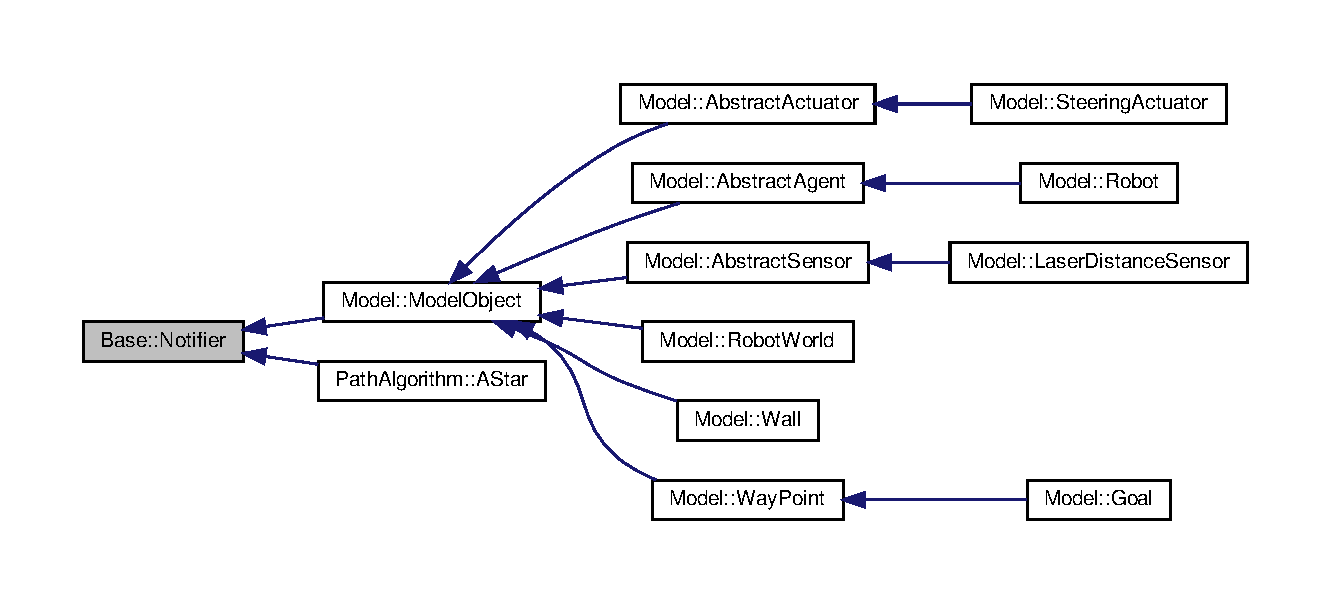
\includegraphics[width=350pt]{class_base_1_1_notifier__inherit__graph}
\end{center}
\end{figure}
\subsection*{Public Member Functions}
\begin{Indent}{\bf Constructors and destructor}\par
\begin{DoxyCompactItemize}
\item 
\hyperlink{class_base_1_1_notifier_ade4bd558bcb722ae11f2dc9b9e0af0a3}{Notifier} (bool enable=true)
\item 
virtual {\bfseries $\sim$\+Notifier} ()\hypertarget{class_base_1_1_notifier_ada72bc1d08008fedeaab951a820717ab}{}\label{class_base_1_1_notifier_ada72bc1d08008fedeaab951a820717ab}

\end{DoxyCompactItemize}
\end{Indent}
\begin{Indent}{\bf Notifier functions}\par
\begin{DoxyCompactItemize}
\item 
virtual void \hyperlink{class_base_1_1_notifier_abed77da5cd65a9a37a3b066aaa02e21d}{enable\+Notification} (bool enable=true)
\item 
virtual void \hyperlink{class_base_1_1_notifier_a050d0bbcf113f31cc16cd3b5229c7576}{disable\+Notification} ()
\item 
virtual bool \hyperlink{class_base_1_1_notifier_a2dfb91da06e2150d8b263b804ff93cac}{is\+Enabled\+For\+Notification} () const 
\item 
virtual void \hyperlink{class_base_1_1_notifier_a5c4e89f48f9688c71ffec225717dd79e}{add\+Observer} (\hyperlink{class_base_1_1_observer}{Observer} \&an\+Observer)
\item 
virtual void \hyperlink{class_base_1_1_notifier_abd13a6f822088d759f4464dbe2e6bb88}{remove\+Observer} (\hyperlink{class_base_1_1_observer}{Observer} \&an\+Observer)
\item 
virtual void \hyperlink{class_base_1_1_notifier_a54d234bcf2531b2a96333f8d3876d485}{remove\+All\+Observers} ()
\item 
virtual void \hyperlink{class_base_1_1_notifier_a9a3df81524d8db68dd64f9a26575c6b4}{notify\+Observers} ()
\end{DoxyCompactItemize}
\end{Indent}
\begin{Indent}{\bf Debug functions}\par
\begin{DoxyCompactItemize}
\item 
virtual std\+::string \hyperlink{class_base_1_1_notifier_a5b3d9077ee7023746a05377f2c6b192e}{as\+String} () const 
\item 
virtual std\+::string \hyperlink{class_base_1_1_notifier_ae9189ab41334252a50dbaa82b6326c12}{as\+Debug\+String} () const 
\end{DoxyCompactItemize}
\end{Indent}


\subsection{Detailed Description}
The \hyperlink{class_base_1_1_notifier}{Notifier} class is part of a straight forward implementation of the Observer/\+Notifier pattern

\begin{DoxySeeAlso}{See also}
\hyperlink{class_base_1_1_observer}{Observer} 
\end{DoxySeeAlso}


\subsection{Constructor \& Destructor Documentation}
\index{Base\+::\+Notifier@{Base\+::\+Notifier}!Notifier@{Notifier}}
\index{Notifier@{Notifier}!Base\+::\+Notifier@{Base\+::\+Notifier}}
\subsubsection[{\texorpdfstring{Notifier(bool enable=true)}{Notifier(bool enable=true)}}]{\setlength{\rightskip}{0pt plus 5cm}Base\+::\+Notifier\+::\+Notifier (
\begin{DoxyParamCaption}
\item[{bool}]{enable = {\ttfamily true}}
\end{DoxyParamCaption}
)}\hypertarget{class_base_1_1_notifier_ade4bd558bcb722ae11f2dc9b9e0af0a3}{}\label{class_base_1_1_notifier_ade4bd558bcb722ae11f2dc9b9e0af0a3}
Default constructor, enables notification by default.


\begin{DoxyParams}{Parameters}
{\em enable} & If true, notification is enabled. \\
\hline
\end{DoxyParams}


\subsection{Member Function Documentation}
\index{Base\+::\+Notifier@{Base\+::\+Notifier}!add\+Observer@{add\+Observer}}
\index{add\+Observer@{add\+Observer}!Base\+::\+Notifier@{Base\+::\+Notifier}}
\subsubsection[{\texorpdfstring{add\+Observer(\+Observer \&an\+Observer)}{addObserver(Observer &anObserver)}}]{\setlength{\rightskip}{0pt plus 5cm}void Base\+::\+Notifier\+::add\+Observer (
\begin{DoxyParamCaption}
\item[{{\bf Observer} \&}]{a\+Observer}
\end{DoxyParamCaption}
)\hspace{0.3cm}{\ttfamily [virtual]}}\hypertarget{class_base_1_1_notifier_a5c4e89f48f9688c71ffec225717dd79e}{}\label{class_base_1_1_notifier_a5c4e89f48f9688c71ffec225717dd79e}
Adds the \hyperlink{class_base_1_1_observer}{Observer} to the list of Observers if not in the list yet


\begin{DoxyParams}{Parameters}
{\em an\+Observer} & The observer to add\\
\hline
\end{DoxyParams}
The implementation of operator== uses pointer comparison! \index{Base\+::\+Notifier@{Base\+::\+Notifier}!as\+Debug\+String@{as\+Debug\+String}}
\index{as\+Debug\+String@{as\+Debug\+String}!Base\+::\+Notifier@{Base\+::\+Notifier}}
\subsubsection[{\texorpdfstring{as\+Debug\+String() const }{asDebugString() const }}]{\setlength{\rightskip}{0pt plus 5cm}std\+::string Base\+::\+Notifier\+::as\+Debug\+String (
\begin{DoxyParamCaption}
{}
\end{DoxyParamCaption}
) const\hspace{0.3cm}{\ttfamily [virtual]}}\hypertarget{class_base_1_1_notifier_ae9189ab41334252a50dbaa82b6326c12}{}\label{class_base_1_1_notifier_ae9189ab41334252a50dbaa82b6326c12}
Returns a description of the object with all data of the object usable for debugging 

Reimplemented in \hyperlink{class_model_1_1_robot_aaf05b81b0aff3dac7b39effa462da04e}{model\+::\+Robot}, \hyperlink{class_model_1_1_robot_world_a9c599037d4bdc7ebd4e9138c3cf3cc82}{model\+::\+Robot\+World}, \hyperlink{class_model_1_1_abstract_sensor_aa67bce32b6a602772773f0f23d0634f0}{model\+::\+Abstract\+Sensor}, \hyperlink{class_model_1_1_model_object_aced22b0b0ee637c598c463de6a1d8d03}{model\+::\+model\+Object}, \hyperlink{class_model_1_1_laser_distance_sensor_ab32d7cbfd19a9a5ec12a0c06ebb02b4f}{model\+::\+Laser\+Distance\+Sensor}, \hyperlink{class_model_1_1_way_point_aa7acf33a786c98fa593a3a38d6270723}{model\+::\+Way\+Point}, \hyperlink{class_model_1_1_abstract_agent_abcb33490b0f5761a2659bf705aff04b5}{model\+::\+Abstract\+Agent}, \hyperlink{class_model_1_1_wall_a298bfdfe9f2d9d637d53b233ec431277}{model\+::\+Wall}, \hyperlink{class_model_1_1_abstract_actuator_ab5199d4458a2913844459832d563f989}{model\+::\+Abstract\+Actuator}, and \hyperlink{class_model_1_1_goal_a30c24f8dfe63a025222753f7d8fa8392}{model\+::\+Goal}.

\index{Base\+::\+Notifier@{Base\+::\+Notifier}!as\+String@{as\+String}}
\index{as\+String@{as\+String}!Base\+::\+Notifier@{Base\+::\+Notifier}}
\subsubsection[{\texorpdfstring{as\+String() const }{asString() const }}]{\setlength{\rightskip}{0pt plus 5cm}std\+::string Base\+::\+Notifier\+::as\+String (
\begin{DoxyParamCaption}
{}
\end{DoxyParamCaption}
) const\hspace{0.3cm}{\ttfamily [virtual]}}\hypertarget{class_base_1_1_notifier_a5b3d9077ee7023746a05377f2c6b192e}{}\label{class_base_1_1_notifier_a5b3d9077ee7023746a05377f2c6b192e}
Returns a 1-\/line description of the object 

Reimplemented in \hyperlink{class_model_1_1_robot_a888add69a87a3e0f82a3f9c95140716f}{model\+::\+Robot}, \hyperlink{class_model_1_1_robot_world_a9f5a599b9d6523f45df7cbb0aafe4c08}{model\+::\+Robot\+World}, \hyperlink{class_model_1_1_abstract_sensor_a85c18d6d51b8b6a3b97f682ad242be9d}{model\+::\+Abstract\+Sensor}, \hyperlink{class_model_1_1_model_object_a9db00b9150a932a1637e425f24c0bdf0}{model\+::\+model\+Object}, \hyperlink{class_model_1_1_laser_distance_sensor_a9403593acd21d557e5af1d79901fde34}{model\+::\+Laser\+Distance\+Sensor}, \hyperlink{class_model_1_1_way_point_a2504ccca4e76765faaf91b85c1e0fb75}{model\+::\+Way\+Point}, \hyperlink{class_model_1_1_abstract_agent_a4cee6603af332eb80d524bf3af70489a}{model\+::\+Abstract\+Agent}, \hyperlink{class_model_1_1_wall_af537e51905929a5b583ed5f91e60096b}{model\+::\+Wall}, \hyperlink{class_model_1_1_abstract_actuator_a6fe9d0ac0c7c6c56176fff61a773a4b9}{model\+::\+Abstract\+Actuator}, and \hyperlink{class_model_1_1_goal_a3a2482cbc274b38165125a75be970f29}{model\+::\+Goal}.

\index{Base\+::\+Notifier@{Base\+::\+Notifier}!disable\+Notification@{disable\+Notification}}
\index{disable\+Notification@{disable\+Notification}!Base\+::\+Notifier@{Base\+::\+Notifier}}
\subsubsection[{\texorpdfstring{disable\+Notification()}{disableNotification()}}]{\setlength{\rightskip}{0pt plus 5cm}void Base\+::\+Notifier\+::disable\+Notification (
\begin{DoxyParamCaption}
{}
\end{DoxyParamCaption}
)\hspace{0.3cm}{\ttfamily [virtual]}}\hypertarget{class_base_1_1_notifier_a050d0bbcf113f31cc16cd3b5229c7576}{}\label{class_base_1_1_notifier_a050d0bbcf113f31cc16cd3b5229c7576}
Disables the notification by this \hyperlink{class_base_1_1_notifier}{Notifier} \index{Base\+::\+Notifier@{Base\+::\+Notifier}!enable\+Notification@{enable\+Notification}}
\index{enable\+Notification@{enable\+Notification}!Base\+::\+Notifier@{Base\+::\+Notifier}}
\subsubsection[{\texorpdfstring{enable\+Notification(bool enable=true)}{enableNotification(bool enable=true)}}]{\setlength{\rightskip}{0pt plus 5cm}void Base\+::\+Notifier\+::enable\+Notification (
\begin{DoxyParamCaption}
\item[{bool}]{enable = {\ttfamily true}}
\end{DoxyParamCaption}
)\hspace{0.3cm}{\ttfamily [virtual]}}\hypertarget{class_base_1_1_notifier_abed77da5cd65a9a37a3b066aaa02e21d}{}\label{class_base_1_1_notifier_abed77da5cd65a9a37a3b066aaa02e21d}
En-\/ or disables the notification by this \hyperlink{class_base_1_1_notifier}{Notifier}


\begin{DoxyParams}{Parameters}
{\em enable} & If true (default) enables the notification for this \hyperlink{class_base_1_1_notifier}{Notifier} \\
\hline
\end{DoxyParams}
\index{Base\+::\+Notifier@{Base\+::\+Notifier}!is\+Enabled\+For\+Notification@{is\+Enabled\+For\+Notification}}
\index{is\+Enabled\+For\+Notification@{is\+Enabled\+For\+Notification}!Base\+::\+Notifier@{Base\+::\+Notifier}}
\subsubsection[{\texorpdfstring{is\+Enabled\+For\+Notification() const }{isEnabledForNotification() const }}]{\setlength{\rightskip}{0pt plus 5cm}bool Base\+::\+Notifier\+::is\+Enabled\+For\+Notification (
\begin{DoxyParamCaption}
{}
\end{DoxyParamCaption}
) const\hspace{0.3cm}{\ttfamily [virtual]}}\hypertarget{class_base_1_1_notifier_a2dfb91da06e2150d8b263b804ff93cac}{}\label{class_base_1_1_notifier_a2dfb91da06e2150d8b263b804ff93cac}
\begin{DoxyReturn}{Returns}
True if notification is enabled for this \hyperlink{class_base_1_1_notifier}{Notifier}, false otherwise 
\end{DoxyReturn}
\index{Base\+::\+Notifier@{Base\+::\+Notifier}!notify\+Observers@{notify\+Observers}}
\index{notify\+Observers@{notify\+Observers}!Base\+::\+Notifier@{Base\+::\+Notifier}}
\subsubsection[{\texorpdfstring{notify\+Observers()}{notifyObservers()}}]{\setlength{\rightskip}{0pt plus 5cm}void Base\+::\+Notifier\+::notify\+Observers (
\begin{DoxyParamCaption}
{}
\end{DoxyParamCaption}
)\hspace{0.3cm}{\ttfamily [virtual]}}\hypertarget{class_base_1_1_notifier_a9a3df81524d8db68dd64f9a26575c6b4}{}\label{class_base_1_1_notifier_a9a3df81524d8db68dd64f9a26575c6b4}
Notifies all observers \index{Base\+::\+Notifier@{Base\+::\+Notifier}!remove\+All\+Observers@{remove\+All\+Observers}}
\index{remove\+All\+Observers@{remove\+All\+Observers}!Base\+::\+Notifier@{Base\+::\+Notifier}}
\subsubsection[{\texorpdfstring{remove\+All\+Observers()}{removeAllObservers()}}]{\setlength{\rightskip}{0pt plus 5cm}void Base\+::\+Notifier\+::remove\+All\+Observers (
\begin{DoxyParamCaption}
{}
\end{DoxyParamCaption}
)\hspace{0.3cm}{\ttfamily [virtual]}}\hypertarget{class_base_1_1_notifier_a54d234bcf2531b2a96333f8d3876d485}{}\label{class_base_1_1_notifier_a54d234bcf2531b2a96333f8d3876d485}
Removes all observer from the list of Observers \index{Base\+::\+Notifier@{Base\+::\+Notifier}!remove\+Observer@{remove\+Observer}}
\index{remove\+Observer@{remove\+Observer}!Base\+::\+Notifier@{Base\+::\+Notifier}}
\subsubsection[{\texorpdfstring{remove\+Observer(\+Observer \&an\+Observer)}{removeObserver(Observer &anObserver)}}]{\setlength{\rightskip}{0pt plus 5cm}void Base\+::\+Notifier\+::remove\+Observer (
\begin{DoxyParamCaption}
\item[{{\bf Observer} \&}]{a\+Observer}
\end{DoxyParamCaption}
)\hspace{0.3cm}{\ttfamily [virtual]}}\hypertarget{class_base_1_1_notifier_abd13a6f822088d759f4464dbe2e6bb88}{}\label{class_base_1_1_notifier_abd13a6f822088d759f4464dbe2e6bb88}
Removes the \hyperlink{class_base_1_1_observer}{Observer} from the list of Observers if in the list


\begin{DoxyParams}{Parameters}
{\em an\+Observer} & The \hyperlink{class_base_1_1_observer}{Observer} to remove\\
\hline
\end{DoxyParams}
The implementation of operator== uses pointer comparison! 

The documentation for this class was generated from the following files\+:\begin{DoxyCompactItemize}
\item 
/home/hqnders/\+Documents/robotworld/src/Notifier.\+hpp\item 
/home/hqnders/\+Documents/robotworld/src/Notifier.\+cpp\end{DoxyCompactItemize}

\hypertarget{class_base_1_1_object_id}{}\section{Base\+:\+:Object\+Id Class Reference}
\label{class_base_1_1_object_id}\index{Base\+::\+Object\+Id@{Base\+::\+Object\+Id}}


{\ttfamily \#include $<$Object\+Id.\+hpp$>$}



Inheritance diagram for Base\+:\+:Object\+Id\+:
\nopagebreak
\begin{figure}[H]
\begin{center}
\leavevmode
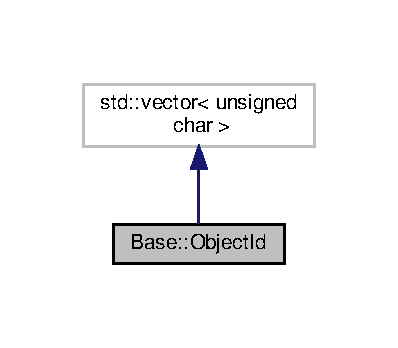
\includegraphics[width=191pt]{class_base_1_1_object_id__inherit__graph}
\end{center}
\end{figure}


Collaboration diagram for Base\+:\+:Object\+Id\+:
\nopagebreak
\begin{figure}[H]
\begin{center}
\leavevmode
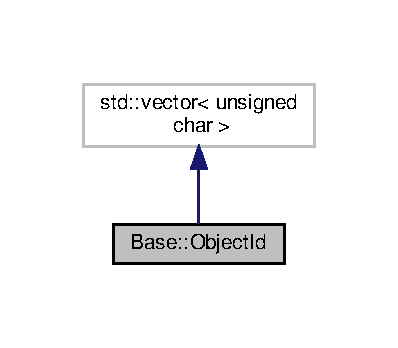
\includegraphics[width=191pt]{class_base_1_1_object_id__coll__graph}
\end{center}
\end{figure}
\subsection*{Public Types}
\begin{DoxyCompactItemize}
\item 
typedef unsigned char {\bfseries value\+\_\+type}\hypertarget{class_base_1_1_object_id_a2a6b8719e9bd362d3cae8a901d238f6f}{}\label{class_base_1_1_object_id_a2a6b8719e9bd362d3cae8a901d238f6f}

\item 
typedef unsigned char $\ast$ {\bfseries pointer}\hypertarget{class_base_1_1_object_id_a36a06bae51c88c5893592b28bd9311e5}{}\label{class_base_1_1_object_id_a36a06bae51c88c5893592b28bd9311e5}

\item 
typedef const unsigned char $\ast$ {\bfseries const\+\_\+pointer}\hypertarget{class_base_1_1_object_id_a1ce45b4d8cec8780cf96e8aa9b921930}{}\label{class_base_1_1_object_id_a1ce45b4d8cec8780cf96e8aa9b921930}

\item 
typedef unsigned char \& {\bfseries reference}\hypertarget{class_base_1_1_object_id_a486ec6587bbbd140dd776281788e98ee}{}\label{class_base_1_1_object_id_a486ec6587bbbd140dd776281788e98ee}

\item 
typedef const unsigned char \& {\bfseries const\+\_\+reference}\hypertarget{class_base_1_1_object_id_a0a971f0617804dc1e107865f3bb473d3}{}\label{class_base_1_1_object_id_a0a971f0617804dc1e107865f3bb473d3}

\item 
typedef std\+::vector$<$ unsigned char $>$ {\bfseries base}\hypertarget{class_base_1_1_object_id_af6e0e53cd168c8de532d458eedefba53}{}\label{class_base_1_1_object_id_af6e0e53cd168c8de532d458eedefba53}

\end{DoxyCompactItemize}
\subsection*{Public Member Functions}
\begin{DoxyCompactItemize}
\item 
{\footnotesize template$<$typename Input\+Iterator $>$ }\\{\bfseries Object\+Id} (Input\+Iterator first, Input\+Iterator last)\hypertarget{class_base_1_1_object_id_a96f9abac9baddbf62eaad80bd1499e72}{}\label{class_base_1_1_object_id_a96f9abac9baddbf62eaad80bd1499e72}

\item 
{\bfseries Object\+Id} (const std\+::string \&an\+Object\+Id\+String)\hypertarget{class_base_1_1_object_id_aca3e55b04c30d9f939f04b2de5aa25c5}{}\label{class_base_1_1_object_id_aca3e55b04c30d9f939f04b2de5aa25c5}

\item 
\hyperlink{class_base_1_1_object_id}{Object\+Id} \& {\bfseries operator=} (const \hyperlink{class_base_1_1_object_id}{Object\+Id} \&an\+Object\+Id)\hypertarget{class_base_1_1_object_id_a449f58cf08f6684639023708b882a00e}{}\label{class_base_1_1_object_id_a449f58cf08f6684639023708b882a00e}

\item 
bool \hyperlink{class_base_1_1_object_id_abe7eb5f3190496d40e1f364b6145e4b2}{operator==} (const \hyperlink{class_base_1_1_object_id}{Object\+Id} \&an\+Object\+Id) const 
\item 
bool \hyperlink{class_base_1_1_object_id_ad69ac55dac3aafd3ea38281ae7d762c0}{operator$<$} (const \hyperlink{class_base_1_1_object_id}{Object\+Id} \&an\+Object\+Id) const 
\item 
std\+::string \hyperlink{class_base_1_1_object_id_af3e9b3d04e1628fa6c1973920fabcd14}{to\+String} () const 
\item 
void \hyperlink{class_base_1_1_object_id_ae32c9ac9ee69665fed2771854da880b6}{from\+String} (const std\+::string \&an\+Object\+Id\+String)
\item 
bool {\bfseries is\+Null} () const \hypertarget{class_base_1_1_object_id_a113567944442dcaebfbb8abe2e8952fb}{}\label{class_base_1_1_object_id_a113567944442dcaebfbb8abe2e8952fb}

\item 
bool {\bfseries is\+Valid} () const \hypertarget{class_base_1_1_object_id_a7b5254288f7bf70ed7a6268abc3b930b}{}\label{class_base_1_1_object_id_a7b5254288f7bf70ed7a6268abc3b930b}

\end{DoxyCompactItemize}
\begin{Indent}{\bf Debug functions}\par
\begin{DoxyCompactItemize}
\item 
std\+::string \hyperlink{class_base_1_1_object_id_afdc5a733d73342473fec933503e49a6e}{as\+String} () const 
\item 
std\+::string \hyperlink{class_base_1_1_object_id_a38e6fd78d084461a0535bd86b998db56}{as\+Debug\+String} () const 
\end{DoxyCompactItemize}
\end{Indent}
\subsection*{Static Public Member Functions}
\begin{DoxyCompactItemize}
\item 
static \hyperlink{class_base_1_1_object_id}{Object\+Id} \hyperlink{class_base_1_1_object_id_a5ec6e05d2302d16274d66c815e43baf9}{new\+Object\+Id} ()
\end{DoxyCompactItemize}
\subsection*{Static Public Attributes}
\begin{DoxyCompactItemize}
\item 
static std\+::string \hyperlink{class_base_1_1_object_id_a8ccba80236842b454cf6e7dda04e12f5}{object\+Id\+Namespace} = \char`\"{}\char`\"{}
\end{DoxyCompactItemize}
\subsection*{C\+O\+R\+BA required interface for Portable\+Server\+:\+:Object\+Id and sequence$<$ T $>$}
\begin{DoxyCompactItemize}
\item 
static pointer \hyperlink{class_base_1_1_object_id_a3028106d58f6db9df06c2faf797f30f8}{allocbuf} (unsigned long nelems)
\item 
static void \hyperlink{class_base_1_1_object_id_a2a50ef3cccf4fd20fd17f2c52fd00c9d}{freebuf} (pointer aT)
\item 
\hyperlink{class_base_1_1_object_id_a62a23904516e14dbef8fee4e5804fa6c}{Object\+Id} ()
\item 
\hyperlink{class_base_1_1_object_id_a198bf2ac34a1ab0150a43c97d8002cec}{Object\+Id} (unsigned long max)
\item 
\hyperlink{class_base_1_1_object_id_a4f0abd7ada085282e495d1a5fab3ea43}{Object\+Id} (unsigned long, unsigned long len, unsigned char $\ast$a\+Data\+Pointer, bool)
\item 
\hyperlink{class_base_1_1_object_id_abdd4924553c835229354677dad7c3c26}{Object\+Id} (const \hyperlink{class_base_1_1_object_id}{Object\+Id} \&an\+Object\+Id)
\item 
virtual \hyperlink{class_base_1_1_object_id_a62fd29d91e79c3c9130f45cbb32275fc}{$\sim$\+Object\+Id} ()
\item 
unsigned long \hyperlink{class_base_1_1_object_id_a4a48d8c6f85bd9fd2991710635d316d8}{maximum} () const 
\item 
void \hyperlink{class_base_1_1_object_id_a2eae06c2581239d292ea3467c3cfdfba}{length} (unsigned long len)
\item 
unsigned long \hyperlink{class_base_1_1_object_id_aad6bf09824bc18612fa6654cb5f0bb0f}{length} () const 
\item 
reference \hyperlink{class_base_1_1_object_id_a518d985d2a670fdcb6ef360e2655e44b}{operator\mbox{[}$\,$\mbox{]}} (unsigned long index)
\item 
const\+\_\+reference \hyperlink{class_base_1_1_object_id_a8a1c7b67bea028bf2073f81751fc3f94}{operator\mbox{[}$\,$\mbox{]}} (unsigned long index) const 
\item 
bool \hyperlink{class_base_1_1_object_id_a27eb724a90e960cdf691c76391cc786d}{release} () const 
\item 
void \hyperlink{class_base_1_1_object_id_a5469cb64007c5007be8ab2893fb3848a}{replace} (unsigned long, unsigned long len, pointer new\+Data, bool)
\item 
pointer \hyperlink{class_base_1_1_object_id_aa91cd5a6d4b78734f903138614098868}{get\+\_\+buffer} (bool orphan=false)
\item 
const\+\_\+pointer \hyperlink{class_base_1_1_object_id_a0f4d8c05f11d882598daf15c2c1cd714}{get\+\_\+buffer} () const 
\end{DoxyCompactItemize}


\subsection{Detailed Description}
The \hyperlink{class_base_1_1_object_id}{Object\+Id} class is also used in Dagda. Therefore it has the required Portable\+Server\+::\+Object\+Id / unbounded sequence interface.

The O\+ID class is 16 bytes, this class is 24 bytes. If one is memory constraint the O\+ID class may be of some help. Be warned\+: the O\+ID class is not actively maintained anymore (but than, who reeds this besides me, the maintainer). 

\subsection{Constructor \& Destructor Documentation}
\index{Base\+::\+Object\+Id@{Base\+::\+Object\+Id}!Object\+Id@{Object\+Id}}
\index{Object\+Id@{Object\+Id}!Base\+::\+Object\+Id@{Base\+::\+Object\+Id}}
\subsubsection[{\texorpdfstring{Object\+Id()}{ObjectId()}}]{\setlength{\rightskip}{0pt plus 5cm}Base\+::\+Object\+Id\+::\+Object\+Id (
\begin{DoxyParamCaption}
{}
\end{DoxyParamCaption}
)\hspace{0.3cm}{\ttfamily [inline]}}\hypertarget{class_base_1_1_object_id_a62a23904516e14dbef8fee4e5804fa6c}{}\label{class_base_1_1_object_id_a62a23904516e14dbef8fee4e5804fa6c}
Default ctor.

Also specified by \index{Base\+::\+Object\+Id@{Base\+::\+Object\+Id}!Object\+Id@{Object\+Id}}
\index{Object\+Id@{Object\+Id}!Base\+::\+Object\+Id@{Base\+::\+Object\+Id}}
\subsubsection[{\texorpdfstring{Object\+Id(unsigned long max)}{ObjectId(unsigned long max)}}]{\setlength{\rightskip}{0pt plus 5cm}Base\+::\+Object\+Id\+::\+Object\+Id (
\begin{DoxyParamCaption}
\item[{unsigned long}]{max}
\end{DoxyParamCaption}
)\hspace{0.3cm}{\ttfamily [inline]}}\hypertarget{class_base_1_1_object_id_a198bf2ac34a1ab0150a43c97d8002cec}{}\label{class_base_1_1_object_id_a198bf2ac34a1ab0150a43c97d8002cec}
Maximum ctor.


\begin{DoxyParams}{Parameters}
{\em max} & Initial elements reservation \\
\hline
\end{DoxyParams}
\index{Base\+::\+Object\+Id@{Base\+::\+Object\+Id}!Object\+Id@{Object\+Id}}
\index{Object\+Id@{Object\+Id}!Base\+::\+Object\+Id@{Base\+::\+Object\+Id}}
\subsubsection[{\texorpdfstring{Object\+Id(unsigned long, unsigned long len, unsigned char $\ast$a\+Data\+Pointer, bool)}{ObjectId(unsigned long, unsigned long len, unsigned char *aDataPointer, bool)}}]{\setlength{\rightskip}{0pt plus 5cm}Base\+::\+Object\+Id\+::\+Object\+Id (
\begin{DoxyParamCaption}
\item[{unsigned}]{long, }
\item[{unsigned long}]{len, }
\item[{unsigned char $\ast$}]{a\+Data\+Pointer, }
\item[{bool}]{}
\end{DoxyParamCaption}
)\hspace{0.3cm}{\ttfamily [inline]}}\hypertarget{class_base_1_1_object_id_a4f0abd7ada085282e495d1a5fab3ea43}{}\label{class_base_1_1_object_id_a4f0abd7ada085282e495d1a5fab3ea43}
Data ctor.


\begin{DoxyParams}{Parameters}
{\em max} & Initial elements reservation. Is actually ignored \\
\hline
{\em length} & Length of the data \\
\hline
{\em data} & Start of the data \\
\hline
{\em release} & If true the sequences owns and manages any containing pointers Is actually ignored and always true. \\
\hline
\end{DoxyParams}
\index{Base\+::\+Object\+Id@{Base\+::\+Object\+Id}!Object\+Id@{Object\+Id}}
\index{Object\+Id@{Object\+Id}!Base\+::\+Object\+Id@{Base\+::\+Object\+Id}}
\subsubsection[{\texorpdfstring{Object\+Id(const Object\+Id \&an\+Object\+Id)}{ObjectId(const ObjectId &anObjectId)}}]{\setlength{\rightskip}{0pt plus 5cm}Base\+::\+Object\+Id\+::\+Object\+Id (
\begin{DoxyParamCaption}
\item[{const {\bf Object\+Id} \&}]{an\+Object\+Id}
\end{DoxyParamCaption}
)\hspace{0.3cm}{\ttfamily [inline]}}\hypertarget{class_base_1_1_object_id_abdd4924553c835229354677dad7c3c26}{}\label{class_base_1_1_object_id_abdd4924553c835229354677dad7c3c26}
Makes a deep copy. \index{Base\+::\+Object\+Id@{Base\+::\+Object\+Id}!````~Object\+Id@{$\sim$\+Object\+Id}}
\index{````~Object\+Id@{$\sim$\+Object\+Id}!Base\+::\+Object\+Id@{Base\+::\+Object\+Id}}
\subsubsection[{\texorpdfstring{$\sim$\+Object\+Id()}{~ObjectId()}}]{\setlength{\rightskip}{0pt plus 5cm}Base\+::\+Object\+Id\+::$\sim$\+Object\+Id (
\begin{DoxyParamCaption}
{}
\end{DoxyParamCaption}
)\hspace{0.3cm}{\ttfamily [virtual]}}\hypertarget{class_base_1_1_object_id_a62fd29d91e79c3c9130f45cbb32275fc}{}\label{class_base_1_1_object_id_a62fd29d91e79c3c9130f45cbb32275fc}
Also specified by Portable\+Server\+::\+Object\+Id and sequence$<$ T $>$ 

\subsection{Member Function Documentation}
\index{Base\+::\+Object\+Id@{Base\+::\+Object\+Id}!allocbuf@{allocbuf}}
\index{allocbuf@{allocbuf}!Base\+::\+Object\+Id@{Base\+::\+Object\+Id}}
\subsubsection[{\texorpdfstring{allocbuf(unsigned long nelems)}{allocbuf(unsigned long nelems)}}]{\setlength{\rightskip}{0pt plus 5cm}static pointer Base\+::\+Object\+Id\+::allocbuf (
\begin{DoxyParamCaption}
\item[{unsigned long}]{nelems}
\end{DoxyParamCaption}
)\hspace{0.3cm}{\ttfamily [inline]}, {\ttfamily [static]}}\hypertarget{class_base_1_1_object_id_a3028106d58f6db9df06c2faf797f30f8}{}\label{class_base_1_1_object_id_a3028106d58f6db9df06c2faf797f30f8}
Do not use. It always throws an Danu\+::\+Invalid\+Request exception.


\begin{DoxyParams}{Parameters}
{\em nelems} & \\
\hline
\end{DoxyParams}
\begin{DoxyReturn}{Returns}
a new-\/ed buffer 
\end{DoxyReturn}
\index{Base\+::\+Object\+Id@{Base\+::\+Object\+Id}!as\+Debug\+String@{as\+Debug\+String}}
\index{as\+Debug\+String@{as\+Debug\+String}!Base\+::\+Object\+Id@{Base\+::\+Object\+Id}}
\subsubsection[{\texorpdfstring{as\+Debug\+String() const }{asDebugString() const }}]{\setlength{\rightskip}{0pt plus 5cm}std\+::string Base\+::\+Object\+Id\+::as\+Debug\+String (
\begin{DoxyParamCaption}
{}
\end{DoxyParamCaption}
) const}\hypertarget{class_base_1_1_object_id_a38e6fd78d084461a0535bd86b998db56}{}\label{class_base_1_1_object_id_a38e6fd78d084461a0535bd86b998db56}
Returns a description of the object with all data of the object usable for debugging \index{Base\+::\+Object\+Id@{Base\+::\+Object\+Id}!as\+String@{as\+String}}
\index{as\+String@{as\+String}!Base\+::\+Object\+Id@{Base\+::\+Object\+Id}}
\subsubsection[{\texorpdfstring{as\+String() const }{asString() const }}]{\setlength{\rightskip}{0pt plus 5cm}std\+::string Base\+::\+Object\+Id\+::as\+String (
\begin{DoxyParamCaption}
{}
\end{DoxyParamCaption}
) const}\hypertarget{class_base_1_1_object_id_afdc5a733d73342473fec933503e49a6e}{}\label{class_base_1_1_object_id_afdc5a733d73342473fec933503e49a6e}
Returns a 1-\/line description of the object \index{Base\+::\+Object\+Id@{Base\+::\+Object\+Id}!freebuf@{freebuf}}
\index{freebuf@{freebuf}!Base\+::\+Object\+Id@{Base\+::\+Object\+Id}}
\subsubsection[{\texorpdfstring{freebuf(pointer a\+T)}{freebuf(pointer aT)}}]{\setlength{\rightskip}{0pt plus 5cm}static void Base\+::\+Object\+Id\+::freebuf (
\begin{DoxyParamCaption}
\item[{pointer}]{aT}
\end{DoxyParamCaption}
)\hspace{0.3cm}{\ttfamily [inline]}, {\ttfamily [static]}}\hypertarget{class_base_1_1_object_id_a2a50ef3cccf4fd20fd17f2c52fd00c9d}{}\label{class_base_1_1_object_id_a2a50ef3cccf4fd20fd17f2c52fd00c9d}
Do not use. It always throws an Danu\+::\+Invalid\+Request exception.


\begin{DoxyParams}{Parameters}
{\em aT} & The buffer to free \\
\hline
\end{DoxyParams}
\index{Base\+::\+Object\+Id@{Base\+::\+Object\+Id}!from\+String@{from\+String}}
\index{from\+String@{from\+String}!Base\+::\+Object\+Id@{Base\+::\+Object\+Id}}
\subsubsection[{\texorpdfstring{from\+String(const std\+::string \&an\+Object\+Id\+String)}{fromString(const std::string &anObjectIdString)}}]{\setlength{\rightskip}{0pt plus 5cm}void Base\+::\+Object\+Id\+::from\+String (
\begin{DoxyParamCaption}
\item[{const std\+::string \&}]{an\+Object\+Id\+String}
\end{DoxyParamCaption}
)\hspace{0.3cm}{\ttfamily [inline]}}\hypertarget{class_base_1_1_object_id_ae32c9ac9ee69665fed2771854da880b6}{}\label{class_base_1_1_object_id_ae32c9ac9ee69665fed2771854da880b6}
Calling obj1.\+from\+String( obj2.\+to\+String()) has the same effect as assignment, obj1 = obj2.


\begin{DoxyParams}{Parameters}
{\em an\+Object\+Id\+String} & A string representation of an \hyperlink{class_base_1_1_object_id}{Object\+Id}. \\
\hline
\end{DoxyParams}
\index{Base\+::\+Object\+Id@{Base\+::\+Object\+Id}!get\+\_\+buffer@{get\+\_\+buffer}}
\index{get\+\_\+buffer@{get\+\_\+buffer}!Base\+::\+Object\+Id@{Base\+::\+Object\+Id}}
\subsubsection[{\texorpdfstring{get\+\_\+buffer(bool orphan=false)}{get_buffer(bool orphan=false)}}]{\setlength{\rightskip}{0pt plus 5cm}pointer Base\+::\+Object\+Id\+::get\+\_\+buffer (
\begin{DoxyParamCaption}
\item[{bool}]{orphan = {\ttfamily false}}
\end{DoxyParamCaption}
)\hspace{0.3cm}{\ttfamily [inline]}}\hypertarget{class_base_1_1_object_id_aa91cd5a6d4b78734f903138614098868}{}\label{class_base_1_1_object_id_aa91cd5a6d4b78734f903138614098868}

\begin{DoxyParams}{Parameters}
{\em orphan} & \\
\hline
\end{DoxyParams}
\begin{DoxyReturn}{Returns}
The \hyperlink{class_base_1_1_object_id}{Object\+Id} as a modifyable continues buffer. If the buffer is modified as that it expands the buffer this  lead to failure eventually 
\end{DoxyReturn}
\index{Base\+::\+Object\+Id@{Base\+::\+Object\+Id}!get\+\_\+buffer@{get\+\_\+buffer}}
\index{get\+\_\+buffer@{get\+\_\+buffer}!Base\+::\+Object\+Id@{Base\+::\+Object\+Id}}
\subsubsection[{\texorpdfstring{get\+\_\+buffer() const }{get_buffer() const }}]{\setlength{\rightskip}{0pt plus 5cm}const\+\_\+pointer Base\+::\+Object\+Id\+::get\+\_\+buffer (
\begin{DoxyParamCaption}
{}
\end{DoxyParamCaption}
) const\hspace{0.3cm}{\ttfamily [inline]}}\hypertarget{class_base_1_1_object_id_a0f4d8c05f11d882598daf15c2c1cd714}{}\label{class_base_1_1_object_id_a0f4d8c05f11d882598daf15c2c1cd714}
\begin{DoxyReturn}{Returns}
The \hyperlink{class_base_1_1_object_id}{Object\+Id} as a readonly continues buffer. 
\end{DoxyReturn}
\index{Base\+::\+Object\+Id@{Base\+::\+Object\+Id}!length@{length}}
\index{length@{length}!Base\+::\+Object\+Id@{Base\+::\+Object\+Id}}
\subsubsection[{\texorpdfstring{length(unsigned long len)}{length(unsigned long len)}}]{\setlength{\rightskip}{0pt plus 5cm}void Base\+::\+Object\+Id\+::length (
\begin{DoxyParamCaption}
\item[{unsigned long}]{len}
\end{DoxyParamCaption}
)\hspace{0.3cm}{\ttfamily [inline]}}\hypertarget{class_base_1_1_object_id_a2eae06c2581239d292ea3467c3cfdfba}{}\label{class_base_1_1_object_id_a2eae06c2581239d292ea3467c3cfdfba}
If the current length of the sequence is less than the new length we append new elements which are created by calling the default constructor. If the current length is more than the new length we just cut of the tail of the sequence.


\begin{DoxyParams}{Parameters}
{\em length} & The new length of the sequence \\
\hline
\end{DoxyParams}
\index{Base\+::\+Object\+Id@{Base\+::\+Object\+Id}!length@{length}}
\index{length@{length}!Base\+::\+Object\+Id@{Base\+::\+Object\+Id}}
\subsubsection[{\texorpdfstring{length() const }{length() const }}]{\setlength{\rightskip}{0pt plus 5cm}unsigned long Base\+::\+Object\+Id\+::length (
\begin{DoxyParamCaption}
{}
\end{DoxyParamCaption}
) const\hspace{0.3cm}{\ttfamily [inline]}}\hypertarget{class_base_1_1_object_id_aad6bf09824bc18612fa6654cb5f0bb0f}{}\label{class_base_1_1_object_id_aad6bf09824bc18612fa6654cb5f0bb0f}
\begin{DoxyReturn}{Returns}
The current length of the \hyperlink{class_base_1_1_object_id}{Object\+Id} 
\end{DoxyReturn}
\index{Base\+::\+Object\+Id@{Base\+::\+Object\+Id}!maximum@{maximum}}
\index{maximum@{maximum}!Base\+::\+Object\+Id@{Base\+::\+Object\+Id}}
\subsubsection[{\texorpdfstring{maximum() const }{maximum() const }}]{\setlength{\rightskip}{0pt plus 5cm}unsigned long Base\+::\+Object\+Id\+::maximum (
\begin{DoxyParamCaption}
{}
\end{DoxyParamCaption}
) const\hspace{0.3cm}{\ttfamily [inline]}}\hypertarget{class_base_1_1_object_id_a4a48d8c6f85bd9fd2991710635d316d8}{}\label{class_base_1_1_object_id_a4a48d8c6f85bd9fd2991710635d316d8}
\begin{DoxyReturn}{Returns}
The virtual maximum of bytes for this \hyperlink{class_base_1_1_object_id}{Object\+Id}. This maximum can safely be ignored. 
\end{DoxyReturn}
\index{Base\+::\+Object\+Id@{Base\+::\+Object\+Id}!new\+Object\+Id@{new\+Object\+Id}}
\index{new\+Object\+Id@{new\+Object\+Id}!Base\+::\+Object\+Id@{Base\+::\+Object\+Id}}
\subsubsection[{\texorpdfstring{new\+Object\+Id()}{newObjectId()}}]{\setlength{\rightskip}{0pt plus 5cm}{\bf Object\+Id} Base\+::\+Object\+Id\+::new\+Object\+Id (
\begin{DoxyParamCaption}
{}
\end{DoxyParamCaption}
)\hspace{0.3cm}{\ttfamily [static]}}\hypertarget{class_base_1_1_object_id_a5ec6e05d2302d16274d66c815e43baf9}{}\label{class_base_1_1_object_id_a5ec6e05d2302d16274d66c815e43baf9}
This function returns an \hyperlink{class_base_1_1_object_id}{Object\+Id} that is guaranteed to be unique in the application it is generated in. If multiple application use the same library it is the responsibility of the applications to ensure uniqueness between applications. \index{Base\+::\+Object\+Id@{Base\+::\+Object\+Id}!operator$<$@{operator$<$}}
\index{operator$<$@{operator$<$}!Base\+::\+Object\+Id@{Base\+::\+Object\+Id}}
\subsubsection[{\texorpdfstring{operator$<$(const Object\+Id \&an\+Object\+Id) const }{operator<(const ObjectId &anObjectId) const }}]{\setlength{\rightskip}{0pt plus 5cm}bool Base\+::\+Object\+Id\+::operator$<$ (
\begin{DoxyParamCaption}
\item[{const {\bf Object\+Id} \&}]{an\+Object\+Id}
\end{DoxyParamCaption}
) const}\hypertarget{class_base_1_1_object_id_ad69ac55dac3aafd3ea38281ae7d762c0}{}\label{class_base_1_1_object_id_ad69ac55dac3aafd3ea38281ae7d762c0}

\begin{DoxyParams}{Parameters}
{\em an\+Object\+Id} & \\
\hline
\end{DoxyParams}
\begin{DoxyReturn}{Returns}
True if the Danu\+::\+Object\+Id part is less 
\end{DoxyReturn}
\index{Base\+::\+Object\+Id@{Base\+::\+Object\+Id}!operator==@{operator==}}
\index{operator==@{operator==}!Base\+::\+Object\+Id@{Base\+::\+Object\+Id}}
\subsubsection[{\texorpdfstring{operator==(const Object\+Id \&an\+Object\+Id) const }{operator==(const ObjectId &anObjectId) const }}]{\setlength{\rightskip}{0pt plus 5cm}bool Base\+::\+Object\+Id\+::operator== (
\begin{DoxyParamCaption}
\item[{const {\bf Object\+Id} \&}]{an\+Object\+Id}
\end{DoxyParamCaption}
) const}\hypertarget{class_base_1_1_object_id_abe7eb5f3190496d40e1f364b6145e4b2}{}\label{class_base_1_1_object_id_abe7eb5f3190496d40e1f364b6145e4b2}

\begin{DoxyParams}{Parameters}
{\em an\+Object\+Id} & \\
\hline
\end{DoxyParams}
\begin{DoxyReturn}{Returns}
True if the Danu\+::\+Object\+Id part is the same 
\end{DoxyReturn}
\index{Base\+::\+Object\+Id@{Base\+::\+Object\+Id}!operator\mbox{[}$\,$\mbox{]}@{operator[]}}
\index{operator\mbox{[}$\,$\mbox{]}@{operator[]}!Base\+::\+Object\+Id@{Base\+::\+Object\+Id}}
\subsubsection[{\texorpdfstring{operator[](unsigned long index)}{operator[](unsigned long index)}}]{\setlength{\rightskip}{0pt plus 5cm}reference Base\+::\+Object\+Id\+::operator\mbox{[}$\,$\mbox{]} (
\begin{DoxyParamCaption}
\item[{unsigned long}]{index}
\end{DoxyParamCaption}
)\hspace{0.3cm}{\ttfamily [inline]}}\hypertarget{class_base_1_1_object_id_a518d985d2a670fdcb6ef360e2655e44b}{}\label{class_base_1_1_object_id_a518d985d2a670fdcb6ef360e2655e44b}

\begin{DoxyParams}{Parameters}
{\em index} & \\
\hline
\end{DoxyParams}
\begin{DoxyReturn}{Returns}
The mutable character at index. 
\end{DoxyReturn}
\index{Base\+::\+Object\+Id@{Base\+::\+Object\+Id}!operator\mbox{[}$\,$\mbox{]}@{operator[]}}
\index{operator\mbox{[}$\,$\mbox{]}@{operator[]}!Base\+::\+Object\+Id@{Base\+::\+Object\+Id}}
\subsubsection[{\texorpdfstring{operator[](unsigned long index) const }{operator[](unsigned long index) const }}]{\setlength{\rightskip}{0pt plus 5cm}const\+\_\+reference Base\+::\+Object\+Id\+::operator\mbox{[}$\,$\mbox{]} (
\begin{DoxyParamCaption}
\item[{unsigned long}]{index}
\end{DoxyParamCaption}
) const\hspace{0.3cm}{\ttfamily [inline]}}\hypertarget{class_base_1_1_object_id_a8a1c7b67bea028bf2073f81751fc3f94}{}\label{class_base_1_1_object_id_a8a1c7b67bea028bf2073f81751fc3f94}

\begin{DoxyParams}{Parameters}
{\em index} & \\
\hline
\end{DoxyParams}
\begin{DoxyReturn}{Returns}
The non-\/mutable character at index. 
\end{DoxyReturn}
\index{Base\+::\+Object\+Id@{Base\+::\+Object\+Id}!release@{release}}
\index{release@{release}!Base\+::\+Object\+Id@{Base\+::\+Object\+Id}}
\subsubsection[{\texorpdfstring{release() const }{release() const }}]{\setlength{\rightskip}{0pt plus 5cm}bool Base\+::\+Object\+Id\+::release (
\begin{DoxyParamCaption}
{}
\end{DoxyParamCaption}
) const\hspace{0.3cm}{\ttfamily [inline]}}\hypertarget{class_base_1_1_object_id_a27eb724a90e960cdf691c76391cc786d}{}\label{class_base_1_1_object_id_a27eb724a90e960cdf691c76391cc786d}
This returns always true for a value container

\begin{DoxyReturn}{Returns}
true if this container owns the data. 
\end{DoxyReturn}
\index{Base\+::\+Object\+Id@{Base\+::\+Object\+Id}!replace@{replace}}
\index{replace@{replace}!Base\+::\+Object\+Id@{Base\+::\+Object\+Id}}
\subsubsection[{\texorpdfstring{replace(unsigned long, unsigned long len, pointer new\+Data, bool)}{replace(unsigned long, unsigned long len, pointer newData, bool)}}]{\setlength{\rightskip}{0pt plus 5cm}void Base\+::\+Object\+Id\+::replace (
\begin{DoxyParamCaption}
\item[{unsigned}]{long, }
\item[{unsigned long}]{len, }
\item[{pointer}]{new\+Data, }
\item[{bool}]{}
\end{DoxyParamCaption}
)\hspace{0.3cm}{\ttfamily [inline]}}\hypertarget{class_base_1_1_object_id_a5469cb64007c5007be8ab2893fb3848a}{}\label{class_base_1_1_object_id_a5469cb64007c5007be8ab2893fb3848a}

\begin{DoxyParams}{Parameters}
{\em max} & Is ignored \\
\hline
{\em rel} & Is ignored and is treated as true \\
\hline
\end{DoxyParams}
\index{Base\+::\+Object\+Id@{Base\+::\+Object\+Id}!to\+String@{to\+String}}
\index{to\+String@{to\+String}!Base\+::\+Object\+Id@{Base\+::\+Object\+Id}}
\subsubsection[{\texorpdfstring{to\+String() const }{toString() const }}]{\setlength{\rightskip}{0pt plus 5cm}std\+::string Base\+::\+Object\+Id\+::to\+String (
\begin{DoxyParamCaption}
{}
\end{DoxyParamCaption}
) const\hspace{0.3cm}{\ttfamily [inline]}}\hypertarget{class_base_1_1_object_id_af3e9b3d04e1628fa6c1973920fabcd14}{}\label{class_base_1_1_object_id_af3e9b3d04e1628fa6c1973920fabcd14}
Calling obj1.\+from\+String( obj2.\+to\+String()) has the same effect as assignment, obj1 = obj2.

\begin{DoxyReturn}{Returns}
std\+::string 
\end{DoxyReturn}


\subsection{Member Data Documentation}
\index{Base\+::\+Object\+Id@{Base\+::\+Object\+Id}!object\+Id\+Namespace@{object\+Id\+Namespace}}
\index{object\+Id\+Namespace@{object\+Id\+Namespace}!Base\+::\+Object\+Id@{Base\+::\+Object\+Id}}
\subsubsection[{\texorpdfstring{object\+Id\+Namespace}{objectIdNamespace}}]{\setlength{\rightskip}{0pt plus 5cm}std\+::string Base\+::\+Object\+Id\+::object\+Id\+Namespace = \char`\"{}\char`\"{}\hspace{0.3cm}{\ttfamily [static]}}\hypertarget{class_base_1_1_object_id_a8ccba80236842b454cf6e7dda04e12f5}{}\label{class_base_1_1_object_id_a8ccba80236842b454cf6e7dda04e12f5}
If an \hyperlink{class_base_1_1_object_id}{Object\+Id} should be {\itshape really} universal unique every application should have its own namespace 

The documentation for this class was generated from the following files\+:\begin{DoxyCompactItemize}
\item 
/home/hqnders/\+Documents/robotworld/src/Object\+Id.\+hpp\item 
/home/hqnders/\+Documents/robotworld/src/Object\+Id.\+cpp\end{DoxyCompactItemize}

\hypertarget{class_base_1_1_observer}{}\section{Base\+:\+:Observer Class Reference}
\label{class_base_1_1_observer}\index{Base\+::\+Observer@{Base\+::\+Observer}}


{\ttfamily \#include $<$Observer.\+hpp$>$}



Inheritance diagram for Base\+:\+:Observer\+:
\nopagebreak
\begin{figure}[H]
\begin{center}
\leavevmode
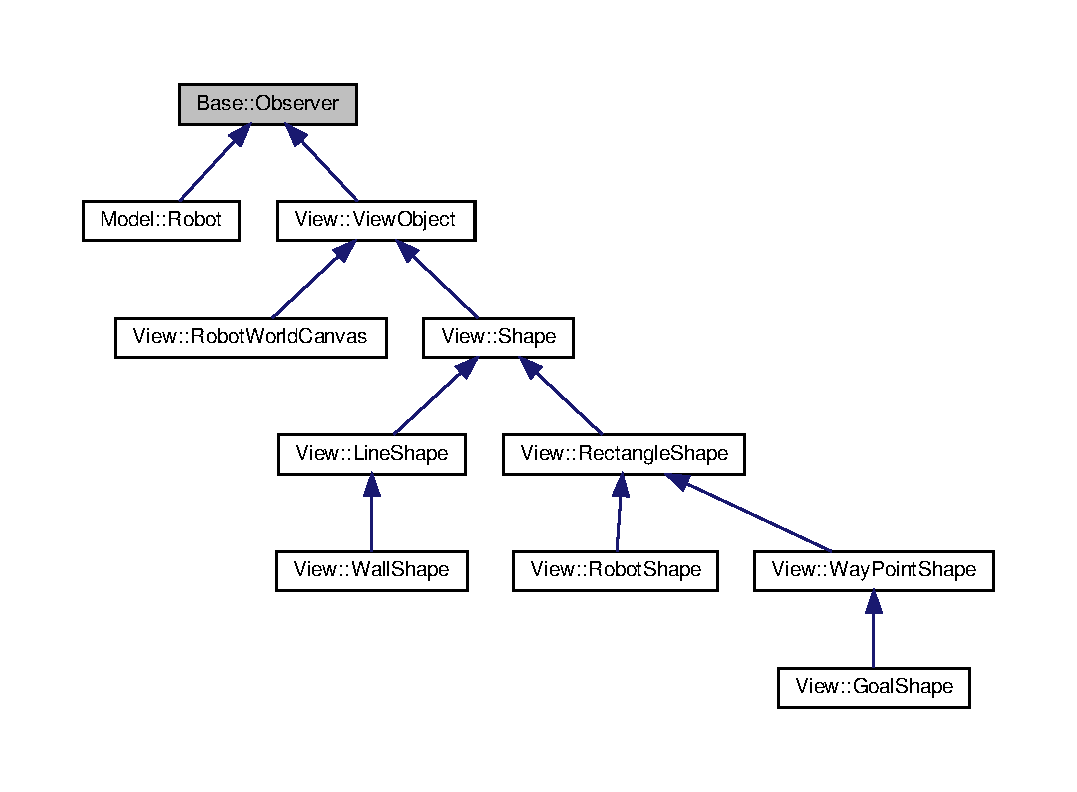
\includegraphics[width=350pt]{class_base_1_1_observer__inherit__graph}
\end{center}
\end{figure}
\subsection*{Public Member Functions}
\begin{Indent}{\bf Constructors and destructor}\par
\begin{DoxyCompactItemize}
\item 
{\bfseries Observer} ()\hypertarget{class_base_1_1_observer_a0b8f55248bb0b393ed760d50b7f58d21}{}\label{class_base_1_1_observer_a0b8f55248bb0b393ed760d50b7f58d21}

\item 
virtual {\bfseries $\sim$\+Observer} ()\hypertarget{class_base_1_1_observer_aca7a3c17bdc9d86a9f67519779baf2e9}{}\label{class_base_1_1_observer_aca7a3c17bdc9d86a9f67519779baf2e9}

\end{DoxyCompactItemize}
\end{Indent}
\begin{Indent}{\bf Operators}\par
\begin{DoxyCompactItemize}
\item 
bool \hyperlink{class_base_1_1_observer_aca74f78fc397401d5e90cd85193bd84c}{operator==} (const \hyperlink{class_base_1_1_observer}{Observer} \&a\+Observer) const 
\item 
bool \hyperlink{class_base_1_1_observer_aeabd57c2929d345f45132d4c0c1c6c58}{operator$<$} (const \hyperlink{class_base_1_1_observer}{Observer} \&a\+Observer) const 
\end{DoxyCompactItemize}
\end{Indent}
\begin{Indent}{\bf Observer functions}\par
\begin{DoxyCompactItemize}
\item 
virtual void \hyperlink{class_base_1_1_observer_a805cc1ddc6526d692af81d76ae29d802}{handle\+Notifications\+For} (\hyperlink{class_base_1_1_notifier}{Notifier} \&a\+Notifier)
\item 
virtual void \hyperlink{class_base_1_1_observer_a0646f881f6716ab7be41ecefa74b5071}{stop\+Handling\+Notifications\+For} (\hyperlink{class_base_1_1_notifier}{Notifier} \&a\+Notifier)
\item 
virtual void \hyperlink{class_base_1_1_observer_a37d00a5290a60aa9ab664af5d1642c3e}{handle\+Notification} ()=0
\end{DoxyCompactItemize}
\end{Indent}
\subsection*{Friends}
\begin{DoxyCompactItemize}
\item 
class {\bfseries Notifier}\hypertarget{class_base_1_1_observer_ac1a7d2e9a33255ac264c6abd1782cd8d}{}\label{class_base_1_1_observer_ac1a7d2e9a33255ac264c6abd1782cd8d}

\end{DoxyCompactItemize}


\subsection{Detailed Description}
The \hyperlink{class_base_1_1_observer}{Observer} class is part of a straight forward implementation of the Observer/\+Notifier pattern

\begin{DoxySeeAlso}{See also}
\hyperlink{class_base_1_1_notifier}{Notifier} 
\end{DoxySeeAlso}


\subsection{Member Function Documentation}
\index{Base\+::\+Observer@{Base\+::\+Observer}!handle\+Notification@{handle\+Notification}}
\index{handle\+Notification@{handle\+Notification}!Base\+::\+Observer@{Base\+::\+Observer}}
\subsubsection[{\texorpdfstring{handle\+Notification()=0}{handleNotification()=0}}]{\setlength{\rightskip}{0pt plus 5cm}virtual void Base\+::\+Observer\+::handle\+Notification (
\begin{DoxyParamCaption}
{}
\end{DoxyParamCaption}
)\hspace{0.3cm}{\ttfamily [pure virtual]}}\hypertarget{class_base_1_1_observer_a37d00a5290a60aa9ab664af5d1642c3e}{}\label{class_base_1_1_observer_a37d00a5290a60aa9ab664af5d1642c3e}
A \hyperlink{class_base_1_1_notifier}{Notifier} will call this function if this \hyperlink{class_base_1_1_observer}{Observer} will handle the notifications of that \hyperlink{class_base_1_1_notifier}{Notifier}. It is the responsibility of the \hyperlink{class_base_1_1_observer}{Observer} to filter any events it is interested in. 

Implemented in \hyperlink{class_model_1_1_robot_a7629555402fa8b55658d52fdc88ab889}{model\+::\+Robot}, \hyperlink{class_view_1_1_robot_world_canvas_af24f07e5484dbba2edd563c826694098}{View\+::\+Robot\+World\+Canvas}, \hyperlink{class_view_1_1_robot_shape_aa8e3a33d23b11a1f9c4580ff46d3d9f7}{View\+::\+Robot\+Shape}, \hyperlink{class_view_1_1_goal_shape_a881cfbfd4b3d6d3b37498e12d8291f6f}{View\+::\+Goal\+Shape}, \hyperlink{class_view_1_1_way_point_shape_a84f786f8027e91441c8197cdb56b3d5f}{View\+::\+Way\+Point\+Shape}, \hyperlink{class_view_1_1_rectangle_shape_acae95cb4b05d77196451520ee7d7ca9c}{View\+::\+Rectangle\+Shape}, and \hyperlink{class_view_1_1_line_shape_a21a183cd9f63130fe48497743c2c4abb}{View\+::\+Line\+Shape}.

\index{Base\+::\+Observer@{Base\+::\+Observer}!handle\+Notifications\+For@{handle\+Notifications\+For}}
\index{handle\+Notifications\+For@{handle\+Notifications\+For}!Base\+::\+Observer@{Base\+::\+Observer}}
\subsubsection[{\texorpdfstring{handle\+Notifications\+For(\+Notifier \&a\+Notifier)}{handleNotificationsFor(Notifier &aNotifier)}}]{\setlength{\rightskip}{0pt plus 5cm}void Base\+::\+Observer\+::handle\+Notifications\+For (
\begin{DoxyParamCaption}
\item[{{\bf Notifier} \&}]{a\+Notifier}
\end{DoxyParamCaption}
)\hspace{0.3cm}{\ttfamily [virtual]}}\hypertarget{class_base_1_1_observer_a805cc1ddc6526d692af81d76ae29d802}{}\label{class_base_1_1_observer_a805cc1ddc6526d692af81d76ae29d802}

\begin{DoxyParams}{Parameters}
{\em a\+Notifier} & The \hyperlink{class_base_1_1_notifier}{Notifier} this \hyperlink{class_base_1_1_observer}{Observer} will observe \\
\hline
\end{DoxyParams}
\index{Base\+::\+Observer@{Base\+::\+Observer}!operator$<$@{operator$<$}}
\index{operator$<$@{operator$<$}!Base\+::\+Observer@{Base\+::\+Observer}}
\subsubsection[{\texorpdfstring{operator$<$(const Observer \&a\+Observer) const }{operator<(const Observer &aObserver) const }}]{\setlength{\rightskip}{0pt plus 5cm}bool Base\+::\+Observer\+::operator$<$ (
\begin{DoxyParamCaption}
\item[{const {\bf Observer} \&}]{a\+Observer}
\end{DoxyParamCaption}
) const}\hypertarget{class_base_1_1_observer_aeabd57c2929d345f45132d4c0c1c6c58}{}\label{class_base_1_1_observer_aeabd57c2929d345f45132d4c0c1c6c58}
Compares the this pointer by default. \index{Base\+::\+Observer@{Base\+::\+Observer}!operator==@{operator==}}
\index{operator==@{operator==}!Base\+::\+Observer@{Base\+::\+Observer}}
\subsubsection[{\texorpdfstring{operator==(const Observer \&a\+Observer) const }{operator==(const Observer &aObserver) const }}]{\setlength{\rightskip}{0pt plus 5cm}bool Base\+::\+Observer\+::operator== (
\begin{DoxyParamCaption}
\item[{const {\bf Observer} \&}]{a\+Observer}
\end{DoxyParamCaption}
) const}\hypertarget{class_base_1_1_observer_aca74f78fc397401d5e90cd85193bd84c}{}\label{class_base_1_1_observer_aca74f78fc397401d5e90cd85193bd84c}
Compares the this pointer by default. \index{Base\+::\+Observer@{Base\+::\+Observer}!stop\+Handling\+Notifications\+For@{stop\+Handling\+Notifications\+For}}
\index{stop\+Handling\+Notifications\+For@{stop\+Handling\+Notifications\+For}!Base\+::\+Observer@{Base\+::\+Observer}}
\subsubsection[{\texorpdfstring{stop\+Handling\+Notifications\+For(\+Notifier \&a\+Notifier)}{stopHandlingNotificationsFor(Notifier &aNotifier)}}]{\setlength{\rightskip}{0pt plus 5cm}void Base\+::\+Observer\+::stop\+Handling\+Notifications\+For (
\begin{DoxyParamCaption}
\item[{{\bf Notifier} \&}]{a\+Notifier}
\end{DoxyParamCaption}
)\hspace{0.3cm}{\ttfamily [virtual]}}\hypertarget{class_base_1_1_observer_a0646f881f6716ab7be41ecefa74b5071}{}\label{class_base_1_1_observer_a0646f881f6716ab7be41ecefa74b5071}

\begin{DoxyParams}{Parameters}
{\em a\+Notifier} & The \hyperlink{class_base_1_1_notifier}{Notifier} this \hyperlink{class_base_1_1_observer}{Observer} will not observe anymore \\
\hline
\end{DoxyParams}


The documentation for this class was generated from the following files\+:\begin{DoxyCompactItemize}
\item 
/home/hqnders/\+Documents/robotworld/src/Observer.\+hpp\item 
/home/hqnders/\+Documents/robotworld/src/Observer.\+cpp\end{DoxyCompactItemize}

\hypertarget{class_base_1_1_queue}{}\section{Base\+:\+:Queue$<$ Queue\+Content\+Type $>$ Class Template Reference}
\label{class_base_1_1_queue}\index{Base\+::\+Queue$<$ Queue\+Content\+Type $>$@{Base\+::\+Queue$<$ Queue\+Content\+Type $>$}}
\subsection*{Public Member Functions}
\begin{DoxyCompactItemize}
\item 
void {\bfseries enqueue} (const Queue\+Content\+Type \&an\+Element)\hypertarget{class_base_1_1_queue_a2f737b5dc4b04016bc529fdac46a59a2}{}\label{class_base_1_1_queue_a2f737b5dc4b04016bc529fdac46a59a2}

\item 
Queue\+Content\+Type {\bfseries dequeue} ()\hypertarget{class_base_1_1_queue_a256b99ec524acf877586ae7450dfcb13}{}\label{class_base_1_1_queue_a256b99ec524acf877586ae7450dfcb13}

\item 
size\+\_\+t {\bfseries size} () const \hypertarget{class_base_1_1_queue_a1facbc77b95d2dc9c897f2893604b816}{}\label{class_base_1_1_queue_a1facbc77b95d2dc9c897f2893604b816}

\end{DoxyCompactItemize}


The documentation for this class was generated from the following file\+:\begin{DoxyCompactItemize}
\item 
/home/hqnders/\+Documents/robotworld/src/Queue.\+hpp\end{DoxyCompactItemize}

\hypertarget{class_view_1_1_rectangle_shape}{}\section{View\+:\+:Rectangle\+Shape Class Reference}
\label{class_view_1_1_rectangle_shape}\index{View\+::\+Rectangle\+Shape@{View\+::\+Rectangle\+Shape}}


Inheritance diagram for View\+:\+:Rectangle\+Shape\+:
\nopagebreak
\begin{figure}[H]
\begin{center}
\leavevmode
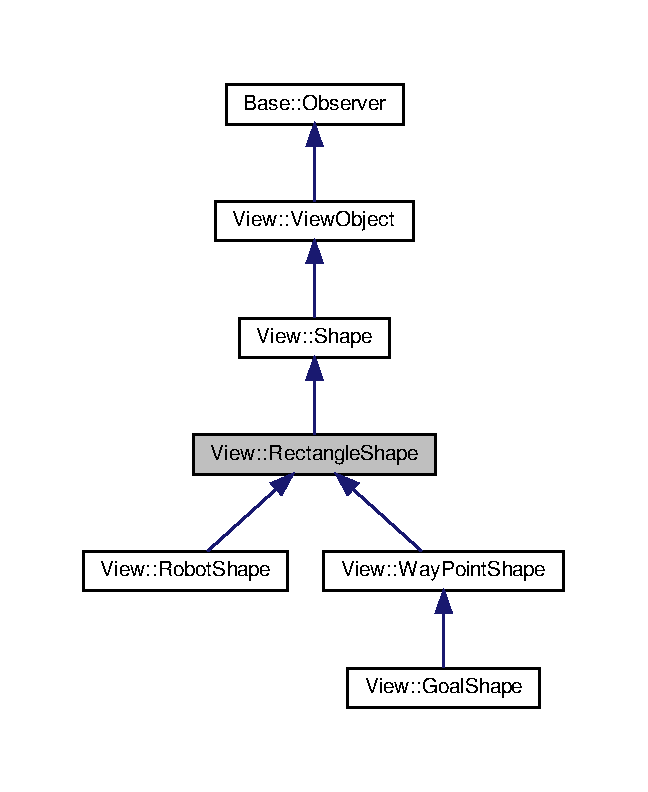
\includegraphics[width=311pt]{class_view_1_1_rectangle_shape__inherit__graph}
\end{center}
\end{figure}


Collaboration diagram for View\+:\+:Rectangle\+Shape\+:
\nopagebreak
\begin{figure}[H]
\begin{center}
\leavevmode
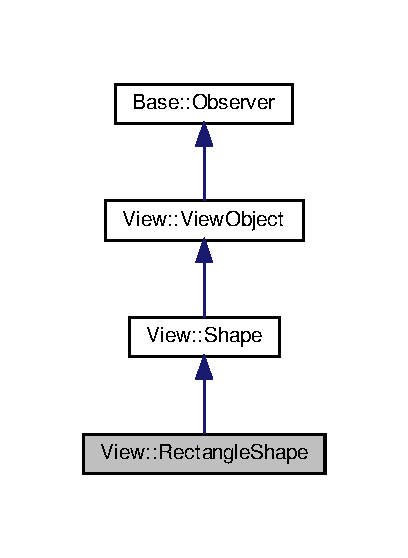
\includegraphics[width=196pt]{class_view_1_1_rectangle_shape__coll__graph}
\end{center}
\end{figure}
\subsection*{Public Member Functions}
\begin{DoxyCompactItemize}
\item 
{\bfseries Rectangle\+Shape} (const std\+::string \&a\+Title=\char`\"{}\char`\"{})\hypertarget{class_view_1_1_rectangle_shape_a6fc6a32c159acc4ef318564996fa0965}{}\label{class_view_1_1_rectangle_shape_a6fc6a32c159acc4ef318564996fa0965}

\item 
{\bfseries Rectangle\+Shape} (const Point \&a\+Centre\+Point, const std\+::string \&a\+Title=\char`\"{}\char`\"{}, int a\+Border\+Width=2, int a\+Spacing=2)\hypertarget{class_view_1_1_rectangle_shape_a9625cfce67d2df4c22014467a3dbc0e0}{}\label{class_view_1_1_rectangle_shape_a9625cfce67d2df4c22014467a3dbc0e0}

\item 
{\bfseries Rectangle\+Shape} (model\+::\+model\+Object\+Ptr a\+model\+Object, const Point \&a\+Centre\+Point, const std\+::string \&a\+Title=\char`\"{}\char`\"{}, int a\+Border\+Width=2, int a\+Spacing=2)\hypertarget{class_view_1_1_rectangle_shape_a3203649d35ff84e9b5523d16832c757e}{}\label{class_view_1_1_rectangle_shape_a3203649d35ff84e9b5523d16832c757e}

\item 
\hyperlink{class_view_1_1_rectangle_shape}{Rectangle\+Shape} \& {\bfseries operator=} (const \hyperlink{class_view_1_1_rectangle_shape}{Rectangle\+Shape} \&a\+Rectangle\+Shape)\hypertarget{class_view_1_1_rectangle_shape_a7c1339a9ae1096201bfdc9b8a0802a48}{}\label{class_view_1_1_rectangle_shape_a7c1339a9ae1096201bfdc9b8a0802a48}

\item 
virtual bool \hyperlink{class_view_1_1_rectangle_shape_a69be3838db55e8557e6cb1e767ed0aab}{is\+Border\+Point} (const Point a\+Point, int a\+Radius=3) const 
\item 
virtual Point {\bfseries get\+Centre} () const \hypertarget{class_view_1_1_rectangle_shape_a075d237a4c4bad46346e9305fd9f60d7}{}\label{class_view_1_1_rectangle_shape_a075d237a4c4bad46346e9305fd9f60d7}

\item 
virtual void {\bfseries set\+Centre} (const Point \&a\+Point)\hypertarget{class_view_1_1_rectangle_shape_a905817abb1294f0e83f1ecdb065cc994}{}\label{class_view_1_1_rectangle_shape_a905817abb1294f0e83f1ecdb065cc994}

\item 
std\+::string {\bfseries get\+Title} () const \hypertarget{class_view_1_1_rectangle_shape_a6f431ce0f2f8436c8071eb7d07f198aa}{}\label{class_view_1_1_rectangle_shape_a6f431ce0f2f8436c8071eb7d07f198aa}

\item 
virtual std\+::string {\bfseries get\+Normal\+Colour} () const \hypertarget{class_view_1_1_rectangle_shape_a1014ef91f3ffb2b7da225293051cda8a}{}\label{class_view_1_1_rectangle_shape_a1014ef91f3ffb2b7da225293051cda8a}

\item 
virtual std\+::string {\bfseries get\+Selection\+Colour} () const \hypertarget{class_view_1_1_rectangle_shape_a2d0161c7d5a84cf2305b41f8b14f7573}{}\label{class_view_1_1_rectangle_shape_a2d0161c7d5a84cf2305b41f8b14f7573}

\item 
virtual std\+::string {\bfseries get\+Activation\+Colour} () const \hypertarget{class_view_1_1_rectangle_shape_a30ef8c82bf9c40d0f39ce9568c7027f7}{}\label{class_view_1_1_rectangle_shape_a30ef8c82bf9c40d0f39ce9568c7027f7}

\item 
void {\bfseries set\+Title} (const std\+::string \&a\+Title)\hypertarget{class_view_1_1_rectangle_shape_a21019b56d4ddb7d582e7bd3ee13f8973}{}\label{class_view_1_1_rectangle_shape_a21019b56d4ddb7d582e7bd3ee13f8973}

\item 
virtual Size {\bfseries get\+Size} () const \hypertarget{class_view_1_1_rectangle_shape_abbc036fe705e1766ec6294707eac1567}{}\label{class_view_1_1_rectangle_shape_abbc036fe705e1766ec6294707eac1567}

\item 
virtual void {\bfseries set\+Size} (const Size \&a\+Size)\hypertarget{class_view_1_1_rectangle_shape_a1750f2d2258a33f149764d2df471a7ae}{}\label{class_view_1_1_rectangle_shape_a1750f2d2258a33f149764d2df471a7ae}

\item 
int {\bfseries get\+Border\+Width} () const \hypertarget{class_view_1_1_rectangle_shape_acc3ec065295ec50ae74e1a6546ea97dc}{}\label{class_view_1_1_rectangle_shape_acc3ec065295ec50ae74e1a6546ea97dc}

\item 
void {\bfseries set\+Border\+Width} (int a\+Border\+Width)\hypertarget{class_view_1_1_rectangle_shape_a5cc335ae000fa88ef759b89a8b83acd0}{}\label{class_view_1_1_rectangle_shape_a5cc335ae000fa88ef759b89a8b83acd0}

\item 
int {\bfseries get\+Spacing} () const \hypertarget{class_view_1_1_rectangle_shape_a892ec0b500eaa885ee4514d1775a37e9}{}\label{class_view_1_1_rectangle_shape_a892ec0b500eaa885ee4514d1775a37e9}

\item 
void {\bfseries set\+Spacing} (int a\+Spacing)\hypertarget{class_view_1_1_rectangle_shape_aa1d0774ba0de3aeb2acdc6b4af528fd5}{}\label{class_view_1_1_rectangle_shape_aa1d0774ba0de3aeb2acdc6b4af528fd5}

\item 
virtual void \hyperlink{class_view_1_1_rectangle_shape_a6e075b3fda71d5dd4fbd3f3f9ff42126}{handle\+Activated} ()
\item 
virtual void \hyperlink{class_view_1_1_rectangle_shape_a15a3cd81166a65e5734b79c87552db00}{handle\+Selection} ()
\end{DoxyCompactItemize}
\begin{Indent}{\bf Observer functions}\par
\begin{DoxyCompactItemize}
\item 
virtual void \hyperlink{class_view_1_1_rectangle_shape_acae95cb4b05d77196451520ee7d7ca9c}{handle\+Notification} ()
\end{DoxyCompactItemize}
\end{Indent}
\begin{Indent}{\bf Pure virtual abstract Shape functions}\par
\begin{DoxyCompactItemize}
\item 
virtual void {\bfseries draw} (wx\+DC \&dc)\hypertarget{class_view_1_1_rectangle_shape_a430ce6f93a932205861ec0327df3ca42}{}\label{class_view_1_1_rectangle_shape_a430ce6f93a932205861ec0327df3ca42}

\item 
virtual bool \hyperlink{class_view_1_1_rectangle_shape_ac736dfe69f1a3633696d8c663cd49b51}{occupies} (const Point \&a\+Point) const 
\end{DoxyCompactItemize}
\end{Indent}
\begin{Indent}{\bf Debug functions}\par
\begin{DoxyCompactItemize}
\item 
virtual std\+::string \hyperlink{class_view_1_1_rectangle_shape_a82517a7fb6b1b0331efaa79f306ecc38}{as\+String} () const 
\item 
virtual std\+::string \hyperlink{class_view_1_1_rectangle_shape_ae46b92ba72ec4a590afbd106ced79c98}{as\+Debug\+String} () const 
\end{DoxyCompactItemize}
\end{Indent}
\subsection*{Protected Attributes}
\begin{DoxyCompactItemize}
\item 
Point {\bfseries centre}\hypertarget{class_view_1_1_rectangle_shape_a12930d710b0629b49c95c86d686291a3}{}\label{class_view_1_1_rectangle_shape_a12930d710b0629b49c95c86d686291a3}

\item 
Size {\bfseries size}\hypertarget{class_view_1_1_rectangle_shape_a92563881c24a730b99d600b39558ebfc}{}\label{class_view_1_1_rectangle_shape_a92563881c24a730b99d600b39558ebfc}

\item 
std\+::string {\bfseries title}\hypertarget{class_view_1_1_rectangle_shape_af9f808c588d4c618d857dcd46e27073f}{}\label{class_view_1_1_rectangle_shape_af9f808c588d4c618d857dcd46e27073f}

\item 
Size {\bfseries title\+Size}\hypertarget{class_view_1_1_rectangle_shape_aff10ae7e56d55aca3f4accd7386e6e4f}{}\label{class_view_1_1_rectangle_shape_aff10ae7e56d55aca3f4accd7386e6e4f}

\item 
int {\bfseries border\+Width}\hypertarget{class_view_1_1_rectangle_shape_ac32ad0276db89433370ad4a50752b734}{}\label{class_view_1_1_rectangle_shape_ac32ad0276db89433370ad4a50752b734}

\item 
int {\bfseries spacing}\hypertarget{class_view_1_1_rectangle_shape_ab2330833ac41ecb5233ce20728450a7b}{}\label{class_view_1_1_rectangle_shape_ab2330833ac41ecb5233ce20728450a7b}

\end{DoxyCompactItemize}
\subsection*{Additional Inherited Members}


\subsection{Member Function Documentation}
\index{View\+::\+Rectangle\+Shape@{View\+::\+Rectangle\+Shape}!as\+Debug\+String@{as\+Debug\+String}}
\index{as\+Debug\+String@{as\+Debug\+String}!View\+::\+Rectangle\+Shape@{View\+::\+Rectangle\+Shape}}
\subsubsection[{\texorpdfstring{as\+Debug\+String() const }{asDebugString() const }}]{\setlength{\rightskip}{0pt plus 5cm}std\+::string View\+::\+Rectangle\+Shape\+::as\+Debug\+String (
\begin{DoxyParamCaption}
{}
\end{DoxyParamCaption}
) const\hspace{0.3cm}{\ttfamily [virtual]}}\hypertarget{class_view_1_1_rectangle_shape_ae46b92ba72ec4a590afbd106ced79c98}{}\label{class_view_1_1_rectangle_shape_ae46b92ba72ec4a590afbd106ced79c98}
Returns a description of the object with all data of the object usable for debugging 

Reimplemented from \hyperlink{class_view_1_1_shape_a47a54c2594bad3a5a26ed5aabf9c3f7c}{View\+::\+Shape}.



Reimplemented in \hyperlink{class_view_1_1_robot_shape_afb69a3cb5c895002b054807d26291579}{View\+::\+Robot\+Shape}, \hyperlink{class_view_1_1_way_point_shape_a0f21e281b69fe62eb8728ad5dc28fce6}{View\+::\+Way\+Point\+Shape}, and \hyperlink{class_view_1_1_goal_shape_a7d88c0780ae52278bacb44f4a6c79da5}{View\+::\+Goal\+Shape}.

\index{View\+::\+Rectangle\+Shape@{View\+::\+Rectangle\+Shape}!as\+String@{as\+String}}
\index{as\+String@{as\+String}!View\+::\+Rectangle\+Shape@{View\+::\+Rectangle\+Shape}}
\subsubsection[{\texorpdfstring{as\+String() const }{asString() const }}]{\setlength{\rightskip}{0pt plus 5cm}std\+::string View\+::\+Rectangle\+Shape\+::as\+String (
\begin{DoxyParamCaption}
{}
\end{DoxyParamCaption}
) const\hspace{0.3cm}{\ttfamily [virtual]}}\hypertarget{class_view_1_1_rectangle_shape_a82517a7fb6b1b0331efaa79f306ecc38}{}\label{class_view_1_1_rectangle_shape_a82517a7fb6b1b0331efaa79f306ecc38}
Returns a 1-\/line description of the object 

Reimplemented from \hyperlink{class_view_1_1_shape_a54231a2190a7244fdbd1b66900acf162}{View\+::\+Shape}.



Reimplemented in \hyperlink{class_view_1_1_robot_shape_a2af7fa2dfdf390213a921751fb144afa}{View\+::\+Robot\+Shape}, \hyperlink{class_view_1_1_way_point_shape_a89bbc1a878732d81245c5b5b6c5f035a}{View\+::\+Way\+Point\+Shape}, and \hyperlink{class_view_1_1_goal_shape_a7f6c2c9c9502d264657a0b688e3d5e86}{View\+::\+Goal\+Shape}.

\index{View\+::\+Rectangle\+Shape@{View\+::\+Rectangle\+Shape}!handle\+Activated@{handle\+Activated}}
\index{handle\+Activated@{handle\+Activated}!View\+::\+Rectangle\+Shape@{View\+::\+Rectangle\+Shape}}
\subsubsection[{\texorpdfstring{handle\+Activated()}{handleActivated()}}]{\setlength{\rightskip}{0pt plus 5cm}void View\+::\+Rectangle\+Shape\+::handle\+Activated (
\begin{DoxyParamCaption}
{}
\end{DoxyParamCaption}
)\hspace{0.3cm}{\ttfamily [virtual]}}\hypertarget{class_view_1_1_rectangle_shape_a6e075b3fda71d5dd4fbd3f3f9ff42126}{}\label{class_view_1_1_rectangle_shape_a6e075b3fda71d5dd4fbd3f3f9ff42126}
This function is called by the \hyperlink{class_view_1_1_robot_world_canvas}{Robot\+World\+Canvas} if enable\+Activation is set for the \hyperlink{class_view_1_1_robot_world_canvas}{Robot\+World\+Canvas}. If this is not the desired behaviour override Robot\+World\+Canvas\+::handle\+Item\+Activated in a derived class. 

Reimplemented from \hyperlink{class_view_1_1_shape_ac128288b584db6de840f7ec20493aafd}{View\+::\+Shape}.



Reimplemented in \hyperlink{class_view_1_1_robot_shape_ab07702949d9d374331a17db4759f0762}{View\+::\+Robot\+Shape}.

\index{View\+::\+Rectangle\+Shape@{View\+::\+Rectangle\+Shape}!handle\+Notification@{handle\+Notification}}
\index{handle\+Notification@{handle\+Notification}!View\+::\+Rectangle\+Shape@{View\+::\+Rectangle\+Shape}}
\subsubsection[{\texorpdfstring{handle\+Notification()}{handleNotification()}}]{\setlength{\rightskip}{0pt plus 5cm}virtual void View\+::\+Rectangle\+Shape\+::handle\+Notification (
\begin{DoxyParamCaption}
{}
\end{DoxyParamCaption}
)\hspace{0.3cm}{\ttfamily [inline]}, {\ttfamily [virtual]}}\hypertarget{class_view_1_1_rectangle_shape_acae95cb4b05d77196451520ee7d7ca9c}{}\label{class_view_1_1_rectangle_shape_acae95cb4b05d77196451520ee7d7ca9c}
A Notifier will call this function if this Observer will handle the notifications of that Notifier. It is the responsibility of the Observer to filter any events it is interested in. 

Implements \hyperlink{class_base_1_1_observer_a37d00a5290a60aa9ab664af5d1642c3e}{Base\+::\+Observer}.



Reimplemented in \hyperlink{class_view_1_1_robot_shape_aa8e3a33d23b11a1f9c4580ff46d3d9f7}{View\+::\+Robot\+Shape}, \hyperlink{class_view_1_1_goal_shape_a881cfbfd4b3d6d3b37498e12d8291f6f}{View\+::\+Goal\+Shape}, and \hyperlink{class_view_1_1_way_point_shape_a84f786f8027e91441c8197cdb56b3d5f}{View\+::\+Way\+Point\+Shape}.

\index{View\+::\+Rectangle\+Shape@{View\+::\+Rectangle\+Shape}!handle\+Selection@{handle\+Selection}}
\index{handle\+Selection@{handle\+Selection}!View\+::\+Rectangle\+Shape@{View\+::\+Rectangle\+Shape}}
\subsubsection[{\texorpdfstring{handle\+Selection()}{handleSelection()}}]{\setlength{\rightskip}{0pt plus 5cm}void View\+::\+Rectangle\+Shape\+::handle\+Selection (
\begin{DoxyParamCaption}
{}
\end{DoxyParamCaption}
)\hspace{0.3cm}{\ttfamily [virtual]}}\hypertarget{class_view_1_1_rectangle_shape_a15a3cd81166a65e5734b79c87552db00}{}\label{class_view_1_1_rectangle_shape_a15a3cd81166a65e5734b79c87552db00}
This function is called by the \hyperlink{class_view_1_1_robot_world_canvas}{Robot\+World\+Canvas} if enable\+Selection is set for the \hyperlink{class_view_1_1_robot_world_canvas}{Robot\+World\+Canvas}. If this is not the desired behaviour override Robot\+World\+Canvas\+::handle\+Selection\+Changed in a derived class. 

Reimplemented from \hyperlink{class_view_1_1_shape_a62035e3329fede659614b5ce2060a0f3}{View\+::\+Shape}.



Reimplemented in \hyperlink{class_view_1_1_robot_shape_a8983c43b4ec8cd9eda0f4e32a8f69b19}{View\+::\+Robot\+Shape}.

\index{View\+::\+Rectangle\+Shape@{View\+::\+Rectangle\+Shape}!is\+Border\+Point@{is\+Border\+Point}}
\index{is\+Border\+Point@{is\+Border\+Point}!View\+::\+Rectangle\+Shape@{View\+::\+Rectangle\+Shape}}
\subsubsection[{\texorpdfstring{is\+Border\+Point(const Point a\+Point, int a\+Radius=3) const }{isBorderPoint(const Point aPoint, int aRadius=3) const }}]{\setlength{\rightskip}{0pt plus 5cm}bool View\+::\+Rectangle\+Shape\+::is\+Border\+Point (
\begin{DoxyParamCaption}
\item[{const Point}]{a\+Point, }
\item[{int}]{a\+Radius = {\ttfamily 3}}
\end{DoxyParamCaption}
) const\hspace{0.3cm}{\ttfamily [virtual]}}\hypertarget{class_view_1_1_rectangle_shape_a69be3838db55e8557e6cb1e767ed0aab}{}\label{class_view_1_1_rectangle_shape_a69be3838db55e8557e6cb1e767ed0aab}
\begin{DoxyReturn}{Returns}
True if the point is on the border of the shape 
\end{DoxyReturn}
\index{View\+::\+Rectangle\+Shape@{View\+::\+Rectangle\+Shape}!occupies@{occupies}}
\index{occupies@{occupies}!View\+::\+Rectangle\+Shape@{View\+::\+Rectangle\+Shape}}
\subsubsection[{\texorpdfstring{occupies(const Point \&a\+Point) const }{occupies(const Point &aPoint) const }}]{\setlength{\rightskip}{0pt plus 5cm}bool View\+::\+Rectangle\+Shape\+::occupies (
\begin{DoxyParamCaption}
\item[{const Point \&}]{a\+Point}
\end{DoxyParamCaption}
) const\hspace{0.3cm}{\ttfamily [virtual]}}\hypertarget{class_view_1_1_rectangle_shape_ac736dfe69f1a3633696d8c663cd49b51}{}\label{class_view_1_1_rectangle_shape_ac736dfe69f1a3633696d8c663cd49b51}

\begin{DoxyParams}{Parameters}
{\em a\+Point} & \\
\hline
\end{DoxyParams}
\begin{DoxyReturn}{Returns}
True if the point is in the shape 
\end{DoxyReturn}


Implements \hyperlink{class_view_1_1_shape_a7a202614a593376dcfae7baf892604b1}{View\+::\+Shape}.



Reimplemented in \hyperlink{class_view_1_1_robot_shape_aff3acf7b0326d17f5cabdc19c7164095}{View\+::\+Robot\+Shape}.



The documentation for this class was generated from the following files\+:\begin{DoxyCompactItemize}
\item 
/home/hqnders/\+Documents/robotworld/src/Rectangle\+Shape.\+hpp\item 
/home/hqnders/\+Documents/robotworld/src/Rectangle\+Shape.\+cpp\end{DoxyCompactItemize}

\hypertarget{class_messaging_1_1_request_handler}{}\section{Messaging\+:\+:Request\+Handler Class Reference}
\label{class_messaging_1_1_request_handler}\index{Messaging\+::\+Request\+Handler@{Messaging\+::\+Request\+Handler}}


{\ttfamily \#include $<$Message\+Handler.\+hpp$>$}



Inheritance diagram for Messaging\+:\+:Request\+Handler\+:
\nopagebreak
\begin{figure}[H]
\begin{center}
\leavevmode
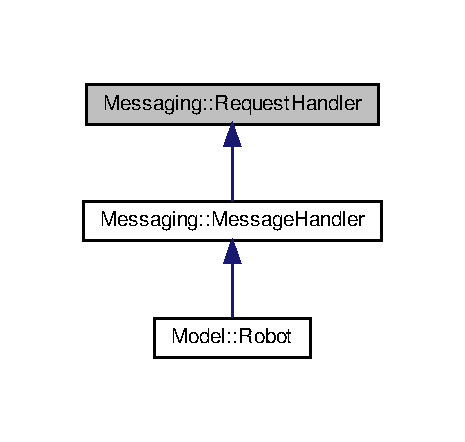
\includegraphics[width=223pt]{class_messaging_1_1_request_handler__inherit__graph}
\end{center}
\end{figure}
\subsection*{Public Member Functions}
\begin{DoxyCompactItemize}
\item 
virtual void \hyperlink{class_messaging_1_1_request_handler_afa23f0ab94ae851a487173a5087da898}{handle\+Request} (\hyperlink{struct_messaging_1_1_message}{Message} \&a\+Message)=0
\end{DoxyCompactItemize}


\subsection{Detailed Description}
Base server interface for handling remote requests Classes derived from this interface can serve as server in the Messaging protocol by implementing this interface. 

\subsection{Member Function Documentation}
\index{Messaging\+::\+Request\+Handler@{Messaging\+::\+Request\+Handler}!handle\+Request@{handle\+Request}}
\index{handle\+Request@{handle\+Request}!Messaging\+::\+Request\+Handler@{Messaging\+::\+Request\+Handler}}
\subsubsection[{\texorpdfstring{handle\+Request(\+Message \&a\+Message)=0}{handleRequest(Message &aMessage)=0}}]{\setlength{\rightskip}{0pt plus 5cm}virtual void Messaging\+::\+Request\+Handler\+::handle\+Request (
\begin{DoxyParamCaption}
\item[{{\bf Message} \&}]{a\+Message}
\end{DoxyParamCaption}
)\hspace{0.3cm}{\ttfamily [pure virtual]}}\hypertarget{class_messaging_1_1_request_handler_afa23f0ab94ae851a487173a5087da898}{}\label{class_messaging_1_1_request_handler_afa23f0ab94ae851a487173a5087da898}
After this function is called a\+Message is returned as response to the requesting client, i.\+e. it should contain the result/response of/to the request.


\begin{DoxyParams}{Parameters}
{\em a\+Message} & \\
\hline
\end{DoxyParams}


Implemented in \hyperlink{class_model_1_1_robot_a5b52eb37c4e11850c3f60263599bd79c}{model\+::\+Robot}.



The documentation for this class was generated from the following file\+:\begin{DoxyCompactItemize}
\item 
/home/hqnders/\+Documents/robotworld/src/Message\+Handler.\+hpp\end{DoxyCompactItemize}

\hypertarget{class_messaging_1_1_response_handler}{}\section{Messaging\+:\+:Response\+Handler Class Reference}
\label{class_messaging_1_1_response_handler}\index{Messaging\+::\+Response\+Handler@{Messaging\+::\+Response\+Handler}}


{\ttfamily \#include $<$Message\+Handler.\+hpp$>$}



Inheritance diagram for Messaging\+:\+:Response\+Handler\+:
\nopagebreak
\begin{figure}[H]
\begin{center}
\leavevmode
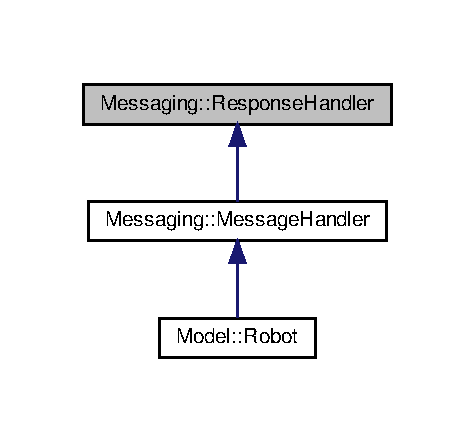
\includegraphics[width=228pt]{class_messaging_1_1_response_handler__inherit__graph}
\end{center}
\end{figure}
\subsection*{Public Member Functions}
\begin{DoxyCompactItemize}
\item 
virtual void \hyperlink{class_messaging_1_1_response_handler_a13c456a994ef15b4f7be7beed4e2f91f}{handle\+Response} (const \hyperlink{struct_messaging_1_1_message}{Message} \&a\+Message)=0
\end{DoxyCompactItemize}


\subsection{Detailed Description}
Base client interface for handling remote responses Classes derived from this interface can serve as client in the Messaging protocol by implementing this interface. 

\subsection{Member Function Documentation}
\index{Messaging\+::\+Response\+Handler@{Messaging\+::\+Response\+Handler}!handle\+Response@{handle\+Response}}
\index{handle\+Response@{handle\+Response}!Messaging\+::\+Response\+Handler@{Messaging\+::\+Response\+Handler}}
\subsubsection[{\texorpdfstring{handle\+Response(const Message \&a\+Message)=0}{handleResponse(const Message &aMessage)=0}}]{\setlength{\rightskip}{0pt plus 5cm}virtual void Messaging\+::\+Response\+Handler\+::handle\+Response (
\begin{DoxyParamCaption}
\item[{const {\bf Message} \&}]{a\+Message}
\end{DoxyParamCaption}
)\hspace{0.3cm}{\ttfamily [pure virtual]}}\hypertarget{class_messaging_1_1_response_handler_a13c456a994ef15b4f7be7beed4e2f91f}{}\label{class_messaging_1_1_response_handler_a13c456a994ef15b4f7be7beed4e2f91f}
The given argument contains the result/response of/to a previous request.


\begin{DoxyParams}{Parameters}
{\em a\+Message} & \\
\hline
\end{DoxyParams}


Implemented in \hyperlink{class_model_1_1_robot_afa5fb42fca43fdfedb08d3a7cb38c037}{model\+::\+Robot}.



The documentation for this class was generated from the following file\+:\begin{DoxyCompactItemize}
\item 
/home/hqnders/\+Documents/robotworld/src/Message\+Handler.\+hpp\end{DoxyCompactItemize}

\hypertarget{class_model_1_1_robot}{}\section{model\+:\+:Robot Class Reference}
\label{class_model_1_1_robot}\index{model\+::\+Robot@{model\+::\+Robot}}


Inheritance diagram for model\+:\+:Robot\+:
\nopagebreak
\begin{figure}[H]
\begin{center}
\leavevmode
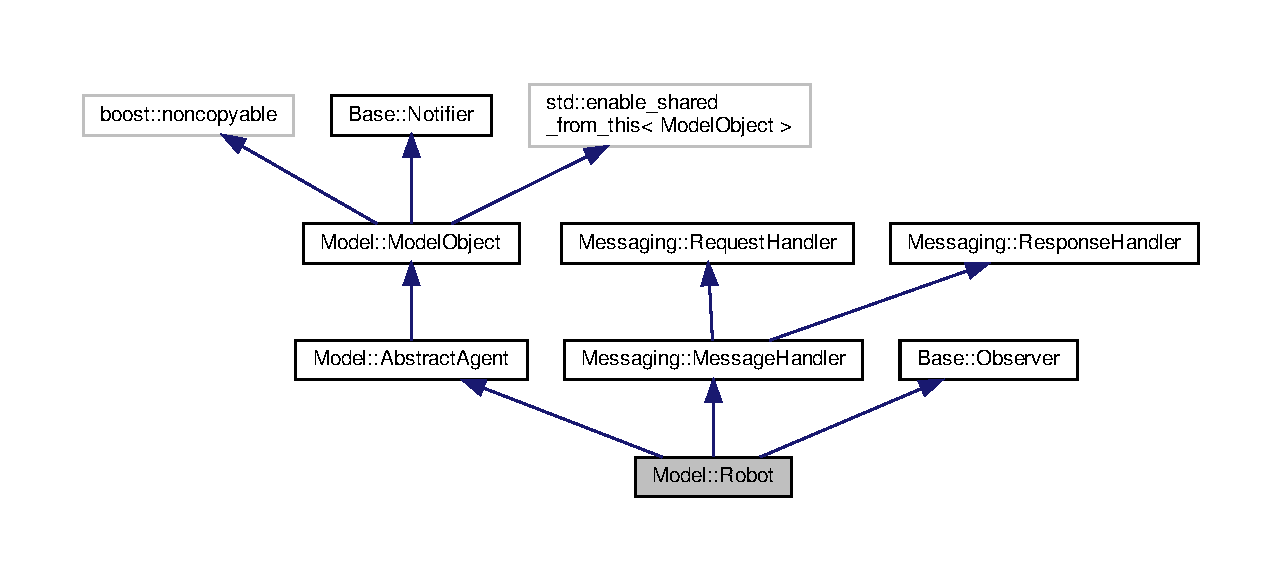
\includegraphics[width=350pt]{class_model_1_1_robot__inherit__graph}
\end{center}
\end{figure}


Collaboration diagram for model\+:\+:Robot\+:
\nopagebreak
\begin{figure}[H]
\begin{center}
\leavevmode
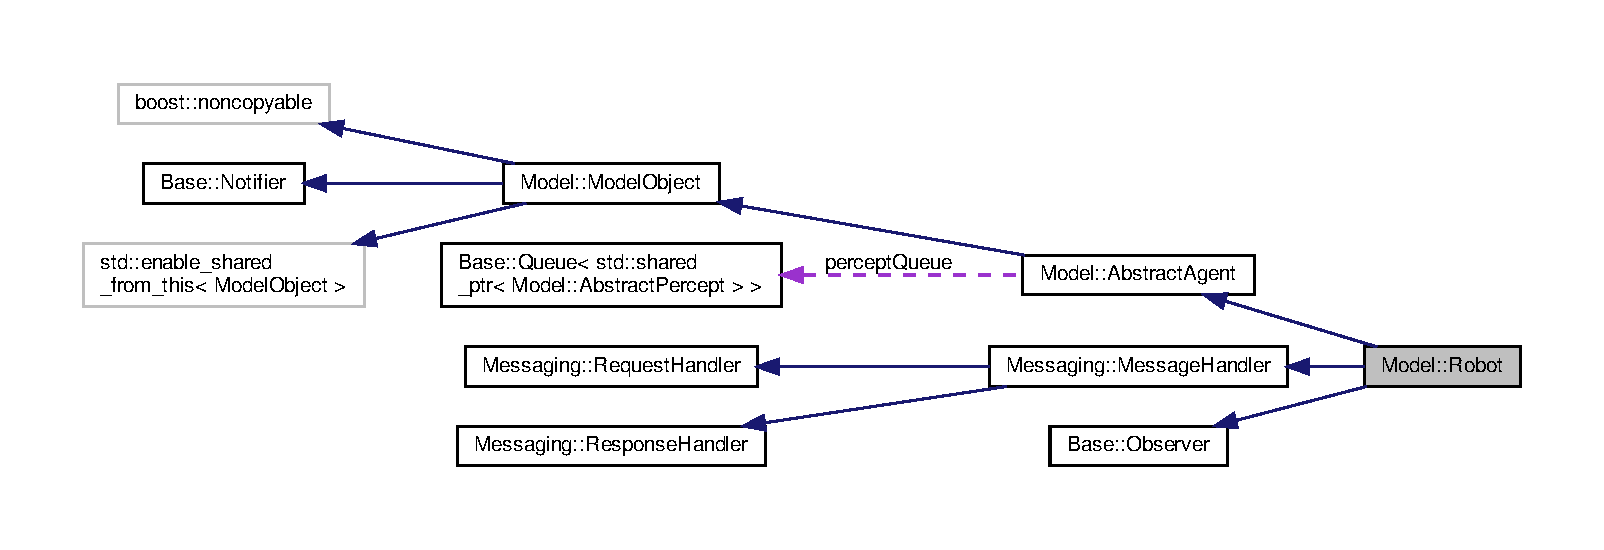
\includegraphics[width=350pt]{class_model_1_1_robot__coll__graph}
\end{center}
\end{figure}
\subsection*{Public Member Functions}
\begin{DoxyCompactItemize}
\item 
{\bfseries Robot} (const std\+::string \&a\+Name)\hypertarget{class_model_1_1_robot_a9fb211152f3e75c65eafd1550e90203f}{}\label{class_model_1_1_robot_a9fb211152f3e75c65eafd1550e90203f}

\item 
{\bfseries Robot} (const std\+::string \&a\+Name, const Point \&a\+Position)\hypertarget{class_model_1_1_robot_ac7afa4c9bc8982bd7e5918ed4c9173d2}{}\label{class_model_1_1_robot_ac7afa4c9bc8982bd7e5918ed4c9173d2}

\item 
std\+::string {\bfseries get\+Name} () const \hypertarget{class_model_1_1_robot_acbaa390189fe54d71c5ca1db809f10b0}{}\label{class_model_1_1_robot_acbaa390189fe54d71c5ca1db809f10b0}

\item 
void {\bfseries set\+Name} (const std\+::string \&a\+Name, bool a\+Notify\+Observers=true)\hypertarget{class_model_1_1_robot_ac39ad2cbd403962eebe60fd9dd4a1171}{}\label{class_model_1_1_robot_ac39ad2cbd403962eebe60fd9dd4a1171}

\item 
Size {\bfseries get\+Size} () const \hypertarget{class_model_1_1_robot_add846e39a98489592f07b456a06396db}{}\label{class_model_1_1_robot_add846e39a98489592f07b456a06396db}

\item 
void {\bfseries set\+Size} (const Size \&a\+Size, bool a\+Notify\+Observers=true)\hypertarget{class_model_1_1_robot_aa9053536ee4aa3c58883f1fe14d46c1f}{}\label{class_model_1_1_robot_aa9053536ee4aa3c58883f1fe14d46c1f}

\item 
Point {\bfseries get\+Position} () const \hypertarget{class_model_1_1_robot_a02a103f767306bce47f60127ceddf171}{}\label{class_model_1_1_robot_a02a103f767306bce47f60127ceddf171}

\item 
void {\bfseries set\+Position} (const Point \&a\+Position, bool a\+Notify\+Observers=true)\hypertarget{class_model_1_1_robot_a2d983199228926b70bc2dfa4dbbab006}{}\label{class_model_1_1_robot_a2d983199228926b70bc2dfa4dbbab006}

\item 
\hyperlink{class_model_1_1_bounded_vector}{Bounded\+Vector} {\bfseries get\+Front} () const \hypertarget{class_model_1_1_robot_a85ab146591702b24ab8bd9b2ff960a2f}{}\label{class_model_1_1_robot_a85ab146591702b24ab8bd9b2ff960a2f}

\item 
void {\bfseries set\+Front} (const \hyperlink{class_model_1_1_bounded_vector}{Bounded\+Vector} \&a\+Vector, bool a\+Notify\+Observers=true)\hypertarget{class_model_1_1_robot_ad61c7c66fc588a7ba017cbb1f0045e2f}{}\label{class_model_1_1_robot_ad61c7c66fc588a7ba017cbb1f0045e2f}

\item 
float {\bfseries get\+Speed} () const \hypertarget{class_model_1_1_robot_a134d8fa080a68cc524f386c8662be03e}{}\label{class_model_1_1_robot_a134d8fa080a68cc524f386c8662be03e}

\item 
void {\bfseries set\+Speed} (float a\+New\+Speed, bool a\+Notify\+Observers=true)\hypertarget{class_model_1_1_robot_a7471c11187faa28369f0e3846810e128}{}\label{class_model_1_1_robot_a7471c11187faa28369f0e3846810e128}

\item 
bool \hyperlink{class_model_1_1_robot_afedfe806d9fa854cbc641691ef27aada}{is\+Acting} () const 
\item 
virtual void {\bfseries start\+Acting} ()\hypertarget{class_model_1_1_robot_a4cf81acadfb2bb3e92cdbbedd5e53659}{}\label{class_model_1_1_robot_a4cf81acadfb2bb3e92cdbbedd5e53659}

\item 
virtual void {\bfseries stop\+Acting} ()\hypertarget{class_model_1_1_robot_abca861407c0992ee5748b15e772f7840}{}\label{class_model_1_1_robot_abca861407c0992ee5748b15e772f7840}

\item 
bool \hyperlink{class_model_1_1_robot_a0eae3f369405de1ed7f4dcf70aedc348}{is\+Driving} () const 
\item 
virtual void {\bfseries start\+Driving} ()\hypertarget{class_model_1_1_robot_acedb81c962e36fbe88fdd583f6c8f696}{}\label{class_model_1_1_robot_acedb81c962e36fbe88fdd583f6c8f696}

\item 
virtual void {\bfseries stop\+Driving} ()\hypertarget{class_model_1_1_robot_afd92a5235f1a171b02031b694f9bd4e7}{}\label{class_model_1_1_robot_afd92a5235f1a171b02031b694f9bd4e7}

\item 
bool \hyperlink{class_model_1_1_robot_a9ec882e34e2aed582174c127b79c358d}{is\+Communicating} () const 
\item 
void \hyperlink{class_model_1_1_robot_a0178459eef83c12c50056717b3c5b8a8}{start\+Communicating} ()
\item 
void \hyperlink{class_model_1_1_robot_a7aabb3039cde09a96e07d900a5e19972}{stop\+Communicating} ()
\item 
Region {\bfseries get\+Region} () const \hypertarget{class_model_1_1_robot_a49de60413e7391b51632c3137d14d7f2}{}\label{class_model_1_1_robot_a49de60413e7391b51632c3137d14d7f2}

\item 
bool {\bfseries intersects} (const Region \&a\+Region) const \hypertarget{class_model_1_1_robot_ae33fd5aaf09cdb89e4d02b4a138ed3b0}{}\label{class_model_1_1_robot_ae33fd5aaf09cdb89e4d02b4a138ed3b0}

\item 
Point {\bfseries get\+Front\+Left} () const \hypertarget{class_model_1_1_robot_ad04268210b4531df65b17dfe425173e9}{}\label{class_model_1_1_robot_ad04268210b4531df65b17dfe425173e9}

\item 
Point {\bfseries get\+Front\+Right} () const \hypertarget{class_model_1_1_robot_adb945c72992d0fcb78dca5a9e8513e1b}{}\label{class_model_1_1_robot_adb945c72992d0fcb78dca5a9e8513e1b}

\item 
Point {\bfseries get\+Back\+Left} () const \hypertarget{class_model_1_1_robot_a2757b46172e01b641ccf6f1e7783ca4d}{}\label{class_model_1_1_robot_a2757b46172e01b641ccf6f1e7783ca4d}

\item 
Point {\bfseries get\+Back\+Right} () const \hypertarget{class_model_1_1_robot_a4761dc0e97ce402c9010ba25737f33ad}{}\label{class_model_1_1_robot_a4761dc0e97ce402c9010ba25737f33ad}

\item 
Path\+Algorithm\+::\+Open\+Set {\bfseries get\+Open\+Set} () const \hypertarget{class_model_1_1_robot_accc03064c9ae17be090629566e2b5075}{}\label{class_model_1_1_robot_accc03064c9ae17be090629566e2b5075}

\item 
Path\+Algorithm\+::\+Path {\bfseries get\+Path} () const \hypertarget{class_model_1_1_robot_a8913b96ae0804e35138ad7c9858bcb0c}{}\label{class_model_1_1_robot_a8913b96ae0804e35138ad7c9858bcb0c}

\end{DoxyCompactItemize}
\begin{Indent}{\bf Observer functions}\par
\begin{DoxyCompactItemize}
\item 
virtual void \hyperlink{class_model_1_1_robot_a7629555402fa8b55658d52fdc88ab889}{handle\+Notification} ()
\end{DoxyCompactItemize}
\end{Indent}
\begin{Indent}{\bf Messaging\+:\+:Message\+Handler functions}\par
\begin{DoxyCompactItemize}
\item 
virtual void \hyperlink{class_model_1_1_robot_a5b52eb37c4e11850c3f60263599bd79c}{handle\+Request} (\hyperlink{struct_messaging_1_1_message}{Messaging\+::\+Message} \&a\+Message)
\item 
virtual void \hyperlink{class_model_1_1_robot_afa5fb42fca43fdfedb08d3a7cb38c037}{handle\+Response} (const \hyperlink{struct_messaging_1_1_message}{Messaging\+::\+Message} \&a\+Message)
\end{DoxyCompactItemize}
\end{Indent}
\begin{Indent}{\bf Debug functions}\par
\begin{DoxyCompactItemize}
\item 
virtual std\+::string \hyperlink{class_model_1_1_robot_a888add69a87a3e0f82a3f9c95140716f}{as\+String} () const 
\item 
virtual std\+::string \hyperlink{class_model_1_1_robot_aaf05b81b0aff3dac7b39effa462da04e}{as\+Debug\+String} () const 
\end{DoxyCompactItemize}
\end{Indent}
\subsection*{The types of messages a Robot should understand}
\begin{DoxyCompactItemize}
\item 
enum {\bfseries Message\+Type} \{ {\bfseries Echo\+Request}, 
{\bfseries Echo\+Response}
 \}\hypertarget{class_model_1_1_robot_aa7cede8e43e597aea298266cc747b7c5}{}\label{class_model_1_1_robot_aa7cede8e43e597aea298266cc747b7c5}

\item 
void {\bfseries drive} ()\hypertarget{class_model_1_1_robot_a25462b6b270e44638522554646dd1180}{}\label{class_model_1_1_robot_a25462b6b270e44638522554646dd1180}

\item 
void {\bfseries calculate\+Route} (Goal\+Ptr a\+Goal)\hypertarget{class_model_1_1_robot_a398f0983a93029ebe3d52a9136e46035}{}\label{class_model_1_1_robot_a398f0983a93029ebe3d52a9136e46035}

\item 
bool {\bfseries arrived} (Goal\+Ptr a\+Goal)\hypertarget{class_model_1_1_robot_a2af2ed12ab1ba7fc165c65ab960ce47f}{}\label{class_model_1_1_robot_a2af2ed12ab1ba7fc165c65ab960ce47f}

\item 
bool {\bfseries collision} ()\hypertarget{class_model_1_1_robot_a64b560d02f2b8b2ce673ae79c48efee0}{}\label{class_model_1_1_robot_a64b560d02f2b8b2ce673ae79c48efee0}

\end{DoxyCompactItemize}
\subsection*{Additional Inherited Members}


\subsection{Member Function Documentation}
\index{model\+::\+Robot@{model\+::\+Robot}!as\+Debug\+String@{as\+Debug\+String}}
\index{as\+Debug\+String@{as\+Debug\+String}!model\+::\+Robot@{model\+::\+Robot}}
\subsubsection[{\texorpdfstring{as\+Debug\+String() const }{asDebugString() const }}]{\setlength{\rightskip}{0pt plus 5cm}std\+::string model\+::\+Robot\+::as\+Debug\+String (
\begin{DoxyParamCaption}
{}
\end{DoxyParamCaption}
) const\hspace{0.3cm}{\ttfamily [virtual]}}\hypertarget{class_model_1_1_robot_aaf05b81b0aff3dac7b39effa462da04e}{}\label{class_model_1_1_robot_aaf05b81b0aff3dac7b39effa462da04e}
Returns a description of the object with all data of the object usable for debugging 

Reimplemented from \hyperlink{class_model_1_1_abstract_agent_abcb33490b0f5761a2659bf705aff04b5}{model\+::\+Abstract\+Agent}.

\index{model\+::\+Robot@{model\+::\+Robot}!as\+String@{as\+String}}
\index{as\+String@{as\+String}!model\+::\+Robot@{model\+::\+Robot}}
\subsubsection[{\texorpdfstring{as\+String() const }{asString() const }}]{\setlength{\rightskip}{0pt plus 5cm}std\+::string model\+::\+Robot\+::as\+String (
\begin{DoxyParamCaption}
{}
\end{DoxyParamCaption}
) const\hspace{0.3cm}{\ttfamily [virtual]}}\hypertarget{class_model_1_1_robot_a888add69a87a3e0f82a3f9c95140716f}{}\label{class_model_1_1_robot_a888add69a87a3e0f82a3f9c95140716f}
Returns a 1-\/line description of the object 

Reimplemented from \hyperlink{class_model_1_1_abstract_agent_a4cee6603af332eb80d524bf3af70489a}{model\+::\+Abstract\+Agent}.

\index{model\+::\+Robot@{model\+::\+Robot}!handle\+Notification@{handle\+Notification}}
\index{handle\+Notification@{handle\+Notification}!model\+::\+Robot@{model\+::\+Robot}}
\subsubsection[{\texorpdfstring{handle\+Notification()}{handleNotification()}}]{\setlength{\rightskip}{0pt plus 5cm}void model\+::\+Robot\+::handle\+Notification (
\begin{DoxyParamCaption}
{}
\end{DoxyParamCaption}
)\hspace{0.3cm}{\ttfamily [virtual]}}\hypertarget{class_model_1_1_robot_a7629555402fa8b55658d52fdc88ab889}{}\label{class_model_1_1_robot_a7629555402fa8b55658d52fdc88ab889}
A Notifier will call this function if this Observer will handle the notifications of that Notifier. It is the responsibility of the Observer to filter any events it is interested in. 

Implements \hyperlink{class_base_1_1_observer_a37d00a5290a60aa9ab664af5d1642c3e}{Base\+::\+Observer}.

\index{model\+::\+Robot@{model\+::\+Robot}!handle\+Request@{handle\+Request}}
\index{handle\+Request@{handle\+Request}!model\+::\+Robot@{model\+::\+Robot}}
\subsubsection[{\texorpdfstring{handle\+Request(\+Messaging\+::\+Message \&a\+Message)}{handleRequest(Messaging::Message &aMessage)}}]{\setlength{\rightskip}{0pt plus 5cm}void model\+::\+Robot\+::handle\+Request (
\begin{DoxyParamCaption}
\item[{{\bf Messaging\+::\+Message} \&}]{a\+Message}
\end{DoxyParamCaption}
)\hspace{0.3cm}{\ttfamily [virtual]}}\hypertarget{class_model_1_1_robot_a5b52eb37c4e11850c3f60263599bd79c}{}\label{class_model_1_1_robot_a5b52eb37c4e11850c3f60263599bd79c}
This function is called by a Server\+Sesssion whenever a message is received. If the request is handled, any response {\itshape must} be set in the Message argument. The message argument is then echoed back to the requester, probably a Client\+Session.

\begin{DoxySeeAlso}{See also}
\hyperlink{class_messaging_1_1_request_handler_afa23f0ab94ae851a487173a5087da898}{Messaging\+::\+Request\+Handler\+::handle\+Request( Messaging\+::\+Message\& a\+Message)} 
\end{DoxySeeAlso}


Implements \hyperlink{class_messaging_1_1_request_handler_afa23f0ab94ae851a487173a5087da898}{Messaging\+::\+Request\+Handler}.

\index{model\+::\+Robot@{model\+::\+Robot}!handle\+Response@{handle\+Response}}
\index{handle\+Response@{handle\+Response}!model\+::\+Robot@{model\+::\+Robot}}
\subsubsection[{\texorpdfstring{handle\+Response(const Messaging\+::\+Message \&a\+Message)}{handleResponse(const Messaging::Message &aMessage)}}]{\setlength{\rightskip}{0pt plus 5cm}void model\+::\+Robot\+::handle\+Response (
\begin{DoxyParamCaption}
\item[{const {\bf Messaging\+::\+Message} \&}]{a\+Message}
\end{DoxyParamCaption}
)\hspace{0.3cm}{\ttfamily [virtual]}}\hypertarget{class_model_1_1_robot_afa5fb42fca43fdfedb08d3a7cb38c037}{}\label{class_model_1_1_robot_afa5fb42fca43fdfedb08d3a7cb38c037}
This function is called by a Client\+Session whenever a response to a previous request is received.

\begin{DoxySeeAlso}{See also}
\hyperlink{class_messaging_1_1_response_handler_a13c456a994ef15b4f7be7beed4e2f91f}{Messaging\+::\+Response\+Handler\+::handle\+Response( const Messaging\+::\+Message\& a\+Message)} 
\end{DoxySeeAlso}


Implements \hyperlink{class_messaging_1_1_response_handler_a13c456a994ef15b4f7be7beed4e2f91f}{Messaging\+::\+Response\+Handler}.

\index{model\+::\+Robot@{model\+::\+Robot}!is\+Acting@{is\+Acting}}
\index{is\+Acting@{is\+Acting}!model\+::\+Robot@{model\+::\+Robot}}
\subsubsection[{\texorpdfstring{is\+Acting() const }{isActing() const }}]{\setlength{\rightskip}{0pt plus 5cm}bool model\+::\+Robot\+::is\+Acting (
\begin{DoxyParamCaption}
{}
\end{DoxyParamCaption}
) const\hspace{0.3cm}{\ttfamily [inline]}}\hypertarget{class_model_1_1_robot_afedfe806d9fa854cbc641691ef27aada}{}\label{class_model_1_1_robot_afedfe806d9fa854cbc641691ef27aada}
\begin{DoxyReturn}{Returns}
true if the robot is acting, i.\+e. either planning or driving 
\end{DoxyReturn}
\index{model\+::\+Robot@{model\+::\+Robot}!is\+Communicating@{is\+Communicating}}
\index{is\+Communicating@{is\+Communicating}!model\+::\+Robot@{model\+::\+Robot}}
\subsubsection[{\texorpdfstring{is\+Communicating() const }{isCommunicating() const }}]{\setlength{\rightskip}{0pt plus 5cm}bool model\+::\+Robot\+::is\+Communicating (
\begin{DoxyParamCaption}
{}
\end{DoxyParamCaption}
) const\hspace{0.3cm}{\ttfamily [inline]}}\hypertarget{class_model_1_1_robot_a9ec882e34e2aed582174c127b79c358d}{}\label{class_model_1_1_robot_a9ec882e34e2aed582174c127b79c358d}
\begin{DoxyReturn}{Returns}
true if the robot is communicating, i.\+e. listens with an active Server\+Connection 
\end{DoxyReturn}
\index{model\+::\+Robot@{model\+::\+Robot}!is\+Driving@{is\+Driving}}
\index{is\+Driving@{is\+Driving}!model\+::\+Robot@{model\+::\+Robot}}
\subsubsection[{\texorpdfstring{is\+Driving() const }{isDriving() const }}]{\setlength{\rightskip}{0pt plus 5cm}bool model\+::\+Robot\+::is\+Driving (
\begin{DoxyParamCaption}
{}
\end{DoxyParamCaption}
) const\hspace{0.3cm}{\ttfamily [inline]}}\hypertarget{class_model_1_1_robot_a0eae3f369405de1ed7f4dcf70aedc348}{}\label{class_model_1_1_robot_a0eae3f369405de1ed7f4dcf70aedc348}
\begin{DoxyReturn}{Returns}
true if the robot is driving 
\end{DoxyReturn}
\index{model\+::\+Robot@{model\+::\+Robot}!start\+Communicating@{start\+Communicating}}
\index{start\+Communicating@{start\+Communicating}!model\+::\+Robot@{model\+::\+Robot}}
\subsubsection[{\texorpdfstring{start\+Communicating()}{startCommunicating()}}]{\setlength{\rightskip}{0pt plus 5cm}void model\+::\+Robot\+::start\+Communicating (
\begin{DoxyParamCaption}
{}
\end{DoxyParamCaption}
)}\hypertarget{class_model_1_1_robot_a0178459eef83c12c50056717b3c5b8a8}{}\label{class_model_1_1_robot_a0178459eef83c12c50056717b3c5b8a8}
Starts a Server\+Connection that listens at port 12345 unless given an other port by specifying a command line argument -\/local\+\_\+port=port \index{model\+::\+Robot@{model\+::\+Robot}!stop\+Communicating@{stop\+Communicating}}
\index{stop\+Communicating@{stop\+Communicating}!model\+::\+Robot@{model\+::\+Robot}}
\subsubsection[{\texorpdfstring{stop\+Communicating()}{stopCommunicating()}}]{\setlength{\rightskip}{0pt plus 5cm}void model\+::\+Robot\+::stop\+Communicating (
\begin{DoxyParamCaption}
{}
\end{DoxyParamCaption}
)}\hypertarget{class_model_1_1_robot_a7aabb3039cde09a96e07d900a5e19972}{}\label{class_model_1_1_robot_a7aabb3039cde09a96e07d900a5e19972}
Connects to the Server\+Connection that listens at port 12345 unless given an other port by specifying a command line argument -\/local\+\_\+port=port and sends a message with message\+Type \char`\"{}1\char`\"{} and a body with \char`\"{}stop\char`\"{} 

The documentation for this class was generated from the following files\+:\begin{DoxyCompactItemize}
\item 
/home/hqnders/\+Documents/robotworld/src/Robot.\+hpp\item 
/home/hqnders/\+Documents/robotworld/src/Robot.\+cpp\end{DoxyCompactItemize}

\hypertarget{class_view_1_1_robot_shape}{}\section{View\+:\+:Robot\+Shape Class Reference}
\label{class_view_1_1_robot_shape}\index{View\+::\+Robot\+Shape@{View\+::\+Robot\+Shape}}


Inheritance diagram for View\+:\+:Robot\+Shape\+:
\nopagebreak
\begin{figure}[H]
\begin{center}
\leavevmode
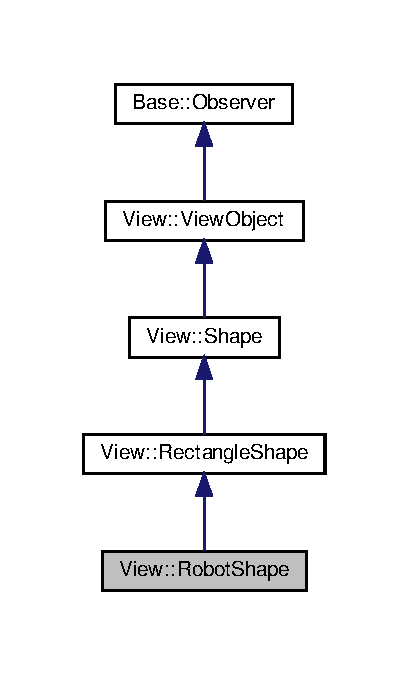
\includegraphics[width=196pt]{class_view_1_1_robot_shape__inherit__graph}
\end{center}
\end{figure}


Collaboration diagram for View\+:\+:Robot\+Shape\+:
\nopagebreak
\begin{figure}[H]
\begin{center}
\leavevmode
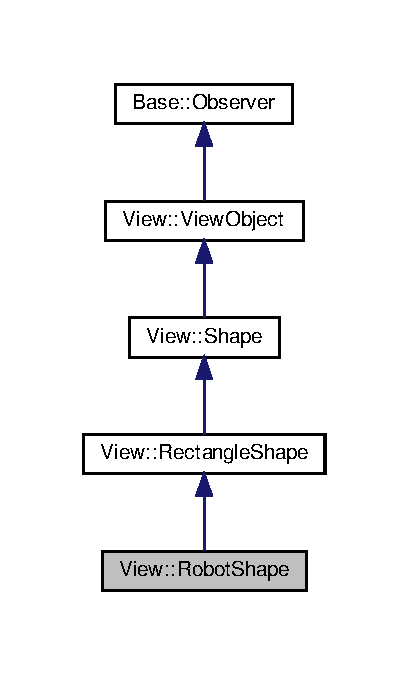
\includegraphics[width=196pt]{class_view_1_1_robot_shape__coll__graph}
\end{center}
\end{figure}
\subsection*{Public Member Functions}
\begin{DoxyCompactItemize}
\item 
{\bfseries Robot\+Shape} (model\+::\+Robot\+Ptr a\+Robot)\hypertarget{class_view_1_1_robot_shape_aec0d01a762c2113a506948b65adea65d}{}\label{class_view_1_1_robot_shape_aec0d01a762c2113a506948b65adea65d}

\item 
virtual std\+::string {\bfseries get\+Normal\+Colour} () const \hypertarget{class_view_1_1_robot_shape_a5a7682a891c8b4bef7304894d2ab2737}{}\label{class_view_1_1_robot_shape_a5a7682a891c8b4bef7304894d2ab2737}

\item 
virtual std\+::string {\bfseries get\+Selection\+Colour} () const \hypertarget{class_view_1_1_robot_shape_a33ac56f82802eb45edaf2fada9635fad}{}\label{class_view_1_1_robot_shape_a33ac56f82802eb45edaf2fada9635fad}

\item 
virtual std\+::string {\bfseries get\+Activation\+Colour} () const \hypertarget{class_view_1_1_robot_shape_a41320fd63ea2f27563c65953d012899a}{}\label{class_view_1_1_robot_shape_a41320fd63ea2f27563c65953d012899a}

\item 
virtual void \hyperlink{class_view_1_1_robot_shape_ab07702949d9d374331a17db4759f0762}{handle\+Activated} ()
\item 
virtual void \hyperlink{class_view_1_1_robot_shape_a8983c43b4ec8cd9eda0f4e32a8f69b19}{handle\+Selection} ()
\item 
void {\bfseries set\+Robot\+World\+Canvas} (\hyperlink{class_view_1_1_robot_world_canvas}{Robot\+World\+Canvas} $\ast$a\+Robot\+World\+Canvas)\hypertarget{class_view_1_1_robot_shape_a95202f41f8b9d066be8625cf6aae0fcb}{}\label{class_view_1_1_robot_shape_a95202f41f8b9d066be8625cf6aae0fcb}

\end{DoxyCompactItemize}
\begin{Indent}{\bf Type safe accessors and mutators}\par
\begin{DoxyCompactItemize}
\item 
model\+::\+Robot\+Ptr \hyperlink{class_view_1_1_robot_shape_a23eca8fea0a58ba16b405b0f0eadf5da}{get\+Robot} () const
\item 
void \hyperlink{class_view_1_1_robot_shape_a96002bd3f90ced18aa3f0ab9b57902a3}{set\+Robot} (model\+::\+Robot\+Ptr a\+Robot)
\end{DoxyCompactItemize}
\end{Indent}
\begin{Indent}{\bf Observer functions}\par
\begin{DoxyCompactItemize}
\item 
virtual void \hyperlink{class_view_1_1_robot_shape_aa8e3a33d23b11a1f9c4580ff46d3d9f7}{handle\+Notification} ()
\end{DoxyCompactItemize}
\end{Indent}
\begin{Indent}{\bf Pure virtual abstract Shape functions}\par
\begin{DoxyCompactItemize}
\item 
virtual void {\bfseries draw} (wx\+DC \&dc)\hypertarget{class_view_1_1_robot_shape_a9f12f9abfa2d4ebfa47b06e02c71d23c}{}\label{class_view_1_1_robot_shape_a9f12f9abfa2d4ebfa47b06e02c71d23c}

\item 
virtual bool \hyperlink{class_view_1_1_robot_shape_aff3acf7b0326d17f5cabdc19c7164095}{occupies} (const Point \&a\+Point) const 
\item 
virtual void {\bfseries set\+Centre} (const Point \&a\+Point)\hypertarget{class_view_1_1_robot_shape_a4b12a96d27b17153069e8864258f52df}{}\label{class_view_1_1_robot_shape_a4b12a96d27b17153069e8864258f52df}

\end{DoxyCompactItemize}
\end{Indent}
\begin{Indent}{\bf Debug functions}\par
\begin{DoxyCompactItemize}
\item 
virtual std\+::string \hyperlink{class_view_1_1_robot_shape_a2af7fa2dfdf390213a921751fb144afa}{as\+String} () const 
\item 
virtual std\+::string \hyperlink{class_view_1_1_robot_shape_afb69a3cb5c895002b054807d26291579}{as\+Debug\+String} () const 
\end{DoxyCompactItemize}
\end{Indent}
\subsection*{Additional Inherited Members}


\subsection{Member Function Documentation}
\index{View\+::\+Robot\+Shape@{View\+::\+Robot\+Shape}!as\+Debug\+String@{as\+Debug\+String}}
\index{as\+Debug\+String@{as\+Debug\+String}!View\+::\+Robot\+Shape@{View\+::\+Robot\+Shape}}
\subsubsection[{\texorpdfstring{as\+Debug\+String() const }{asDebugString() const }}]{\setlength{\rightskip}{0pt plus 5cm}std\+::string View\+::\+Robot\+Shape\+::as\+Debug\+String (
\begin{DoxyParamCaption}
{}
\end{DoxyParamCaption}
) const\hspace{0.3cm}{\ttfamily [virtual]}}\hypertarget{class_view_1_1_robot_shape_afb69a3cb5c895002b054807d26291579}{}\label{class_view_1_1_robot_shape_afb69a3cb5c895002b054807d26291579}
Returns a description of the object with all data of the object usable for debugging 

Reimplemented from \hyperlink{class_view_1_1_rectangle_shape_ae46b92ba72ec4a590afbd106ced79c98}{View\+::\+Rectangle\+Shape}.

\index{View\+::\+Robot\+Shape@{View\+::\+Robot\+Shape}!as\+String@{as\+String}}
\index{as\+String@{as\+String}!View\+::\+Robot\+Shape@{View\+::\+Robot\+Shape}}
\subsubsection[{\texorpdfstring{as\+String() const }{asString() const }}]{\setlength{\rightskip}{0pt plus 5cm}std\+::string View\+::\+Robot\+Shape\+::as\+String (
\begin{DoxyParamCaption}
{}
\end{DoxyParamCaption}
) const\hspace{0.3cm}{\ttfamily [virtual]}}\hypertarget{class_view_1_1_robot_shape_a2af7fa2dfdf390213a921751fb144afa}{}\label{class_view_1_1_robot_shape_a2af7fa2dfdf390213a921751fb144afa}
Returns a 1-\/line description of the object 

Reimplemented from \hyperlink{class_view_1_1_rectangle_shape_a82517a7fb6b1b0331efaa79f306ecc38}{View\+::\+Rectangle\+Shape}.

\index{View\+::\+Robot\+Shape@{View\+::\+Robot\+Shape}!get\+Robot@{get\+Robot}}
\index{get\+Robot@{get\+Robot}!View\+::\+Robot\+Shape@{View\+::\+Robot\+Shape}}
\subsubsection[{\texorpdfstring{get\+Robot() const }{getRobot() const }}]{\setlength{\rightskip}{0pt plus 5cm}model\+::\+Robot\+Ptr View\+::\+Robot\+Shape\+::get\+Robot (
\begin{DoxyParamCaption}
{}
\end{DoxyParamCaption}
) const}\hypertarget{class_view_1_1_robot_shape_a23eca8fea0a58ba16b405b0f0eadf5da}{}\label{class_view_1_1_robot_shape_a23eca8fea0a58ba16b405b0f0eadf5da}
Type safe accessor \index{View\+::\+Robot\+Shape@{View\+::\+Robot\+Shape}!handle\+Activated@{handle\+Activated}}
\index{handle\+Activated@{handle\+Activated}!View\+::\+Robot\+Shape@{View\+::\+Robot\+Shape}}
\subsubsection[{\texorpdfstring{handle\+Activated()}{handleActivated()}}]{\setlength{\rightskip}{0pt plus 5cm}void View\+::\+Robot\+Shape\+::handle\+Activated (
\begin{DoxyParamCaption}
{}
\end{DoxyParamCaption}
)\hspace{0.3cm}{\ttfamily [virtual]}}\hypertarget{class_view_1_1_robot_shape_ab07702949d9d374331a17db4759f0762}{}\label{class_view_1_1_robot_shape_ab07702949d9d374331a17db4759f0762}
This function is called by the \hyperlink{class_view_1_1_robot_world_canvas}{Robot\+World\+Canvas} if enable\+Activation is set. 

Reimplemented from \hyperlink{class_view_1_1_rectangle_shape_a6e075b3fda71d5dd4fbd3f3f9ff42126}{View\+::\+Rectangle\+Shape}.

\index{View\+::\+Robot\+Shape@{View\+::\+Robot\+Shape}!handle\+Notification@{handle\+Notification}}
\index{handle\+Notification@{handle\+Notification}!View\+::\+Robot\+Shape@{View\+::\+Robot\+Shape}}
\subsubsection[{\texorpdfstring{handle\+Notification()}{handleNotification()}}]{\setlength{\rightskip}{0pt plus 5cm}void View\+::\+Robot\+Shape\+::handle\+Notification (
\begin{DoxyParamCaption}
{}
\end{DoxyParamCaption}
)\hspace{0.3cm}{\ttfamily [virtual]}}\hypertarget{class_view_1_1_robot_shape_aa8e3a33d23b11a1f9c4580ff46d3d9f7}{}\label{class_view_1_1_robot_shape_aa8e3a33d23b11a1f9c4580ff46d3d9f7}
A Notifier will call this function if this Observer will handle the notifications of that Notifier. It is the responsibility of the Observer to filter any events it is interested in. 

Reimplemented from \hyperlink{class_view_1_1_rectangle_shape_acae95cb4b05d77196451520ee7d7ca9c}{View\+::\+Rectangle\+Shape}.

\index{View\+::\+Robot\+Shape@{View\+::\+Robot\+Shape}!handle\+Selection@{handle\+Selection}}
\index{handle\+Selection@{handle\+Selection}!View\+::\+Robot\+Shape@{View\+::\+Robot\+Shape}}
\subsubsection[{\texorpdfstring{handle\+Selection()}{handleSelection()}}]{\setlength{\rightskip}{0pt plus 5cm}void View\+::\+Robot\+Shape\+::handle\+Selection (
\begin{DoxyParamCaption}
{}
\end{DoxyParamCaption}
)\hspace{0.3cm}{\ttfamily [virtual]}}\hypertarget{class_view_1_1_robot_shape_a8983c43b4ec8cd9eda0f4e32a8f69b19}{}\label{class_view_1_1_robot_shape_a8983c43b4ec8cd9eda0f4e32a8f69b19}
This function is called by the \hyperlink{class_view_1_1_robot_world_canvas}{Robot\+World\+Canvas} if enable\+Selection is set. 

Reimplemented from \hyperlink{class_view_1_1_rectangle_shape_a15a3cd81166a65e5734b79c87552db00}{View\+::\+Rectangle\+Shape}.

\index{View\+::\+Robot\+Shape@{View\+::\+Robot\+Shape}!occupies@{occupies}}
\index{occupies@{occupies}!View\+::\+Robot\+Shape@{View\+::\+Robot\+Shape}}
\subsubsection[{\texorpdfstring{occupies(const Point \&a\+Point) const }{occupies(const Point &aPoint) const }}]{\setlength{\rightskip}{0pt plus 5cm}bool View\+::\+Robot\+Shape\+::occupies (
\begin{DoxyParamCaption}
\item[{const Point \&}]{a\+Point}
\end{DoxyParamCaption}
) const\hspace{0.3cm}{\ttfamily [virtual]}}\hypertarget{class_view_1_1_robot_shape_aff3acf7b0326d17f5cabdc19c7164095}{}\label{class_view_1_1_robot_shape_aff3acf7b0326d17f5cabdc19c7164095}

\begin{DoxyParams}{Parameters}
{\em a\+Point} & \\
\hline
\end{DoxyParams}
\begin{DoxyReturn}{Returns}
True if the point is in the shape 
\end{DoxyReturn}


Reimplemented from \hyperlink{class_view_1_1_rectangle_shape_ac736dfe69f1a3633696d8c663cd49b51}{View\+::\+Rectangle\+Shape}.

\index{View\+::\+Robot\+Shape@{View\+::\+Robot\+Shape}!set\+Robot@{set\+Robot}}
\index{set\+Robot@{set\+Robot}!View\+::\+Robot\+Shape@{View\+::\+Robot\+Shape}}
\subsubsection[{\texorpdfstring{set\+Robot(\+model\+::\+Robot\+Ptr a\+Robot)}{setRobot(model::RobotPtr aRobot)}}]{\setlength{\rightskip}{0pt plus 5cm}void View\+::\+Robot\+Shape\+::set\+Robot (
\begin{DoxyParamCaption}
\item[{model\+::\+Robot\+Ptr}]{a\+Robot}
\end{DoxyParamCaption}
)}\hypertarget{class_view_1_1_robot_shape_a96002bd3f90ced18aa3f0ab9b57902a3}{}\label{class_view_1_1_robot_shape_a96002bd3f90ced18aa3f0ab9b57902a3}
Type safe mutator 

The documentation for this class was generated from the following files\+:\begin{DoxyCompactItemize}
\item 
/home/hqnders/\+Documents/robotworld/src/Robot\+Shape.\+hpp\item 
/home/hqnders/\+Documents/robotworld/src/Robot\+Shape.\+cpp\end{DoxyCompactItemize}

\hypertarget{class_model_1_1_robot_world}{}\section{model\+:\+:Robot\+World Class Reference}
\label{class_model_1_1_robot_world}\index{model\+::\+Robot\+World@{model\+::\+Robot\+World}}


Inheritance diagram for model\+:\+:Robot\+World\+:
\nopagebreak
\begin{figure}[H]
\begin{center}
\leavevmode
\includegraphics[width=350pt]{class_model_1_1_robot_world__inherit__graph}
\end{center}
\end{figure}


Collaboration diagram for model\+:\+:Robot\+World\+:
\nopagebreak
\begin{figure}[H]
\begin{center}
\leavevmode
\includegraphics[width=350pt]{class_model_1_1_robot_world__coll__graph}
\end{center}
\end{figure}
\subsection*{Public Member Functions}
\begin{DoxyCompactItemize}
\item 
Robot\+Ptr {\bfseries new\+Robot} (const std\+::string \&a\+Name=\char`\"{}New \hyperlink{class_model_1_1_robot}{Robot}\char`\"{}, const Point \&a\+Position=Point(-\/1,-\/1), bool a\+Notify\+Observers=true)\hypertarget{class_model_1_1_robot_world_af0d58001395b3b375c2a98b28f2f3ef2}{}\label{class_model_1_1_robot_world_af0d58001395b3b375c2a98b28f2f3ef2}

\item 
Way\+Point\+Ptr {\bfseries new\+Way\+Point} (const std\+::string \&a\+Name=\char`\"{}New \hyperlink{class_model_1_1_way_point}{Way\+Point}\char`\"{}, const Point \&a\+Position=Point(-\/1,-\/1), bool a\+Notify\+Observers=true)\hypertarget{class_model_1_1_robot_world_a45272003383e53e4d8273e83a3e7dc7f}{}\label{class_model_1_1_robot_world_a45272003383e53e4d8273e83a3e7dc7f}

\item 
Goal\+Ptr {\bfseries new\+Goal} (const std\+::string \&a\+Name=\char`\"{}New \hyperlink{class_model_1_1_goal}{Goal}\char`\"{}, const Point \&a\+Position=Point(-\/1,-\/1), bool a\+Notify\+Observers=true)\hypertarget{class_model_1_1_robot_world_afc21f82cc1c2c65655da7ef6a7e0f6e5}{}\label{class_model_1_1_robot_world_afc21f82cc1c2c65655da7ef6a7e0f6e5}

\item 
Wall\+Ptr {\bfseries new\+Wall} (const Point \&a\+Point1, const Point \&a\+Point2, bool a\+Notify\+Observers=true)\hypertarget{class_model_1_1_robot_world_a8b3d9243b9550a6fe01bc3b880fadec5}{}\label{class_model_1_1_robot_world_a8b3d9243b9550a6fe01bc3b880fadec5}

\item 
void {\bfseries delete\+Robot} (Robot\+Ptr a\+Robot, bool a\+Notify\+Observers=true)\hypertarget{class_model_1_1_robot_world_aa6d7a030f609d6b1187b1c5e93469695}{}\label{class_model_1_1_robot_world_aa6d7a030f609d6b1187b1c5e93469695}

\item 
void {\bfseries delete\+Way\+Point} (Way\+Point\+Ptr a\+Way\+Point, bool a\+Notify\+Observers=true)\hypertarget{class_model_1_1_robot_world_afbb97c93d8d68e6e624af6fc988b57ca}{}\label{class_model_1_1_robot_world_afbb97c93d8d68e6e624af6fc988b57ca}

\item 
void {\bfseries delete\+Goal} (Goal\+Ptr a\+Goal, bool a\+Notify\+Observers=true)\hypertarget{class_model_1_1_robot_world_a5208d73a57a8b663f4de407150fb8379}{}\label{class_model_1_1_robot_world_a5208d73a57a8b663f4de407150fb8379}

\item 
void {\bfseries delete\+Wall} (Wall\+Ptr a\+Wall, bool a\+Notify\+Observers=true)\hypertarget{class_model_1_1_robot_world_a25c789a5165ee686ef21e1492aace738}{}\label{class_model_1_1_robot_world_a25c789a5165ee686ef21e1492aace738}

\item 
Robot\+Ptr {\bfseries get\+Robot} (const std\+::string \&a\+Name) const \hypertarget{class_model_1_1_robot_world_aa65fc818fe12a23953ac53f7f62705fb}{}\label{class_model_1_1_robot_world_aa65fc818fe12a23953ac53f7f62705fb}

\item 
Robot\+Ptr {\bfseries get\+Robot} (const \hyperlink{class_base_1_1_object_id}{Base\+::\+Object\+Id} \&an\+Object\+Id) const \hypertarget{class_model_1_1_robot_world_ac7897e5aa501752e5e93b555efbf752a}{}\label{class_model_1_1_robot_world_ac7897e5aa501752e5e93b555efbf752a}

\item 
Way\+Point\+Ptr {\bfseries get\+Way\+Point} (const std\+::string \&a\+Name) const \hypertarget{class_model_1_1_robot_world_a4ec5350ad359e9b37bd2f5606a86fea1}{}\label{class_model_1_1_robot_world_a4ec5350ad359e9b37bd2f5606a86fea1}

\item 
Way\+Point\+Ptr {\bfseries get\+Way\+Point} (const \hyperlink{class_base_1_1_object_id}{Base\+::\+Object\+Id} \&an\+Object\+Id) const \hypertarget{class_model_1_1_robot_world_a6ce03ec6f6f106172053cdd789844347}{}\label{class_model_1_1_robot_world_a6ce03ec6f6f106172053cdd789844347}

\item 
Goal\+Ptr {\bfseries get\+Goal} (const std\+::string \&a\+Name) const \hypertarget{class_model_1_1_robot_world_aae1b5a0410c5ae207cd8b7525e204cc0}{}\label{class_model_1_1_robot_world_aae1b5a0410c5ae207cd8b7525e204cc0}

\item 
Goal\+Ptr {\bfseries get\+Goal} (const \hyperlink{class_base_1_1_object_id}{Base\+::\+Object\+Id} \&an\+Object\+Id) const \hypertarget{class_model_1_1_robot_world_a3a678aa437a062c21acccf9ed105a3ec}{}\label{class_model_1_1_robot_world_a3a678aa437a062c21acccf9ed105a3ec}

\item 
Wall\+Ptr {\bfseries get\+Wall} (const \hyperlink{class_base_1_1_object_id}{Base\+::\+Object\+Id} \&an\+Object\+Id) const \hypertarget{class_model_1_1_robot_world_a8d6dab46a8c89a42f101f4548e4b3da6}{}\label{class_model_1_1_robot_world_a8d6dab46a8c89a42f101f4548e4b3da6}

\item 
const std\+::vector$<$ Robot\+Ptr $>$ \& {\bfseries get\+Robots} () const \hypertarget{class_model_1_1_robot_world_a657cbe460deb2057521ae51dc5327fe7}{}\label{class_model_1_1_robot_world_a657cbe460deb2057521ae51dc5327fe7}

\item 
const std\+::vector$<$ Way\+Point\+Ptr $>$ \& {\bfseries get\+Way\+Points} () const \hypertarget{class_model_1_1_robot_world_a1bbc183d9e63ae142bcbc0373aa06e78}{}\label{class_model_1_1_robot_world_a1bbc183d9e63ae142bcbc0373aa06e78}

\item 
const std\+::vector$<$ Goal\+Ptr $>$ \& {\bfseries get\+Goals} () const \hypertarget{class_model_1_1_robot_world_a6bac601255c803cc88cc145da2aa1ff0}{}\label{class_model_1_1_robot_world_a6bac601255c803cc88cc145da2aa1ff0}

\item 
const std\+::vector$<$ Wall\+Ptr $>$ \& {\bfseries get\+Walls} () const \hypertarget{class_model_1_1_robot_world_a6751f9fe7b9e33047a6d518f5a2f819b}{}\label{class_model_1_1_robot_world_a6751f9fe7b9e33047a6d518f5a2f819b}

\item 
void {\bfseries populate} (int a\+Number\+Of\+Walls=2)\hypertarget{class_model_1_1_robot_world_afe09ff15bf8a4cbed1222baa065107d9}{}\label{class_model_1_1_robot_world_afe09ff15bf8a4cbed1222baa065107d9}

\item 
void {\bfseries unpopulate} (bool a\+Notify\+Observers=true)\hypertarget{class_model_1_1_robot_world_aa54ca5337df73d34be09a2c3b9a66c37}{}\label{class_model_1_1_robot_world_aa54ca5337df73d34be09a2c3b9a66c37}

\item 
void \hyperlink{class_model_1_1_robot_world_a4a62b951e0cdab0ce60f0189442481f8}{unpopulate} (const std\+::vector$<$ \hyperlink{class_base_1_1_object_id}{Base\+::\+Object\+Id} $>$ \&a\+Keep\+Objects, bool a\+Notify\+Observers=true)
\end{DoxyCompactItemize}
\begin{Indent}{\bf Debug functions}\par
\begin{DoxyCompactItemize}
\item 
virtual std\+::string \hyperlink{class_model_1_1_robot_world_a9f5a599b9d6523f45df7cbb0aafe4c08}{as\+String} () const 
\item 
virtual std\+::string \hyperlink{class_model_1_1_robot_world_a9c599037d4bdc7ebd4e9138c3cf3cc82}{as\+Debug\+String} () const 
\end{DoxyCompactItemize}
\end{Indent}
\subsection*{Static Public Member Functions}
\begin{DoxyCompactItemize}
\item 
static \hyperlink{class_model_1_1_robot_world}{Robot\+World} \& {\bfseries get\+Robot\+World} ()\hypertarget{class_model_1_1_robot_world_a3129fe115ffa78851d1d81e62a87bfa0}{}\label{class_model_1_1_robot_world_a3129fe115ffa78851d1d81e62a87bfa0}

\end{DoxyCompactItemize}


\subsection{Member Function Documentation}
\index{model\+::\+Robot\+World@{model\+::\+Robot\+World}!as\+Debug\+String@{as\+Debug\+String}}
\index{as\+Debug\+String@{as\+Debug\+String}!model\+::\+Robot\+World@{model\+::\+Robot\+World}}
\subsubsection[{\texorpdfstring{as\+Debug\+String() const }{asDebugString() const }}]{\setlength{\rightskip}{0pt plus 5cm}std\+::string model\+::\+Robot\+World\+::as\+Debug\+String (
\begin{DoxyParamCaption}
{}
\end{DoxyParamCaption}
) const\hspace{0.3cm}{\ttfamily [virtual]}}\hypertarget{class_model_1_1_robot_world_a9c599037d4bdc7ebd4e9138c3cf3cc82}{}\label{class_model_1_1_robot_world_a9c599037d4bdc7ebd4e9138c3cf3cc82}
Returns a description of the object with all data of the object usable for debugging 

Reimplemented from \hyperlink{class_model_1_1_model_object_aced22b0b0ee637c598c463de6a1d8d03}{model\+::\+model\+Object}.

\index{model\+::\+Robot\+World@{model\+::\+Robot\+World}!as\+String@{as\+String}}
\index{as\+String@{as\+String}!model\+::\+Robot\+World@{model\+::\+Robot\+World}}
\subsubsection[{\texorpdfstring{as\+String() const }{asString() const }}]{\setlength{\rightskip}{0pt plus 5cm}std\+::string model\+::\+Robot\+World\+::as\+String (
\begin{DoxyParamCaption}
{}
\end{DoxyParamCaption}
) const\hspace{0.3cm}{\ttfamily [virtual]}}\hypertarget{class_model_1_1_robot_world_a9f5a599b9d6523f45df7cbb0aafe4c08}{}\label{class_model_1_1_robot_world_a9f5a599b9d6523f45df7cbb0aafe4c08}
Returns a 1-\/line description of the object 

Reimplemented from \hyperlink{class_model_1_1_model_object_a9db00b9150a932a1637e425f24c0bdf0}{model\+::\+model\+Object}.

\index{model\+::\+Robot\+World@{model\+::\+Robot\+World}!unpopulate@{unpopulate}}
\index{unpopulate@{unpopulate}!model\+::\+Robot\+World@{model\+::\+Robot\+World}}
\subsubsection[{\texorpdfstring{unpopulate(const std\+::vector$<$ Base\+::\+Object\+Id $>$ \&a\+Keep\+Objects, bool a\+Notify\+Observers=true)}{unpopulate(const std::vector< Base::ObjectId > &aKeepObjects, bool aNotifyObservers=true)}}]{\setlength{\rightskip}{0pt plus 5cm}void model\+::\+Robot\+World\+::unpopulate (
\begin{DoxyParamCaption}
\item[{const std\+::vector$<$ {\bf Base\+::\+Object\+Id} $>$ \&}]{a\+Keep\+Objects, }
\item[{bool}]{a\+Notify\+Observers = {\ttfamily true}}
\end{DoxyParamCaption}
)}\hypertarget{class_model_1_1_robot_world_a4a62b951e0cdab0ce60f0189442481f8}{}\label{class_model_1_1_robot_world_a4a62b951e0cdab0ce60f0189442481f8}

\begin{DoxyParams}{Parameters}
{\em a\+Keep\+Objects} & Keep the objects with these Object\+Idsin the world \\
\hline
{\em a\+Notify\+Observers} & \\
\hline
\end{DoxyParams}


The documentation for this class was generated from the following files\+:\begin{DoxyCompactItemize}
\item 
/home/hqnders/\+Documents/robotworld/src/Robot\+World.\+hpp\item 
/home/hqnders/\+Documents/robotworld/src/Robot\+World.\+cpp\end{DoxyCompactItemize}

\hypertarget{class_view_1_1_robot_world_canvas}{}\section{View\+:\+:Robot\+World\+Canvas Class Reference}
\label{class_view_1_1_robot_world_canvas}\index{View\+::\+Robot\+World\+Canvas@{View\+::\+Robot\+World\+Canvas}}


Inheritance diagram for View\+:\+:Robot\+World\+Canvas\+:
\nopagebreak
\begin{figure}[H]
\begin{center}
\leavevmode
\includegraphics[width=280pt]{class_view_1_1_robot_world_canvas__inherit__graph}
\end{center}
\end{figure}


Collaboration diagram for View\+:\+:Robot\+World\+Canvas\+:
\nopagebreak
\begin{figure}[H]
\begin{center}
\leavevmode
\includegraphics[width=280pt]{class_view_1_1_robot_world_canvas__coll__graph}
\end{center}
\end{figure}
\subsection*{Public Member Functions}
\begin{DoxyCompactItemize}
\item 
{\bfseries Robot\+World\+Canvas} (Window $\ast$an\+Owner)\hypertarget{class_view_1_1_robot_world_canvas_afc6ffd527bcd9970f12e5fd70a841782}{}\label{class_view_1_1_robot_world_canvas_afc6ffd527bcd9970f12e5fd70a841782}

\item 
{\bfseries Robot\+World\+Canvas} (Window $\ast$an\+Owner, model\+::\+model\+Object\+Ptr a\+model\+Object)\hypertarget{class_view_1_1_robot_world_canvas_aff3e613f2782874b4560a015be7b6180}{}\label{class_view_1_1_robot_world_canvas_aff3e613f2782874b4560a015be7b6180}

\item 
Point \hyperlink{class_view_1_1_robot_world_canvas_a7cffeb2971aaac6039398b6d896fd3b1}{device\+Point\+For} (const Point \&a\+Screen\+Point) const 
\item 
Point \hyperlink{class_view_1_1_robot_world_canvas_a0f505fef4f08daaa9ebd21ff392c698f}{screen\+Point\+For} (const Point \&a\+Device\+Point) const 
\item 
bool \hyperlink{class_view_1_1_robot_world_canvas_ac4fefdf43774d0f90c469527b1d27fd3}{is\+Shape\+Selected} () const 
\item 
virtual Shape\+Ptr \hyperlink{class_view_1_1_robot_world_canvas_aefd5c6dc27fe807047996443797594a0}{get\+Selected\+Shape} () const 
\item 
virtual void \hyperlink{class_view_1_1_robot_world_canvas_a51477f3840089817d00ed6f2dee7c69e}{set\+Selected\+Shape} (Shape\+Ptr a\+Selected\+Shape)
\item 
virtual bool \hyperlink{class_view_1_1_robot_world_canvas_a38bc5c3dd6eb99504fc1ada58ed39a14}{is\+Shape\+At} (const Point \&a\+Point) const 
\item 
virtual Shape\+Ptr \hyperlink{class_view_1_1_robot_world_canvas_a625bdb271e6426cc7c228c4c71eebedf}{get\+Shape\+At} (const Point \&a\+Point) const 
\item 
virtual bool \hyperlink{class_view_1_1_robot_world_canvas_a91fc7b9d37d228ba9285fe82dab04fbb}{select\+Shape\+At} (const Point \&a\+Point)
\item 
virtual void \hyperlink{class_view_1_1_robot_world_canvas_a19aa6f46000f7f7db267f6aec911f25f}{handle\+Back\+Ground\+Notification} ()
\item 
void \hyperlink{class_view_1_1_robot_world_canvas_ab498b81c0619bc6109548582addc7e02}{populate} (int a\+Number\+Of\+Walls=2)
\item 
void \hyperlink{class_view_1_1_robot_world_canvas_a20eb2ae3ba32d1a1b8994025e0c6bc39}{unpopulate} ()
\end{DoxyCompactItemize}
\begin{Indent}{\bf Event handling enabling functions}\par
\begin{DoxyCompactItemize}
\item 
virtual void {\bfseries enable\+Handle\+Paint} (bool enable=true)\hypertarget{class_view_1_1_robot_world_canvas_ac74704c6f3337c017a338aa60ac550a6}{}\label{class_view_1_1_robot_world_canvas_ac74704c6f3337c017a338aa60ac550a6}

\item 
virtual void {\bfseries enable\+Handle\+Size} (bool enable=true)\hypertarget{class_view_1_1_robot_world_canvas_a9a85f803ceea25f82b6dab3a68b51915}{}\label{class_view_1_1_robot_world_canvas_a9a85f803ceea25f82b6dab3a68b51915}

\item 
virtual void {\bfseries enable\+Left\+Down\+Handling} (bool enable=true)\hypertarget{class_view_1_1_robot_world_canvas_aff53f317176e354f858710ad334473b1}{}\label{class_view_1_1_robot_world_canvas_aff53f317176e354f858710ad334473b1}

\item 
virtual void {\bfseries enable\+Left\+Up\+Handling} (bool enable=true)\hypertarget{class_view_1_1_robot_world_canvas_adae323b06595ebe6c203beedd1f88594}{}\label{class_view_1_1_robot_world_canvas_adae323b06595ebe6c203beedd1f88594}

\item 
virtual void {\bfseries enable\+Left\+D\+Click\+Handling} (bool enable=true)\hypertarget{class_view_1_1_robot_world_canvas_ad34bec03c60bc74967da0815bfc3decb}{}\label{class_view_1_1_robot_world_canvas_ad34bec03c60bc74967da0815bfc3decb}

\item 
virtual void {\bfseries enable\+Middle\+Down\+Handling} (bool enable=true)\hypertarget{class_view_1_1_robot_world_canvas_a2cf15bd7f032378476292e4ef4baeb60}{}\label{class_view_1_1_robot_world_canvas_a2cf15bd7f032378476292e4ef4baeb60}

\item 
virtual void {\bfseries enable\+Middle\+Up\+Handling} (bool enable=true)\hypertarget{class_view_1_1_robot_world_canvas_aff0f17e087d0c16b61fc3fa4664d9280}{}\label{class_view_1_1_robot_world_canvas_aff0f17e087d0c16b61fc3fa4664d9280}

\item 
virtual void {\bfseries enable\+Middle\+D\+Click\+Handling} (bool enable=true)\hypertarget{class_view_1_1_robot_world_canvas_abbf14eaa663020a5c28ddc34b04a7d93}{}\label{class_view_1_1_robot_world_canvas_abbf14eaa663020a5c28ddc34b04a7d93}

\item 
virtual void {\bfseries enable\+Right\+Down\+Handling} (bool enable=true)\hypertarget{class_view_1_1_robot_world_canvas_a8b249411be7ea966eb7ad01698d30ff4}{}\label{class_view_1_1_robot_world_canvas_a8b249411be7ea966eb7ad01698d30ff4}

\item 
virtual void {\bfseries enable\+Right\+Up\+Handling} (bool enable=true)\hypertarget{class_view_1_1_robot_world_canvas_ade500a4e9585a02b05f3c2bdcca59b39}{}\label{class_view_1_1_robot_world_canvas_ade500a4e9585a02b05f3c2bdcca59b39}

\item 
virtual void {\bfseries enable\+Right\+D\+Click\+Handling} (bool enable=true)\hypertarget{class_view_1_1_robot_world_canvas_addbc170d9d9c998af49ffca65ed6216a}{}\label{class_view_1_1_robot_world_canvas_addbc170d9d9c998af49ffca65ed6216a}

\item 
virtual void {\bfseries enable\+Mouse\+Motion\+Handling} (bool enable=true)\hypertarget{class_view_1_1_robot_world_canvas_a6decd9bcd3acac80852476fc30f5df8e}{}\label{class_view_1_1_robot_world_canvas_a6decd9bcd3acac80852476fc30f5df8e}

\item 
virtual void {\bfseries enable\+Key\+Handling} (bool enable=true)\hypertarget{class_view_1_1_robot_world_canvas_a531ca3c86af833a551ad9f3606cd4c9f}{}\label{class_view_1_1_robot_world_canvas_a531ca3c86af833a551ad9f3606cd4c9f}

\item 
virtual void {\bfseries enable\+Activation\+Handling} (bool enable=true)\hypertarget{class_view_1_1_robot_world_canvas_a652f1eec754019d4d8e3c32a7749545f}{}\label{class_view_1_1_robot_world_canvas_a652f1eec754019d4d8e3c32a7749545f}

\item 
virtual void {\bfseries enable\+Selection\+Handling} (bool enable=true)\hypertarget{class_view_1_1_robot_world_canvas_a6e0de11c21b2b482c440cc3b1dfc70ca}{}\label{class_view_1_1_robot_world_canvas_a6e0de11c21b2b482c440cc3b1dfc70ca}

\item 
virtual void {\bfseries enable\+Item\+Menu\+Handling} (bool enable=true)\hypertarget{class_view_1_1_robot_world_canvas_ad030befe82d71f44547da7c180427367}{}\label{class_view_1_1_robot_world_canvas_ad030befe82d71f44547da7c180427367}

\item 
virtual void {\bfseries enable\+Drag\+And\+Drop\+Handling} (bool enable=true)\hypertarget{class_view_1_1_robot_world_canvas_a923d937443987722653140d1f22e16b9}{}\label{class_view_1_1_robot_world_canvas_a923d937443987722653140d1f22e16b9}

\end{DoxyCompactItemize}
\end{Indent}
\begin{Indent}{\bf Type safe accessors and mutators}\par
\begin{DoxyCompactItemize}
\item 
model\+::\+Robot\+World\+Ptr \hyperlink{class_view_1_1_robot_world_canvas_ae82885a5dd5ce493c8b3df3a7d0385a4}{get\+Robot\+World} () const
\item 
void \hyperlink{class_view_1_1_robot_world_canvas_a2829529a8b4221f072aeac196bbc9b17}{set\+Robot\+World} (model\+::\+Robot\+World\+Ptr a\+Robot\+World)
\end{DoxyCompactItemize}
\end{Indent}
\begin{Indent}{\bf Observer functions}\par
\begin{DoxyCompactItemize}
\item 
virtual void \hyperlink{class_view_1_1_robot_world_canvas_af24f07e5484dbba2edd563c826694098}{handle\+Notification} ()
\end{DoxyCompactItemize}
\end{Indent}
\subsection*{Protected Member Functions}
\begin{DoxyCompactItemize}
\item 
void \hyperlink{class_view_1_1_robot_world_canvas_a976c8eb03167bf9c9b0f911ff3e0fa9e}{initialise} ()
\item 
void {\bfseries render} (wx\+DC \&dc)\hypertarget{class_view_1_1_robot_world_canvas_a9cc3e904305ee1e99f916ecdcbd757b7}{}\label{class_view_1_1_robot_world_canvas_a9cc3e904305ee1e99f916ecdcbd757b7}

\item 
virtual void {\bfseries handle\+Activation} (Shape\+Ptr a\+Shape)\hypertarget{class_view_1_1_robot_world_canvas_a29d4e61d22b79fedaee17411b5f6b3c7}{}\label{class_view_1_1_robot_world_canvas_a29d4e61d22b79fedaee17411b5f6b3c7}

\item 
virtual void {\bfseries handle\+Selection} (Shape\+Ptr a\+Shape)\hypertarget{class_view_1_1_robot_world_canvas_a955374b23557c1459b597e457d68cf57}{}\label{class_view_1_1_robot_world_canvas_a955374b23557c1459b597e457d68cf57}

\item 
virtual void {\bfseries handle\+Menu} (const Point \&a\+Screen\+Point)\hypertarget{class_view_1_1_robot_world_canvas_a11ae3a4bc7c60fb560d42c1f63b8955b}{}\label{class_view_1_1_robot_world_canvas_a11ae3a4bc7c60fb560d42c1f63b8955b}

\item 
virtual void {\bfseries handle\+Item\+Menu} (Shape\+Ptr a\+Selected\+Shape, const Point \&a\+Point)\hypertarget{class_view_1_1_robot_world_canvas_a29edcdeeea1b21b5626b1f47fbe43871}{}\label{class_view_1_1_robot_world_canvas_a29edcdeeea1b21b5626b1f47fbe43871}

\item 
void {\bfseries add\+Shape} (Robot\+Shape\+Ptr a\+Robot\+Shape)\hypertarget{class_view_1_1_robot_world_canvas_a3156a2e906d30e96f9bf7ef9ff731b06}{}\label{class_view_1_1_robot_world_canvas_a3156a2e906d30e96f9bf7ef9ff731b06}

\item 
void {\bfseries add\+Shape} (Goal\+Shape\+Ptr a\+Goal\+Shape)\hypertarget{class_view_1_1_robot_world_canvas_afaa1fc0f2e6e76653ef7022853318646}{}\label{class_view_1_1_robot_world_canvas_afaa1fc0f2e6e76653ef7022853318646}

\item 
void {\bfseries add\+Shape} (Way\+Point\+Shape\+Ptr a\+Way\+Point\+Shape)\hypertarget{class_view_1_1_robot_world_canvas_abb5dee13a6e25baf0980129cfb1780d3}{}\label{class_view_1_1_robot_world_canvas_abb5dee13a6e25baf0980129cfb1780d3}

\item 
void {\bfseries add\+Shape} (Wall\+Shape\+Ptr a\+Wall\+Shape)\hypertarget{class_view_1_1_robot_world_canvas_a51c5fac3c75b4ebc258511bf00c93863}{}\label{class_view_1_1_robot_world_canvas_a51c5fac3c75b4ebc258511bf00c93863}

\item 
void {\bfseries remove\+Shape} (Robot\+Shape\+Ptr a\+Robot\+Shape)\hypertarget{class_view_1_1_robot_world_canvas_ac40c2e62c75618d63e09a0d4f0ca4bb4}{}\label{class_view_1_1_robot_world_canvas_ac40c2e62c75618d63e09a0d4f0ca4bb4}

\item 
void {\bfseries remove\+Shape} (Goal\+Shape\+Ptr a\+Goal\+Shape)\hypertarget{class_view_1_1_robot_world_canvas_a274b8ff8d7d6bfe6e40c04cbd1c526de}{}\label{class_view_1_1_robot_world_canvas_a274b8ff8d7d6bfe6e40c04cbd1c526de}

\item 
void {\bfseries remove\+Shape} (Way\+Point\+Shape\+Ptr a\+Way\+Point\+Shape)\hypertarget{class_view_1_1_robot_world_canvas_ae94d4410e1250dfc2c2221265be10c24}{}\label{class_view_1_1_robot_world_canvas_ae94d4410e1250dfc2c2221265be10c24}

\item 
void {\bfseries remove\+Shape} (Wall\+Shape\+Ptr a\+Wall\+Shape)\hypertarget{class_view_1_1_robot_world_canvas_a14bd783613cbd6aa65eaabfe873d7369}{}\label{class_view_1_1_robot_world_canvas_a14bd783613cbd6aa65eaabfe873d7369}

\item 
void {\bfseries remove\+Generic\+Shape} (Shape\+Ptr a\+Shape)\hypertarget{class_view_1_1_robot_world_canvas_af3ba30c00eaedf7bbb67b731f12d1af7}{}\label{class_view_1_1_robot_world_canvas_af3ba30c00eaedf7bbb67b731f12d1af7}

\end{DoxyCompactItemize}
\begin{Indent}{\bf Event handling functions}\par
{\em Override these functions if the default handling is not what you want }\begin{DoxyCompactItemize}
\item 
virtual void {\bfseries handle\+Paint} (Paint\+Event \&event)\hypertarget{class_view_1_1_robot_world_canvas_a77d292863075ab2e7a51148c86e794b5}{}\label{class_view_1_1_robot_world_canvas_a77d292863075ab2e7a51148c86e794b5}

\item 
virtual void {\bfseries handle\+Size} (Size\+Event \&event)\hypertarget{class_view_1_1_robot_world_canvas_a9e87fc8cfc5d45de10c5b44bdcf32974}{}\label{class_view_1_1_robot_world_canvas_a9e87fc8cfc5d45de10c5b44bdcf32974}

\item 
virtual void {\bfseries handle\+Left\+Down} (Mouse\+Event \&event)\hypertarget{class_view_1_1_robot_world_canvas_a6f01a640b1d11b8a5c399ec1beb5d9dd}{}\label{class_view_1_1_robot_world_canvas_a6f01a640b1d11b8a5c399ec1beb5d9dd}

\item 
virtual void {\bfseries handle\+Left\+Up} (Mouse\+Event \&event)\hypertarget{class_view_1_1_robot_world_canvas_a652bd5372da5fd21ecc2379faf7d5c62}{}\label{class_view_1_1_robot_world_canvas_a652bd5372da5fd21ecc2379faf7d5c62}

\item 
virtual void {\bfseries handle\+Left\+D\+Click} (Mouse\+Event \&event)\hypertarget{class_view_1_1_robot_world_canvas_a6287e395342c737724bebbeb56de826d}{}\label{class_view_1_1_robot_world_canvas_a6287e395342c737724bebbeb56de826d}

\item 
virtual void {\bfseries handle\+Middle\+Down} (Mouse\+Event \&event)\hypertarget{class_view_1_1_robot_world_canvas_af4e64974c6b76b7fa3107694d2a895b8}{}\label{class_view_1_1_robot_world_canvas_af4e64974c6b76b7fa3107694d2a895b8}

\item 
virtual void {\bfseries handle\+Middle\+Up} (Mouse\+Event \&event)\hypertarget{class_view_1_1_robot_world_canvas_a23f3eb4db9fd3b72872f3f8e74425816}{}\label{class_view_1_1_robot_world_canvas_a23f3eb4db9fd3b72872f3f8e74425816}

\item 
virtual void {\bfseries handle\+Middle\+D\+Click} (Mouse\+Event \&event)\hypertarget{class_view_1_1_robot_world_canvas_a1509cf3de672c05fac25b9a63dbd719a}{}\label{class_view_1_1_robot_world_canvas_a1509cf3de672c05fac25b9a63dbd719a}

\item 
virtual void {\bfseries handle\+Right\+Down} (Mouse\+Event \&event)\hypertarget{class_view_1_1_robot_world_canvas_aa0063e9b90265e676d0069dbe6e392ac}{}\label{class_view_1_1_robot_world_canvas_aa0063e9b90265e676d0069dbe6e392ac}

\item 
virtual void {\bfseries handle\+Right\+Up} (Mouse\+Event \&event)\hypertarget{class_view_1_1_robot_world_canvas_a18873d7781c08653b14c9d3a9a0a8346}{}\label{class_view_1_1_robot_world_canvas_a18873d7781c08653b14c9d3a9a0a8346}

\item 
virtual void {\bfseries handle\+Right\+D\+Click} (Mouse\+Event \&event)\hypertarget{class_view_1_1_robot_world_canvas_a97c26bc9722ced6706681077b68dcd20}{}\label{class_view_1_1_robot_world_canvas_a97c26bc9722ced6706681077b68dcd20}

\item 
virtual void {\bfseries handle\+Mouse\+Motion} (Mouse\+Event \&event)\hypertarget{class_view_1_1_robot_world_canvas_af636158a32890d6f44b5e93c4e8bf760}{}\label{class_view_1_1_robot_world_canvas_af636158a32890d6f44b5e93c4e8bf760}

\item 
virtual void {\bfseries handle\+Key} (Key\+Event \&event)\hypertarget{class_view_1_1_robot_world_canvas_ad9b2185e171a240bd9bf54266526d2bc}{}\label{class_view_1_1_robot_world_canvas_ad9b2185e171a240bd9bf54266526d2bc}

\item 
virtual void {\bfseries handle\+Begin\+Left\+Drag} (Shape\+Ptr a\+Shape)\hypertarget{class_view_1_1_robot_world_canvas_a4724659516bdc8572f585073009f5c40}{}\label{class_view_1_1_robot_world_canvas_a4724659516bdc8572f585073009f5c40}

\item 
virtual void {\bfseries handle\+End\+Drag} (Shape\+Ptr a\+Shape)\hypertarget{class_view_1_1_robot_world_canvas_aee572b2a63b6a8b1577ee7b69bf90b87}{}\label{class_view_1_1_robot_world_canvas_aee572b2a63b6a8b1577ee7b69bf90b87}

\item 
virtual void {\bfseries handle\+Add\+Robot} (Command\+Event \&event)\hypertarget{class_view_1_1_robot_world_canvas_abd7db9facf18e6cadd54c2f681df7c66}{}\label{class_view_1_1_robot_world_canvas_abd7db9facf18e6cadd54c2f681df7c66}

\item 
virtual void {\bfseries handle\+Edit\+Robot} (Command\+Event \&event)\hypertarget{class_view_1_1_robot_world_canvas_a57692f00a4e5fb281fc7baf1920f6430}{}\label{class_view_1_1_robot_world_canvas_a57692f00a4e5fb281fc7baf1920f6430}

\item 
virtual void {\bfseries handle\+Delete\+Robot} (Command\+Event \&event)\hypertarget{class_view_1_1_robot_world_canvas_a0d1aeab78b87c7ac297fa877d63d4509}{}\label{class_view_1_1_robot_world_canvas_a0d1aeab78b87c7ac297fa877d63d4509}

\item 
virtual void {\bfseries handle\+Add\+Way\+Point} (Command\+Event \&event)\hypertarget{class_view_1_1_robot_world_canvas_a27d9c2435d11a4a25ba545b2dedb7942}{}\label{class_view_1_1_robot_world_canvas_a27d9c2435d11a4a25ba545b2dedb7942}

\item 
virtual void {\bfseries handle\+Edit\+Way\+Point} (Command\+Event \&event)\hypertarget{class_view_1_1_robot_world_canvas_a28b10cb19c0c0810c329f8730dd26da3}{}\label{class_view_1_1_robot_world_canvas_a28b10cb19c0c0810c329f8730dd26da3}

\item 
virtual void {\bfseries handle\+Delete\+Way\+Point} (Command\+Event \&event)\hypertarget{class_view_1_1_robot_world_canvas_a59a9e54e21bd5bd93bf67b8ea53776c0}{}\label{class_view_1_1_robot_world_canvas_a59a9e54e21bd5bd93bf67b8ea53776c0}

\item 
virtual void {\bfseries handle\+Add\+Goal} (Command\+Event \&event)\hypertarget{class_view_1_1_robot_world_canvas_aec6ff89595e1a7acc7d52617e7382a9d}{}\label{class_view_1_1_robot_world_canvas_aec6ff89595e1a7acc7d52617e7382a9d}

\item 
virtual void {\bfseries handle\+Edit\+Goal} (Command\+Event \&event)\hypertarget{class_view_1_1_robot_world_canvas_a02faf3e677c578a817e6c3e071c40fbd}{}\label{class_view_1_1_robot_world_canvas_a02faf3e677c578a817e6c3e071c40fbd}

\item 
virtual void {\bfseries handle\+Delete\+Goal} (Command\+Event \&event)\hypertarget{class_view_1_1_robot_world_canvas_a373e72f2cda977a78ef7c9dae4fea0e5}{}\label{class_view_1_1_robot_world_canvas_a373e72f2cda977a78ef7c9dae4fea0e5}

\item 
virtual void {\bfseries handle\+Add\+Wall} (Command\+Event \&event)\hypertarget{class_view_1_1_robot_world_canvas_aa95a5735508bdba10ee833be5b9d2052}{}\label{class_view_1_1_robot_world_canvas_aa95a5735508bdba10ee833be5b9d2052}

\item 
virtual void {\bfseries handle\+Edit\+Wall} (Command\+Event \&event)\hypertarget{class_view_1_1_robot_world_canvas_a6c69668363176d9e81579fef5e30ba9e}{}\label{class_view_1_1_robot_world_canvas_a6c69668363176d9e81579fef5e30ba9e}

\item 
virtual void {\bfseries handle\+Delete\+Wall} (Command\+Event \&event)\hypertarget{class_view_1_1_robot_world_canvas_a61e2fb050d5df8647ec9d9cf0ea8310b}{}\label{class_view_1_1_robot_world_canvas_a61e2fb050d5df8647ec9d9cf0ea8310b}

\item 
virtual void {\bfseries handle\+Shape\+Info} (Command\+Event \&event)\hypertarget{class_view_1_1_robot_world_canvas_a028920fed66e9f764d55ae894e62b782}{}\label{class_view_1_1_robot_world_canvas_a028920fed66e9f764d55ae894e62b782}

\item 
virtual void {\bfseries handle\+Notification} (Notify\+Event \&a\+Notify\+Event)\hypertarget{class_view_1_1_robot_world_canvas_aff306f1468df26b730806dfa81180578}{}\label{class_view_1_1_robot_world_canvas_aff306f1468df26b730806dfa81180578}

\end{DoxyCompactItemize}
\end{Indent}


\subsection{Member Function Documentation}
\index{View\+::\+Robot\+World\+Canvas@{View\+::\+Robot\+World\+Canvas}!device\+Point\+For@{device\+Point\+For}}
\index{device\+Point\+For@{device\+Point\+For}!View\+::\+Robot\+World\+Canvas@{View\+::\+Robot\+World\+Canvas}}
\subsubsection[{\texorpdfstring{device\+Point\+For(const Point \&a\+Screen\+Point) const }{devicePointFor(const Point &aScreenPoint) const }}]{\setlength{\rightskip}{0pt plus 5cm}Point View\+::\+Robot\+World\+Canvas\+::device\+Point\+For (
\begin{DoxyParamCaption}
\item[{const Point \&}]{a\+Screen\+Point}
\end{DoxyParamCaption}
) const}\hypertarget{class_view_1_1_robot_world_canvas_a7cffeb2971aaac6039398b6d896fd3b1}{}\label{class_view_1_1_robot_world_canvas_a7cffeb2971aaac6039398b6d896fd3b1}
The canvas is partially displayed in a scrolling window. Hence, the user viewable part of this window is probably just a part of this window. This function takes a point in the (visible) scrolling window coordinates and translates it to this canvas windows coordinates. It takes into account the number of lines and number of pixels between lines. \index{View\+::\+Robot\+World\+Canvas@{View\+::\+Robot\+World\+Canvas}!get\+Robot\+World@{get\+Robot\+World}}
\index{get\+Robot\+World@{get\+Robot\+World}!View\+::\+Robot\+World\+Canvas@{View\+::\+Robot\+World\+Canvas}}
\subsubsection[{\texorpdfstring{get\+Robot\+World() const }{getRobotWorld() const }}]{\setlength{\rightskip}{0pt plus 5cm}model\+::\+Robot\+World\+Ptr View\+::\+Robot\+World\+Canvas\+::get\+Robot\+World (
\begin{DoxyParamCaption}
{}
\end{DoxyParamCaption}
) const}\hypertarget{class_view_1_1_robot_world_canvas_ae82885a5dd5ce493c8b3df3a7d0385a4}{}\label{class_view_1_1_robot_world_canvas_ae82885a5dd5ce493c8b3df3a7d0385a4}
Type safe accessor \index{View\+::\+Robot\+World\+Canvas@{View\+::\+Robot\+World\+Canvas}!get\+Selected\+Shape@{get\+Selected\+Shape}}
\index{get\+Selected\+Shape@{get\+Selected\+Shape}!View\+::\+Robot\+World\+Canvas@{View\+::\+Robot\+World\+Canvas}}
\subsubsection[{\texorpdfstring{get\+Selected\+Shape() const }{getSelectedShape() const }}]{\setlength{\rightskip}{0pt plus 5cm}Shape\+Ptr View\+::\+Robot\+World\+Canvas\+::get\+Selected\+Shape (
\begin{DoxyParamCaption}
{}
\end{DoxyParamCaption}
) const\hspace{0.3cm}{\ttfamily [virtual]}}\hypertarget{class_view_1_1_robot_world_canvas_aefd5c6dc27fe807047996443797594a0}{}\label{class_view_1_1_robot_world_canvas_aefd5c6dc27fe807047996443797594a0}
\begin{DoxyReturn}{Returns}
A selected \hyperlink{class_view_1_1_shape}{Shape} if any, nullptr otherwise. 
\end{DoxyReturn}
\index{View\+::\+Robot\+World\+Canvas@{View\+::\+Robot\+World\+Canvas}!get\+Shape\+At@{get\+Shape\+At}}
\index{get\+Shape\+At@{get\+Shape\+At}!View\+::\+Robot\+World\+Canvas@{View\+::\+Robot\+World\+Canvas}}
\subsubsection[{\texorpdfstring{get\+Shape\+At(const Point \&a\+Point) const }{getShapeAt(const Point &aPoint) const }}]{\setlength{\rightskip}{0pt plus 5cm}Shape\+Ptr View\+::\+Robot\+World\+Canvas\+::get\+Shape\+At (
\begin{DoxyParamCaption}
\item[{const Point \&}]{a\+Point}
\end{DoxyParamCaption}
) const\hspace{0.3cm}{\ttfamily [virtual]}}\hypertarget{class_view_1_1_robot_world_canvas_a625bdb271e6426cc7c228c4c71eebedf}{}\label{class_view_1_1_robot_world_canvas_a625bdb271e6426cc7c228c4c71eebedf}

\begin{DoxyParams}{Parameters}
{\em a\+Point} & A screen point, i.\+e. a point on the screen, not on the (scrollable) canvas. \\
\hline
\end{DoxyParams}
\begin{DoxyReturn}{Returns}
The first \hyperlink{class_view_1_1_shape}{Shape} in iteration order that returns true for Shape.\+ocuppies(a\+Point). If no such \hyperlink{class_view_1_1_shape}{Shape} exists nullptr will be returned. 
\end{DoxyReturn}
\index{View\+::\+Robot\+World\+Canvas@{View\+::\+Robot\+World\+Canvas}!handle\+Back\+Ground\+Notification@{handle\+Back\+Ground\+Notification}}
\index{handle\+Back\+Ground\+Notification@{handle\+Back\+Ground\+Notification}!View\+::\+Robot\+World\+Canvas@{View\+::\+Robot\+World\+Canvas}}
\subsubsection[{\texorpdfstring{handle\+Back\+Ground\+Notification()}{handleBackGroundNotification()}}]{\setlength{\rightskip}{0pt plus 5cm}void View\+::\+Robot\+World\+Canvas\+::handle\+Back\+Ground\+Notification (
\begin{DoxyParamCaption}
{}
\end{DoxyParamCaption}
)\hspace{0.3cm}{\ttfamily [virtual]}}\hypertarget{class_view_1_1_robot_world_canvas_a19aa6f46000f7f7db267f6aec911f25f}{}\label{class_view_1_1_robot_world_canvas_a19aa6f46000f7f7db267f6aec911f25f}
A Notifier that runs in a background thread should call this function instead of \hyperlink{class_view_1_1_robot_world_canvas_af24f07e5484dbba2edd563c826694098}{handle\+Notification()}. \hyperlink{class_view_1_1_robot_world_canvas_af24f07e5484dbba2edd563c826694098}{handle\+Notification()} is routed to this function as a convenience. Bad for performance though. \index{View\+::\+Robot\+World\+Canvas@{View\+::\+Robot\+World\+Canvas}!handle\+Notification@{handle\+Notification}}
\index{handle\+Notification@{handle\+Notification}!View\+::\+Robot\+World\+Canvas@{View\+::\+Robot\+World\+Canvas}}
\subsubsection[{\texorpdfstring{handle\+Notification()}{handleNotification()}}]{\setlength{\rightskip}{0pt plus 5cm}void View\+::\+Robot\+World\+Canvas\+::handle\+Notification (
\begin{DoxyParamCaption}
{}
\end{DoxyParamCaption}
)\hspace{0.3cm}{\ttfamily [virtual]}}\hypertarget{class_view_1_1_robot_world_canvas_af24f07e5484dbba2edd563c826694098}{}\label{class_view_1_1_robot_world_canvas_af24f07e5484dbba2edd563c826694098}
A Notifier will call this function if this Observer will handle the notifications of that Notifier. It is the responsibility of the Observer to filter any events it is interested in. This function should only be called from the main thread because wx\+Widgets does not allow for painting widgets in a background thread\+: all painting should be done in the main thread. Therefore all notifications are routed to \hyperlink{class_view_1_1_robot_world_canvas_a19aa6f46000f7f7db267f6aec911f25f}{handle\+Back\+Ground\+Notification()} as a convenience. 

Implements \hyperlink{class_base_1_1_observer_a37d00a5290a60aa9ab664af5d1642c3e}{Base\+::\+Observer}.

\index{View\+::\+Robot\+World\+Canvas@{View\+::\+Robot\+World\+Canvas}!initialise@{initialise}}
\index{initialise@{initialise}!View\+::\+Robot\+World\+Canvas@{View\+::\+Robot\+World\+Canvas}}
\subsubsection[{\texorpdfstring{initialise()}{initialise()}}]{\setlength{\rightskip}{0pt plus 5cm}void View\+::\+Robot\+World\+Canvas\+::initialise (
\begin{DoxyParamCaption}
{}
\end{DoxyParamCaption}
)\hspace{0.3cm}{\ttfamily [protected]}}\hypertarget{class_view_1_1_robot_world_canvas_a976c8eb03167bf9c9b0f911ff3e0fa9e}{}\label{class_view_1_1_robot_world_canvas_a976c8eb03167bf9c9b0f911ff3e0fa9e}
Common initialise function \index{View\+::\+Robot\+World\+Canvas@{View\+::\+Robot\+World\+Canvas}!is\+Shape\+At@{is\+Shape\+At}}
\index{is\+Shape\+At@{is\+Shape\+At}!View\+::\+Robot\+World\+Canvas@{View\+::\+Robot\+World\+Canvas}}
\subsubsection[{\texorpdfstring{is\+Shape\+At(const Point \&a\+Point) const }{isShapeAt(const Point &aPoint) const }}]{\setlength{\rightskip}{0pt plus 5cm}bool View\+::\+Robot\+World\+Canvas\+::is\+Shape\+At (
\begin{DoxyParamCaption}
\item[{const Point \&}]{a\+Point}
\end{DoxyParamCaption}
) const\hspace{0.3cm}{\ttfamily [virtual]}}\hypertarget{class_view_1_1_robot_world_canvas_a38bc5c3dd6eb99504fc1ada58ed39a14}{}\label{class_view_1_1_robot_world_canvas_a38bc5c3dd6eb99504fc1ada58ed39a14}

\begin{DoxyParams}{Parameters}
{\em a\+Point} & \\
\hline
\end{DoxyParams}
\begin{DoxyReturn}{Returns}
True if any \hyperlink{class_view_1_1_shape}{Shape} returns true for Shape.\+ocuppies(a\+Point), false otherwise.
\end{DoxyReturn}
\begin{DoxySeeAlso}{See also}
Shape\+::occupies(const Point\&) 
\end{DoxySeeAlso}
\index{View\+::\+Robot\+World\+Canvas@{View\+::\+Robot\+World\+Canvas}!is\+Shape\+Selected@{is\+Shape\+Selected}}
\index{is\+Shape\+Selected@{is\+Shape\+Selected}!View\+::\+Robot\+World\+Canvas@{View\+::\+Robot\+World\+Canvas}}
\subsubsection[{\texorpdfstring{is\+Shape\+Selected() const }{isShapeSelected() const }}]{\setlength{\rightskip}{0pt plus 5cm}bool View\+::\+Robot\+World\+Canvas\+::is\+Shape\+Selected (
\begin{DoxyParamCaption}
{}
\end{DoxyParamCaption}
) const}\hypertarget{class_view_1_1_robot_world_canvas_ac4fefdf43774d0f90c469527b1d27fd3}{}\label{class_view_1_1_robot_world_canvas_ac4fefdf43774d0f90c469527b1d27fd3}
\begin{DoxyReturn}{Returns}
true if any shape is selected, false otherwise 
\end{DoxyReturn}
\index{View\+::\+Robot\+World\+Canvas@{View\+::\+Robot\+World\+Canvas}!populate@{populate}}
\index{populate@{populate}!View\+::\+Robot\+World\+Canvas@{View\+::\+Robot\+World\+Canvas}}
\subsubsection[{\texorpdfstring{populate(int a\+Number\+Of\+Walls=2)}{populate(int aNumberOfWalls=2)}}]{\setlength{\rightskip}{0pt plus 5cm}void View\+::\+Robot\+World\+Canvas\+::populate (
\begin{DoxyParamCaption}
\item[{int}]{a\+Number\+Of\+Walls = {\ttfamily 2}}
\end{DoxyParamCaption}
)}\hypertarget{class_view_1_1_robot_world_canvas_ab498b81c0619bc6109548582addc7e02}{}\label{class_view_1_1_robot_world_canvas_ab498b81c0619bc6109548582addc7e02}
Asks the world to populates itself with a robot, a goal and the given number of walls \index{View\+::\+Robot\+World\+Canvas@{View\+::\+Robot\+World\+Canvas}!screen\+Point\+For@{screen\+Point\+For}}
\index{screen\+Point\+For@{screen\+Point\+For}!View\+::\+Robot\+World\+Canvas@{View\+::\+Robot\+World\+Canvas}}
\subsubsection[{\texorpdfstring{screen\+Point\+For(const Point \&a\+Device\+Point) const }{screenPointFor(const Point &aDevicePoint) const }}]{\setlength{\rightskip}{0pt plus 5cm}Point View\+::\+Robot\+World\+Canvas\+::screen\+Point\+For (
\begin{DoxyParamCaption}
\item[{const Point \&}]{a\+Device\+Point}
\end{DoxyParamCaption}
) const}\hypertarget{class_view_1_1_robot_world_canvas_a0f505fef4f08daaa9ebd21ff392c698f}{}\label{class_view_1_1_robot_world_canvas_a0f505fef4f08daaa9ebd21ff392c698f}
This function is the opposite of \hyperlink{class_view_1_1_robot_world_canvas_a7cffeb2971aaac6039398b6d896fd3b1}{device\+Point\+For()}\+: it translates canvas coordinates to scrolling window coordinates

\begin{DoxySeeAlso}{See also}
device\+Point\+For( const Point\&) 
\end{DoxySeeAlso}
\index{View\+::\+Robot\+World\+Canvas@{View\+::\+Robot\+World\+Canvas}!select\+Shape\+At@{select\+Shape\+At}}
\index{select\+Shape\+At@{select\+Shape\+At}!View\+::\+Robot\+World\+Canvas@{View\+::\+Robot\+World\+Canvas}}
\subsubsection[{\texorpdfstring{select\+Shape\+At(const Point \&a\+Point)}{selectShapeAt(const Point &aPoint)}}]{\setlength{\rightskip}{0pt plus 5cm}bool View\+::\+Robot\+World\+Canvas\+::select\+Shape\+At (
\begin{DoxyParamCaption}
\item[{const Point \&}]{a\+Point}
\end{DoxyParamCaption}
)\hspace{0.3cm}{\ttfamily [virtual]}}\hypertarget{class_view_1_1_robot_world_canvas_a91fc7b9d37d228ba9285fe82dab04fbb}{}\label{class_view_1_1_robot_world_canvas_a91fc7b9d37d228ba9285fe82dab04fbb}
Selects the \hyperlink{class_view_1_1_shape}{Shape} that returns true for Shape.\+ocuppies(a\+Point). 
\begin{DoxyParams}{Parameters}
{\em a\+Point} & \\
\hline
\end{DoxyParams}
\begin{DoxyReturn}{Returns}

\end{DoxyReturn}
\index{View\+::\+Robot\+World\+Canvas@{View\+::\+Robot\+World\+Canvas}!set\+Robot\+World@{set\+Robot\+World}}
\index{set\+Robot\+World@{set\+Robot\+World}!View\+::\+Robot\+World\+Canvas@{View\+::\+Robot\+World\+Canvas}}
\subsubsection[{\texorpdfstring{set\+Robot\+World(\+model\+::\+Robot\+World\+Ptr a\+Robot\+World)}{setRobotWorld(model::RobotWorldPtr aRobotWorld)}}]{\setlength{\rightskip}{0pt plus 5cm}void View\+::\+Robot\+World\+Canvas\+::set\+Robot\+World (
\begin{DoxyParamCaption}
\item[{model\+::\+Robot\+World\+Ptr}]{a\+Robot\+World}
\end{DoxyParamCaption}
)}\hypertarget{class_view_1_1_robot_world_canvas_a2829529a8b4221f072aeac196bbc9b17}{}\label{class_view_1_1_robot_world_canvas_a2829529a8b4221f072aeac196bbc9b17}
Type safe mutator \index{View\+::\+Robot\+World\+Canvas@{View\+::\+Robot\+World\+Canvas}!set\+Selected\+Shape@{set\+Selected\+Shape}}
\index{set\+Selected\+Shape@{set\+Selected\+Shape}!View\+::\+Robot\+World\+Canvas@{View\+::\+Robot\+World\+Canvas}}
\subsubsection[{\texorpdfstring{set\+Selected\+Shape(\+Shape\+Ptr a\+Selected\+Shape)}{setSelectedShape(ShapePtr aSelectedShape)}}]{\setlength{\rightskip}{0pt plus 5cm}void View\+::\+Robot\+World\+Canvas\+::set\+Selected\+Shape (
\begin{DoxyParamCaption}
\item[{Shape\+Ptr}]{a\+Selected\+Shape}
\end{DoxyParamCaption}
)\hspace{0.3cm}{\ttfamily [virtual]}}\hypertarget{class_view_1_1_robot_world_canvas_a51477f3840089817d00ed6f2dee7c69e}{}\label{class_view_1_1_robot_world_canvas_a51477f3840089817d00ed6f2dee7c69e}
Sets the given \hyperlink{class_view_1_1_shape}{Shape} as the selected shape. If selection\+Enabled is set to true, handle\+Selection() of both the old and new selected shape will be called after setting their selection as appropriate.


\begin{DoxyParams}{Parameters}
{\em a\+Selected\+Shape} & The new \hyperlink{class_view_1_1_shape}{Shape} that will be selected. If a nullptr is passed it acts as a mere de-\/selection of the current selected shape \\
\hline
\end{DoxyParams}
\index{View\+::\+Robot\+World\+Canvas@{View\+::\+Robot\+World\+Canvas}!unpopulate@{unpopulate}}
\index{unpopulate@{unpopulate}!View\+::\+Robot\+World\+Canvas@{View\+::\+Robot\+World\+Canvas}}
\subsubsection[{\texorpdfstring{unpopulate()}{unpopulate()}}]{\setlength{\rightskip}{0pt plus 5cm}void View\+::\+Robot\+World\+Canvas\+::unpopulate (
\begin{DoxyParamCaption}
{}
\end{DoxyParamCaption}
)}\hypertarget{class_view_1_1_robot_world_canvas_a20eb2ae3ba32d1a1b8994025e0c6bc39}{}\label{class_view_1_1_robot_world_canvas_a20eb2ae3ba32d1a1b8994025e0c6bc39}
Removes everything from the world 

The documentation for this class was generated from the following files\+:\begin{DoxyCompactItemize}
\item 
/home/hqnders/\+Documents/robotworld/src/Robot\+World\+Canvas.\+hpp\item 
/home/hqnders/\+Documents/robotworld/src/Robot\+World\+Canvas.\+cpp\end{DoxyCompactItemize}

\hypertarget{class_messaging_1_1_server}{}\section{Messaging\+:\+:Server Class Reference}
\label{class_messaging_1_1_server}\index{Messaging\+::\+Server@{Messaging\+::\+Server}}
\subsection*{Public Member Functions}
\begin{DoxyCompactItemize}
\item 
\hyperlink{class_messaging_1_1_server_a8f618713380149543f0817e2675d81aa}{Server} (short port, Request\+Handler\+Ptr a\+Request\+Handler)
\item 
void \hyperlink{class_messaging_1_1_server_a7af1a9647f151e832c274d3674b6845f}{handle\+Accept} (\hyperlink{class_messaging_1_1_server_session}{Server\+Session} $\ast$a\+Session, const boost\+::system\+::error\+\_\+code \&error)
\end{DoxyCompactItemize}


\subsection{Constructor \& Destructor Documentation}
\index{Messaging\+::\+Server@{Messaging\+::\+Server}!Server@{Server}}
\index{Server@{Server}!Messaging\+::\+Server@{Messaging\+::\+Server}}
\subsubsection[{\texorpdfstring{Server(short port, Request\+Handler\+Ptr a\+Request\+Handler)}{Server(short port, RequestHandlerPtr aRequestHandler)}}]{\setlength{\rightskip}{0pt plus 5cm}Messaging\+::\+Server\+::\+Server (
\begin{DoxyParamCaption}
\item[{short}]{port, }
\item[{Request\+Handler\+Ptr}]{a\+Request\+Handler}
\end{DoxyParamCaption}
)\hspace{0.3cm}{\ttfamily [inline]}}\hypertarget{class_messaging_1_1_server_a8f618713380149543f0817e2675d81aa}{}\label{class_messaging_1_1_server_a8f618713380149543f0817e2675d81aa}
The server will listen on localhost/ip-\/address on the port 

\subsection{Member Function Documentation}
\index{Messaging\+::\+Server@{Messaging\+::\+Server}!handle\+Accept@{handle\+Accept}}
\index{handle\+Accept@{handle\+Accept}!Messaging\+::\+Server@{Messaging\+::\+Server}}
\subsubsection[{\texorpdfstring{handle\+Accept(\+Server\+Session $\ast$a\+Session, const boost\+::system\+::error\+\_\+code \&error)}{handleAccept(ServerSession *aSession, const boost::system::error_code &error)}}]{\setlength{\rightskip}{0pt plus 5cm}void Messaging\+::\+Server\+::handle\+Accept (
\begin{DoxyParamCaption}
\item[{{\bf Server\+Session} $\ast$}]{a\+Session, }
\item[{const boost\+::system\+::error\+\_\+code \&}]{error}
\end{DoxyParamCaption}
)\hspace{0.3cm}{\ttfamily [inline]}}\hypertarget{class_messaging_1_1_server_a7af1a9647f151e832c274d3674b6845f}{}\label{class_messaging_1_1_server_a7af1a9647f151e832c274d3674b6845f}
Handle any incoming connections 

The documentation for this class was generated from the following file\+:\begin{DoxyCompactItemize}
\item 
/home/hqnders/\+Documents/robotworld/src/Server.\+hpp\end{DoxyCompactItemize}

\hypertarget{class_messaging_1_1_server_session}{}\section{Messaging\+:\+:Server\+Session Class Reference}
\label{class_messaging_1_1_server_session}\index{Messaging\+::\+Server\+Session@{Messaging\+::\+Server\+Session}}


Inheritance diagram for Messaging\+:\+:Server\+Session\+:
\nopagebreak
\begin{figure}[H]
\begin{center}
\leavevmode
\includegraphics[width=214pt]{class_messaging_1_1_server_session__inherit__graph}
\end{center}
\end{figure}


Collaboration diagram for Messaging\+:\+:Server\+Session\+:
\nopagebreak
\begin{figure}[H]
\begin{center}
\leavevmode
\includegraphics[width=214pt]{class_messaging_1_1_server_session__coll__graph}
\end{center}
\end{figure}
\subsection*{Public Member Functions}
\begin{DoxyCompactItemize}
\item 
\hyperlink{class_messaging_1_1_server_session_ab6a8bbfeebf3809ed251d5fe6dd6d93f}{Server\+Session} (boost\+::asio\+::io\+\_\+service \&io\+\_\+service, Request\+Handler\+Ptr a\+Request\+Handler)
\item 
virtual void \hyperlink{class_messaging_1_1_server_session_a5b700fe14c9ec5fc54fde5a8eab22da6}{start} ()
\item 
virtual void \hyperlink{class_messaging_1_1_server_session_a294d16e8d6c8839fee2358443d78dc15}{handle\+Message\+Read} (\hyperlink{struct_messaging_1_1_message}{Message} \&a\+Message)
\item 
virtual void \hyperlink{class_messaging_1_1_server_session_ac48678f3522a20d7b6b3aac02ed3e100}{handle\+Message\+Written} (\hyperlink{struct_messaging_1_1_message}{Message} \&U\+N\+U\+S\+E\+D\+P\+A\+R\+AM(a\+Message))
\end{DoxyCompactItemize}
\subsection*{Additional Inherited Members}


\subsection{Constructor \& Destructor Documentation}
\index{Messaging\+::\+Server\+Session@{Messaging\+::\+Server\+Session}!Server\+Session@{Server\+Session}}
\index{Server\+Session@{Server\+Session}!Messaging\+::\+Server\+Session@{Messaging\+::\+Server\+Session}}
\subsubsection[{\texorpdfstring{Server\+Session(boost\+::asio\+::io\+\_\+service \&io\+\_\+service, Request\+Handler\+Ptr a\+Request\+Handler)}{ServerSession(boost::asio::io_service &io_service, RequestHandlerPtr aRequestHandler)}}]{\setlength{\rightskip}{0pt plus 5cm}Messaging\+::\+Server\+Session\+::\+Server\+Session (
\begin{DoxyParamCaption}
\item[{boost\+::asio\+::io\+\_\+service \&}]{io\+\_\+service, }
\item[{Request\+Handler\+Ptr}]{a\+Request\+Handler}
\end{DoxyParamCaption}
)\hspace{0.3cm}{\ttfamily [inline]}}\hypertarget{class_messaging_1_1_server_session_ab6a8bbfeebf3809ed251d5fe6dd6d93f}{}\label{class_messaging_1_1_server_session_ab6a8bbfeebf3809ed251d5fe6dd6d93f}

\begin{DoxyParams}{Parameters}
{\em io\+\_\+service} & \\
\hline
{\em a\+Request\+Handler} & \\
\hline
\end{DoxyParams}


\subsection{Member Function Documentation}
\index{Messaging\+::\+Server\+Session@{Messaging\+::\+Server\+Session}!handle\+Message\+Read@{handle\+Message\+Read}}
\index{handle\+Message\+Read@{handle\+Message\+Read}!Messaging\+::\+Server\+Session@{Messaging\+::\+Server\+Session}}
\subsubsection[{\texorpdfstring{handle\+Message\+Read(\+Message \&a\+Message)}{handleMessageRead(Message &aMessage)}}]{\setlength{\rightskip}{0pt plus 5cm}virtual void Messaging\+::\+Server\+Session\+::handle\+Message\+Read (
\begin{DoxyParamCaption}
\item[{{\bf Message} \&}]{a\+Message}
\end{DoxyParamCaption}
)\hspace{0.3cm}{\ttfamily [inline]}, {\ttfamily [virtual]}}\hypertarget{class_messaging_1_1_server_session_a294d16e8d6c8839fee2358443d78dc15}{}\label{class_messaging_1_1_server_session_a294d16e8d6c8839fee2358443d78dc15}
\begin{DoxySeeAlso}{See also}
\hyperlink{class_messaging_1_1_session_ac2fbf589586288cee9b408514907d044}{Session\+::handle\+Message\+Read( Message\& a\+Message)} 
\end{DoxySeeAlso}


Implements \hyperlink{class_messaging_1_1_session_ac2fbf589586288cee9b408514907d044}{Messaging\+::\+Session}.

\index{Messaging\+::\+Server\+Session@{Messaging\+::\+Server\+Session}!handle\+Message\+Written@{handle\+Message\+Written}}
\index{handle\+Message\+Written@{handle\+Message\+Written}!Messaging\+::\+Server\+Session@{Messaging\+::\+Server\+Session}}
\subsubsection[{\texorpdfstring{handle\+Message\+Written(\+Message \&\+U\+N\+U\+S\+E\+D\+P\+A\+R\+A\+M(a\+Message))}{handleMessageWritten(Message &UNUSEDPARAM(aMessage))}}]{\setlength{\rightskip}{0pt plus 5cm}virtual void Messaging\+::\+Server\+Session\+::handle\+Message\+Written (
\begin{DoxyParamCaption}
\item[{{\bf Message} \&}]{U\+N\+U\+S\+E\+D\+P\+A\+R\+AMa\+Message}
\end{DoxyParamCaption}
)\hspace{0.3cm}{\ttfamily [inline]}, {\ttfamily [virtual]}}\hypertarget{class_messaging_1_1_server_session_ac48678f3522a20d7b6b3aac02ed3e100}{}\label{class_messaging_1_1_server_session_ac48678f3522a20d7b6b3aac02ed3e100}
\begin{DoxySeeAlso}{See also}
\hyperlink{class_messaging_1_1_session_afcf204df8f7e67e470d454d9de561515}{Session\+::handle\+Message\+Written( Message\& a\+Message)} 
\end{DoxySeeAlso}
\index{Messaging\+::\+Server\+Session@{Messaging\+::\+Server\+Session}!start@{start}}
\index{start@{start}!Messaging\+::\+Server\+Session@{Messaging\+::\+Server\+Session}}
\subsubsection[{\texorpdfstring{start()}{start()}}]{\setlength{\rightskip}{0pt plus 5cm}virtual void Messaging\+::\+Server\+Session\+::start (
\begin{DoxyParamCaption}
{}
\end{DoxyParamCaption}
)\hspace{0.3cm}{\ttfamily [inline]}, {\ttfamily [virtual]}}\hypertarget{class_messaging_1_1_server_session_a5b700fe14c9ec5fc54fde5a8eab22da6}{}\label{class_messaging_1_1_server_session_a5b700fe14c9ec5fc54fde5a8eab22da6}
\begin{DoxySeeAlso}{See also}
\hyperlink{class_messaging_1_1_session_a89cbd6e05fdbbe1c9e26cbcab92d6044}{Session\+::start()} 
\end{DoxySeeAlso}


Implements \hyperlink{class_messaging_1_1_session_a89cbd6e05fdbbe1c9e26cbcab92d6044}{Messaging\+::\+Session}.



The documentation for this class was generated from the following file\+:\begin{DoxyCompactItemize}
\item 
/home/hqnders/\+Documents/robotworld/src/Session.\+hpp\end{DoxyCompactItemize}

\hypertarget{class_messaging_1_1_session}{}\section{Messaging\+:\+:Session Class Reference}
\label{class_messaging_1_1_session}\index{Messaging\+::\+Session@{Messaging\+::\+Session}}


{\ttfamily \#include $<$Session.\+hpp$>$}



Inheritance diagram for Messaging\+:\+:Session\+:
\nopagebreak
\begin{figure}[H]
\begin{center}
\leavevmode
\includegraphics[width=350pt]{class_messaging_1_1_session__inherit__graph}
\end{center}
\end{figure}
\subsection*{Public Member Functions}
\begin{DoxyCompactItemize}
\item 
\hyperlink{class_messaging_1_1_session_ab2e5e804ffa5711fbc7007f07180a0df}{Session} (boost\+::asio\+::io\+\_\+service \&io\+\_\+service)
\item 
virtual void \hyperlink{class_messaging_1_1_session_a89cbd6e05fdbbe1c9e26cbcab92d6044}{start} ()=0
\item 
virtual void \hyperlink{class_messaging_1_1_session_ac2fbf589586288cee9b408514907d044}{handle\+Message\+Read} (\hyperlink{struct_messaging_1_1_message}{Message} \&a\+Message)=0
\item 
virtual void \hyperlink{class_messaging_1_1_session_afcf204df8f7e67e470d454d9de561515}{handle\+Message\+Written} (\hyperlink{struct_messaging_1_1_message}{Message} \&a\+Message)=0
\item 
boost\+::asio\+::ip\+::tcp\+::socket \& \hyperlink{class_messaging_1_1_session_aedafb8b5c664cd9d2d86b90b863bde77}{get\+Socket} ()
\end{DoxyCompactItemize}
\subsection*{Protected Member Functions}
\begin{DoxyCompactItemize}
\item 
void \hyperlink{class_messaging_1_1_session_a9b5aa90c447db3b432751f453565e84b}{read\+Message} ()
\item 
void \hyperlink{class_messaging_1_1_session_a1ce6c51bea887b0745318de8de202af7}{handle\+Header\+Read} (\hyperlink{struct_messaging_1_1_message}{Message} \&a\+Message, const boost\+::system\+::error\+\_\+code \&error, size\+\_\+t U\+N\+U\+S\+E\+D\+P\+A\+R\+AM(bytes\+\_\+transferred))
\item 
void \hyperlink{class_messaging_1_1_session_a9b2379db03dd4b22896df3b6891509a9}{handle\+Body\+Read} (\hyperlink{struct_messaging_1_1_message}{Message} \&a\+Message, const boost\+::system\+::error\+\_\+code \&error, size\+\_\+t bytes\+\_\+transferred)
\item 
void \hyperlink{class_messaging_1_1_session_a224c7c9cc62b4b9e3ccd21c3121f9b03}{handle\+Message\+Read} (\hyperlink{struct_messaging_1_1_message}{Message} \&a\+Message, const boost\+::system\+::error\+\_\+code \&error, size\+\_\+t U\+N\+U\+S\+E\+D\+P\+A\+R\+AM(bytes\+\_\+transferred))
\item 
void \hyperlink{class_messaging_1_1_session_af6693149abfd302fd6285d99a0131f18}{write\+Message} (\hyperlink{struct_messaging_1_1_message}{Message} \&a\+Message)
\item 
void \hyperlink{class_messaging_1_1_session_aa6bb0133b721e77c31411cccc1eb6c40}{handle\+Header\+Written} (\hyperlink{struct_messaging_1_1_message}{Message} \&a\+Message, const boost\+::system\+::error\+\_\+code \&error)
\item 
void \hyperlink{class_messaging_1_1_session_a42e7eb7f1e5d41861417d03dcb5419e7}{handle\+Body\+Written} (\hyperlink{struct_messaging_1_1_message}{Message} \&a\+Message, const boost\+::system\+::error\+\_\+code \&error)
\item 
void \hyperlink{class_messaging_1_1_session_a4ad739e7dea45e860feae03c2ae728b2}{handle\+Message\+Written} (\hyperlink{struct_messaging_1_1_message}{Message} \&a\+Message, const boost\+::system\+::error\+\_\+code \&error)
\end{DoxyCompactItemize}
\subsection*{Protected Attributes}
\begin{DoxyCompactItemize}
\item 
boost\+::asio\+::ip\+::tcp\+::socket {\bfseries socket}\hypertarget{class_messaging_1_1_session_aae95e1daf9716126c33e59d5f28d6271}{}\label{class_messaging_1_1_session_aae95e1daf9716126c33e59d5f28d6271}

\item 
std\+::vector$<$ char $>$ {\bfseries header\+Buffer}\hypertarget{class_messaging_1_1_session_a4a88bd6b136ddf540e0230c0c71a97a1}{}\label{class_messaging_1_1_session_a4a88bd6b136ddf540e0230c0c71a97a1}

\item 
std\+::vector$<$ char $>$ {\bfseries body\+Buffer}\hypertarget{class_messaging_1_1_session_a1a1a1351d07b456e3a9c229d94e143d0}{}\label{class_messaging_1_1_session_a1a1a1351d07b456e3a9c229d94e143d0}

\end{DoxyCompactItemize}


\subsection{Detailed Description}
A session is an encapsulation of a request/response transaction sequence. 

\subsection{Constructor \& Destructor Documentation}
\index{Messaging\+::\+Session@{Messaging\+::\+Session}!Session@{Session}}
\index{Session@{Session}!Messaging\+::\+Session@{Messaging\+::\+Session}}
\subsubsection[{\texorpdfstring{Session(boost\+::asio\+::io\+\_\+service \&io\+\_\+service)}{Session(boost::asio::io_service &io_service)}}]{\setlength{\rightskip}{0pt plus 5cm}Messaging\+::\+Session\+::\+Session (
\begin{DoxyParamCaption}
\item[{boost\+::asio\+::io\+\_\+service \&}]{io\+\_\+service}
\end{DoxyParamCaption}
)\hspace{0.3cm}{\ttfamily [inline]}}\hypertarget{class_messaging_1_1_session_ab2e5e804ffa5711fbc7007f07180a0df}{}\label{class_messaging_1_1_session_ab2e5e804ffa5711fbc7007f07180a0df}

\begin{DoxyParams}{Parameters}
{\em io\+\_\+service} & \\
\hline
\end{DoxyParams}


\subsection{Member Function Documentation}
\index{Messaging\+::\+Session@{Messaging\+::\+Session}!get\+Socket@{get\+Socket}}
\index{get\+Socket@{get\+Socket}!Messaging\+::\+Session@{Messaging\+::\+Session}}
\subsubsection[{\texorpdfstring{get\+Socket()}{getSocket()}}]{\setlength{\rightskip}{0pt plus 5cm}boost\+::asio\+::ip\+::tcp\+::socket\& Messaging\+::\+Session\+::get\+Socket (
\begin{DoxyParamCaption}
{}
\end{DoxyParamCaption}
)\hspace{0.3cm}{\ttfamily [inline]}}\hypertarget{class_messaging_1_1_session_aedafb8b5c664cd9d2d86b90b863bde77}{}\label{class_messaging_1_1_session_aedafb8b5c664cd9d2d86b90b863bde77}
This function must be public or \hyperlink{class_messaging_1_1_client}{Client} and \hyperlink{class_messaging_1_1_server}{Server} should be friend of \hyperlink{class_messaging_1_1_session}{Session}

\begin{DoxyReturn}{Returns}
the socket of this \hyperlink{class_messaging_1_1_session}{Session} 
\end{DoxyReturn}
\index{Messaging\+::\+Session@{Messaging\+::\+Session}!handle\+Body\+Read@{handle\+Body\+Read}}
\index{handle\+Body\+Read@{handle\+Body\+Read}!Messaging\+::\+Session@{Messaging\+::\+Session}}
\subsubsection[{\texorpdfstring{handle\+Body\+Read(\+Message \&a\+Message, const boost\+::system\+::error\+\_\+code \&error, size\+\_\+t bytes\+\_\+transferred)}{handleBodyRead(Message &aMessage, const boost::system::error_code &error, size_t bytes_transferred)}}]{\setlength{\rightskip}{0pt plus 5cm}void Messaging\+::\+Session\+::handle\+Body\+Read (
\begin{DoxyParamCaption}
\item[{{\bf Message} \&}]{a\+Message, }
\item[{const boost\+::system\+::error\+\_\+code \&}]{error, }
\item[{size\+\_\+t}]{bytes\+\_\+transferred}
\end{DoxyParamCaption}
)\hspace{0.3cm}{\ttfamily [inline]}, {\ttfamily [protected]}}\hypertarget{class_messaging_1_1_session_a9b2379db03dd4b22896df3b6891509a9}{}\label{class_messaging_1_1_session_a9b2379db03dd4b22896df3b6891509a9}
This function as called after the body bytes are read.

Any error handling (throwing an exception ;-\/)) is done in this function and then the function with the same name but without the error is called. \index{Messaging\+::\+Session@{Messaging\+::\+Session}!handle\+Body\+Written@{handle\+Body\+Written}}
\index{handle\+Body\+Written@{handle\+Body\+Written}!Messaging\+::\+Session@{Messaging\+::\+Session}}
\subsubsection[{\texorpdfstring{handle\+Body\+Written(\+Message \&a\+Message, const boost\+::system\+::error\+\_\+code \&error)}{handleBodyWritten(Message &aMessage, const boost::system::error_code &error)}}]{\setlength{\rightskip}{0pt plus 5cm}void Messaging\+::\+Session\+::handle\+Body\+Written (
\begin{DoxyParamCaption}
\item[{{\bf Message} \&}]{a\+Message, }
\item[{const boost\+::system\+::error\+\_\+code \&}]{error}
\end{DoxyParamCaption}
)\hspace{0.3cm}{\ttfamily [inline]}, {\ttfamily [protected]}}\hypertarget{class_messaging_1_1_session_a42e7eb7f1e5d41861417d03dcb5419e7}{}\label{class_messaging_1_1_session_a42e7eb7f1e5d41861417d03dcb5419e7}
This function is called after the body bytes are written. \index{Messaging\+::\+Session@{Messaging\+::\+Session}!handle\+Header\+Read@{handle\+Header\+Read}}
\index{handle\+Header\+Read@{handle\+Header\+Read}!Messaging\+::\+Session@{Messaging\+::\+Session}}
\subsubsection[{\texorpdfstring{handle\+Header\+Read(\+Message \&a\+Message, const boost\+::system\+::error\+\_\+code \&error, size\+\_\+t U\+N\+U\+S\+E\+D\+P\+A\+R\+A\+M(bytes\+\_\+transferred))}{handleHeaderRead(Message &aMessage, const boost::system::error_code &error, size_t UNUSEDPARAM(bytes_transferred))}}]{\setlength{\rightskip}{0pt plus 5cm}void Messaging\+::\+Session\+::handle\+Header\+Read (
\begin{DoxyParamCaption}
\item[{{\bf Message} \&}]{a\+Message, }
\item[{const boost\+::system\+::error\+\_\+code \&}]{error, }
\item[{size\+\_\+t }]{U\+N\+U\+S\+E\+D\+P\+A\+R\+AMbytes\+\_\+transferred}
\end{DoxyParamCaption}
)\hspace{0.3cm}{\ttfamily [inline]}, {\ttfamily [protected]}}\hypertarget{class_messaging_1_1_session_a1ce6c51bea887b0745318de8de202af7}{}\label{class_messaging_1_1_session_a1ce6c51bea887b0745318de8de202af7}
This function is called after the header bytes are read. \index{Messaging\+::\+Session@{Messaging\+::\+Session}!handle\+Header\+Written@{handle\+Header\+Written}}
\index{handle\+Header\+Written@{handle\+Header\+Written}!Messaging\+::\+Session@{Messaging\+::\+Session}}
\subsubsection[{\texorpdfstring{handle\+Header\+Written(\+Message \&a\+Message, const boost\+::system\+::error\+\_\+code \&error)}{handleHeaderWritten(Message &aMessage, const boost::system::error_code &error)}}]{\setlength{\rightskip}{0pt plus 5cm}void Messaging\+::\+Session\+::handle\+Header\+Written (
\begin{DoxyParamCaption}
\item[{{\bf Message} \&}]{a\+Message, }
\item[{const boost\+::system\+::error\+\_\+code \&}]{error}
\end{DoxyParamCaption}
)\hspace{0.3cm}{\ttfamily [inline]}, {\ttfamily [protected]}}\hypertarget{class_messaging_1_1_session_aa6bb0133b721e77c31411cccc1eb6c40}{}\label{class_messaging_1_1_session_aa6bb0133b721e77c31411cccc1eb6c40}
This function is called after the header bytes are written. \index{Messaging\+::\+Session@{Messaging\+::\+Session}!handle\+Message\+Read@{handle\+Message\+Read}}
\index{handle\+Message\+Read@{handle\+Message\+Read}!Messaging\+::\+Session@{Messaging\+::\+Session}}
\subsubsection[{\texorpdfstring{handle\+Message\+Read(\+Message \&a\+Message)=0}{handleMessageRead(Message &aMessage)=0}}]{\setlength{\rightskip}{0pt plus 5cm}virtual void Messaging\+::\+Session\+::handle\+Message\+Read (
\begin{DoxyParamCaption}
\item[{{\bf Message} \&}]{a\+Message}
\end{DoxyParamCaption}
)\hspace{0.3cm}{\ttfamily [pure virtual]}}\hypertarget{class_messaging_1_1_session_ac2fbf589586288cee9b408514907d044}{}\label{class_messaging_1_1_session_ac2fbf589586288cee9b408514907d044}
Handle the fact that a message is read. This function is called by the framework after the message (header + body) is read. Normally this is the only function that a \hyperlink{class_messaging_1_1_server_session}{Server\+Session} or \hyperlink{class_messaging_1_1_client_session}{Client\+Session} has to implement. 

Implemented in \hyperlink{class_messaging_1_1_client_session_a0539a7c332de1b853fd3405ac23b696c}{Messaging\+::\+Client\+Session}, and \hyperlink{class_messaging_1_1_server_session_a294d16e8d6c8839fee2358443d78dc15}{Messaging\+::\+Server\+Session}.

\index{Messaging\+::\+Session@{Messaging\+::\+Session}!handle\+Message\+Read@{handle\+Message\+Read}}
\index{handle\+Message\+Read@{handle\+Message\+Read}!Messaging\+::\+Session@{Messaging\+::\+Session}}
\subsubsection[{\texorpdfstring{handle\+Message\+Read(\+Message \&a\+Message, const boost\+::system\+::error\+\_\+code \&error, size\+\_\+t U\+N\+U\+S\+E\+D\+P\+A\+R\+A\+M(bytes\+\_\+transferred))}{handleMessageRead(Message &aMessage, const boost::system::error_code &error, size_t UNUSEDPARAM(bytes_transferred))}}]{\setlength{\rightskip}{0pt plus 5cm}void Messaging\+::\+Session\+::handle\+Message\+Read (
\begin{DoxyParamCaption}
\item[{{\bf Message} \&}]{a\+Message, }
\item[{const boost\+::system\+::error\+\_\+code \&}]{error, }
\item[{size\+\_\+t }]{U\+N\+U\+S\+E\+D\+P\+A\+R\+AMbytes\+\_\+transferred}
\end{DoxyParamCaption}
)\hspace{0.3cm}{\ttfamily [inline]}, {\ttfamily [protected]}}\hypertarget{class_messaging_1_1_session_a224c7c9cc62b4b9e3ccd21c3121f9b03}{}\label{class_messaging_1_1_session_a224c7c9cc62b4b9e3ccd21c3121f9b03}
This function is called after both the header and body bytes are read. \index{Messaging\+::\+Session@{Messaging\+::\+Session}!handle\+Message\+Written@{handle\+Message\+Written}}
\index{handle\+Message\+Written@{handle\+Message\+Written}!Messaging\+::\+Session@{Messaging\+::\+Session}}
\subsubsection[{\texorpdfstring{handle\+Message\+Written(\+Message \&a\+Message)=0}{handleMessageWritten(Message &aMessage)=0}}]{\setlength{\rightskip}{0pt plus 5cm}virtual void Messaging\+::\+Session\+::handle\+Message\+Written (
\begin{DoxyParamCaption}
\item[{{\bf Message} \&}]{a\+Message}
\end{DoxyParamCaption}
)\hspace{0.3cm}{\ttfamily [pure virtual]}}\hypertarget{class_messaging_1_1_session_afcf204df8f7e67e470d454d9de561515}{}\label{class_messaging_1_1_session_afcf204df8f7e67e470d454d9de561515}
Handle the fact that a message is written. This function is called by the framework after the message (header + body) is written. Normally this is the only function that a \hyperlink{class_messaging_1_1_server_session}{Server\+Session} or \hyperlink{class_messaging_1_1_client_session}{Client\+Session} has to implement. \index{Messaging\+::\+Session@{Messaging\+::\+Session}!handle\+Message\+Written@{handle\+Message\+Written}}
\index{handle\+Message\+Written@{handle\+Message\+Written}!Messaging\+::\+Session@{Messaging\+::\+Session}}
\subsubsection[{\texorpdfstring{handle\+Message\+Written(\+Message \&a\+Message, const boost\+::system\+::error\+\_\+code \&error)}{handleMessageWritten(Message &aMessage, const boost::system::error_code &error)}}]{\setlength{\rightskip}{0pt plus 5cm}void Messaging\+::\+Session\+::handle\+Message\+Written (
\begin{DoxyParamCaption}
\item[{{\bf Message} \&}]{a\+Message, }
\item[{const boost\+::system\+::error\+\_\+code \&}]{error}
\end{DoxyParamCaption}
)\hspace{0.3cm}{\ttfamily [inline]}, {\ttfamily [protected]}}\hypertarget{class_messaging_1_1_session_a4ad739e7dea45e860feae03c2ae728b2}{}\label{class_messaging_1_1_session_a4ad739e7dea45e860feae03c2ae728b2}
This function is called after both the header and body bytes are written.

Any error handling (throwing an exception ;-\/)) is done in this function and then the function with the same name but without the error is called. \index{Messaging\+::\+Session@{Messaging\+::\+Session}!read\+Message@{read\+Message}}
\index{read\+Message@{read\+Message}!Messaging\+::\+Session@{Messaging\+::\+Session}}
\subsubsection[{\texorpdfstring{read\+Message()}{readMessage()}}]{\setlength{\rightskip}{0pt plus 5cm}void Messaging\+::\+Session\+::read\+Message (
\begin{DoxyParamCaption}
{}
\end{DoxyParamCaption}
)\hspace{0.3cm}{\ttfamily [inline]}, {\ttfamily [protected]}}\hypertarget{class_messaging_1_1_session_a9b5aa90c447db3b432751f453565e84b}{}\label{class_messaging_1_1_session_a9b5aa90c447db3b432751f453565e84b}
read\+Message will read the message in 2 a-\/sync reads, 1 for the header and 1 for the body. After each read a callback will be called that should handle the stuff just read. After reading the full message handle\+Message\+Read will be called whose responsibility it is to handle the message as a whole.

\begin{DoxySeeAlso}{See also}
\hyperlink{class_messaging_1_1_session_a1ce6c51bea887b0745318de8de202af7}{Session\+::handle\+Header\+Read} 

\hyperlink{class_messaging_1_1_session_a9b2379db03dd4b22896df3b6891509a9}{Session\+::handle\+Body\+Read} 

\hyperlink{class_messaging_1_1_session_ac2fbf589586288cee9b408514907d044}{Session\+::handle\+Message\+Read} 
\end{DoxySeeAlso}
\index{Messaging\+::\+Session@{Messaging\+::\+Session}!start@{start}}
\index{start@{start}!Messaging\+::\+Session@{Messaging\+::\+Session}}
\subsubsection[{\texorpdfstring{start()=0}{start()=0}}]{\setlength{\rightskip}{0pt plus 5cm}virtual void Messaging\+::\+Session\+::start (
\begin{DoxyParamCaption}
{}
\end{DoxyParamCaption}
)\hspace{0.3cm}{\ttfamily [pure virtual]}}\hypertarget{class_messaging_1_1_session_a89cbd6e05fdbbe1c9e26cbcab92d6044}{}\label{class_messaging_1_1_session_a89cbd6e05fdbbe1c9e26cbcab92d6044}
Typically a \hyperlink{class_messaging_1_1_server_session}{Server\+Session} has a read/write sequence, a \hyperlink{class_messaging_1_1_client_session}{Client\+Session} a write/read sequence 

Implemented in \hyperlink{class_messaging_1_1_client_session_abdafb1626e9eb590ae2ed984e095a490}{Messaging\+::\+Client\+Session}, and \hyperlink{class_messaging_1_1_server_session_a5b700fe14c9ec5fc54fde5a8eab22da6}{Messaging\+::\+Server\+Session}.

\index{Messaging\+::\+Session@{Messaging\+::\+Session}!write\+Message@{write\+Message}}
\index{write\+Message@{write\+Message}!Messaging\+::\+Session@{Messaging\+::\+Session}}
\subsubsection[{\texorpdfstring{write\+Message(\+Message \&a\+Message)}{writeMessage(Message &aMessage)}}]{\setlength{\rightskip}{0pt plus 5cm}void Messaging\+::\+Session\+::write\+Message (
\begin{DoxyParamCaption}
\item[{{\bf Message} \&}]{a\+Message}
\end{DoxyParamCaption}
)\hspace{0.3cm}{\ttfamily [inline]}, {\ttfamily [protected]}}\hypertarget{class_messaging_1_1_session_af6693149abfd302fd6285d99a0131f18}{}\label{class_messaging_1_1_session_af6693149abfd302fd6285d99a0131f18}
write\+Message will write the message in 2 a-\/sync writes, 1 for the header and 1 for the body. After each write a callback will be called that should handle the stuff just read. After writing the full message handle\+Message\+Written will be called.

\begin{DoxySeeAlso}{See also}
\hyperlink{class_messaging_1_1_session_aa6bb0133b721e77c31411cccc1eb6c40}{Session\+::handle\+Header\+Written} 

\hyperlink{class_messaging_1_1_session_a42e7eb7f1e5d41861417d03dcb5419e7}{Session\+::handle\+Body\+Written} 

\hyperlink{class_messaging_1_1_session_afcf204df8f7e67e470d454d9de561515}{Session\+::handle\+Message\+Written} 
\end{DoxySeeAlso}


The documentation for this class was generated from the following file\+:\begin{DoxyCompactItemize}
\item 
/home/hqnders/\+Documents/robotworld/src/Session.\+hpp\end{DoxyCompactItemize}

\hypertarget{class_view_1_1_shape}{}\section{View\+:\+:Shape Class Reference}
\label{class_view_1_1_shape}\index{View\+::\+Shape@{View\+::\+Shape}}


Inheritance diagram for View\+:\+:Shape\+:
\nopagebreak
\begin{figure}[H]
\begin{center}
\leavevmode
\includegraphics[width=350pt]{class_view_1_1_shape__inherit__graph}
\end{center}
\end{figure}


Collaboration diagram for View\+:\+:Shape\+:
\nopagebreak
\begin{figure}[H]
\begin{center}
\leavevmode
\includegraphics[width=175pt]{class_view_1_1_shape__coll__graph}
\end{center}
\end{figure}
\subsection*{Public Member Functions}
\begin{DoxyCompactItemize}
\item 
{\bfseries Shape} (model\+::\+model\+Object\+Ptr a\+model\+Object)\hypertarget{class_view_1_1_shape_afb97a8a335b877e5541c3c9844e5959c}{}\label{class_view_1_1_shape_afb97a8a335b877e5541c3c9844e5959c}

\item 
virtual void \hyperlink{class_view_1_1_shape_ac128288b584db6de840f7ec20493aafd}{handle\+Activated} ()
\item 
virtual void \hyperlink{class_view_1_1_shape_a62035e3329fede659614b5ce2060a0f3}{handle\+Selection} ()
\item 
virtual void \hyperlink{class_view_1_1_shape_abfe27e44508e837d8d62de605b32dd61}{handle\+Begin\+Left\+Drag} ()
\item 
virtual void \hyperlink{class_view_1_1_shape_a0ffded9065c593ce94e3db4d27078bec}{handle\+End\+Drag} ()
\end{DoxyCompactItemize}
\begin{Indent}{\bf Pure virtual abstract Shape functions}\par
\begin{DoxyCompactItemize}
\item 
virtual void {\bfseries draw} (wx\+DC \&dc)=0\hypertarget{class_view_1_1_shape_a47a18af27ae3664dd61b56a52a61dd05}{}\label{class_view_1_1_shape_a47a18af27ae3664dd61b56a52a61dd05}

\item 
virtual bool \hyperlink{class_view_1_1_shape_a7a202614a593376dcfae7baf892604b1}{occupies} (const Point \&a\+Point) const =0
\item 
virtual Point {\bfseries get\+Centre} () const =0\hypertarget{class_view_1_1_shape_a4f958c233208b77c7f5aa2c380b27b3f}{}\label{class_view_1_1_shape_a4f958c233208b77c7f5aa2c380b27b3f}

\item 
virtual void {\bfseries set\+Centre} (const Point \&a\+Point)=0\hypertarget{class_view_1_1_shape_af833b07b29d58eb0538f88aefdef29bc}{}\label{class_view_1_1_shape_af833b07b29d58eb0538f88aefdef29bc}

\end{DoxyCompactItemize}
\end{Indent}
\begin{Indent}{\bf Accessors and mutators}\par
\begin{DoxyCompactItemize}
\item 
\hyperlink{struct_view_1_1_shape_data}{Shape\+Data} $\ast$ {\bfseries get\+Data} () const \hypertarget{class_view_1_1_shape_a537df4d4736c76092f66d24c1205704d}{}\label{class_view_1_1_shape_a537df4d4736c76092f66d24c1205704d}

\item 
void {\bfseries set\+Data} (\hyperlink{struct_view_1_1_shape_data}{Shape\+Data} $\ast$a\+Data)\hypertarget{class_view_1_1_shape_abc73bac8ae94ccbb8228410367091575}{}\label{class_view_1_1_shape_abc73bac8ae94ccbb8228410367091575}

\item 
bool {\bfseries is\+Selected} () const \hypertarget{class_view_1_1_shape_af9e1799d43f25355d04f95c1f4e75277}{}\label{class_view_1_1_shape_af9e1799d43f25355d04f95c1f4e75277}

\item 
void {\bfseries set\+Selected} (bool a\+Selected=true)\hypertarget{class_view_1_1_shape_a44eacfc99c6a81016afecd06731eedb0}{}\label{class_view_1_1_shape_a44eacfc99c6a81016afecd06731eedb0}

\item 
virtual void \hyperlink{class_view_1_1_shape_aa698e74f91344d0d0dee2c3273c1ec07}{set\+Selected\+At} (const Point \&a\+Point=Default\+Position, bool a\+Selected=true)
\item 
virtual Point {\bfseries get\+Selected\+Point} () const \hypertarget{class_view_1_1_shape_af5616956f613db8a30a65b12914ccd8c}{}\label{class_view_1_1_shape_af5616956f613db8a30a65b12914ccd8c}

\end{DoxyCompactItemize}
\end{Indent}
\begin{Indent}{\bf Debug functions}\par
\begin{DoxyCompactItemize}
\item 
virtual std\+::string \hyperlink{class_view_1_1_shape_a54231a2190a7244fdbd1b66900acf162}{as\+String} () const 
\item 
virtual std\+::string \hyperlink{class_view_1_1_shape_a47a54c2594bad3a5a26ed5aabf9c3f7c}{as\+Debug\+String} () const 
\end{DoxyCompactItemize}
\end{Indent}
\subsection*{Additional Inherited Members}


\subsection{Member Function Documentation}
\index{View\+::\+Shape@{View\+::\+Shape}!as\+Debug\+String@{as\+Debug\+String}}
\index{as\+Debug\+String@{as\+Debug\+String}!View\+::\+Shape@{View\+::\+Shape}}
\subsubsection[{\texorpdfstring{as\+Debug\+String() const }{asDebugString() const }}]{\setlength{\rightskip}{0pt plus 5cm}virtual std\+::string View\+::\+Shape\+::as\+Debug\+String (
\begin{DoxyParamCaption}
{}
\end{DoxyParamCaption}
) const\hspace{0.3cm}{\ttfamily [inline]}, {\ttfamily [virtual]}}\hypertarget{class_view_1_1_shape_a47a54c2594bad3a5a26ed5aabf9c3f7c}{}\label{class_view_1_1_shape_a47a54c2594bad3a5a26ed5aabf9c3f7c}
Returns a description of the object with all data of the object usable for debugging 

Reimplemented in \hyperlink{class_view_1_1_rectangle_shape_ae46b92ba72ec4a590afbd106ced79c98}{View\+::\+Rectangle\+Shape}, \hyperlink{class_view_1_1_line_shape_a625bf67fd65a8258d6186ec9e350cc45}{View\+::\+Line\+Shape}, \hyperlink{class_view_1_1_robot_shape_afb69a3cb5c895002b054807d26291579}{View\+::\+Robot\+Shape}, \hyperlink{class_view_1_1_way_point_shape_a0f21e281b69fe62eb8728ad5dc28fce6}{View\+::\+Way\+Point\+Shape}, \hyperlink{class_view_1_1_wall_shape_a0b24f24720b2870e6d71e316842bf57f}{View\+::\+Wall\+Shape}, and \hyperlink{class_view_1_1_goal_shape_a7d88c0780ae52278bacb44f4a6c79da5}{View\+::\+Goal\+Shape}.

\index{View\+::\+Shape@{View\+::\+Shape}!as\+String@{as\+String}}
\index{as\+String@{as\+String}!View\+::\+Shape@{View\+::\+Shape}}
\subsubsection[{\texorpdfstring{as\+String() const }{asString() const }}]{\setlength{\rightskip}{0pt plus 5cm}virtual std\+::string View\+::\+Shape\+::as\+String (
\begin{DoxyParamCaption}
{}
\end{DoxyParamCaption}
) const\hspace{0.3cm}{\ttfamily [inline]}, {\ttfamily [virtual]}}\hypertarget{class_view_1_1_shape_a54231a2190a7244fdbd1b66900acf162}{}\label{class_view_1_1_shape_a54231a2190a7244fdbd1b66900acf162}
Returns a 1-\/line description of the object 

Reimplemented in \hyperlink{class_view_1_1_rectangle_shape_a82517a7fb6b1b0331efaa79f306ecc38}{View\+::\+Rectangle\+Shape}, \hyperlink{class_view_1_1_line_shape_a814f67ef4b420635f5a71309c4d20a04}{View\+::\+Line\+Shape}, \hyperlink{class_view_1_1_robot_shape_a2af7fa2dfdf390213a921751fb144afa}{View\+::\+Robot\+Shape}, \hyperlink{class_view_1_1_way_point_shape_a89bbc1a878732d81245c5b5b6c5f035a}{View\+::\+Way\+Point\+Shape}, \hyperlink{class_view_1_1_wall_shape_a1d93e20e10199c6a550c29cd3f88349b}{View\+::\+Wall\+Shape}, and \hyperlink{class_view_1_1_goal_shape_a7f6c2c9c9502d264657a0b688e3d5e86}{View\+::\+Goal\+Shape}.

\index{View\+::\+Shape@{View\+::\+Shape}!handle\+Activated@{handle\+Activated}}
\index{handle\+Activated@{handle\+Activated}!View\+::\+Shape@{View\+::\+Shape}}
\subsubsection[{\texorpdfstring{handle\+Activated()}{handleActivated()}}]{\setlength{\rightskip}{0pt plus 5cm}virtual void View\+::\+Shape\+::handle\+Activated (
\begin{DoxyParamCaption}
{}
\end{DoxyParamCaption}
)\hspace{0.3cm}{\ttfamily [inline]}, {\ttfamily [virtual]}}\hypertarget{class_view_1_1_shape_ac128288b584db6de840f7ec20493aafd}{}\label{class_view_1_1_shape_ac128288b584db6de840f7ec20493aafd}
This function is called by the \hyperlink{class_view_1_1_robot_world_canvas}{Robot\+World\+Canvas} if enable\+Activation is set for the \hyperlink{class_view_1_1_robot_world_canvas}{Robot\+World\+Canvas}. If this is not the desired behaviour override Robot\+World\+Canvas\+::handle\+Item\+Activated in a derived class. 

Reimplemented in \hyperlink{class_view_1_1_rectangle_shape_a6e075b3fda71d5dd4fbd3f3f9ff42126}{View\+::\+Rectangle\+Shape}, \hyperlink{class_view_1_1_line_shape_a377b62d54ef2aa35fb325fed70dc8863}{View\+::\+Line\+Shape}, and \hyperlink{class_view_1_1_robot_shape_ab07702949d9d374331a17db4759f0762}{View\+::\+Robot\+Shape}.

\index{View\+::\+Shape@{View\+::\+Shape}!handle\+Begin\+Left\+Drag@{handle\+Begin\+Left\+Drag}}
\index{handle\+Begin\+Left\+Drag@{handle\+Begin\+Left\+Drag}!View\+::\+Shape@{View\+::\+Shape}}
\subsubsection[{\texorpdfstring{handle\+Begin\+Left\+Drag()}{handleBeginLeftDrag()}}]{\setlength{\rightskip}{0pt plus 5cm}virtual void View\+::\+Shape\+::handle\+Begin\+Left\+Drag (
\begin{DoxyParamCaption}
{}
\end{DoxyParamCaption}
)\hspace{0.3cm}{\ttfamily [inline]}, {\ttfamily [virtual]}}\hypertarget{class_view_1_1_shape_abfe27e44508e837d8d62de605b32dd61}{}\label{class_view_1_1_shape_abfe27e44508e837d8d62de605b32dd61}
This function is called by the \hyperlink{class_view_1_1_robot_world_canvas}{Robot\+World\+Canvas} when the user starts dragging this object. \index{View\+::\+Shape@{View\+::\+Shape}!handle\+End\+Drag@{handle\+End\+Drag}}
\index{handle\+End\+Drag@{handle\+End\+Drag}!View\+::\+Shape@{View\+::\+Shape}}
\subsubsection[{\texorpdfstring{handle\+End\+Drag()}{handleEndDrag()}}]{\setlength{\rightskip}{0pt plus 5cm}virtual void View\+::\+Shape\+::handle\+End\+Drag (
\begin{DoxyParamCaption}
{}
\end{DoxyParamCaption}
)\hspace{0.3cm}{\ttfamily [inline]}, {\ttfamily [virtual]}}\hypertarget{class_view_1_1_shape_a0ffded9065c593ce94e3db4d27078bec}{}\label{class_view_1_1_shape_a0ffded9065c593ce94e3db4d27078bec}
This function is called by the \hyperlink{class_view_1_1_robot_world_canvas}{Robot\+World\+Canvas} when the user drops this object after dragging. \index{View\+::\+Shape@{View\+::\+Shape}!handle\+Selection@{handle\+Selection}}
\index{handle\+Selection@{handle\+Selection}!View\+::\+Shape@{View\+::\+Shape}}
\subsubsection[{\texorpdfstring{handle\+Selection()}{handleSelection()}}]{\setlength{\rightskip}{0pt plus 5cm}virtual void View\+::\+Shape\+::handle\+Selection (
\begin{DoxyParamCaption}
{}
\end{DoxyParamCaption}
)\hspace{0.3cm}{\ttfamily [inline]}, {\ttfamily [virtual]}}\hypertarget{class_view_1_1_shape_a62035e3329fede659614b5ce2060a0f3}{}\label{class_view_1_1_shape_a62035e3329fede659614b5ce2060a0f3}
This function is called by the \hyperlink{class_view_1_1_robot_world_canvas}{Robot\+World\+Canvas} if enable\+Selection is set for the \hyperlink{class_view_1_1_robot_world_canvas}{Robot\+World\+Canvas}. If this is not the desired behaviour override Robot\+World\+Canvas\+::handle\+Selection\+Changed in a derived class. 

Reimplemented in \hyperlink{class_view_1_1_rectangle_shape_a15a3cd81166a65e5734b79c87552db00}{View\+::\+Rectangle\+Shape}, \hyperlink{class_view_1_1_line_shape_a26cc81c55e98316763ddb33b227e80ae}{View\+::\+Line\+Shape}, and \hyperlink{class_view_1_1_robot_shape_a8983c43b4ec8cd9eda0f4e32a8f69b19}{View\+::\+Robot\+Shape}.

\index{View\+::\+Shape@{View\+::\+Shape}!occupies@{occupies}}
\index{occupies@{occupies}!View\+::\+Shape@{View\+::\+Shape}}
\subsubsection[{\texorpdfstring{occupies(const Point \&a\+Point) const =0}{occupies(const Point &aPoint) const =0}}]{\setlength{\rightskip}{0pt plus 5cm}virtual bool View\+::\+Shape\+::occupies (
\begin{DoxyParamCaption}
\item[{const Point \&}]{a\+Point}
\end{DoxyParamCaption}
) const\hspace{0.3cm}{\ttfamily [pure virtual]}}\hypertarget{class_view_1_1_shape_a7a202614a593376dcfae7baf892604b1}{}\label{class_view_1_1_shape_a7a202614a593376dcfae7baf892604b1}

\begin{DoxyParams}{Parameters}
{\em a\+Point} & \\
\hline
\end{DoxyParams}
\begin{DoxyReturn}{Returns}
True if the point is in the shape 
\end{DoxyReturn}


Implemented in \hyperlink{class_view_1_1_robot_shape_aff3acf7b0326d17f5cabdc19c7164095}{View\+::\+Robot\+Shape}, \hyperlink{class_view_1_1_wall_shape_ab71871a176a8d08210513d2ce920c176}{View\+::\+Wall\+Shape}, \hyperlink{class_view_1_1_rectangle_shape_ac736dfe69f1a3633696d8c663cd49b51}{View\+::\+Rectangle\+Shape}, and \hyperlink{class_view_1_1_line_shape_a746b918386d398654f3471af760878ef}{View\+::\+Line\+Shape}.

\index{View\+::\+Shape@{View\+::\+Shape}!set\+Selected\+At@{set\+Selected\+At}}
\index{set\+Selected\+At@{set\+Selected\+At}!View\+::\+Shape@{View\+::\+Shape}}
\subsubsection[{\texorpdfstring{set\+Selected\+At(const Point \&a\+Point=\+Default\+Position, bool a\+Selected=true)}{setSelectedAt(const Point &aPoint=DefaultPosition, bool aSelected=true)}}]{\setlength{\rightskip}{0pt plus 5cm}virtual void View\+::\+Shape\+::set\+Selected\+At (
\begin{DoxyParamCaption}
\item[{const Point \&}]{a\+Point = {\ttfamily DefaultPosition}, }
\item[{bool}]{a\+Selected = {\ttfamily true}}
\end{DoxyParamCaption}
)\hspace{0.3cm}{\ttfamily [inline]}, {\ttfamily [virtual]}}\hypertarget{class_view_1_1_shape_aa698e74f91344d0d0dee2c3273c1ec07}{}\label{class_view_1_1_shape_aa698e74f91344d0d0dee2c3273c1ec07}
By default this does the same as Shape\+::set\+Selected because by default a \hyperlink{class_view_1_1_shape}{Shape} has no volume or surface and the selection point can be assumed to be the centre. 

Reimplemented in \hyperlink{class_view_1_1_wall_shape_afb594e5259f6ce9c57fc6516db138716}{View\+::\+Wall\+Shape}.



The documentation for this class was generated from the following file\+:\begin{DoxyCompactItemize}
\item 
/home/hqnders/\+Documents/robotworld/src/Shape.\+hpp\end{DoxyCompactItemize}

\hypertarget{class_utils_1_1_shape2_d_utils}{}\section{Utils\+:\+:Shape2\+D\+Utils Class Reference}
\label{class_utils_1_1_shape2_d_utils}\index{Utils\+::\+Shape2\+D\+Utils@{Utils\+::\+Shape2\+D\+Utils}}
\subsection*{Public Types}
\begin{DoxyCompactItemize}
\item 
enum \hyperlink{class_utils_1_1_shape2_d_utils_a94cfd04764b56fdc1c43325fb8666cf5}{Compass\+Point} \{ \\*
{\bfseries C\+P\+\_\+\+N\+O\+R\+TH}, 
{\bfseries C\+P\+\_\+\+N\+O\+R\+T\+H\+E\+A\+ST}, 
{\bfseries C\+P\+\_\+\+E\+A\+ST}, 
{\bfseries C\+P\+\_\+\+S\+O\+U\+T\+H\+E\+A\+ST}, 
\\*
{\bfseries C\+P\+\_\+\+S\+O\+U\+TH}, 
{\bfseries C\+P\+\_\+\+S\+O\+U\+T\+H\+W\+E\+ST}, 
{\bfseries C\+P\+\_\+\+W\+E\+ST}, 
{\bfseries C\+P\+\_\+\+N\+O\+R\+T\+H\+W\+E\+ST}
 \}
\end{DoxyCompactItemize}
\subsection*{Static Public Member Functions}
\begin{DoxyCompactItemize}
\item 
static double {\bfseries get\+Angle} (const \hyperlink{class_model_1_1_bounded_vector}{model\+::\+Bounded\+Vector} \&a\+Vector)\hypertarget{class_utils_1_1_shape2_d_utils_a0a6d71335cddbfb02f15603a9594f3e7}{}\label{class_utils_1_1_shape2_d_utils_a0a6d71335cddbfb02f15603a9594f3e7}

\item 
static double {\bfseries get\+Angle} (const Point \&a\+Startpoint, const Point \&an\+End\+Point)\hypertarget{class_utils_1_1_shape2_d_utils_a4d91eeb6e08a2116209b69ec75bc8966}{}\label{class_utils_1_1_shape2_d_utils_a4d91eeb6e08a2116209b69ec75bc8966}

\item 
static bool {\bfseries intersect} (const Point \&a\+Start\+Line1, const Point \&a\+End\+Line1, const Point \&a\+Start\+Line2, const Point \&an\+End\+Line2)\hypertarget{class_utils_1_1_shape2_d_utils_a404882ff5a44d0cfa6500941c4b925f5}{}\label{class_utils_1_1_shape2_d_utils_a404882ff5a44d0cfa6500941c4b925f5}

\item 
static Point {\bfseries get\+Intersection} (const Point \&a\+Start\+Line1, const Point \&a\+End\+Line1, const Point \&a\+Start\+Line2, const Point \&an\+End\+Line2)\hypertarget{class_utils_1_1_shape2_d_utils_a0c1b1443dbc38bac0178ef9240270a9d}{}\label{class_utils_1_1_shape2_d_utils_a0c1b1443dbc38bac0178ef9240270a9d}

\item 
static bool \hyperlink{class_utils_1_1_shape2_d_utils_a297b88bbdc022369dbc06775878a73e5}{is\+Inside\+Polygon} (Point $\ast$a\+Polygon, int a\+Number\+Of\+Points, const Point \&a\+Point)
\item 
static bool \hyperlink{class_utils_1_1_shape2_d_utils_a9fea1c3cfa86f8776a2ffca0f1683c58}{is\+On\+Line} (const Point \&a\+Start\+Point, const Point \&an\+End\+Point, const Point \&a\+Point, int a\+Radius=6)
\item 
static bool \hyperlink{class_utils_1_1_shape2_d_utils_ab86f3e66e5a8f9bbc93e68c8ecc41f38}{is\+On\+Line} (Point $\ast$a\+Polygon, int a\+Number\+Of\+Points, const Point \&a\+Point, int a\+Radius=6, bool a\+Closed\+Shape=true)
\item 
static Point \hyperlink{class_utils_1_1_shape2_d_utils_a80a202c16649fa6da57343df10035f7e}{rotate} (const Point \&a\+Point, double an\+Angle)
\item 
static \hyperlink{class_utils_1_1_shape2_d_utils_a94cfd04764b56fdc1c43325fb8666cf5}{Compass\+Point} \hyperlink{class_utils_1_1_shape2_d_utils_ab1beebca006b82c3f78669b6a13529f8}{get\+Compass\+Point} (const Point \&a\+Point, const Size \&a\+Size, const Point \&a\+Border\+Point, int a\+Radius=6)
\item 
static bool \hyperlink{class_utils_1_1_shape2_d_utils_a19ef7cb8dc087ba4d9eb65c4f11fd7e3}{is\+Compass\+Point} (const Point \&a\+Point, const Size \&a\+Size, const Point \&a\+Border\+Point, \hyperlink{class_utils_1_1_shape2_d_utils_a94cfd04764b56fdc1c43325fb8666cf5}{Compass\+Point} a\+Compass\+Point, int a\+Radius=6)
\item 
static std\+::string {\bfseries as\+String} (const Point \&a\+Point)\hypertarget{class_utils_1_1_shape2_d_utils_a47efad1075c8fabb7af1146f17fadaa2}{}\label{class_utils_1_1_shape2_d_utils_a47efad1075c8fabb7af1146f17fadaa2}

\item 
static std\+::string {\bfseries as\+String} (const Size \&a\+Size)\hypertarget{class_utils_1_1_shape2_d_utils_a801c67d2024d833171fbb99d9ddb5cf1}{}\label{class_utils_1_1_shape2_d_utils_a801c67d2024d833171fbb99d9ddb5cf1}

\end{DoxyCompactItemize}
\subsection*{Static Protected Member Functions}
\begin{DoxyCompactItemize}
\item 
static double {\bfseries rotateX} (const Point \&a\+Point, double an\+Angle)\hypertarget{class_utils_1_1_shape2_d_utils_a2b54dee36b497da4e9f99ce27cbc4470}{}\label{class_utils_1_1_shape2_d_utils_a2b54dee36b497da4e9f99ce27cbc4470}

\item 
static double {\bfseries rotateY} (const Point \&a\+Point, double an\+Angle)\hypertarget{class_utils_1_1_shape2_d_utils_ad09e100184c73aa040f9018d24ca5279}{}\label{class_utils_1_1_shape2_d_utils_ad09e100184c73aa040f9018d24ca5279}

\item 
static double {\bfseries rotateX} (int anX, int anY, double an\+Angle)\hypertarget{class_utils_1_1_shape2_d_utils_a961c5b62a418519b156d0fc100f03e8b}{}\label{class_utils_1_1_shape2_d_utils_a961c5b62a418519b156d0fc100f03e8b}

\item 
static double {\bfseries rotateY} (int anX, int anY, double an\+Angle)\hypertarget{class_utils_1_1_shape2_d_utils_a06068dc58423b2d9b4175d8b5584abff}{}\label{class_utils_1_1_shape2_d_utils_a06068dc58423b2d9b4175d8b5584abff}

\end{DoxyCompactItemize}


\subsection{Member Enumeration Documentation}
\index{Utils\+::\+Shape2\+D\+Utils@{Utils\+::\+Shape2\+D\+Utils}!Compass\+Point@{Compass\+Point}}
\index{Compass\+Point@{Compass\+Point}!Utils\+::\+Shape2\+D\+Utils@{Utils\+::\+Shape2\+D\+Utils}}
\subsubsection[{\texorpdfstring{Compass\+Point}{CompassPoint}}]{\setlength{\rightskip}{0pt plus 5cm}enum {\bf Utils\+::\+Shape2\+D\+Utils\+::\+Compass\+Point}}\hypertarget{class_utils_1_1_shape2_d_utils_a94cfd04764b56fdc1c43325fb8666cf5}{}\label{class_utils_1_1_shape2_d_utils_a94cfd04764b56fdc1c43325fb8666cf5}
Enum to find the point of a rectangle 

\subsection{Member Function Documentation}
\index{Utils\+::\+Shape2\+D\+Utils@{Utils\+::\+Shape2\+D\+Utils}!get\+Compass\+Point@{get\+Compass\+Point}}
\index{get\+Compass\+Point@{get\+Compass\+Point}!Utils\+::\+Shape2\+D\+Utils@{Utils\+::\+Shape2\+D\+Utils}}
\subsubsection[{\texorpdfstring{get\+Compass\+Point(const Point \&a\+Point, const Size \&a\+Size, const Point \&a\+Border\+Point, int a\+Radius=6)}{getCompassPoint(const Point &aPoint, const Size &aSize, const Point &aBorderPoint, int aRadius=6)}}]{\setlength{\rightskip}{0pt plus 5cm}{\bf Shape2\+D\+Utils\+::\+Compass\+Point} Utils\+::\+Shape2\+D\+Utils\+::get\+Compass\+Point (
\begin{DoxyParamCaption}
\item[{const Point \&}]{a\+Point, }
\item[{const Size \&}]{a\+Size, }
\item[{const Point \&}]{a\+Border\+Point, }
\item[{int}]{a\+Radius = {\ttfamily 6}}
\end{DoxyParamCaption}
)\hspace{0.3cm}{\ttfamily [static]}}\hypertarget{class_utils_1_1_shape2_d_utils_ab1beebca006b82c3f78669b6a13529f8}{}\label{class_utils_1_1_shape2_d_utils_ab1beebca006b82c3f78669b6a13529f8}

\begin{DoxyParams}{Parameters}
{\em a\+Point} & A Point on the border of the shape \\
\hline
\end{DoxyParams}
\begin{DoxyReturn}{Returns}

\end{DoxyReturn}
\index{Utils\+::\+Shape2\+D\+Utils@{Utils\+::\+Shape2\+D\+Utils}!is\+Compass\+Point@{is\+Compass\+Point}}
\index{is\+Compass\+Point@{is\+Compass\+Point}!Utils\+::\+Shape2\+D\+Utils@{Utils\+::\+Shape2\+D\+Utils}}
\subsubsection[{\texorpdfstring{is\+Compass\+Point(const Point \&a\+Point, const Size \&a\+Size, const Point \&a\+Border\+Point, Compass\+Point a\+Compass\+Point, int a\+Radius=6)}{isCompassPoint(const Point &aPoint, const Size &aSize, const Point &aBorderPoint, CompassPoint aCompassPoint, int aRadius=6)}}]{\setlength{\rightskip}{0pt plus 5cm}bool Utils\+::\+Shape2\+D\+Utils\+::is\+Compass\+Point (
\begin{DoxyParamCaption}
\item[{const Point \&}]{a\+Point, }
\item[{const Size \&}]{a\+Size, }
\item[{const Point \&}]{a\+Border\+Point, }
\item[{{\bf Compass\+Point}}]{a\+Compass\+Point, }
\item[{int}]{a\+Radius = {\ttfamily 6}}
\end{DoxyParamCaption}
)\hspace{0.3cm}{\ttfamily [static]}}\hypertarget{class_utils_1_1_shape2_d_utils_a19ef7cb8dc087ba4d9eb65c4f11fd7e3}{}\label{class_utils_1_1_shape2_d_utils_a19ef7cb8dc087ba4d9eb65c4f11fd7e3}

\begin{DoxyParams}{Parameters}
{\em a\+Border\+Point} & \\
\hline
{\em a\+Compass\+Point} & \\
\hline
{\em a\+Radius} & \\
\hline
\end{DoxyParams}
\begin{DoxyReturn}{Returns}

\end{DoxyReturn}
\index{Utils\+::\+Shape2\+D\+Utils@{Utils\+::\+Shape2\+D\+Utils}!is\+Inside\+Polygon@{is\+Inside\+Polygon}}
\index{is\+Inside\+Polygon@{is\+Inside\+Polygon}!Utils\+::\+Shape2\+D\+Utils@{Utils\+::\+Shape2\+D\+Utils}}
\subsubsection[{\texorpdfstring{is\+Inside\+Polygon(\+Point $\ast$a\+Polygon, int a\+Number\+Of\+Points, const Point \&a\+Point)}{isInsidePolygon(Point *aPolygon, int aNumberOfPoints, const Point &aPoint)}}]{\setlength{\rightskip}{0pt plus 5cm}bool Utils\+::\+Shape2\+D\+Utils\+::is\+Inside\+Polygon (
\begin{DoxyParamCaption}
\item[{Point $\ast$}]{a\+Polygon, }
\item[{int}]{a\+Number\+Of\+Points, }
\item[{const Point \&}]{a\+Point}
\end{DoxyParamCaption}
)\hspace{0.3cm}{\ttfamily [static]}}\hypertarget{class_utils_1_1_shape2_d_utils_a297b88bbdc022369dbc06775878a73e5}{}\label{class_utils_1_1_shape2_d_utils_a297b88bbdc022369dbc06775878a73e5}

\begin{DoxyParams}{Parameters}
{\em a\+Polygon} & The array of points \\
\hline
{\em number\+Of\+Points} & The number of points in the array \\
\hline
{\em p} & The point for which to test \\
\hline
\end{DoxyParams}
\begin{DoxyReturn}{Returns}
True if the point is inside the polygon, false otherwise 
\end{DoxyReturn}
\index{Utils\+::\+Shape2\+D\+Utils@{Utils\+::\+Shape2\+D\+Utils}!is\+On\+Line@{is\+On\+Line}}
\index{is\+On\+Line@{is\+On\+Line}!Utils\+::\+Shape2\+D\+Utils@{Utils\+::\+Shape2\+D\+Utils}}
\subsubsection[{\texorpdfstring{is\+On\+Line(const Point \&a\+Start\+Point, const Point \&an\+End\+Point, const Point \&a\+Point, int a\+Radius=6)}{isOnLine(const Point &aStartPoint, const Point &anEndPoint, const Point &aPoint, int aRadius=6)}}]{\setlength{\rightskip}{0pt plus 5cm}bool Utils\+::\+Shape2\+D\+Utils\+::is\+On\+Line (
\begin{DoxyParamCaption}
\item[{const Point \&}]{a\+Start\+Point, }
\item[{const Point \&}]{an\+End\+Point, }
\item[{const Point \&}]{a\+Point, }
\item[{int}]{a\+Radius = {\ttfamily 6}}
\end{DoxyParamCaption}
)\hspace{0.3cm}{\ttfamily [static]}}\hypertarget{class_utils_1_1_shape2_d_utils_a9fea1c3cfa86f8776a2ffca0f1683c58}{}\label{class_utils_1_1_shape2_d_utils_a9fea1c3cfa86f8776a2ffca0f1683c58}

\begin{DoxyParams}{Parameters}
{\em a\+Startpoint} & \\
\hline
{\em an\+End\+Point} & \\
\hline
{\em a\+Point} & \\
\hline
{\em a\+Radius} & The number of pixels we can be wrong \\
\hline
\end{DoxyParams}
\begin{DoxyReturn}{Returns}
True if a\+Point is within a\+Radius of the given line 
\end{DoxyReturn}
\index{Utils\+::\+Shape2\+D\+Utils@{Utils\+::\+Shape2\+D\+Utils}!is\+On\+Line@{is\+On\+Line}}
\index{is\+On\+Line@{is\+On\+Line}!Utils\+::\+Shape2\+D\+Utils@{Utils\+::\+Shape2\+D\+Utils}}
\subsubsection[{\texorpdfstring{is\+On\+Line(\+Point $\ast$a\+Polygon, int a\+Number\+Of\+Points, const Point \&a\+Point, int a\+Radius=6, bool a\+Closed\+Shape=true)}{isOnLine(Point *aPolygon, int aNumberOfPoints, const Point &aPoint, int aRadius=6, bool aClosedShape=true)}}]{\setlength{\rightskip}{0pt plus 5cm}bool Utils\+::\+Shape2\+D\+Utils\+::is\+On\+Line (
\begin{DoxyParamCaption}
\item[{Point $\ast$}]{a\+Polygon, }
\item[{int}]{a\+Number\+Of\+Points, }
\item[{const Point \&}]{a\+Point, }
\item[{int}]{a\+Radius = {\ttfamily 6}, }
\item[{bool}]{a\+Closed\+Shape = {\ttfamily true}}
\end{DoxyParamCaption}
)\hspace{0.3cm}{\ttfamily [static]}}\hypertarget{class_utils_1_1_shape2_d_utils_ab86f3e66e5a8f9bbc93e68c8ecc41f38}{}\label{class_utils_1_1_shape2_d_utils_ab86f3e66e5a8f9bbc93e68c8ecc41f38}

\begin{DoxyParams}{Parameters}
{\em a\+Polygon} & The array of points that form a path \\
\hline
{\em number\+Of\+Points} & The number of points in the array \\
\hline
{\em a\+Point} & \\
\hline
{\em a\+Radius} & The number of pixels we can be wrong \\
\hline
{\em a\+Closed\+Shape} & True if the path is a closed, false otherwise \\
\hline
\end{DoxyParams}
\begin{DoxyReturn}{Returns}
True if a\+Point is within a\+Radius of the given path lines 
\end{DoxyReturn}
\index{Utils\+::\+Shape2\+D\+Utils@{Utils\+::\+Shape2\+D\+Utils}!rotate@{rotate}}
\index{rotate@{rotate}!Utils\+::\+Shape2\+D\+Utils@{Utils\+::\+Shape2\+D\+Utils}}
\subsubsection[{\texorpdfstring{rotate(const Point \&a\+Point, double an\+Angle)}{rotate(const Point &aPoint, double anAngle)}}]{\setlength{\rightskip}{0pt plus 5cm}Point Utils\+::\+Shape2\+D\+Utils\+::rotate (
\begin{DoxyParamCaption}
\item[{const Point \&}]{a\+Point, }
\item[{double}]{an\+Angle}
\end{DoxyParamCaption}
)\hspace{0.3cm}{\ttfamily [static]}}\hypertarget{class_utils_1_1_shape2_d_utils_a80a202c16649fa6da57343df10035f7e}{}\label{class_utils_1_1_shape2_d_utils_a80a202c16649fa6da57343df10035f7e}
The rotation will be done around (0.\+0)


\begin{DoxyParams}{Parameters}
{\em a\+Point} & \\
\hline
{\em an\+Angle} & \\
\hline
\end{DoxyParams}
\begin{DoxyReturn}{Returns}
The rotated point 
\end{DoxyReturn}


The documentation for this class was generated from the following files\+:\begin{DoxyCompactItemize}
\item 
/home/hqnders/\+Documents/robotworld/src/Shape2\+D\+Utils.\+hpp\item 
/home/hqnders/\+Documents/robotworld/src/Shape2\+D\+Utils.\+cpp\end{DoxyCompactItemize}

\hypertarget{struct_view_1_1_shape_data}{}\section{View\+:\+:Shape\+Data Struct Reference}
\label{struct_view_1_1_shape_data}\index{View\+::\+Shape\+Data@{View\+::\+Shape\+Data}}


{\ttfamily \#include $<$Shape.\+hpp$>$}

\subsection*{Public Member Functions}
\begin{Indent}{\bf Debug functions}\par
\begin{DoxyCompactItemize}
\item 
virtual std\+::string \hyperlink{struct_view_1_1_shape_data_ad4257ca5eca4e42f538ca228a3952761}{as\+String} () const 
\item 
virtual std\+::string \hyperlink{struct_view_1_1_shape_data_a4dc05a9b25941f87edb43088215ca21c}{as\+Debug\+String} () const 
\end{DoxyCompactItemize}
\end{Indent}


\subsection{Detailed Description}
This struct is a generic placeholder for any data a \hyperlink{class_view_1_1_shape}{Shape} may be displaying, 

\subsection{Member Function Documentation}
\index{View\+::\+Shape\+Data@{View\+::\+Shape\+Data}!as\+Debug\+String@{as\+Debug\+String}}
\index{as\+Debug\+String@{as\+Debug\+String}!View\+::\+Shape\+Data@{View\+::\+Shape\+Data}}
\subsubsection[{\texorpdfstring{as\+Debug\+String() const }{asDebugString() const }}]{\setlength{\rightskip}{0pt plus 5cm}virtual std\+::string View\+::\+Shape\+Data\+::as\+Debug\+String (
\begin{DoxyParamCaption}
{}
\end{DoxyParamCaption}
) const\hspace{0.3cm}{\ttfamily [inline]}, {\ttfamily [virtual]}}\hypertarget{struct_view_1_1_shape_data_a4dc05a9b25941f87edb43088215ca21c}{}\label{struct_view_1_1_shape_data_a4dc05a9b25941f87edb43088215ca21c}
Returns a description of the object with all data of the object usable for debugging \index{View\+::\+Shape\+Data@{View\+::\+Shape\+Data}!as\+String@{as\+String}}
\index{as\+String@{as\+String}!View\+::\+Shape\+Data@{View\+::\+Shape\+Data}}
\subsubsection[{\texorpdfstring{as\+String() const }{asString() const }}]{\setlength{\rightskip}{0pt plus 5cm}virtual std\+::string View\+::\+Shape\+Data\+::as\+String (
\begin{DoxyParamCaption}
{}
\end{DoxyParamCaption}
) const\hspace{0.3cm}{\ttfamily [inline]}, {\ttfamily [virtual]}}\hypertarget{struct_view_1_1_shape_data_ad4257ca5eca4e42f538ca228a3952761}{}\label{struct_view_1_1_shape_data_ad4257ca5eca4e42f538ca228a3952761}
Returns a 1-\/line description of the object 

The documentation for this struct was generated from the following file\+:\begin{DoxyCompactItemize}
\item 
/home/hqnders/\+Documents/robotworld/src/Shape.\+hpp\end{DoxyCompactItemize}

\hypertarget{class_base_1_1_std_out_debug_trace_function}{}\section{Base\+:\+:Std\+Out\+Debug\+Trace\+Function Class Reference}
\label{class_base_1_1_std_out_debug_trace_function}\index{Base\+::\+Std\+Out\+Debug\+Trace\+Function@{Base\+::\+Std\+Out\+Debug\+Trace\+Function}}


Inheritance diagram for Base\+:\+:Std\+Out\+Debug\+Trace\+Function\+:
\nopagebreak
\begin{figure}[H]
\begin{center}
\leavevmode
\includegraphics[width=247pt]{class_base_1_1_std_out_debug_trace_function__inherit__graph}
\end{center}
\end{figure}


Collaboration diagram for Base\+:\+:Std\+Out\+Debug\+Trace\+Function\+:
\nopagebreak
\begin{figure}[H]
\begin{center}
\leavevmode
\includegraphics[width=247pt]{class_base_1_1_std_out_debug_trace_function__coll__graph}
\end{center}
\end{figure}
\subsection*{Public Member Functions}
\begin{DoxyCompactItemize}
\item 
virtual void \hyperlink{class_base_1_1_std_out_debug_trace_function_a28cdac2a99589f238350d78743b920be}{trace} (const std\+::string \&a\+Text)
\end{DoxyCompactItemize}


\subsection{Member Function Documentation}
\index{Base\+::\+Std\+Out\+Debug\+Trace\+Function@{Base\+::\+Std\+Out\+Debug\+Trace\+Function}!trace@{trace}}
\index{trace@{trace}!Base\+::\+Std\+Out\+Debug\+Trace\+Function@{Base\+::\+Std\+Out\+Debug\+Trace\+Function}}
\subsubsection[{\texorpdfstring{trace(const std\+::string \&a\+Text)}{trace(const std::string &aText)}}]{\setlength{\rightskip}{0pt plus 5cm}void Base\+::\+Std\+Out\+Debug\+Trace\+Function\+::trace (
\begin{DoxyParamCaption}
\item[{const std\+::string \&}]{a\+Text}
\end{DoxyParamCaption}
)\hspace{0.3cm}{\ttfamily [virtual]}}\hypertarget{class_base_1_1_std_out_debug_trace_function_a28cdac2a99589f238350d78743b920be}{}\label{class_base_1_1_std_out_debug_trace_function_a28cdac2a99589f238350d78743b920be}

\begin{DoxyParams}{Parameters}
{\em a\+Text} & The text that will be send to the final trace destination. \\
\hline
\end{DoxyParams}


Implements \hyperlink{class_base_1_1_debug_trace_function_a54f5a1f127e7624e50bb1a43146f8998}{Base\+::\+Debug\+Trace\+Function}.



The documentation for this class was generated from the following files\+:\begin{DoxyCompactItemize}
\item 
/home/hqnders/\+Documents/robotworld/src/Std\+Out\+Debug\+Trace\+Function.\+hpp\item 
/home/hqnders/\+Documents/robotworld/src/Std\+Out\+Debug\+Trace\+Function.\+cpp\end{DoxyCompactItemize}

\hypertarget{class_model_1_1_steering_actuator}{}\section{model\+:\+:Steering\+Actuator Class Reference}
\label{class_model_1_1_steering_actuator}\index{model\+::\+Steering\+Actuator@{model\+::\+Steering\+Actuator}}


Inheritance diagram for model\+:\+:Steering\+Actuator\+:
\nopagebreak
\begin{figure}[H]
\begin{center}
\leavevmode
\includegraphics[width=350pt]{class_model_1_1_steering_actuator__inherit__graph}
\end{center}
\end{figure}


Collaboration diagram for model\+:\+:Steering\+Actuator\+:
\nopagebreak
\begin{figure}[H]
\begin{center}
\leavevmode
\includegraphics[width=350pt]{class_model_1_1_steering_actuator__coll__graph}
\end{center}
\end{figure}
\subsection*{Public Member Functions}
\begin{DoxyCompactItemize}
\item 
virtual void {\bfseries handle\+Command} (\hyperlink{class_model_1_1_abstract_command}{Abstract\+Command} \&an\+Abstract\+Command)\hypertarget{class_model_1_1_steering_actuator_a24503627c8e960eb7206e785906f3ac4}{}\label{class_model_1_1_steering_actuator_a24503627c8e960eb7206e785906f3ac4}

\end{DoxyCompactItemize}
\subsection*{Additional Inherited Members}


The documentation for this class was generated from the following files\+:\begin{DoxyCompactItemize}
\item 
/home/hqnders/\+Documents/robotworld/src/Steering\+Actuator.\+hpp\item 
/home/hqnders/\+Documents/robotworld/src/Steering\+Actuator.\+cpp\end{DoxyCompactItemize}

\hypertarget{struct_path_algorithm_1_1_vertex}{}\section{Path\+Algorithm\+:\+:Vertex Struct Reference}
\label{struct_path_algorithm_1_1_vertex}\index{Path\+Algorithm\+::\+Vertex@{Path\+Algorithm\+::\+Vertex}}
\subsection*{Public Member Functions}
\begin{DoxyCompactItemize}
\item 
{\bfseries Vertex} (int anX, int anY)\hypertarget{struct_path_algorithm_1_1_vertex_a6a84a2bea6bf4728fb66b0ca6ed80966}{}\label{struct_path_algorithm_1_1_vertex_a6a84a2bea6bf4728fb66b0ca6ed80966}

\item 
{\bfseries Vertex} (const Point \&a\+Point)\hypertarget{struct_path_algorithm_1_1_vertex_ae471ae74a4bf26951391741d2f58d6b2}{}\label{struct_path_algorithm_1_1_vertex_ae471ae74a4bf26951391741d2f58d6b2}

\item 
Point {\bfseries as\+Point} () const \hypertarget{struct_path_algorithm_1_1_vertex_a226fcb1a96402593bf0ce3bfede2157a}{}\label{struct_path_algorithm_1_1_vertex_a226fcb1a96402593bf0ce3bfede2157a}

\item 
bool {\bfseries less\+Cost} (const \hyperlink{struct_path_algorithm_1_1_vertex}{Vertex} \&a\+Vertex) const \hypertarget{struct_path_algorithm_1_1_vertex_afe13add443706b4fb534fbc0af5b0bfc}{}\label{struct_path_algorithm_1_1_vertex_afe13add443706b4fb534fbc0af5b0bfc}

\item 
bool {\bfseries less\+Id} (const \hyperlink{struct_path_algorithm_1_1_vertex}{Vertex} \&a\+Vertex) const \hypertarget{struct_path_algorithm_1_1_vertex_aea5063979800ccbd795fed9f33cbb483}{}\label{struct_path_algorithm_1_1_vertex_aea5063979800ccbd795fed9f33cbb483}

\item 
bool {\bfseries equal\+Point} (const \hyperlink{struct_path_algorithm_1_1_vertex}{Vertex} \&a\+Vertex) const \hypertarget{struct_path_algorithm_1_1_vertex_a64aa2913bc0e1d1511a452c5d800803a}{}\label{struct_path_algorithm_1_1_vertex_a64aa2913bc0e1d1511a452c5d800803a}

\end{DoxyCompactItemize}
\subsection*{Public Attributes}
\begin{DoxyCompactItemize}
\item 
int {\bfseries x}\hypertarget{struct_path_algorithm_1_1_vertex_afe7ba337aa9af618c18c7ab19da65ea9}{}\label{struct_path_algorithm_1_1_vertex_afe7ba337aa9af618c18c7ab19da65ea9}

\item 
int {\bfseries y}\hypertarget{struct_path_algorithm_1_1_vertex_ae6428b0c59bbbcd5aad9cf244a38bef2}{}\label{struct_path_algorithm_1_1_vertex_ae6428b0c59bbbcd5aad9cf244a38bef2}

\item 
double {\bfseries actual\+Cost}\hypertarget{struct_path_algorithm_1_1_vertex_a8bac4752dead7e6f0eb4fe099eae1eaf}{}\label{struct_path_algorithm_1_1_vertex_a8bac4752dead7e6f0eb4fe099eae1eaf}

\item 
double {\bfseries heuristic\+Cost}\hypertarget{struct_path_algorithm_1_1_vertex_a316a72f6d405096010224df1a78b8c4d}{}\label{struct_path_algorithm_1_1_vertex_a316a72f6d405096010224df1a78b8c4d}

\end{DoxyCompactItemize}


The documentation for this struct was generated from the following file\+:\begin{DoxyCompactItemize}
\item 
/home/hqnders/\+Documents/robotworld/src/A\+Star.\+hpp\end{DoxyCompactItemize}

\hypertarget{struct_path_algorithm_1_1_vertex_equal_point_compare}{}\section{Path\+Algorithm\+:\+:Vertex\+Equal\+Point\+Compare Struct Reference}
\label{struct_path_algorithm_1_1_vertex_equal_point_compare}\index{Path\+Algorithm\+::\+Vertex\+Equal\+Point\+Compare@{Path\+Algorithm\+::\+Vertex\+Equal\+Point\+Compare}}
\subsection*{Public Member Functions}
\begin{DoxyCompactItemize}
\item 
bool {\bfseries operator()} (const \hyperlink{struct_path_algorithm_1_1_vertex}{Vertex} \&lhs, const \hyperlink{struct_path_algorithm_1_1_vertex}{Vertex} \&rhs) const \hypertarget{struct_path_algorithm_1_1_vertex_equal_point_compare_a3e17720ca1b633beb65c6f353145765d}{}\label{struct_path_algorithm_1_1_vertex_equal_point_compare_a3e17720ca1b633beb65c6f353145765d}

\end{DoxyCompactItemize}


The documentation for this struct was generated from the following file\+:\begin{DoxyCompactItemize}
\item 
/home/hqnders/\+Documents/robotworld/src/A\+Star.\+hpp\end{DoxyCompactItemize}

\hypertarget{struct_path_algorithm_1_1_vertex_less_cost_compare}{}\section{Path\+Algorithm\+:\+:Vertex\+Less\+Cost\+Compare Struct Reference}
\label{struct_path_algorithm_1_1_vertex_less_cost_compare}\index{Path\+Algorithm\+::\+Vertex\+Less\+Cost\+Compare@{Path\+Algorithm\+::\+Vertex\+Less\+Cost\+Compare}}
\subsection*{Public Member Functions}
\begin{DoxyCompactItemize}
\item 
bool {\bfseries operator()} (const \hyperlink{struct_path_algorithm_1_1_vertex}{Vertex} \&lhs, const \hyperlink{struct_path_algorithm_1_1_vertex}{Vertex} \&rhs) const \hypertarget{struct_path_algorithm_1_1_vertex_less_cost_compare_a3fc58f67297b1342d575dde2c275dd48}{}\label{struct_path_algorithm_1_1_vertex_less_cost_compare_a3fc58f67297b1342d575dde2c275dd48}

\end{DoxyCompactItemize}


The documentation for this struct was generated from the following file\+:\begin{DoxyCompactItemize}
\item 
/home/hqnders/\+Documents/robotworld/src/A\+Star.\+hpp\end{DoxyCompactItemize}

\hypertarget{struct_path_algorithm_1_1_vertex_less_id_compare}{}\section{Path\+Algorithm\+:\+:Vertex\+Less\+Id\+Compare Struct Reference}
\label{struct_path_algorithm_1_1_vertex_less_id_compare}\index{Path\+Algorithm\+::\+Vertex\+Less\+Id\+Compare@{Path\+Algorithm\+::\+Vertex\+Less\+Id\+Compare}}
\subsection*{Public Member Functions}
\begin{DoxyCompactItemize}
\item 
bool {\bfseries operator()} (const \hyperlink{struct_path_algorithm_1_1_vertex}{Vertex} \&lhs, const \hyperlink{struct_path_algorithm_1_1_vertex}{Vertex} \&rhs) const \hypertarget{struct_path_algorithm_1_1_vertex_less_id_compare_adb205b9c837c7e884ccc2ec32cc69cfc}{}\label{struct_path_algorithm_1_1_vertex_less_id_compare_adb205b9c837c7e884ccc2ec32cc69cfc}

\end{DoxyCompactItemize}


The documentation for this struct was generated from the following file\+:\begin{DoxyCompactItemize}
\item 
/home/hqnders/\+Documents/robotworld/src/A\+Star.\+hpp\end{DoxyCompactItemize}

\hypertarget{class_view_1_1_view_object}{}\section{View\+:\+:View\+Object Class Reference}
\label{class_view_1_1_view_object}\index{View\+::\+View\+Object@{View\+::\+View\+Object}}


Inheritance diagram for View\+:\+:View\+Object\+:
\nopagebreak
\begin{figure}[H]
\begin{center}
\leavevmode
\includegraphics[width=350pt]{class_view_1_1_view_object__inherit__graph}
\end{center}
\end{figure}


Collaboration diagram for View\+:\+:View\+Object\+:
\nopagebreak
\begin{figure}[H]
\begin{center}
\leavevmode
\includegraphics[width=175pt]{class_view_1_1_view_object__coll__graph}
\end{center}
\end{figure}
\subsection*{Public Member Functions}
\begin{Indent}{\bf Constructors and destructor}\par
\begin{DoxyCompactItemize}
\item 
\hyperlink{class_view_1_1_view_object_aa54c31897c07be82e15f595736f4ebe9}{View\+Object} ()
\item 
\hyperlink{class_view_1_1_view_object_abbc94f6ef3de75d64602e4d26694f2cc}{View\+Object} (model\+::\+model\+Object\+Ptr a\+model\+Object)
\item 
virtual \hyperlink{class_view_1_1_view_object_aeece80891c9da5b57181e3c42ce25eec}{$\sim$\+View\+Object} ()
\end{DoxyCompactItemize}
\end{Indent}
\begin{Indent}{\bf Accessors and mutators}\par
\begin{DoxyCompactItemize}
\item 
const \hyperlink{class_base_1_1_object_id}{Base\+::\+Object\+Id} \& \hyperlink{class_view_1_1_view_object_af1779cd5a68017ff5a1ece2afec8ddc0}{get\+Object\+Id} () const 
\item 
model\+::\+model\+Object\+Ptr \hyperlink{class_view_1_1_view_object_a84ff0c9baf21a4736dacaf0811ea0851}{get\+model\+Object} () const
\item 
void \hyperlink{class_view_1_1_view_object_aff22ce3c0e7d0db12837f16902595c24}{set\+model\+Object} (model\+::\+model\+Object\+Ptr a\+model\+Object)
\end{DoxyCompactItemize}
\end{Indent}
\subsection*{Protected Member Functions}
\begin{Indent}{\bf View\+Object implementation}\par
\begin{DoxyCompactItemize}
\item 
virtual void \hyperlink{class_view_1_1_view_object_a7b0dee4ac27877d28968858214e708e3}{rebind\+model\+Object} (model\+::\+model\+Object\+Ptr a\+model\+Object)
\end{DoxyCompactItemize}
\end{Indent}


\subsection{Constructor \& Destructor Documentation}
\index{View\+::\+View\+Object@{View\+::\+View\+Object}!View\+Object@{View\+Object}}
\index{View\+Object@{View\+Object}!View\+::\+View\+Object@{View\+::\+View\+Object}}
\subsubsection[{\texorpdfstring{View\+Object()}{ViewObject()}}]{\setlength{\rightskip}{0pt plus 5cm}View\+::\+View\+Object\+::\+View\+Object (
\begin{DoxyParamCaption}
{}
\end{DoxyParamCaption}
)}\hypertarget{class_view_1_1_view_object_aa54c31897c07be82e15f595736f4ebe9}{}\label{class_view_1_1_view_object_aa54c31897c07be82e15f595736f4ebe9}
Default constructor \index{View\+::\+View\+Object@{View\+::\+View\+Object}!View\+Object@{View\+Object}}
\index{View\+Object@{View\+Object}!View\+::\+View\+Object@{View\+::\+View\+Object}}
\subsubsection[{\texorpdfstring{View\+Object(\+model\+::\+model\+Object\+Ptr a\+model\+Object)}{ViewObject(model::ModelObjectPtr aModelObject)}}]{\setlength{\rightskip}{0pt plus 5cm}View\+::\+View\+Object\+::\+View\+Object (
\begin{DoxyParamCaption}
\item[{model\+::\+model\+Object\+Ptr}]{a\+model\+Object}
\end{DoxyParamCaption}
)}\hypertarget{class_view_1_1_view_object_abbc94f6ef3de75d64602e4d26694f2cc}{}\label{class_view_1_1_view_object_abbc94f6ef3de75d64602e4d26694f2cc}
model\+Object constructor \index{View\+::\+View\+Object@{View\+::\+View\+Object}!````~View\+Object@{$\sim$\+View\+Object}}
\index{````~View\+Object@{$\sim$\+View\+Object}!View\+::\+View\+Object@{View\+::\+View\+Object}}
\subsubsection[{\texorpdfstring{$\sim$\+View\+Object()}{~ViewObject()}}]{\setlength{\rightskip}{0pt plus 5cm}View\+::\+View\+Object\+::$\sim$\+View\+Object (
\begin{DoxyParamCaption}
{}
\end{DoxyParamCaption}
)\hspace{0.3cm}{\ttfamily [virtual]}}\hypertarget{class_view_1_1_view_object_aeece80891c9da5b57181e3c42ce25eec}{}\label{class_view_1_1_view_object_aeece80891c9da5b57181e3c42ce25eec}
Destructor 

\subsection{Member Function Documentation}
\index{View\+::\+View\+Object@{View\+::\+View\+Object}!get\+model\+Object@{get\+model\+Object}}
\index{get\+model\+Object@{get\+model\+Object}!View\+::\+View\+Object@{View\+::\+View\+Object}}
\subsubsection[{\texorpdfstring{get\+model\+Object() const }{getModelObject() const }}]{\setlength{\rightskip}{0pt plus 5cm}model\+::\+model\+Object\+Ptr View\+::\+View\+Object\+::get\+model\+Object (
\begin{DoxyParamCaption}
{}
\end{DoxyParamCaption}
) const}\hypertarget{class_view_1_1_view_object_a84ff0c9baf21a4736dacaf0811ea0851}{}\label{class_view_1_1_view_object_a84ff0c9baf21a4736dacaf0811ea0851}
Accessor for the model\+Object \index{View\+::\+View\+Object@{View\+::\+View\+Object}!get\+Object\+Id@{get\+Object\+Id}}
\index{get\+Object\+Id@{get\+Object\+Id}!View\+::\+View\+Object@{View\+::\+View\+Object}}
\subsubsection[{\texorpdfstring{get\+Object\+Id() const }{getObjectId() const }}]{\setlength{\rightskip}{0pt plus 5cm}const {\bf Base\+::\+Object\+Id} \& View\+::\+View\+Object\+::get\+Object\+Id (
\begin{DoxyParamCaption}
{}
\end{DoxyParamCaption}
) const}\hypertarget{class_view_1_1_view_object_af1779cd5a68017ff5a1ece2afec8ddc0}{}\label{class_view_1_1_view_object_af1779cd5a68017ff5a1ece2afec8ddc0}
Accessor for the \hyperlink{class_view_1_1_view_object}{View\+Object} object\+Id \index{View\+::\+View\+Object@{View\+::\+View\+Object}!rebind\+model\+Object@{rebind\+model\+Object}}
\index{rebind\+model\+Object@{rebind\+model\+Object}!View\+::\+View\+Object@{View\+::\+View\+Object}}
\subsubsection[{\texorpdfstring{rebind\+model\+Object(\+model\+::\+model\+Object\+Ptr a\+model\+Object)}{rebindModelObject(model::ModelObjectPtr aModelObject)}}]{\setlength{\rightskip}{0pt plus 5cm}void View\+::\+View\+Object\+::rebind\+model\+Object (
\begin{DoxyParamCaption}
\item[{model\+::\+model\+Object\+Ptr}]{a\+model\+Object}
\end{DoxyParamCaption}
)\hspace{0.3cm}{\ttfamily [protected]}, {\ttfamily [virtual]}}\hypertarget{class_view_1_1_view_object_a7b0dee4ac27877d28968858214e708e3}{}\label{class_view_1_1_view_object_a7b0dee4ac27877d28968858214e708e3}
Stops observing the current model\+Object, starts observing the new model\+Objects and displays it by calling View\+Object\+::reset\+View\+Object

This function will call model\+Object\+::add\+Reference. It will stop handling the notifications for the old object, start handling the notifications for the new object and reset this \hyperlink{class_view_1_1_view_object}{View\+Object} (derived) class.

See View\+Object\+::reset\+View\+Object \index{View\+::\+View\+Object@{View\+::\+View\+Object}!set\+model\+Object@{set\+model\+Object}}
\index{set\+model\+Object@{set\+model\+Object}!View\+::\+View\+Object@{View\+::\+View\+Object}}
\subsubsection[{\texorpdfstring{set\+model\+Object(\+model\+::\+model\+Object\+Ptr a\+model\+Object)}{setModelObject(model::ModelObjectPtr aModelObject)}}]{\setlength{\rightskip}{0pt plus 5cm}void View\+::\+View\+Object\+::set\+model\+Object (
\begin{DoxyParamCaption}
\item[{model\+::\+model\+Object\+Ptr}]{a\+model\+Object}
\end{DoxyParamCaption}
)}\hypertarget{class_view_1_1_view_object_aff22ce3c0e7d0db12837f16902595c24}{}\label{class_view_1_1_view_object_aff22ce3c0e7d0db12837f16902595c24}
Mutator for the model\+Object

See rebind\+model\+Object and reset\+View\+Object

The documentation for this class was generated from the following files\+:\begin{DoxyCompactItemize}
\item 
/home/hqnders/\+Documents/robotworld/src/View\+Object.\+hpp\item 
/home/hqnders/\+Documents/robotworld/src/View\+Object.\+cpp\end{DoxyCompactItemize}

\hypertarget{class_model_1_1_wall}{}\section{model\+:\+:Wall Class Reference}
\label{class_model_1_1_wall}\index{model\+::\+Wall@{model\+::\+Wall}}


Inheritance diagram for model\+:\+:Wall\+:
\nopagebreak
\begin{figure}[H]
\begin{center}
\leavevmode
\includegraphics[width=350pt]{class_model_1_1_wall__inherit__graph}
\end{center}
\end{figure}


Collaboration diagram for model\+:\+:Wall\+:
\nopagebreak
\begin{figure}[H]
\begin{center}
\leavevmode
\includegraphics[width=350pt]{class_model_1_1_wall__coll__graph}
\end{center}
\end{figure}
\subsection*{Public Member Functions}
\begin{DoxyCompactItemize}
\item 
{\bfseries Wall} (const Point \&a\+Point1, const Point \&a\+Point2)\hypertarget{class_model_1_1_wall_ac0b46ab42d2beb30c8615a151e7fddf9}{}\label{class_model_1_1_wall_ac0b46ab42d2beb30c8615a151e7fddf9}

\item 
Point {\bfseries get\+Point1} () const \hypertarget{class_model_1_1_wall_acb2fdae8d93a301f6e2b4373abe7c07f}{}\label{class_model_1_1_wall_acb2fdae8d93a301f6e2b4373abe7c07f}

\item 
void {\bfseries set\+Point1} (const Point \&a\+Point1, bool a\+Notify\+Observers=true)\hypertarget{class_model_1_1_wall_a33faa9568601b27a7d26b0120240aa5d}{}\label{class_model_1_1_wall_a33faa9568601b27a7d26b0120240aa5d}

\item 
Point {\bfseries get\+Point2} () const \hypertarget{class_model_1_1_wall_a48f2077a03eaa993c6a10df293a43147}{}\label{class_model_1_1_wall_a48f2077a03eaa993c6a10df293a43147}

\item 
void {\bfseries set\+Point2} (const Point \&a\+Point2, bool a\+Notify\+Observers=true)\hypertarget{class_model_1_1_wall_a09daf2452415fa71a038150deb4d3246}{}\label{class_model_1_1_wall_a09daf2452415fa71a038150deb4d3246}

\end{DoxyCompactItemize}
\begin{Indent}{\bf Debug functions}\par
\begin{DoxyCompactItemize}
\item 
virtual std\+::string \hyperlink{class_model_1_1_wall_af537e51905929a5b583ed5f91e60096b}{as\+String} () const 
\item 
virtual std\+::string \hyperlink{class_model_1_1_wall_a298bfdfe9f2d9d637d53b233ec431277}{as\+Debug\+String} () const 
\end{DoxyCompactItemize}
\end{Indent}


\subsection{Member Function Documentation}
\index{model\+::\+Wall@{model\+::\+Wall}!as\+Debug\+String@{as\+Debug\+String}}
\index{as\+Debug\+String@{as\+Debug\+String}!model\+::\+Wall@{model\+::\+Wall}}
\subsubsection[{\texorpdfstring{as\+Debug\+String() const }{asDebugString() const }}]{\setlength{\rightskip}{0pt plus 5cm}std\+::string model\+::\+Wall\+::as\+Debug\+String (
\begin{DoxyParamCaption}
{}
\end{DoxyParamCaption}
) const\hspace{0.3cm}{\ttfamily [virtual]}}\hypertarget{class_model_1_1_wall_a298bfdfe9f2d9d637d53b233ec431277}{}\label{class_model_1_1_wall_a298bfdfe9f2d9d637d53b233ec431277}
Returns a description of the object with all data of the object usable for debugging 

Reimplemented from \hyperlink{class_model_1_1_model_object_aced22b0b0ee637c598c463de6a1d8d03}{model\+::\+model\+Object}.

\index{model\+::\+Wall@{model\+::\+Wall}!as\+String@{as\+String}}
\index{as\+String@{as\+String}!model\+::\+Wall@{model\+::\+Wall}}
\subsubsection[{\texorpdfstring{as\+String() const }{asString() const }}]{\setlength{\rightskip}{0pt plus 5cm}std\+::string model\+::\+Wall\+::as\+String (
\begin{DoxyParamCaption}
{}
\end{DoxyParamCaption}
) const\hspace{0.3cm}{\ttfamily [virtual]}}\hypertarget{class_model_1_1_wall_af537e51905929a5b583ed5f91e60096b}{}\label{class_model_1_1_wall_af537e51905929a5b583ed5f91e60096b}
Returns a 1-\/line description of the object 

Reimplemented from \hyperlink{class_model_1_1_model_object_a9db00b9150a932a1637e425f24c0bdf0}{model\+::\+model\+Object}.



The documentation for this class was generated from the following files\+:\begin{DoxyCompactItemize}
\item 
/home/hqnders/\+Documents/robotworld/src/Wall.\+hpp\item 
/home/hqnders/\+Documents/robotworld/src/Wall.\+cpp\end{DoxyCompactItemize}

\hypertarget{class_view_1_1_wall_shape}{}\section{View\+:\+:Wall\+Shape Class Reference}
\label{class_view_1_1_wall_shape}\index{View\+::\+Wall\+Shape@{View\+::\+Wall\+Shape}}


Inheritance diagram for View\+:\+:Wall\+Shape\+:
\nopagebreak
\begin{figure}[H]
\begin{center}
\leavevmode
\includegraphics[width=175pt]{class_view_1_1_wall_shape__inherit__graph}
\end{center}
\end{figure}


Collaboration diagram for View\+:\+:Wall\+Shape\+:
\nopagebreak
\begin{figure}[H]
\begin{center}
\leavevmode
\includegraphics[width=175pt]{class_view_1_1_wall_shape__coll__graph}
\end{center}
\end{figure}
\subsection*{Public Member Functions}
\begin{DoxyCompactItemize}
\item 
{\bfseries Wall\+Shape} (model\+::\+Wall\+Ptr a\+Wall)\hypertarget{class_view_1_1_wall_shape_a79daa25e2a0c2cc670569fd071c95d25}{}\label{class_view_1_1_wall_shape_a79daa25e2a0c2cc670569fd071c95d25}

\item 
{\bfseries Wall\+Shape} (model\+::\+Wall\+Ptr a\+Wall, Rectangle\+Shape\+Ptr a\+Rectangle\+Shape1, Rectangle\+Shape\+Ptr a\+Rectangle\+Shape2)\hypertarget{class_view_1_1_wall_shape_a4056d010b2966b184a722eacbf97cf83}{}\label{class_view_1_1_wall_shape_a4056d010b2966b184a722eacbf97cf83}

\item 
virtual void \hyperlink{class_view_1_1_wall_shape_afb594e5259f6ce9c57fc6516db138716}{set\+Selected\+At} (const Point \&a\+Point=Default\+Position, bool a\+Selected=true)
\item 
Rectangle\+Shape\+Ptr \hyperlink{class_view_1_1_wall_shape_ac53998b44692cb6d51e57db6d32b9fa2}{has\+End\+Point\+At} (const Point \&a\+Point)
\item 
bool {\bfseries has\+End\+Point} (Rectangle\+Shape\+Ptr a\+Rectangle\+Shape)\hypertarget{class_view_1_1_wall_shape_a75b8d2472e424677fb2b3eec03e62273}{}\label{class_view_1_1_wall_shape_a75b8d2472e424677fb2b3eec03e62273}

\item 
void {\bfseries update\+End\+Point} (Rectangle\+Shape\+Ptr a\+Rectangle\+Shape)\hypertarget{class_view_1_1_wall_shape_aac9b0aacd63e785094059297b12689fe}{}\label{class_view_1_1_wall_shape_aac9b0aacd63e785094059297b12689fe}

\end{DoxyCompactItemize}
\begin{Indent}{\bf Type safe accessors and mutators}\par
\begin{DoxyCompactItemize}
\item 
model\+::\+Wall\+Ptr \hyperlink{class_view_1_1_wall_shape_a61554729a6afeececccff6ad23bf0924}{get\+Wall} () const
\item 
void \hyperlink{class_view_1_1_wall_shape_a0b34f9a058db38586162d63c3950b6d0}{set\+Wall} (model\+::\+Wall\+Ptr a\+Wall)
\end{DoxyCompactItemize}
\end{Indent}
\begin{Indent}{\bf Pure virtual abstract Shape functions}\par
\begin{DoxyCompactItemize}
\item 
virtual void {\bfseries draw} (wx\+DC \&dc)\hypertarget{class_view_1_1_wall_shape_a1da863c9f5b02edf721f173fef2903d8}{}\label{class_view_1_1_wall_shape_a1da863c9f5b02edf721f173fef2903d8}

\item 
virtual bool \hyperlink{class_view_1_1_wall_shape_ab71871a176a8d08210513d2ce920c176}{occupies} (const Point \&a\+Point) const 
\end{DoxyCompactItemize}
\end{Indent}
\begin{Indent}{\bf Debug functions}\par
\begin{DoxyCompactItemize}
\item 
virtual std\+::string \hyperlink{class_view_1_1_wall_shape_a1d93e20e10199c6a550c29cd3f88349b}{as\+String} () const 
\item 
virtual std\+::string \hyperlink{class_view_1_1_wall_shape_a0b24f24720b2870e6d71e316842bf57f}{as\+Debug\+String} () const 
\end{DoxyCompactItemize}
\end{Indent}
\subsection*{Additional Inherited Members}


\subsection{Member Function Documentation}
\index{View\+::\+Wall\+Shape@{View\+::\+Wall\+Shape}!as\+Debug\+String@{as\+Debug\+String}}
\index{as\+Debug\+String@{as\+Debug\+String}!View\+::\+Wall\+Shape@{View\+::\+Wall\+Shape}}
\subsubsection[{\texorpdfstring{as\+Debug\+String() const }{asDebugString() const }}]{\setlength{\rightskip}{0pt plus 5cm}std\+::string View\+::\+Wall\+Shape\+::as\+Debug\+String (
\begin{DoxyParamCaption}
{}
\end{DoxyParamCaption}
) const\hspace{0.3cm}{\ttfamily [virtual]}}\hypertarget{class_view_1_1_wall_shape_a0b24f24720b2870e6d71e316842bf57f}{}\label{class_view_1_1_wall_shape_a0b24f24720b2870e6d71e316842bf57f}
Returns a description of the object with all data of the object usable for debugging 

Reimplemented from \hyperlink{class_view_1_1_line_shape_a625bf67fd65a8258d6186ec9e350cc45}{View\+::\+Line\+Shape}.

\index{View\+::\+Wall\+Shape@{View\+::\+Wall\+Shape}!as\+String@{as\+String}}
\index{as\+String@{as\+String}!View\+::\+Wall\+Shape@{View\+::\+Wall\+Shape}}
\subsubsection[{\texorpdfstring{as\+String() const }{asString() const }}]{\setlength{\rightskip}{0pt plus 5cm}std\+::string View\+::\+Wall\+Shape\+::as\+String (
\begin{DoxyParamCaption}
{}
\end{DoxyParamCaption}
) const\hspace{0.3cm}{\ttfamily [virtual]}}\hypertarget{class_view_1_1_wall_shape_a1d93e20e10199c6a550c29cd3f88349b}{}\label{class_view_1_1_wall_shape_a1d93e20e10199c6a550c29cd3f88349b}
Returns a 1-\/line description of the object 

Reimplemented from \hyperlink{class_view_1_1_line_shape_a814f67ef4b420635f5a71309c4d20a04}{View\+::\+Line\+Shape}.

\index{View\+::\+Wall\+Shape@{View\+::\+Wall\+Shape}!get\+Wall@{get\+Wall}}
\index{get\+Wall@{get\+Wall}!View\+::\+Wall\+Shape@{View\+::\+Wall\+Shape}}
\subsubsection[{\texorpdfstring{get\+Wall() const }{getWall() const }}]{\setlength{\rightskip}{0pt plus 5cm}model\+::\+Wall\+Ptr View\+::\+Wall\+Shape\+::get\+Wall (
\begin{DoxyParamCaption}
{}
\end{DoxyParamCaption}
) const}\hypertarget{class_view_1_1_wall_shape_a61554729a6afeececccff6ad23bf0924}{}\label{class_view_1_1_wall_shape_a61554729a6afeececccff6ad23bf0924}
Type safe accessor \index{View\+::\+Wall\+Shape@{View\+::\+Wall\+Shape}!has\+End\+Point\+At@{has\+End\+Point\+At}}
\index{has\+End\+Point\+At@{has\+End\+Point\+At}!View\+::\+Wall\+Shape@{View\+::\+Wall\+Shape}}
\subsubsection[{\texorpdfstring{has\+End\+Point\+At(const Point \&a\+Point)}{hasEndPointAt(const Point &aPoint)}}]{\setlength{\rightskip}{0pt plus 5cm}Rectangle\+Shape\+Ptr View\+::\+Wall\+Shape\+::has\+End\+Point\+At (
\begin{DoxyParamCaption}
\item[{const Point \&}]{a\+Point}
\end{DoxyParamCaption}
)}\hypertarget{class_view_1_1_wall_shape_ac53998b44692cb6d51e57db6d32b9fa2}{}\label{class_view_1_1_wall_shape_ac53998b44692cb6d51e57db6d32b9fa2}
Return nullptr if the point is inside an end point \index{View\+::\+Wall\+Shape@{View\+::\+Wall\+Shape}!occupies@{occupies}}
\index{occupies@{occupies}!View\+::\+Wall\+Shape@{View\+::\+Wall\+Shape}}
\subsubsection[{\texorpdfstring{occupies(const Point \&a\+Point) const }{occupies(const Point &aPoint) const }}]{\setlength{\rightskip}{0pt plus 5cm}bool View\+::\+Wall\+Shape\+::occupies (
\begin{DoxyParamCaption}
\item[{const Point \&}]{a\+Point}
\end{DoxyParamCaption}
) const\hspace{0.3cm}{\ttfamily [virtual]}}\hypertarget{class_view_1_1_wall_shape_ab71871a176a8d08210513d2ce920c176}{}\label{class_view_1_1_wall_shape_ab71871a176a8d08210513d2ce920c176}

\begin{DoxyParams}{Parameters}
{\em a\+Point} & \\
\hline
\end{DoxyParams}
\begin{DoxyReturn}{Returns}
True if the point is in the shape 
\end{DoxyReturn}


Reimplemented from \hyperlink{class_view_1_1_line_shape_a746b918386d398654f3471af760878ef}{View\+::\+Line\+Shape}.

\index{View\+::\+Wall\+Shape@{View\+::\+Wall\+Shape}!set\+Selected\+At@{set\+Selected\+At}}
\index{set\+Selected\+At@{set\+Selected\+At}!View\+::\+Wall\+Shape@{View\+::\+Wall\+Shape}}
\subsubsection[{\texorpdfstring{set\+Selected\+At(const Point \&a\+Point=\+Default\+Position, bool a\+Selected=true)}{setSelectedAt(const Point &aPoint=DefaultPosition, bool aSelected=true)}}]{\setlength{\rightskip}{0pt plus 5cm}void View\+::\+Wall\+Shape\+::set\+Selected\+At (
\begin{DoxyParamCaption}
\item[{const Point \&}]{a\+Point = {\ttfamily DefaultPosition}, }
\item[{bool}]{a\+Selected = {\ttfamily true}}
\end{DoxyParamCaption}
)\hspace{0.3cm}{\ttfamily [virtual]}}\hypertarget{class_view_1_1_wall_shape_afb594e5259f6ce9c57fc6516db138716}{}\label{class_view_1_1_wall_shape_afb594e5259f6ce9c57fc6516db138716}
By default this does the same as Shape\+::set\+Selected because by default a \hyperlink{class_view_1_1_shape}{Shape} has no volume or surface and the selection point can be assumed to be the centre. 

Reimplemented from \hyperlink{class_view_1_1_shape_aa698e74f91344d0d0dee2c3273c1ec07}{View\+::\+Shape}.

\index{View\+::\+Wall\+Shape@{View\+::\+Wall\+Shape}!set\+Wall@{set\+Wall}}
\index{set\+Wall@{set\+Wall}!View\+::\+Wall\+Shape@{View\+::\+Wall\+Shape}}
\subsubsection[{\texorpdfstring{set\+Wall(\+model\+::\+Wall\+Ptr a\+Wall)}{setWall(model::WallPtr aWall)}}]{\setlength{\rightskip}{0pt plus 5cm}void View\+::\+Wall\+Shape\+::set\+Wall (
\begin{DoxyParamCaption}
\item[{model\+::\+Wall\+Ptr}]{a\+Wall}
\end{DoxyParamCaption}
)}\hypertarget{class_view_1_1_wall_shape_a0b34f9a058db38586162d63c3950b6d0}{}\label{class_view_1_1_wall_shape_a0b34f9a058db38586162d63c3950b6d0}
Type safe mutator 

The documentation for this class was generated from the following files\+:\begin{DoxyCompactItemize}
\item 
/home/hqnders/\+Documents/robotworld/src/Wall\+Shape.\+hpp\item 
/home/hqnders/\+Documents/robotworld/src/Wall\+Shape.\+cpp\end{DoxyCompactItemize}

\hypertarget{class_model_1_1_way_point}{}\section{model\+:\+:Way\+Point Class Reference}
\label{class_model_1_1_way_point}\index{model\+::\+Way\+Point@{model\+::\+Way\+Point}}


Inheritance diagram for model\+:\+:Way\+Point\+:
\nopagebreak
\begin{figure}[H]
\begin{center}
\leavevmode
\includegraphics[width=350pt]{class_model_1_1_way_point__inherit__graph}
\end{center}
\end{figure}


Collaboration diagram for model\+:\+:Way\+Point\+:
\nopagebreak
\begin{figure}[H]
\begin{center}
\leavevmode
\includegraphics[width=350pt]{class_model_1_1_way_point__coll__graph}
\end{center}
\end{figure}
\subsection*{Public Member Functions}
\begin{DoxyCompactItemize}
\item 
{\bfseries Way\+Point} (const std\+::string \&a\+Name)\hypertarget{class_model_1_1_way_point_a70f8825f3cd0071c61be7dbabd957334}{}\label{class_model_1_1_way_point_a70f8825f3cd0071c61be7dbabd957334}

\item 
{\bfseries Way\+Point} (const std\+::string \&a\+Name, const Point \&a\+Position)\hypertarget{class_model_1_1_way_point_a4c4b8340bf9b9553f411a337a3d11466}{}\label{class_model_1_1_way_point_a4c4b8340bf9b9553f411a337a3d11466}

\item 
std\+::string {\bfseries get\+Name} () const \hypertarget{class_model_1_1_way_point_ad941861604a21f01e2c6c3836aaecc50}{}\label{class_model_1_1_way_point_ad941861604a21f01e2c6c3836aaecc50}

\item 
void {\bfseries set\+Name} (const std\+::string \&a\+Name, bool a\+Notify\+Observers=true)\hypertarget{class_model_1_1_way_point_a436222b246b29ca5af7a6b56ca983435}{}\label{class_model_1_1_way_point_a436222b246b29ca5af7a6b56ca983435}

\item 
Size {\bfseries get\+Size} () const \hypertarget{class_model_1_1_way_point_a4c8a6165c661efd3182d58174f00c4f3}{}\label{class_model_1_1_way_point_a4c8a6165c661efd3182d58174f00c4f3}

\item 
void {\bfseries set\+Size} (const Size \&a\+Size, bool a\+Notify\+Observers=true)\hypertarget{class_model_1_1_way_point_ab21868d4ea0aaca73130b8195482a711}{}\label{class_model_1_1_way_point_ab21868d4ea0aaca73130b8195482a711}

\item 
Point {\bfseries get\+Position} () const \hypertarget{class_model_1_1_way_point_a75120951ffb56d4f4cafb042013c757f}{}\label{class_model_1_1_way_point_a75120951ffb56d4f4cafb042013c757f}

\item 
void {\bfseries set\+Position} (const Point \&a\+Position, bool a\+Notify\+Observers=true)\hypertarget{class_model_1_1_way_point_a174d63b3a9b11d03ec31ed3841280814}{}\label{class_model_1_1_way_point_a174d63b3a9b11d03ec31ed3841280814}

\item 
Region {\bfseries get\+Region} () const \hypertarget{class_model_1_1_way_point_a383c2c26ff883a788f3829c66929b4b7}{}\label{class_model_1_1_way_point_a383c2c26ff883a788f3829c66929b4b7}

\item 
bool {\bfseries intersects} (const Region \&a\+Region) const \hypertarget{class_model_1_1_way_point_a6ba9b3c6eae47ebf8943862619a4c435}{}\label{class_model_1_1_way_point_a6ba9b3c6eae47ebf8943862619a4c435}

\end{DoxyCompactItemize}
\begin{Indent}{\bf Debug functions}\par
\begin{DoxyCompactItemize}
\item 
virtual std\+::string \hyperlink{class_model_1_1_way_point_a2504ccca4e76765faaf91b85c1e0fb75}{as\+String} () const 
\item 
virtual std\+::string \hyperlink{class_model_1_1_way_point_aa7acf33a786c98fa593a3a38d6270723}{as\+Debug\+String} () const 
\end{DoxyCompactItemize}
\end{Indent}


\subsection{Member Function Documentation}
\index{model\+::\+Way\+Point@{model\+::\+Way\+Point}!as\+Debug\+String@{as\+Debug\+String}}
\index{as\+Debug\+String@{as\+Debug\+String}!model\+::\+Way\+Point@{model\+::\+Way\+Point}}
\subsubsection[{\texorpdfstring{as\+Debug\+String() const }{asDebugString() const }}]{\setlength{\rightskip}{0pt plus 5cm}std\+::string model\+::\+Way\+Point\+::as\+Debug\+String (
\begin{DoxyParamCaption}
{}
\end{DoxyParamCaption}
) const\hspace{0.3cm}{\ttfamily [virtual]}}\hypertarget{class_model_1_1_way_point_aa7acf33a786c98fa593a3a38d6270723}{}\label{class_model_1_1_way_point_aa7acf33a786c98fa593a3a38d6270723}
Returns a description of the object with all data of the object usable for debugging 

Reimplemented from \hyperlink{class_model_1_1_model_object_aced22b0b0ee637c598c463de6a1d8d03}{model\+::\+model\+Object}.



Reimplemented in \hyperlink{class_model_1_1_goal_a30c24f8dfe63a025222753f7d8fa8392}{model\+::\+Goal}.

\index{model\+::\+Way\+Point@{model\+::\+Way\+Point}!as\+String@{as\+String}}
\index{as\+String@{as\+String}!model\+::\+Way\+Point@{model\+::\+Way\+Point}}
\subsubsection[{\texorpdfstring{as\+String() const }{asString() const }}]{\setlength{\rightskip}{0pt plus 5cm}std\+::string model\+::\+Way\+Point\+::as\+String (
\begin{DoxyParamCaption}
{}
\end{DoxyParamCaption}
) const\hspace{0.3cm}{\ttfamily [virtual]}}\hypertarget{class_model_1_1_way_point_a2504ccca4e76765faaf91b85c1e0fb75}{}\label{class_model_1_1_way_point_a2504ccca4e76765faaf91b85c1e0fb75}
Returns a 1-\/line description of the object 

Reimplemented from \hyperlink{class_model_1_1_model_object_a9db00b9150a932a1637e425f24c0bdf0}{model\+::\+model\+Object}.



Reimplemented in \hyperlink{class_model_1_1_goal_a3a2482cbc274b38165125a75be970f29}{model\+::\+Goal}.



The documentation for this class was generated from the following files\+:\begin{DoxyCompactItemize}
\item 
/home/hqnders/\+Documents/robotworld/src/Way\+Point.\+hpp\item 
/home/hqnders/\+Documents/robotworld/src/Way\+Point.\+cpp\end{DoxyCompactItemize}

\hypertarget{class_view_1_1_way_point_shape}{}\section{View\+:\+:Way\+Point\+Shape Class Reference}
\label{class_view_1_1_way_point_shape}\index{View\+::\+Way\+Point\+Shape@{View\+::\+Way\+Point\+Shape}}


Inheritance diagram for View\+:\+:Way\+Point\+Shape\+:
\nopagebreak
\begin{figure}[H]
\begin{center}
\leavevmode
\includegraphics[width=196pt]{class_view_1_1_way_point_shape__inherit__graph}
\end{center}
\end{figure}


Collaboration diagram for View\+:\+:Way\+Point\+Shape\+:
\nopagebreak
\begin{figure}[H]
\begin{center}
\leavevmode
\includegraphics[width=196pt]{class_view_1_1_way_point_shape__coll__graph}
\end{center}
\end{figure}
\subsection*{Public Member Functions}
\begin{DoxyCompactItemize}
\item 
{\bfseries Way\+Point\+Shape} (model\+::\+Way\+Point\+Ptr a\+Way\+Point)\hypertarget{class_view_1_1_way_point_shape_a580fc67d3d92b31572b783ad31fdc523}{}\label{class_view_1_1_way_point_shape_a580fc67d3d92b31572b783ad31fdc523}

\item 
virtual std\+::string {\bfseries get\+Normal\+Colour} () const \hypertarget{class_view_1_1_way_point_shape_adf7ab3f773081c4797f9e9e9aa2a0e6e}{}\label{class_view_1_1_way_point_shape_adf7ab3f773081c4797f9e9e9aa2a0e6e}

\item 
virtual std\+::string {\bfseries get\+Selection\+Colour} () const \hypertarget{class_view_1_1_way_point_shape_a94efb36c66c4ef2ac2bd8a7130abb11c}{}\label{class_view_1_1_way_point_shape_a94efb36c66c4ef2ac2bd8a7130abb11c}

\item 
virtual std\+::string {\bfseries get\+Activation\+Colour} () const \hypertarget{class_view_1_1_way_point_shape_a768899743f4d76d0f6c907db9234823c}{}\label{class_view_1_1_way_point_shape_a768899743f4d76d0f6c907db9234823c}

\end{DoxyCompactItemize}
\begin{Indent}{\bf Type safe accessors and mutators}\par
\begin{DoxyCompactItemize}
\item 
model\+::\+Way\+Point\+Ptr \hyperlink{class_view_1_1_way_point_shape_ad5ae425bed0688bd0d51f5ddbc8d4dc1}{get\+Way\+Point} () const
\item 
void \hyperlink{class_view_1_1_way_point_shape_ad75feefcec15d7c2ea7de8d1fea71fe9}{set\+Way\+Point} (model\+::\+Way\+Point\+Ptr a\+Way\+Point)
\end{DoxyCompactItemize}
\end{Indent}
\begin{Indent}{\bf Observer functions}\par
\begin{DoxyCompactItemize}
\item 
virtual void \hyperlink{class_view_1_1_way_point_shape_a84f786f8027e91441c8197cdb56b3d5f}{handle\+Notification} ()
\end{DoxyCompactItemize}
\end{Indent}
\begin{Indent}{\bf Pure virtual abstract Shape functions}\par
\begin{DoxyCompactItemize}
\item 
virtual void {\bfseries draw} (wx\+DC \&dc)\hypertarget{class_view_1_1_way_point_shape_ac8e4cd575b74030ac9931f64bba16e1f}{}\label{class_view_1_1_way_point_shape_ac8e4cd575b74030ac9931f64bba16e1f}

\item 
virtual void {\bfseries set\+Centre} (const Point \&a\+Point)\hypertarget{class_view_1_1_way_point_shape_a2fa9c9ec63a43d61ed5356060cab8cc7}{}\label{class_view_1_1_way_point_shape_a2fa9c9ec63a43d61ed5356060cab8cc7}

\end{DoxyCompactItemize}
\end{Indent}
\begin{Indent}{\bf Debug functions}\par
\begin{DoxyCompactItemize}
\item 
virtual std\+::string \hyperlink{class_view_1_1_way_point_shape_a89bbc1a878732d81245c5b5b6c5f035a}{as\+String} () const 
\item 
virtual std\+::string \hyperlink{class_view_1_1_way_point_shape_a0f21e281b69fe62eb8728ad5dc28fce6}{as\+Debug\+String} () const 
\end{DoxyCompactItemize}
\end{Indent}
\subsection*{Additional Inherited Members}


\subsection{Member Function Documentation}
\index{View\+::\+Way\+Point\+Shape@{View\+::\+Way\+Point\+Shape}!as\+Debug\+String@{as\+Debug\+String}}
\index{as\+Debug\+String@{as\+Debug\+String}!View\+::\+Way\+Point\+Shape@{View\+::\+Way\+Point\+Shape}}
\subsubsection[{\texorpdfstring{as\+Debug\+String() const }{asDebugString() const }}]{\setlength{\rightskip}{0pt plus 5cm}std\+::string View\+::\+Way\+Point\+Shape\+::as\+Debug\+String (
\begin{DoxyParamCaption}
{}
\end{DoxyParamCaption}
) const\hspace{0.3cm}{\ttfamily [virtual]}}\hypertarget{class_view_1_1_way_point_shape_a0f21e281b69fe62eb8728ad5dc28fce6}{}\label{class_view_1_1_way_point_shape_a0f21e281b69fe62eb8728ad5dc28fce6}
Returns a description of the object with all data of the object usable for debugging 

Reimplemented from \hyperlink{class_view_1_1_rectangle_shape_ae46b92ba72ec4a590afbd106ced79c98}{View\+::\+Rectangle\+Shape}.



Reimplemented in \hyperlink{class_view_1_1_goal_shape_a7d88c0780ae52278bacb44f4a6c79da5}{View\+::\+Goal\+Shape}.

\index{View\+::\+Way\+Point\+Shape@{View\+::\+Way\+Point\+Shape}!as\+String@{as\+String}}
\index{as\+String@{as\+String}!View\+::\+Way\+Point\+Shape@{View\+::\+Way\+Point\+Shape}}
\subsubsection[{\texorpdfstring{as\+String() const }{asString() const }}]{\setlength{\rightskip}{0pt plus 5cm}std\+::string View\+::\+Way\+Point\+Shape\+::as\+String (
\begin{DoxyParamCaption}
{}
\end{DoxyParamCaption}
) const\hspace{0.3cm}{\ttfamily [virtual]}}\hypertarget{class_view_1_1_way_point_shape_a89bbc1a878732d81245c5b5b6c5f035a}{}\label{class_view_1_1_way_point_shape_a89bbc1a878732d81245c5b5b6c5f035a}
Returns a 1-\/line description of the object 

Reimplemented from \hyperlink{class_view_1_1_rectangle_shape_a82517a7fb6b1b0331efaa79f306ecc38}{View\+::\+Rectangle\+Shape}.



Reimplemented in \hyperlink{class_view_1_1_goal_shape_a7f6c2c9c9502d264657a0b688e3d5e86}{View\+::\+Goal\+Shape}.

\index{View\+::\+Way\+Point\+Shape@{View\+::\+Way\+Point\+Shape}!get\+Way\+Point@{get\+Way\+Point}}
\index{get\+Way\+Point@{get\+Way\+Point}!View\+::\+Way\+Point\+Shape@{View\+::\+Way\+Point\+Shape}}
\subsubsection[{\texorpdfstring{get\+Way\+Point() const }{getWayPoint() const }}]{\setlength{\rightskip}{0pt plus 5cm}model\+::\+Way\+Point\+Ptr View\+::\+Way\+Point\+Shape\+::get\+Way\+Point (
\begin{DoxyParamCaption}
{}
\end{DoxyParamCaption}
) const}\hypertarget{class_view_1_1_way_point_shape_ad5ae425bed0688bd0d51f5ddbc8d4dc1}{}\label{class_view_1_1_way_point_shape_ad5ae425bed0688bd0d51f5ddbc8d4dc1}
Type safe accessor \index{View\+::\+Way\+Point\+Shape@{View\+::\+Way\+Point\+Shape}!handle\+Notification@{handle\+Notification}}
\index{handle\+Notification@{handle\+Notification}!View\+::\+Way\+Point\+Shape@{View\+::\+Way\+Point\+Shape}}
\subsubsection[{\texorpdfstring{handle\+Notification()}{handleNotification()}}]{\setlength{\rightskip}{0pt plus 5cm}void View\+::\+Way\+Point\+Shape\+::handle\+Notification (
\begin{DoxyParamCaption}
{}
\end{DoxyParamCaption}
)\hspace{0.3cm}{\ttfamily [virtual]}}\hypertarget{class_view_1_1_way_point_shape_a84f786f8027e91441c8197cdb56b3d5f}{}\label{class_view_1_1_way_point_shape_a84f786f8027e91441c8197cdb56b3d5f}
A Notifier will call this function if this Observer will handle the notifications of that Notifier. It is the responsibility of the Observer to filter any events it is interested in. 

Reimplemented from \hyperlink{class_view_1_1_rectangle_shape_acae95cb4b05d77196451520ee7d7ca9c}{View\+::\+Rectangle\+Shape}.



Reimplemented in \hyperlink{class_view_1_1_goal_shape_a881cfbfd4b3d6d3b37498e12d8291f6f}{View\+::\+Goal\+Shape}.

\index{View\+::\+Way\+Point\+Shape@{View\+::\+Way\+Point\+Shape}!set\+Way\+Point@{set\+Way\+Point}}
\index{set\+Way\+Point@{set\+Way\+Point}!View\+::\+Way\+Point\+Shape@{View\+::\+Way\+Point\+Shape}}
\subsubsection[{\texorpdfstring{set\+Way\+Point(\+model\+::\+Way\+Point\+Ptr a\+Way\+Point)}{setWayPoint(model::WayPointPtr aWayPoint)}}]{\setlength{\rightskip}{0pt plus 5cm}void View\+::\+Way\+Point\+Shape\+::set\+Way\+Point (
\begin{DoxyParamCaption}
\item[{model\+::\+Way\+Point\+Ptr}]{a\+Way\+Point}
\end{DoxyParamCaption}
)}\hypertarget{class_view_1_1_way_point_shape_ad75feefcec15d7c2ea7de8d1fea71fe9}{}\label{class_view_1_1_way_point_shape_ad75feefcec15d7c2ea7de8d1fea71fe9}
Type safe mutator 

The documentation for this class was generated from the following files\+:\begin{DoxyCompactItemize}
\item 
/home/hqnders/\+Documents/robotworld/src/Way\+Point\+Shape.\+hpp\item 
/home/hqnders/\+Documents/robotworld/src/Way\+Point\+Shape.\+cpp\end{DoxyCompactItemize}

\hypertarget{class_application_1_1_widget_debug_trace_function}{}\section{Application\+:\+:Widget\+Debug\+Trace\+Function Class Reference}
\label{class_application_1_1_widget_debug_trace_function}\index{Application\+::\+Widget\+Debug\+Trace\+Function@{Application\+::\+Widget\+Debug\+Trace\+Function}}


Inheritance diagram for Application\+:\+:Widget\+Debug\+Trace\+Function\+:
\nopagebreak
\begin{figure}[H]
\begin{center}
\leavevmode
\includegraphics[width=216pt]{class_application_1_1_widget_debug_trace_function__inherit__graph}
\end{center}
\end{figure}


Collaboration diagram for Application\+:\+:Widget\+Debug\+Trace\+Function\+:
\nopagebreak
\begin{figure}[H]
\begin{center}
\leavevmode
\includegraphics[width=216pt]{class_application_1_1_widget_debug_trace_function__coll__graph}
\end{center}
\end{figure}
\subsection*{Public Member Functions}
\begin{DoxyCompactItemize}
\item 
\hyperlink{class_application_1_1_widget_debug_trace_function_afcc3b377364d45d52dd5f3a580e919ff}{Widget\+Debug\+Trace\+Function} (\hyperlink{class_application_1_1_log_text_ctrl}{Application\+::\+Log\+Text\+Ctrl} $\ast$a\+Log\+Text\+Ctrl)
\item 
virtual void \hyperlink{class_application_1_1_widget_debug_trace_function_ad4bf02cb1270957ff75fd07fe6b7f678}{trace} (const std\+::string \&a\+Text)
\end{DoxyCompactItemize}


\subsection{Constructor \& Destructor Documentation}
\index{Application\+::\+Widget\+Debug\+Trace\+Function@{Application\+::\+Widget\+Debug\+Trace\+Function}!Widget\+Debug\+Trace\+Function@{Widget\+Debug\+Trace\+Function}}
\index{Widget\+Debug\+Trace\+Function@{Widget\+Debug\+Trace\+Function}!Application\+::\+Widget\+Debug\+Trace\+Function@{Application\+::\+Widget\+Debug\+Trace\+Function}}
\subsubsection[{\texorpdfstring{Widget\+Debug\+Trace\+Function(\+Application\+::\+Log\+Text\+Ctrl $\ast$a\+Log\+Text\+Ctrl)}{WidgetDebugTraceFunction(Application::LogTextCtrl *aLogTextCtrl)}}]{\setlength{\rightskip}{0pt plus 5cm}Application\+::\+Widget\+Debug\+Trace\+Function\+::\+Widget\+Debug\+Trace\+Function (
\begin{DoxyParamCaption}
\item[{{\bf Application\+::\+Log\+Text\+Ctrl} $\ast$}]{a\+Log\+Text\+Ctrl}
\end{DoxyParamCaption}
)}\hypertarget{class_application_1_1_widget_debug_trace_function_afcc3b377364d45d52dd5f3a580e919ff}{}\label{class_application_1_1_widget_debug_trace_function_afcc3b377364d45d52dd5f3a580e919ff}

\begin{DoxyParams}{Parameters}
{\em a\+Log\+Text\+Ctrl} & The Text\+Ctrl derived class that will receive the trace string as message \\
\hline
{\em use\+File} & If true the trace will also be logged in the file \char`\"{}guitrace.\+log\char`\"{}. \\
\hline
\end{DoxyParams}


\subsection{Member Function Documentation}
\index{Application\+::\+Widget\+Debug\+Trace\+Function@{Application\+::\+Widget\+Debug\+Trace\+Function}!trace@{trace}}
\index{trace@{trace}!Application\+::\+Widget\+Debug\+Trace\+Function@{Application\+::\+Widget\+Debug\+Trace\+Function}}
\subsubsection[{\texorpdfstring{trace(const std\+::string \&a\+Text)}{trace(const std::string &aText)}}]{\setlength{\rightskip}{0pt plus 5cm}void Application\+::\+Widget\+Debug\+Trace\+Function\+::trace (
\begin{DoxyParamCaption}
\item[{const std\+::string \&}]{a\+Text}
\end{DoxyParamCaption}
)\hspace{0.3cm}{\ttfamily [virtual]}}\hypertarget{class_application_1_1_widget_debug_trace_function_ad4bf02cb1270957ff75fd07fe6b7f678}{}\label{class_application_1_1_widget_debug_trace_function_ad4bf02cb1270957ff75fd07fe6b7f678}

\begin{DoxyParams}{Parameters}
{\em a\+Text} & The text that will be send to the final trace destination. \\
\hline
\end{DoxyParams}


Implements \hyperlink{class_base_1_1_debug_trace_function_a54f5a1f127e7624e50bb1a43146f8998}{Base\+::\+Debug\+Trace\+Function}.



The documentation for this class was generated from the following files\+:\begin{DoxyCompactItemize}
\item 
/home/hqnders/\+Documents/robotworld/src/Widget\+Debug\+Trace\+Function.\+hpp\item 
/home/hqnders/\+Documents/robotworld/src/Widget\+Debug\+Trace\+Function.\+cpp\end{DoxyCompactItemize}

%--- End generated contents ---

% Index
\backmatter
\newpage
\phantomsection
\clearemptydoublepage
\addcontentsline{toc}{chapter}{Index}
\printindex

\end{document}
